% Options for packages loaded elsewhere
\PassOptionsToPackage{unicode}{hyperref}
\PassOptionsToPackage{hyphens}{url}
%
\documentclass[
]{book}
\usepackage{amsmath,amssymb}
\usepackage{lmodern}
\usepackage{iftex}
\ifPDFTeX
  \usepackage[T1]{fontenc}
  \usepackage[utf8]{inputenc}
  \usepackage{textcomp} % provide euro and other symbols
\else % if luatex or xetex
  \usepackage{unicode-math}
  \defaultfontfeatures{Scale=MatchLowercase}
  \defaultfontfeatures[\rmfamily]{Ligatures=TeX,Scale=1}
\fi
% Use upquote if available, for straight quotes in verbatim environments
\IfFileExists{upquote.sty}{\usepackage{upquote}}{}
\IfFileExists{microtype.sty}{% use microtype if available
  \usepackage[]{microtype}
  \UseMicrotypeSet[protrusion]{basicmath} % disable protrusion for tt fonts
}{}
\makeatletter
\@ifundefined{KOMAClassName}{% if non-KOMA class
  \IfFileExists{parskip.sty}{%
    \usepackage{parskip}
  }{% else
    \setlength{\parindent}{0pt}
    \setlength{\parskip}{6pt plus 2pt minus 1pt}}
}{% if KOMA class
  \KOMAoptions{parskip=half}}
\makeatother
\usepackage{xcolor}
\usepackage{color}
\usepackage{fancyvrb}
\newcommand{\VerbBar}{|}
\newcommand{\VERB}{\Verb[commandchars=\\\{\}]}
\DefineVerbatimEnvironment{Highlighting}{Verbatim}{commandchars=\\\{\}}
% Add ',fontsize=\small' for more characters per line
\usepackage{framed}
\definecolor{shadecolor}{RGB}{248,248,248}
\newenvironment{Shaded}{\begin{snugshade}}{\end{snugshade}}
\newcommand{\AlertTok}[1]{\textcolor[rgb]{0.94,0.16,0.16}{#1}}
\newcommand{\AnnotationTok}[1]{\textcolor[rgb]{0.56,0.35,0.01}{\textbf{\textit{#1}}}}
\newcommand{\AttributeTok}[1]{\textcolor[rgb]{0.77,0.63,0.00}{#1}}
\newcommand{\BaseNTok}[1]{\textcolor[rgb]{0.00,0.00,0.81}{#1}}
\newcommand{\BuiltInTok}[1]{#1}
\newcommand{\CharTok}[1]{\textcolor[rgb]{0.31,0.60,0.02}{#1}}
\newcommand{\CommentTok}[1]{\textcolor[rgb]{0.56,0.35,0.01}{\textit{#1}}}
\newcommand{\CommentVarTok}[1]{\textcolor[rgb]{0.56,0.35,0.01}{\textbf{\textit{#1}}}}
\newcommand{\ConstantTok}[1]{\textcolor[rgb]{0.00,0.00,0.00}{#1}}
\newcommand{\ControlFlowTok}[1]{\textcolor[rgb]{0.13,0.29,0.53}{\textbf{#1}}}
\newcommand{\DataTypeTok}[1]{\textcolor[rgb]{0.13,0.29,0.53}{#1}}
\newcommand{\DecValTok}[1]{\textcolor[rgb]{0.00,0.00,0.81}{#1}}
\newcommand{\DocumentationTok}[1]{\textcolor[rgb]{0.56,0.35,0.01}{\textbf{\textit{#1}}}}
\newcommand{\ErrorTok}[1]{\textcolor[rgb]{0.64,0.00,0.00}{\textbf{#1}}}
\newcommand{\ExtensionTok}[1]{#1}
\newcommand{\FloatTok}[1]{\textcolor[rgb]{0.00,0.00,0.81}{#1}}
\newcommand{\FunctionTok}[1]{\textcolor[rgb]{0.00,0.00,0.00}{#1}}
\newcommand{\ImportTok}[1]{#1}
\newcommand{\InformationTok}[1]{\textcolor[rgb]{0.56,0.35,0.01}{\textbf{\textit{#1}}}}
\newcommand{\KeywordTok}[1]{\textcolor[rgb]{0.13,0.29,0.53}{\textbf{#1}}}
\newcommand{\NormalTok}[1]{#1}
\newcommand{\OperatorTok}[1]{\textcolor[rgb]{0.81,0.36,0.00}{\textbf{#1}}}
\newcommand{\OtherTok}[1]{\textcolor[rgb]{0.56,0.35,0.01}{#1}}
\newcommand{\PreprocessorTok}[1]{\textcolor[rgb]{0.56,0.35,0.01}{\textit{#1}}}
\newcommand{\RegionMarkerTok}[1]{#1}
\newcommand{\SpecialCharTok}[1]{\textcolor[rgb]{0.00,0.00,0.00}{#1}}
\newcommand{\SpecialStringTok}[1]{\textcolor[rgb]{0.31,0.60,0.02}{#1}}
\newcommand{\StringTok}[1]{\textcolor[rgb]{0.31,0.60,0.02}{#1}}
\newcommand{\VariableTok}[1]{\textcolor[rgb]{0.00,0.00,0.00}{#1}}
\newcommand{\VerbatimStringTok}[1]{\textcolor[rgb]{0.31,0.60,0.02}{#1}}
\newcommand{\WarningTok}[1]{\textcolor[rgb]{0.56,0.35,0.01}{\textbf{\textit{#1}}}}
\usepackage{longtable,booktabs,array}
\usepackage{calc} % for calculating minipage widths
% Correct order of tables after \paragraph or \subparagraph
\usepackage{etoolbox}
\makeatletter
\patchcmd\longtable{\par}{\if@noskipsec\mbox{}\fi\par}{}{}
\makeatother
% Allow footnotes in longtable head/foot
\IfFileExists{footnotehyper.sty}{\usepackage{footnotehyper}}{\usepackage{footnote}}
\makesavenoteenv{longtable}
\usepackage{graphicx}
\makeatletter
\def\maxwidth{\ifdim\Gin@nat@width>\linewidth\linewidth\else\Gin@nat@width\fi}
\def\maxheight{\ifdim\Gin@nat@height>\textheight\textheight\else\Gin@nat@height\fi}
\makeatother
% Scale images if necessary, so that they will not overflow the page
% margins by default, and it is still possible to overwrite the defaults
% using explicit options in \includegraphics[width, height, ...]{}
\setkeys{Gin}{width=\maxwidth,height=\maxheight,keepaspectratio}
% Set default figure placement to htbp
\makeatletter
\def\fps@figure{htbp}
\makeatother
\setlength{\emergencystretch}{3em} % prevent overfull lines
\providecommand{\tightlist}{%
  \setlength{\itemsep}{0pt}\setlength{\parskip}{0pt}}
\setcounter{secnumdepth}{5}
\ifLuaTeX
\usepackage[bidi=basic]{babel}
\else
\usepackage[bidi=default]{babel}
\fi
\babelprovide[main,import]{brazilian}
% get rid of language-specific shorthands (see #6817):
\let\LanguageShortHands\languageshorthands
\def\languageshorthands#1{}
\usepackage{booktabs}
\ifLuaTeX
  \usepackage{selnolig}  % disable illegal ligatures
\fi
\usepackage[]{natbib}
\bibliographystyle{plainnat}
\IfFileExists{bookmark.sty}{\usepackage{bookmark}}{\usepackage{hyperref}}
\IfFileExists{xurl.sty}{\usepackage{xurl}}{} % add URL line breaks if available
\urlstyle{same} % disable monospaced font for URLs
\hypersetup{
  pdftitle={Introdução à Psicologia},
  pdfauthor={Daniel Claudino},
  pdflang={pt-BR},
  hidelinks,
  pdfcreator={LaTeX via pandoc}}

\title{Introdução à Psicologia}
\author{Daniel Claudino}
\date{2022-10-24}

\begin{document}
\maketitle

{
\setcounter{tocdepth}{1}
\tableofcontents
}
\hypertarget{apresentauxe7uxe3o-da-disciplina}{%
\chapter{Apresentação da Disciplina}\label{apresentauxe7uxe3o-da-disciplina}}

INTRODUÇÃO À PSICOLOGIA

\begin{figure}

{\centering 
\includegraphics[width=0.5\linewidth]{figuras/LIVRO-GENERICO} 

}

\caption{-}\label{fig:unnamed-chunk-1}
\end{figure}

\begin{itemize}
\tightlist
\item
  Neste material, estão contidos:

  \begin{itemize}
  \tightlist
  \item
    Minhas notas de aula;
  \item
    Notas de Aula de outros colegas disponibilizados para a turma
  \item
    Resumos de capítulos de livros;
  \item
    Resumos de apresentações(slides) da disciplina;
  \item
    Resumos de outros colegas de sala disponibilizados para a turma;
  \item
    Minhas apresentações(slides);

    \begin{itemize}
    \tightlist
    \item
      Audience Q\&A (Permite que o público das apresentação envie perguntas para o apresntador)
    \item
      Live Polls (Permite que o público das apresntações realize votações sobre os temas apresentados)
    \item
      Quiz (Permite que o público das apresentações participe de competições integrando-se e assimilando melhor os temas apresentados)
    \end{itemize}
  \item
    Exercício elaborados pelos professores, respondidos ou não em sala;
  \item
    Questionários elaborados por mim antes das provas;
  \item
    Formulários de pesquisa (Google Forms) elaborados por mim para atendimento de necessidades dos dos meus colegas de sala, dos professores ou da disciplina;
  \item
    Coletas de dados realizadas para atendimento de necessidades dos dos meus colegas de sala, dos professores ou da disciplina;
  \item
    Planilhas elaboradas por mim elaboradas por mim para atendimento de necessidades dos dos meus colegas de sala, dos professores ou da disciplina;
  \item
    Filmes recomendados;
  \item
    Documentários recomendados;
  \item
    Jogos de aprendizado criados (Kahoots / Site principal: kahoot.com / Login do jogador: kahoot.it)
  \item
    Outros materiais elaborados e disponibilizados pelos professores e por mim.
  \end{itemize}
\end{itemize}

\hypertarget{professora}{%
\section{Professor(a)}\label{professora}}

\begin{itemize}
\tightlist
\item
  \textbf{Profª. Meª.} Maria Gabriela Costa Ribeiro
\end{itemize}

\hypertarget{objetivos-da-disciplina}{%
\section{Objetivos da Disciplina}\label{objetivos-da-disciplina}}

Possibilitar aos discentes do curso de Psicologia a compreensão sobre os principais temas no campo psicológico. Especificamente, objetiva entender os seguintes conceitos: a) ciência psicológica; b) áreas de atuação; c) as principais abordagens históricas; e, por último, d) novos campos de atuação, a exemplo da neurociência, psicologia positiva e os principais transtornos psicológicos.

\hypertarget{ementa}{%
\section{Ementa}\label{ementa}}

Conceito de Psicologia, objeto e método. A Psicologia como ciência. O processo de construção do conhecimento psicológico. A Psicologia e o senso comum. A Psicologia e a sociedade. Campos de aplicação da Psicologia. Principais atividades do psicólogo e seus temas principais. Principais abordagens da Psicologia contemporânea. Novos campos de trabalho. Os grandes temas da Psicologia

\hypertarget{conteuxfado-programuxe1tico}{%
\section{Conteúdo Programático}\label{conteuxfado-programuxe1tico}}

4.1 Introdução à Psicologia: principais conceitos e aspectos gerais
4.1.1 Origem, conceitos, objetivos e objeto de estudo
4.1.2 Diferença de ciência e senso comum
4.1.3 Psicologia como ciência e suas abordagens teóricas
4.1.4 Personalidade
4.2 Áreas de atuação do psicólogo
4.2.1 Educacional
4.2.2 Clínica
4.2.3 Organizacional e do Trabalho\\
4.2.4 Avaliação Psicológica
4.2.5 Saúde e Hospitalar
4.2.6 Psicologia Social
4.3 Psicologia contemporânea: outros campos de trabalho
4.3.1 Transtornos Mentais
4.3.2 Psicologia Positiva, Ambiental, Esporte e Jurídica

\hypertarget{metodologia-diduxe1tica}{%
\section{Metodologia Didática}\label{metodologia-diduxe1tica}}

A disciplina será desenvolvida por meio da ação conjunta professor e aluno, exigindo, para tanto, participação ativa nas aulas. Os procedimentos de ensino e aprendizagem adotados serão aulas expositivas e discussão de temas propostos, leitura e apresentação de textos, estudo individual ou em grupo, seminários e realização de práticas interdisciplinares.

\hypertarget{recursos-diduxe1ticos}{%
\section{Recursos didáticos}\label{recursos-diduxe1ticos}}

Textos impressos, lousa, lápis, datashow e exercícios.

\hypertarget{avaliauxe7uxe3o}{%
\section{Avaliação}\label{avaliauxe7uxe3o}}

\begin{longtable}[]{@{}
  >{\raggedright\arraybackslash}p{(\columnwidth - 4\tabcolsep) * \real{0.3333}}
  >{\raggedright\arraybackslash}p{(\columnwidth - 4\tabcolsep) * \real{0.3333}}
  >{\raggedright\arraybackslash}p{(\columnwidth - 4\tabcolsep) * \real{0.3333}}@{}}
\toprule()
\begin{minipage}[b]{\linewidth}\raggedright
Avaliação
\end{minipage} & \begin{minipage}[b]{\linewidth}\raggedright
Data
\end{minipage} & \begin{minipage}[b]{\linewidth}\raggedright
Descrição
\end{minipage} \\
\midrule()
\endhead
1º Avaliação & 14/09/2022 & Uma avaliação valendo 10,0 pontos. Serão 7 questões objetivas (alternativas de a-e) e três questões discursivas (abertas). \\
2º Avaliação & \textbf{Data TAE:} 27 de outubro de 2022\textbf{Data Jornal:} 09 de novembro & - A Psicologia é uma disciplina científica que possibilita a sua aplicação teórica e prática na explicação da realidade, a partir de diferentes notícias (e.g.~televisão, redes sociais, jornais) de modo que, a compreensão em torno da área se torna fundamental para entender a relação do indivíduo, grupos e sociedade. No entanto, uma das dificuldades da ciência é transformar a linguagem e o conteúdo acadêmico acessível para o entendimento da população em geral. Desse modo, a atividade dessa unidade consiste no desenvolvimento desta habilidade: como explicar a psicologia para a população de forma acessível sem perder o conteúdo acadêmico? Para atingir esse objetivo, deverão elaborar um ou mais textos na estrutura de um jornal sobre o assunto discutidos na unidade 2. - A nota total atribuída ao jornal valerá 8,0 (oito) pontos e deverá adotar a seguinte estrutura:a) pontuar em forma de texto de 5 (cinco) a 10 (dez) pontos sobre o conteúdo da aula (2,5 pontos);b) Escrever e destacar sobre qual assunto foi mais interessante (2,5 pontos);c) Listar um ou dois assuntos que o discente considerou como uma curiosidade e que o docente não apresentou em sala. Neste ponto, deve apresentar alguma informação que esteja relacionado ao assunto e que avalia como pertinente. Assim, deve criar uma caixa intitulada: ``Quero saber mais'' (3,0 pontos) + Trabalho Acadêmico Efetivo (TAE) \\
3º Avaliação & 07/12/2022 & Simulado Integrado (7,0 pontos) + Avaliação qualitativa (3,0 pontos) - frequência (0 - 1 ponto), participação nas aulas (0 - 1 ponto) e cumprimento nos prazos (1,0 ponto). \\
\bottomrule()
\end{longtable}

\hypertarget{trabalho-acaduxeamico-efetivo-tae-da-disciplina}{%
\section{Trabalho Acadêmico Efetivo (TAE) da disciplina}\label{trabalho-acaduxeamico-efetivo-tae-da-disciplina}}

\begin{longtable}[]{@{}
  >{\raggedright\arraybackslash}p{(\columnwidth - 4\tabcolsep) * \real{0.3333}}
  >{\raggedright\arraybackslash}p{(\columnwidth - 4\tabcolsep) * \real{0.3333}}
  >{\raggedright\arraybackslash}p{(\columnwidth - 4\tabcolsep) * \real{0.3333}}@{}}
\toprule()
\begin{minipage}[b]{\linewidth}\raggedright
TAE
\end{minipage} & \begin{minipage}[b]{\linewidth}\raggedright
Data
\end{minipage} & \begin{minipage}[b]{\linewidth}\raggedright
Descrição
\end{minipage} \\
\midrule()
\endhead
Único & 27/12/2022 & Criação do podcast. O discente deverá selecionar uma notícia apresentada na mídia e relacionar qual área ou como o psicólogo poderia auxiliar no assunto em questão. O TAE será com o grupo de jornal. Usar o aplicativo ANCHOR. - Até 2,0 pontos\textbf{Data TAE:} 27 de outubro de 2022\textbf{Data Jornal:} 09 de novembro \\
\bottomrule()
\end{longtable}

\hypertarget{referuxeancias-bibliogruxe1ficas}{%
\section{Referências Bibliográficas}\label{referuxeancias-bibliogruxe1ficas}}

\hypertarget{bibliografia-buxe1sica}{%
\subsection{Bibliografia Básica}\label{bibliografia-buxe1sica}}

DAVIDOFF, Linda L. Introdução à Psicologia. São Paulo: Makron Books, 2001.

SPINK, M. J. P. Psicologia social e saúde: práticas, saberes e sentidos. Petrópolis:Vozes, 2013.

MAISTO, Albert A.; MORRIS, Charles G. Introdução a Psicologia. 6 ed.~São Paulo, Prentice Hall, 2004. {[}Livro Eletrônico{]}

\hypertarget{bibliografia-complementar}{%
\subsection{Bibliografia Complementar}\label{bibliografia-complementar}}

BRIGAGÃO, J., NASCIMENTO, V. L. V., \& SPINK, P. K. (2011). As interfaces entre psicologia e políticas públicas e a configuração de novos espaços de atuação. Sorocaba, (páginas, 199-215).

CASTRO, E. K., \& BORNHOLDT, E. (2004). Psicologia da saúde x psicologia hospitalar: definições e possibilidades de inserção profissional. Psicologia Ciência e Profissão (páginas, 48-57).

COELHO, Wilson Ferreira. Psicologia do Desenvolvimento. São Paulo: Editora Pearson, 2014. {[}Livro Eletrônico{]}

CÓRIA-SABINI, Maria Aparecida. Psicologia do Desenvolvimento. 2 ed.~São Paulo: Editora Ática, 2010. {[}Livro Eletrônico{]}

DIAS, A. C. G., PATIAS, N. D., \& ABAID, J. L. W. ( 2014). Psicologia escolar e possibilidades na atuação do psicólogo: algumas reflexões. Revista Psicologia Escolar e Educacional (páginas 105-111).

FEIST, J., FEIST, G., \& ROBERTS, T. A. (2015). Teorias da Personalidade.

FELDMAN, Robert S. Introdução à Psicologia. Porto Alegre: Editora AMGH,2015.

ILETTI, Nelson; ROSSATO, Solange Marques; ROSSATO, Geovanio. Psicologia do Desenvolvimento. São Paulo, Contexto, 2014. {[}Livro Eletrônico{]}

LIMA, C. F., \& PIMENTEL, C. E. (2017). Livro: Revisitando a Psicologia Social. MISKOLCI, Richard. Teoria Queer: um aprendizado pelas diferenças. 2 ed.~Belo Horizonte: Autêntica, 2015. {[}Livro Eletrônico{]}

PADILHA, S., NORONHA, A. P. P., \& ZANCHET, C. F. (2007). Instrumentos de avaliação psicológica: uso e parecer de psicólogos. Avaliação psicológica (páginas, 69-79).

SCHULTZ, D. \& SCHULTZ, S. E. (2019). História da Psicologia moderna.

ZANELLI, J. C., BASTOS, A. V. B., \& RODRIGUES, A. C. A. ( 2014). Psicologia, Organizações e Trabalho no Brasil. (Orgs).

\hypertarget{controle-de-versuxe3o}{%
\section{Controle de Versão}\label{controle-de-versuxe3o}}

\begin{longtable}[]{@{}
  >{\raggedright\arraybackslash}p{(\columnwidth - 6\tabcolsep) * \real{0.2500}}
  >{\raggedright\arraybackslash}p{(\columnwidth - 6\tabcolsep) * \real{0.2500}}
  >{\raggedright\arraybackslash}p{(\columnwidth - 6\tabcolsep) * \real{0.2500}}
  >{\raggedright\arraybackslash}p{(\columnwidth - 6\tabcolsep) * \real{0.2500}}@{}}
\toprule()
\begin{minipage}[b]{\linewidth}\raggedright
Versão
\end{minipage} & \begin{minipage}[b]{\linewidth}\raggedright
Data / Hora
\end{minipage} & \begin{minipage}[b]{\linewidth}\raggedright
Colaborador
\end{minipage} & \begin{minipage}[b]{\linewidth}\raggedright
Descrição da Contribuição
\end{minipage} \\
\midrule()
\endhead
0.1 & 16/10/2022 17h52 & \href{https://wa.me/5583988853815}{Daniel Claudino} & Versão inicial do documento \\
\bottomrule()
\end{longtable}

\hypertarget{observauxe7uxe3o-importante}{%
\section{Observação Importante}\label{observauxe7uxe3o-importante}}

\textbf{NOTA}: Este material tem como finalidade auxiliar a fixação de assuntos estudados em sala de aula de acordo com o \textbf{plano de ensino desta disciplina}.

Ele \textbf{não deve ser} utilizado como \textbf{único material de estudo para a prova}, então:

\begin{enumerate}
\def\labelenumi{\arabic{enumi}.}
\tightlist
\item
  Consulte os \textbf{slides da professora} na plataforma FTM;\\
\item
  Faça \textbf{notas de aula} do que for tratado em sala de aula;\\
\item
  Consulte nossas \textbf{notas de aula};
\end{enumerate}

\begin{quote}
\textbf{Dúvidas}: Devem ser encaminhadas no grupo de whatsapp da disciplina.
\end{quote}

\hypertarget{resumo-das-apresentauxe7uxf5es-slides}{%
\chapter{Resumo das Apresentações (Slides)}\label{resumo-das-apresentauxe7uxf5es-slides}}

Neste capítulo estarão contidos meus resumos dos slides dos professores.

\hypertarget{apresentauxe7uxe3o-nuxba-01}{%
\section{Apresentação nº 01}\label{apresentauxe7uxe3o-nuxba-01}}

\begin{longtable}[]{@{}ll@{}}
\toprule()
Data & Tópicos Abordados \\
\midrule()
\endhead
dd/mm/aaaa & -Slide ``Introdução à Psicologia'' \\
\bottomrule()
\end{longtable}

\hypertarget{definiuxe7uxe3o-de-psicologia}{%
\subsection{Definição de Psicologia}\label{definiuxe7uxe3o-de-psicologia}}

\begin{itemize}
\tightlist
\item
  A palavra psicologia, deriva se da junção de dois termos gregos \emph{psiché} e \emph{logos} estudo da mente ou da alma''.
\item
  É a ciência que se concentra no comportamento e nos processos mentais
\end{itemize}

\hypertarget{definiuxe7uxe3o-de-construto}{%
\subsection{Definição de Construto}\label{definiuxe7uxe3o-de-construto}}

\begin{itemize}
\tightlist
\item
  Segundo Cronbach e Meehl(1955) e Primi(2018), um construto é:

  \begin{itemize}
  \tightlist
  \item
    Um atributo das pessoas;
  \item
    Não observável diretamente;
  \item
    Que se postula existir ;
  \item
    Que se assume estar refletido nos \textbf{comportamentos observados} \textbf{na testagem};
  \end{itemize}
\item
  Assim, é um \textbf{conceito teórico} sobre um \textbf{atributo latente} que \textbf{explica os comportamentos} na \textbf{testagem}.
\end{itemize}

\hypertarget{focalizando-o-geral}{%
\subsection{Focalizando o geral}\label{focalizando-o-geral}}

\begin{itemize}
\tightlist
\item
  Como cientistas

  \begin{itemize}
  \tightlist
  \item
    Os psicólogos estão rotineiramente tentando descobrir os princípios universais a partir de observações específicas que despertam a sua curiosidade;
  \end{itemize}
\end{itemize}

\hypertarget{a-psicologia-hoje}{%
\subsection{A Psicologia hoje}\label{a-psicologia-hoje}}

\begin{itemize}
\tightlist
\item
  Por sua definição, entende se a psicologia como uma disciplina única;
\item
  Cada uma das subáreas em que se divide a Psicologia tem \textbf{características} e \textbf{exigências} \textbf{próprias} e \textbf{exclusivas}.
\end{itemize}

\begin{longtable}[]{@{}
  >{\raggedright\arraybackslash}p{(\columnwidth - 2\tabcolsep) * \real{0.3478}}
  >{\raggedright\arraybackslash}p{(\columnwidth - 2\tabcolsep) * \real{0.6522}}@{}}
\toprule()
\begin{minipage}[b]{\linewidth}\raggedright
Subárea
\end{minipage} & \begin{minipage}[b]{\linewidth}\raggedright
Descrição
\end{minipage} \\
\midrule()
\endhead
Genética comportamental & A genética comportamental estuda a herança de traços relacionados ao comportamento. \\
Neurociência comportamental & A neurociência comportamental examina as bases biológicas do comportamento. \\
Psicologia clínica & A psicologia clínica trata do estudo, do diagnóstico e do tratamento de transtornos psicológicos. \\
Neuropsicologia clínica & A neuropsicologia clínica une as áreas da biopsicologia e da psicologia clínica, focando a relação entre fatores biológicos e transtornos psicológicos. \\
Psicologia cognitiva & A psicologia cognitiva centra-se no estudo dos processos mentais superiores. \\
Psicólogo de aconselhamento & O aconselhamento psicológico aborda principalmente problemas educacionais, sociais e de adaptação profissional. \\
Psicologia transcultural & A psicologia intercultural investiga as semelhanças e diferenças no funcionamento psicológico nas várias culturas e nos grupos étnicos. \\
Psicologia do desenvolvimento & A psicologia do desenvolvimento examina como as pessoas crescem e mudam a partir do momento da concepção até a morte. \\
Psicologia educacional & A psicologia educacional ocupa-se do ensino e dos processos aprendizagem, tais como a relação entre motivação e desempenho na escola. \\
Psicologia ambiental & A psicologia ambiental considera a relação entre as pessoas e o ambiente físico. \\
Psicologia evolucionista & A psicologia evolucionista considera como o comportamento é influenciado pela herança genética de nossos antepassados. \\
Psicologia experimental & A psicologia experimental estuda os processos de sentir, perceber, aprender e pensar sobre o mundo. \\
Psicologia forense & A psicologia forense aborda questões legais, tais como determinar a precisão das memórias de testemunhas. \\
Psicologia da saúde & A psicologia da saúde explora a relação entre fatores psicológicos e enfermidades físicas, ou doenças. \\
Psicologia industrial/organizacional & A psicologia industrial/organizacional preocupa-se com a psicologia do local de trabalho. \\
Psicologia da personalidade & A psicologia da personalidade analisa a consistência no comportamento das pessoas ao longo do tempo e as características que diferenciam uma pessoa da outra. \\
Psicologia das mulheres & A psicologia das mulheres aborda questões como a discriminação contra mulheres e as causas da violência contra mulheres. \\
Psicologia escolar & A psicologia escolar é dedicada ao aconselhamento de crianças que têm problemas acadêmicos ou emocionais nas escolas primárias e secundárias. \\
Psicologia social & A psicologia social é o estudo de como os pensamentos, os sentimentos e as ações das pessoas são afetadas pelos outros. \\
Psicologia do esporte & A psicologia do esporte aplica a psicologia à atividade e ao exercício esportivo. \\
\bottomrule()
\end{longtable}

\begin{quote}
****QUESTÃO DE PROVA****: Cite 03 subáreas da psicologia e sua atuação
\end{quote}

\begin{longtable}[]{@{}
  >{\centering\arraybackslash}p{(\columnwidth - 2\tabcolsep) * \real{0.5000}}
  >{\centering\arraybackslash}p{(\columnwidth - 2\tabcolsep) * \real{0.5000}}@{}}
\toprule()
\endhead
Figura - Número de psicólogos no Brasil & Figura - Número de Psicólogos na PB \\
\bottomrule()
\end{longtable}

\hypertarget{psiquiatria-psicanuxe1lise-e-psicologia}{%
\subsection{Psiquiatria, Psicanálise e Psicologia}\label{psiquiatria-psicanuxe1lise-e-psicologia}}

\begin{quote}
****QUESTÃO DE PROVA****: Psicologia, Psicanálise e Psiquiatria: O que eles apresentam
de semelhança entre si? Quais são suas diferenças?
\end{quote}

\begin{itemize}
\tightlist
\item
  \textbf{Psiquiatria}

  \begin{itemize}
  \tightlist
  \item
    É uma \textbf{especialização da Medicina}
  \item
    É voltada ao \textbf{tratamento do transtorno mental}.
  \end{itemize}
\item
  \textbf{Psicanálise}

  \begin{itemize}
  \tightlist
  \item
    Um ****método de investigação****;
  \item
    Consiste essencialmente em \textbf{evidenciar o significado inconsciente} das \textbf{palavras}, das \textbf{ações} de uma pessoa
  \end{itemize}
\item
  \textbf{Psicologia}

  \begin{itemize}
  \tightlist
  \item
    É a \textbf{ciência} que estuda o \textbf{comportamento} e os \textbf{processos mentais}.
  \end{itemize}
\end{itemize}

\hypertarget{perspectivas-histuxf3ricas}{%
\subsection{Perspectivas Históricas}\label{perspectivas-histuxf3ricas}}

\hypertarget{aristuxf3teles-328-a.c.}{%
\subsection{Aristóteles (328 a.C.)}\label{aristuxf3teles-328-a.c.}}

\begin{itemize}
\tightlist
\item
  ``Pai da Psicologia'' séculos antes os primeiros filósofos lidavam com questões relacionadas o comportamento humano
\end{itemize}

\hypertarget{gustav-fechner}{%
\subsection{Gustav Fechner}\label{gustav-fechner}}

\begin{longtable}[]{@{}
  >{\centering\arraybackslash}p{(\columnwidth - 2\tabcolsep) * \real{0.5385}}
  >{\raggedright\arraybackslash}p{(\columnwidth - 2\tabcolsep) * \real{0.4615}}@{}}
\toprule()
\endhead
& - Relação entre estímulo físico e sensação ( Lei de Weber-Fechner em 1860). - Principal trabalho: Elementos da psicofísica (1860) - Procedimentos experimentais e matemáticos. - Questões: Quanto deve brilhar uma estrela para ser vista? Quão alto deve ser um ruído para ser ouvido? Quão forte deve ser um toque para ser sentido? \\
\bottomrule()
\end{longtable}

\hypertarget{william-james}{%
\subsection{William James}\label{william-james}}

\begin{longtable}[]{@{}
  >{\centering\arraybackslash}p{(\columnwidth - 2\tabcolsep) * \real{0.5385}}
  >{\raggedright\arraybackslash}p{(\columnwidth - 2\tabcolsep) * \real{0.4615}}@{}}
\toprule()
\endhead
& - Formação em fisiologista;- Laboratório para demonstração dos fatores fisiológicos que influenciam a psicologia;- Crítica a psicologia Wundtiana - Consciência: Seu funcionamento e como a utilizar para adaptação ao meio - Funcionalismo: Em vez de tratar a \textbf{estrutura da mente}, o \textbf{funcionalismo concentrou} se \textbf{no que a mente faz} e em \textbf{como o comportamento funciona}. \\
\bottomrule()
\end{longtable}

\hypertarget{wilhelm-wundt}{%
\subsection{Wilhelm Wundt}\label{wilhelm-wundt}}

\begin{longtable}[]{@{}
  >{\centering\arraybackslash}p{(\columnwidth - 2\tabcolsep) * \real{0.5385}}
  >{\raggedright\arraybackslash}p{(\columnwidth - 2\tabcolsep) * \real{0.4615}}@{}}
\toprule()
\endhead
& - \textbf{O primeiro a separar a Psicologa} como parte da Filosofia- Origem da Psicologia - 1º Laboratório de pesquisa em Psicologia 1879 na Alemanha- Os processos elementares da consciência humana- \textbf{Estruturalismo}: Revelação dos ****componentes fundamentais**** da \textbf{percepção}, da \textbf{consciência}, do \textbf{pensamento}, das \textbf{emoções} e de \textbf{outros tipos de }estados** e \textbf{atividades} mentais\textbf{- }Introspecção\textbf{: Procedimento usado para estudar da mente, no qual se pede aos sujeitos que descrevam detalhadamente o que eles estão sentindo quando são expostos a um estímulo. É uma }autoanálise** da mente para \textbf{inspecionar} e \textbf{relatar} \textbf{pensamentos} e \textbf{sentimentos} pessoais. (SCHULTZ \& SCHULTZ,2015) \\
\bottomrule()
\end{longtable}

\textbf{Referências}

SHULTZ, Duane P.; SHULTZ, Sydney Ellen \textbf{História da psicologia moderna} 2014. 10. ed.~São Paulo: Cengage Learning.

\hypertarget{psicologia-do-suxe9culo-xx}{%
\subsection{Psicologia do Século XX}\label{psicologia-do-suxe9culo-xx}}

\hypertarget{princuxedpios-guia-da-pesquisa}{%
\subsection{Princípios-guia da Pesquisa}\label{princuxedpios-guia-da-pesquisa}}

Segundo Skinner (1953) apud Davidoff (2001), são apontados seis princípios sobre o que significa \textbf{ciência}:

\hypertarget{questuxf5es-que-os-psicuxf3logos-levantam}{%
\subsection{Questões que os psicólogos levantam}\label{questuxf5es-que-os-psicuxf3logos-levantam}}

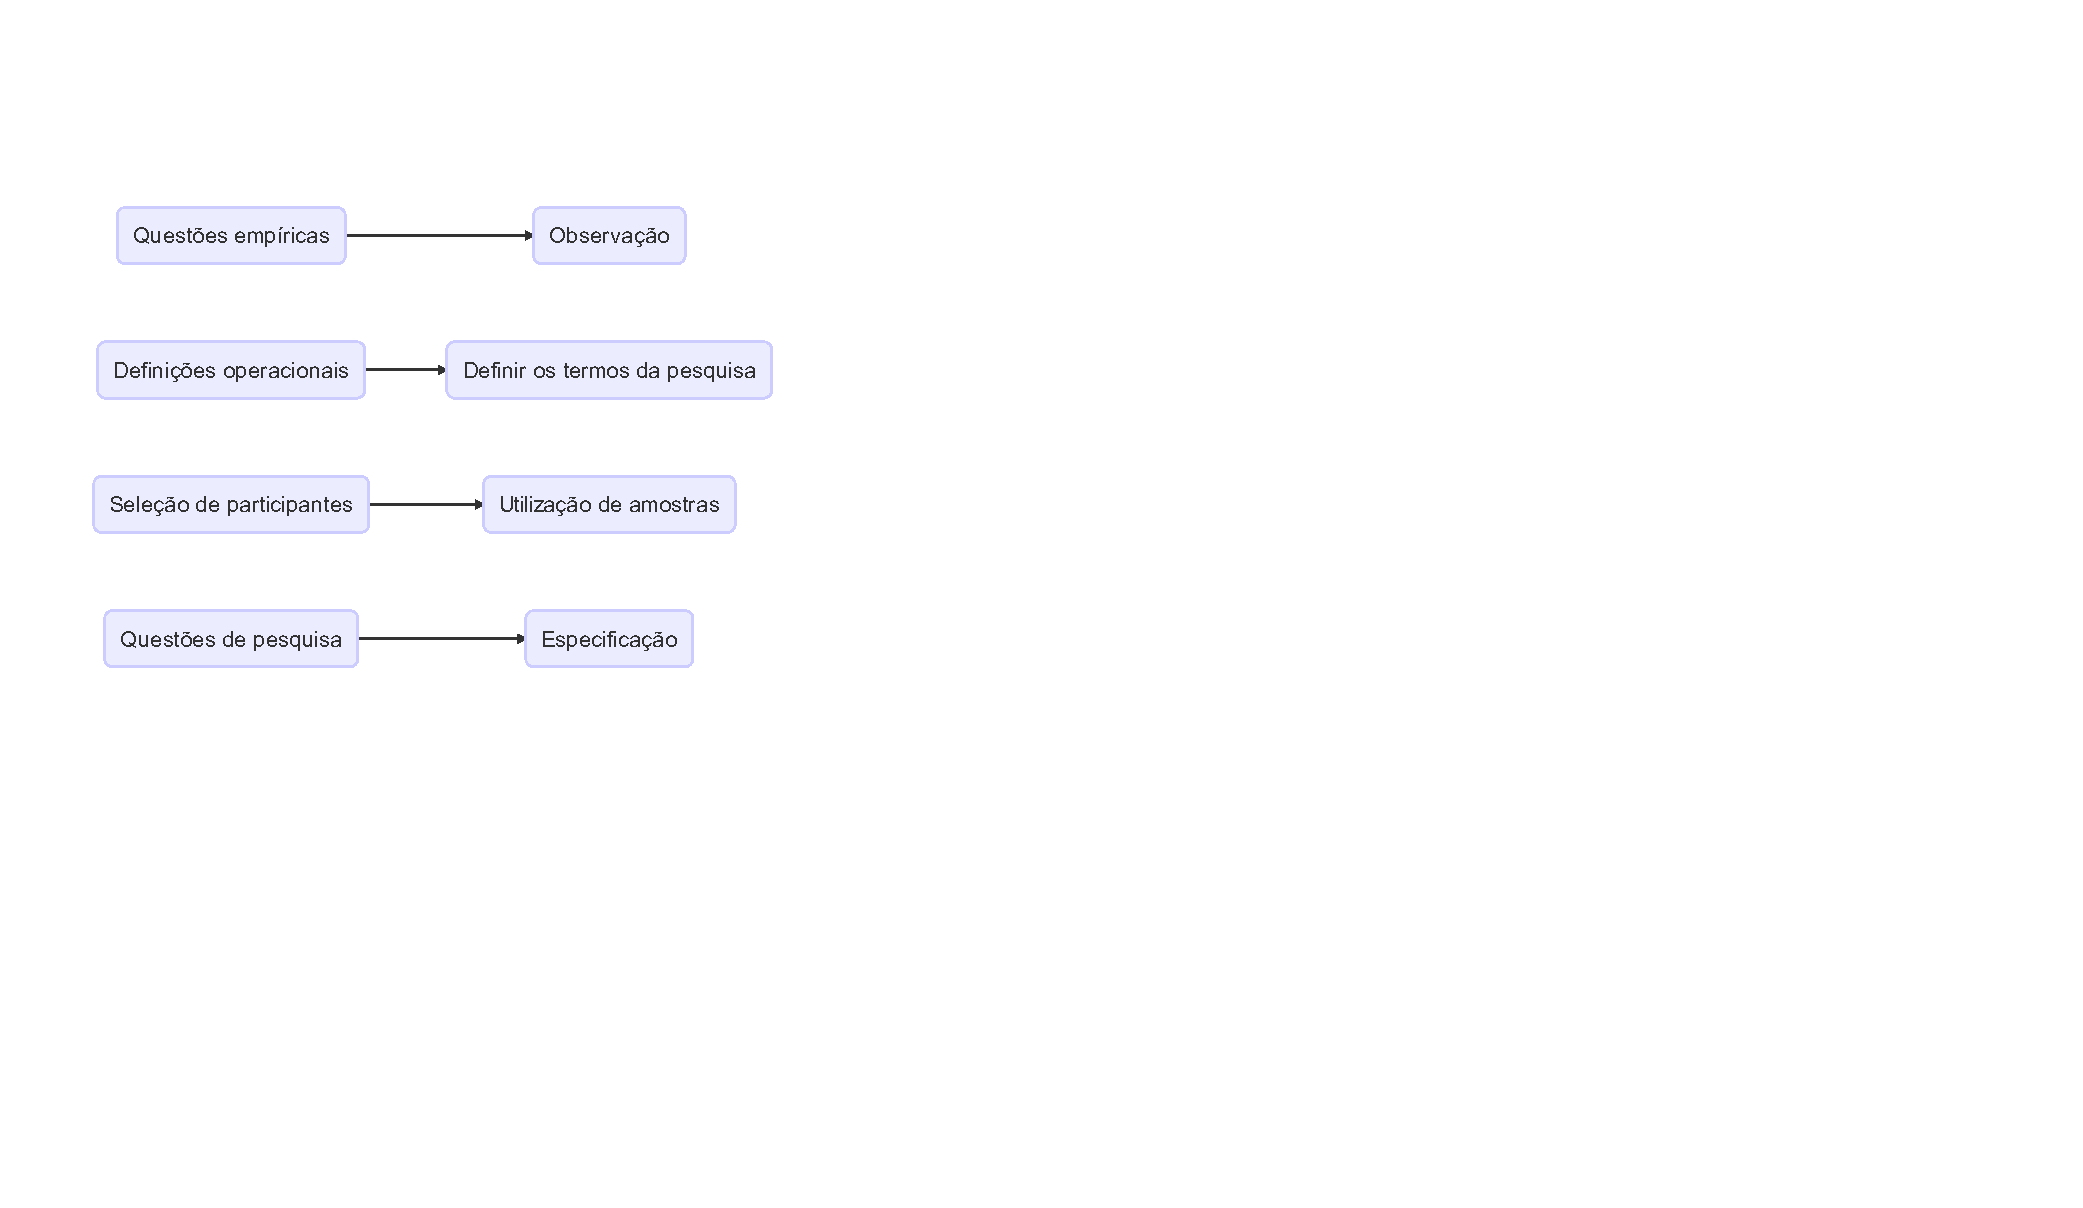
\includegraphics[width=1\linewidth]{Bookdown-Introducao-a-Psicologia_files/figure-latex/Questoes-1}

\hypertarget{apresentauxe7uxe3o-nuxba-02}{%
\section{Apresentação nº 02}\label{apresentauxe7uxe3o-nuxba-02}}

\begin{longtable}[]{@{}ll@{}}
\toprule()
Data & Tópicos Abordados \\
\midrule()
\endhead
dd/mm/aaaa & -Slide ``Metas de Pesquisa em Psicologia'' \\
\bottomrule()
\end{longtable}

\hypertarget{etapas-de-uma-pesquisa}{%
\subsection{Etapas de uma pesquisa}\label{etapas-de-uma-pesquisa}}

Figura - O Método Científico

\begin{itemize}
\tightlist
\item
  As visões do senso comum são frequentemente contraditórias;
\item
  Uma das \textbf{PRIMEIRAS MISSÕES} para o campo da psicologia é \textbf{desenvolver suposições sobre o comportamento} e determinar \textbf{quais dessas suposições são }precisas****;
\item
  Todos os cientistas, incluindo os psicólogos, enfrentam o desafio de ****propor questões apropriadas**** e ****respondê-las**** adequadamente utilizando o ****método científico****;
\item
  O ****método científico****, para os psicólogos:

  \begin{itemize}
  \tightlist
  \item
    Abrange o processo de (1) identificar, (2) formular e (3) responder questões para chegar a uma compreensão sobre o mundo;
  \item
    É uma abordagem usada para ****adquirir**** sistematicamente \textbf{conhecimento} e \textbf{compreensão} sobre:

    \begin{itemize}
    \tightlist
    \item
      o comportamento;
    \item
      outros fenômenos de interesse;
    \end{itemize}
  \item
    Consiste em ****QUATRO PASSOS**** principais:

    \begin{itemize}
    \tightlist
    \item
      \textbf{PASSO 1} - Identificar ****questões de interesse**** (O QUE ?);

      \begin{itemize}
      \tightlist
      \item
        Provinientes de \textbf{comportamento} ou \textbf{fenômeno} que requer explicação;
      \item
        Provinientes de \textbf{descobertas científicas anteriores};
      \item
        Provinientes de curiosidade, criatividade, insight, etc.
      \end{itemize}
    \item
      \textbf{PASSO 2} - Formular uma ****explicação**** (POR QUE ?);

      \begin{itemize}
      \tightlist
      \item
        Especificar uma teoria (Necessária no desenvolvimento de uma hipótese)
      \item
        Desenvolver uma hipótese;\\
      \end{itemize}
    \item
      \textbf{PASSO 3} - Realizar pesquisa destinada a ****apoiar**** ou ****refutar**** a explicação \textbf{utilizando um }método**** (COMO ?);

      \begin{itemize}
      \tightlist
      \item
        Formular uma \textbf{definição operacional} da hipótese;

        \begin{itemize}
        \tightlist
        \item
          A \textbf{definição operacional} é o como (passo a passo) o pesquisador vai colocar em prática o teste da hipótese)
        \end{itemize}
      \item
        Escolher um método de pesquisa;
      \item
        Coletar dados;
      \item
        Analisar dados;
      \end{itemize}
    \item
      \textbf{PASSO 4} - ****Comunicar**** descobertas;
    \end{itemize}
  \end{itemize}
\end{itemize}

Figura - Slide 2 - Página 4

\hypertarget{muxe9todo-cientuxedfico}{%
\subsection{Método Científico}\label{muxe9todo-cientuxedfico}}

\begin{itemize}
\tightlist
\item
  \textbf{Método Não Experimental ( Pesquisa Descritiva )}

  \begin{itemize}
  \tightlist
  \item
    Pesquisa de Arquivo
  \item
    Observações Diretas

    \begin{itemize}
    \tightlist
    \item
      Observações de Laboratório
    \item
      Observações de Campo
    \end{itemize}
  \item
    Pesquisa de Levantamento - Instrumentos de avaliação

    \begin{itemize}
    \tightlist
    \item
      Questionários
    \item
      Entrevistas
    \item
      Testes psicológicos
    \end{itemize}
  \item
    Estudos de Caso
  \item
    Pesquisa Correlacional
  \end{itemize}
\item
  \textbf{Exemplos:}

  \begin{itemize}
  \tightlist
  \item
    \textbf{Objetivo}: Será que desempenho profissional se relaciona com esperança, otimismo e criatividade?
  \item
    \textbf{Hipótese} :O desempenho profissional correlaciona positivamente com esperança, otimismo e criatividade
  \item
    \textbf{Resultados}: A autoavaliação do \textbf{desempenho profissional} se correlacionou positivamente com afetos \textbf{esperança}, \textbf{otimismo} e \textbf{criatividade}.
  \end{itemize}
\item
  \textbf{Método Experimental}

  \begin{itemize}
  \tightlist
  \item
    Pesquisa Experimental ( Estudo experimental )
  \end{itemize}
\end{itemize}

\hypertarget{muxe9todo-cientuxedfico-muxe9todo-nuxe3o-experimental-pesquisa-descritiva}{%
\subsection{Método Científico: Método Não Experimental ( Pesquisa Descritiva )}\label{muxe9todo-cientuxedfico-muxe9todo-nuxe3o-experimental-pesquisa-descritiva}}

Segundo Feldman (2015), é destinada a investigar sistematicamente ****uma pessoa****, ****um grupo**** ou ****padrões de comportamento****.

\hypertarget{i-pesquisa-de-arquivo}{%
\subsection{I ) PESQUISA DE ARQUIVO}\label{i-pesquisa-de-arquivo}}

Slide 2 - Aula 17.08.2022

Não foi detalhado no slide. A professora fez explicações que estão contidas no item abaixo do livro de Introdução a Psicologia de Feldman (2015)\textsuperscript{1}

\begin{quote}
\begin{quote}
\begin{quote}
\begin{quote}
\begin{quote}
\begin{quote}
ACRESCENTAR LINK PARA SECAO DO RESUMO DOS LIVROS
\end{quote}
\end{quote}
\end{quote}
\end{quote}
\end{quote}
\end{quote}

\hypertarget{ii-observauxe7uxe3o-direta-observauxe7uxe3o-naturalista}{%
\subsection{II ) OBSERVAÇÃO DIRETA ( Observação Naturalista )}\label{ii-observauxe7uxe3o-direta-observauxe7uxe3o-naturalista}}

Slide 2 - Aula 17.08.2022

\begin{itemize}
\tightlist
\item
  LABORATÓRIO

  \begin{itemize}
  \tightlist
  \item
    Para observação direta, é a criação em laboratório de um ambiente padrão que estimule o comportamento de interesse e permita a coleta de informações aprimoradas.
  \item
    \textbf{Limitações} da Pesquisa de Laboratório

    \begin{itemize}
    \tightlist
    \item
      Artificialidade;
    \item
      Aplicação das descobertas de laboratório à vida real.
    \end{itemize}
  \end{itemize}
\item
  CAMPO

  \begin{itemize}
  \tightlist
  \item
    Observação naturalista, que implica a observação do comportamento diretamente no seu ambiente natural, sendo mais realista.
  \end{itemize}
\end{itemize}

\begin{quote}
\begin{quote}
\begin{quote}
\begin{quote}
\begin{quote}
\begin{quote}
ACRESCENTAR LINK PARA SECAO DO RESUMO DOS LIVROS
\end{quote}
\end{quote}
\end{quote}
\end{quote}
\end{quote}
\end{quote}

\hypertarget{iii-pesquisa-de-levantamento}{%
\subsection{III ) PESQUISA DE LEVANTAMENTO}\label{iii-pesquisa-de-levantamento}}

Slide 2 - Aula 17.08.2022

\begin{itemize}
\tightlist
\item
  QUESTIONÁRIOS

  \begin{itemize}
  \tightlist
  \item
    Perguntas diretas na coleta de informações sobre o pensamento e o comportamento de um número suficiente de indivíduos.
  \end{itemize}
\item
  ENTREVISTAS

  \begin{itemize}
  \tightlist
  \item
    Similar aos questionários. Os autorrelatos são obtidos diretamente (presencial).
  \item
    Elas se dividem em:

    \begin{itemize}
    \tightlist
    \item
      Estruturadas;
    \item
      Abertas; e
    \item
      Semi-estruturadas.
    \end{itemize}
  \end{itemize}
\item
  TESTES PSICOLÓGICOS

  \begin{itemize}
  \tightlist
  \item
    São projetados para medir conceitos que não podem ser observados diretamente: inteligência, melancolia, traços de personalidade, crenças, sentimentos, etc.
  \end{itemize}
\end{itemize}

\begin{longtable}[]{@{}
  >{\centering\arraybackslash}p{(\columnwidth - 2\tabcolsep) * \real{0.5000}}
  >{\centering\arraybackslash}p{(\columnwidth - 2\tabcolsep) * \real{0.5000}}@{}}
\toprule()
\begin{minipage}[b]{\linewidth}\centering
\end{minipage} & \begin{minipage}[b]{\linewidth}\centering
\end{minipage} \\
\midrule()
\endhead
\textbf{ExemploQuestionário} & \textbf{ExemploEntrevista} \\
\bottomrule()
\end{longtable}

\begin{longtable}[]{@{}
  >{\centering\arraybackslash}p{(\columnwidth - 4\tabcolsep) * \real{0.3333}}
  >{\centering\arraybackslash}p{(\columnwidth - 4\tabcolsep) * \real{0.3333}}
  >{\centering\arraybackslash}p{(\columnwidth - 4\tabcolsep) * \real{0.3333}}@{}}
\toprule()
\begin{minipage}[b]{\linewidth}\centering
\end{minipage} & \begin{minipage}[b]{\linewidth}\centering
\end{minipage} & \begin{minipage}[b]{\linewidth}\centering
\end{minipage} \\
\midrule()
\endhead
\textbf{ExemploTeste NEO PI-R} & \textbf{ExemploTeste de Torrence} & \textbf{ExemploTeste de Autoestima de Rosenberg} \\
Modelo que seja capaz de identificar as dimensões básicas da personalidade, que possa ser compreendido e reconhecido nas diferentes culturas e nacionalidades & Tem por objetivo avaliar algumas dimensões relacionadas ao processo e a personalidade criativa, por meio da produção criativa expressa em forma de desenho & Desenvolvida pelo sociólogo Dr.~Morris Rosenberg, a escala de Rosenberg é uma medida de autoestima amplamente utilizada em pesquisas de ciências sociais. Ele usa uma escala de 0 a 30, em que uma pontuação inferior a 15 pode indicar baixa autoestima problemática. A escala consiste em dez afirmações que você poderia aplicar a você e que deve avaliar o quanto concorda com cada uma. Os itens devem ser respondidos rapidamente, sem pensar demais, sua primeira inclinação é o que você deve anotar. \\
\bottomrule()
\end{longtable}

\hypertarget{iv-estudo-de-caso}{%
\subsection{IV ) ESTUDO DE CASO}\label{iv-estudo-de-caso}}

Slide 2 - Aula 17.08.2022

\begin{itemize}
\tightlist
\item
  Baseiam se na coleta de informações detalhadas sobre um mesmo indivíduo ou grupo, durante um longo período
\end{itemize}

\begin{longtable}[]{@{}
  >{\centering\arraybackslash}p{(\columnwidth - 2\tabcolsep) * \real{0.5000}}
  >{\centering\arraybackslash}p{(\columnwidth - 2\tabcolsep) * \real{0.5000}}@{}}
\toprule()
\begin{minipage}[b]{\linewidth}\centering
\end{minipage} & \begin{minipage}[b]{\linewidth}\centering
\end{minipage} \\
\midrule()
\endhead
\textbf{Estudo de CasoIndividual} & \textbf{Estudo de Casode um Pequeno Grupo} \\
\bottomrule()
\end{longtable}

\begin{quote}
\begin{quote}
\begin{quote}
\begin{quote}
\begin{quote}
\begin{quote}
ACRESCENTAR LINK PARA SECAO DO RESUMO DOS LIVROS
\end{quote}
\end{quote}
\end{quote}
\end{quote}
\end{quote}
\end{quote}

\hypertarget{v-pesquisa-correlacional}{%
\subsection{V ) PESQUISA CORRELACIONAL}\label{v-pesquisa-correlacional}}

Slide 2 - Aula 17.08.2022

\begin{quote}
****ATENÇÃO PARA PROVA:**** \textbf{CORRELAÇÕES NÃO SIGNIFICAM CAUSA !!!}
\end{quote}

\begin{itemize}
\tightlist
\item
  A ****premissa básica**** é de que \textbf{duas variáveis} estão relacionadas.
\item
  Variam em:

  \begin{itemize}
  \tightlist
  \item
    Intensidade (fraco, moderado ou forte)
  \item
    Direção (positivo ou negativo)
  \end{itemize}
\item
  \textbf{VARIÁVEL}: É aquilo que varia. É fenômeno que assume mais de um valor.
\end{itemize}

Exemplo

\begin{itemize}
\tightlist
\item
  \textbf{Objetivo}: Será que \textbf{desempenho profissional} se relaciona com \textbf{esperança}, \textbf{otimismo} e \textbf{criatividade} ?
\item
  \textbf{Hipótese}: O desempenho profissional correlaciona positivamente com esperança, otimismo e criatividade
\item
  \textbf{Resultados}: A autoavaliação do desempenho profissional se correlacionou positivamente com afetos esperança, otimismo e criatividade
\end{itemize}

Figura - Exemplo de pesquisa correlacional

\begin{quote}
\begin{quote}
\begin{quote}
\begin{quote}
\begin{quote}
\begin{quote}
ACRESCENTAR LINK PARA SECAO DO RESUMO DOS LIVROS
\end{quote}
\end{quote}
\end{quote}
\end{quote}
\end{quote}
\end{quote}

\hypertarget{apresentauxe7uxe3o-nuxba-03}{%
\section{Apresentação nº 03}\label{apresentauxe7uxe3o-nuxba-03}}

\begin{longtable}[]{@{}ll@{}}
\toprule()
Data & Tópicos Abordados \\
\midrule()
\endhead
dd/mm/aaaa & -Slide ``Psicanálise x Behaviorismo'' \\
\bottomrule()
\end{longtable}

\begin{itemize}
\tightlist
\item
  Embora os slides estejam disponíveis, ainda não tivemos tempo para elaborar o resumo deles. Vou disponibilizar em breve.
\end{itemize}

\hypertarget{apresentauxe7uxe3o-nuxba-04}{%
\section{Apresentação nº 04}\label{apresentauxe7uxe3o-nuxba-04}}

\begin{longtable}[]{@{}ll@{}}
\toprule()
Data & Tópicos Abordados \\
\midrule()
\endhead
dd/mm/aaaa & -Slide ``Gestalt x Cognição'' \\
\bottomrule()
\end{longtable}

\begin{itemize}
\tightlist
\item
  Embora os slides estejam disponíveis, ainda não tivemos tempo para elaborar o resumo deles. Vou disponibilizar em breve.
\end{itemize}

\hypertarget{apresentauxe7uxe3o-nuxba-05}{%
\section{Apresentação nº 05}\label{apresentauxe7uxe3o-nuxba-05}}

\begin{longtable}[]{@{}ll@{}}
\toprule()
Data & Tópicos Abordados \\
\midrule()
\endhead
dd/mm/aaaa & -Slide ``Abordagem Humanista'' \\
\bottomrule()
\end{longtable}

\begin{itemize}
\tightlist
\item
  Embora os slides estejam disponíveis, ainda não tivemos tempo para elaborar o resumo deles. Vou disponibilizar em breve.
\end{itemize}

Referências

FELDMAN, Robert S. Pesquisa em Psicologia. \emph{In:} Feldman, Robert S. \textbf{Introdução à Psicologia}. 10. ed.~Porto Alegre: AMGH Editora, 2015, p.~26-39

RIBEIRO, Maria Gabriela Costa. \textbf{Slide Introdução à Psicologia}. Introdução à Psicologia. Notas de aula, Faculdade Três Marias, Paraíba 2022.

RIBEIRO, Maria Gabriela Costa. \textbf{Slide Metas de Pesquisa em Psicologia}. Introdução à Psicologia. Notas de aula, Faculdade Três Marias, Paraíba 2022.

RIBEIRO, Maria Gabriela Costa Ribeiro. \textbf{Slide Psicanálise x Behaviorismo}. Introdução à Psicologia, Faculdade Três Marias, Paraíba 2022

RIBEIRO, Maria Gabriela Costa Ribeiro. \textbf{Slide Gestalt x Cognição}. Introdução à Psicologia, Faculdade Três Marias, Paraíba 2022

RIBEIRO, Maria Gabriela Costa Ribeiro. \textbf{Slide Abordagem Humanista}. Introdução à Psicologia, Faculdade Três Marias, Paraíba 2022

SHULTZ, Duane P.; SHULTZ, Sydney Ellen História da psicologia moderna 2014. 10. ed.~São Paulo: Cengage Learning.

\hypertarget{resumo-de-capuxedtulos-de-livros}{%
\chapter{Resumo de Capítulos de Livros}\label{resumo-de-capuxedtulos-de-livros}}

Neste capítulo estarão contidos meus resumos de capítulos de livros.

\hypertarget{livro-psicologias-uma-introduuxe7uxe3o-ao-estudo-da-psicologia-boch-furtado-teixeira-2001}{%
\section{\texorpdfstring{Livro: \textbf{Psicologias Uma Introdução ao Estudo da Psicologia} (BOCH; FURTADO; TEIXEIRA, 2001)}{Livro: Psicologias Uma Introdução ao Estudo da Psicologia (BOCH; FURTADO; TEIXEIRA, 2001)}}\label{livro-psicologias-uma-introduuxe7uxe3o-ao-estudo-da-psicologia-boch-furtado-teixeira-2001}}

\begin{figure}

{\centering 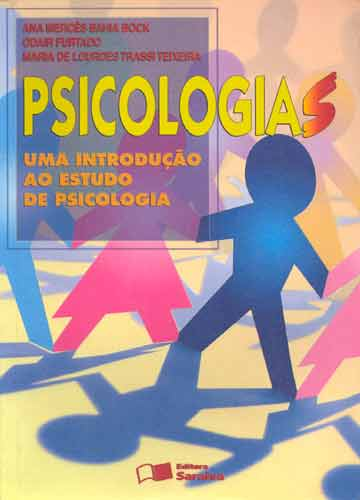
\includegraphics[width=0.5\linewidth]{figuras/LIVRO-PSICOLOGIAS-BOCH} 

}

\caption{Livro Psicologias: Uma Introdução ao Estudo da Psicologia. 13.ed. São Paulo: Saraiva, 2001}\label{fig:unnamed-chunk-2}
\end{figure}

\hypertarget{resumo-do-capuxedtulo-3---o-behaviorismo}{%
\subsection{Resumo do Capítulo 3 - O Behaviorismo}\label{resumo-do-capuxedtulo-3---o-behaviorismo}}

\begin{itemize}
\tightlist
\item
  Em breve, disponibilizaremos.
\end{itemize}

\hypertarget{resumo-do-capuxedtulo-4---a-gestalt}{%
\subsection{Resumo do Capítulo 4 - A Gestalt}\label{resumo-do-capuxedtulo-4---a-gestalt}}

\hypertarget{a-psicologia-da-forma-introduuxe7uxe3o-uxe0-psicologia-da-gestalt}{%
\subsection{A Psicologia da Forma: Introdução à Psicologia da Gestalt}\label{a-psicologia-da-forma-introduuxe7uxe3o-uxe0-psicologia-da-gestalt}}

\begin{itemize}
\tightlist
\item
  Para Bock (2001, p.~59) a Psicologia da Gestalt é uma das tendências
  teóricas mais \textbf{coerentes} e \textbf{coesas} da história da psicologia.
\item
  O termo Gestalt é de origem alemã e tem significado aproximado ao de
  \textbf{forma} ou \textbf{configuração}, porém \textbf{NÃO É
  UTILIZADO} por não corresponder exatamente as seu real significado
  em psicologia.
\item
  No final do século XIII, estudiosos procuravam compreender o
  \textbf{fenômeno psicológico} em seus aspectos
  naturais.

  \begin{itemize}
  \tightlist
  \item
    Principalmente no sentido da \textbf{mensurabilidade} ( A Psicofísica
    em voga ).
  \end{itemize}
\end{itemize}

\hypertarget{predecessores-da-psiologia-da-gestalt}{%
\subsection{Predecessores da Psiologia da Gestalt}\label{predecessores-da-psiologia-da-gestalt}}

\begin{itemize}
\tightlist
\item
  Estudiosos considerados os mais diretos predecessores/antecessores
  da Psisocologia Gestalt:

  \begin{itemize}
  \tightlist
  \item
    Ernst Mash (1838-1916), físico;
  \item
    Christian von Ehrenfels (1859-1932), fisólofo e psicólogo
  \end{itemize}
\item
  Estudos desenvolvidos:

  \begin{itemize}
  \tightlist
  \item
    Estudos psicofísicos sobre as \textbf{sensações} de \textbf{espaço-forma}
    e \textbf{tempo-forma}

    \begin{itemize}
    \tightlist
    \item
      Dado Psicológico: Sensações
    \item
      Dados Físico: espaço-forma e tempo-forma
    \end{itemize}
  \end{itemize}
\end{itemize}

\hypertarget{fundadores-da-psiologia-da-gestalt}{%
\subsection{Fundadores da Psiologia da Gestalt}\label{fundadores-da-psiologia-da-gestalt}}

\begin{itemize}
\tightlist
\item
  Os fundadores da Psicologia da Gestalt construíram a \textbf{base de uma
  teoria psicológica}.
\end{itemize}

\begin{figure}

{\centering 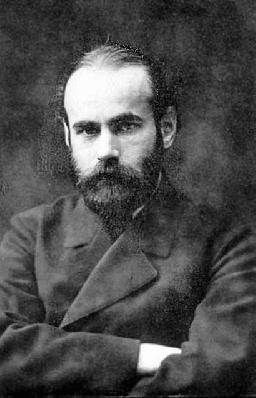
\includegraphics[width=0.3\linewidth]{figuras/MaxWertheimer} 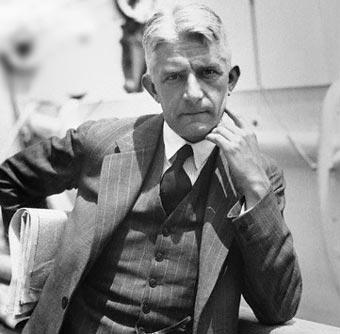
\includegraphics[width=0.3\linewidth]{figuras/WolfgangKohler} 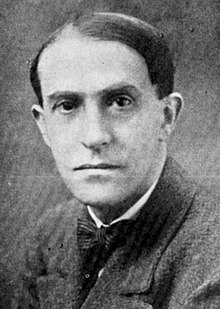
\includegraphics[width=0.3\linewidth]{figuras/KurtKoffka} 

}

\caption{Fundadores da Gestalt: Max Wertheimer | Wolfgang Kohler | Kurt Koffka}\label{fig:unnamed-chunk-3}
\end{figure}

\textbf{Obs}: Clique em :speaker: para ouvir a pronúncia dos nomes dos
cientístas acima.

\begin{itemize}
\tightlist
\item
  Estudos iniciais

  \begin{itemize}
  \tightlist
  \item
    Estudos da percepção e sensação do movimento;
  \item
    Preocupação: Compreender \textbf{quais processos psicológicos}
    estavam envolvidos na \textbf{ilusão de ótica} quando o estímulo é
    percebido como uma \textbf{forma} diferente da que o sujeito tem na
    realidade.

    \begin{itemize}
    \tightlist
    \item
      Exemplo: Cinema; fotogramas estáticos; imagem formada na
      retina que demora um pouco para ser apagada; ilusão de
      óptica do movimento (sensação).
    \end{itemize}
  \end{itemize}
\end{itemize}

\hypertarget{a-percepuxe7uxe3o}{%
\subsection{A percepção}\label{a-percepuxe7uxe3o}}

\begin{itemize}
\tightlist
\item
  É \textbf{ponto de partida} e \textbf{tema central} da Psicologia da Gestalt;
\item
  Teoria Behaviorista

  \begin{itemize}
  \tightlist
  \item
    \textbf{Princípio Implícito}: Há uma relação de \textbf{causa} e
    \textbf{efeito} entre o \textbf{estímulo} e a \textbf{resposta}
  \end{itemize}
\item
  Para Gestaltistas há um questionamento desse \textbf{princípio implícito
  da teoria behaviorista}

  \begin{itemize}
  \tightlist
  \item
    Entre o \textbf{estímulo} e a \textbf{resposta} encontra-se o
    processo de percepção
  \item
    O QUE o indivíduo percebe e
    COMO o indivíduo percebe são
    importantes para entender o COMPORTAMENTO
  \end{itemize}
\end{itemize}

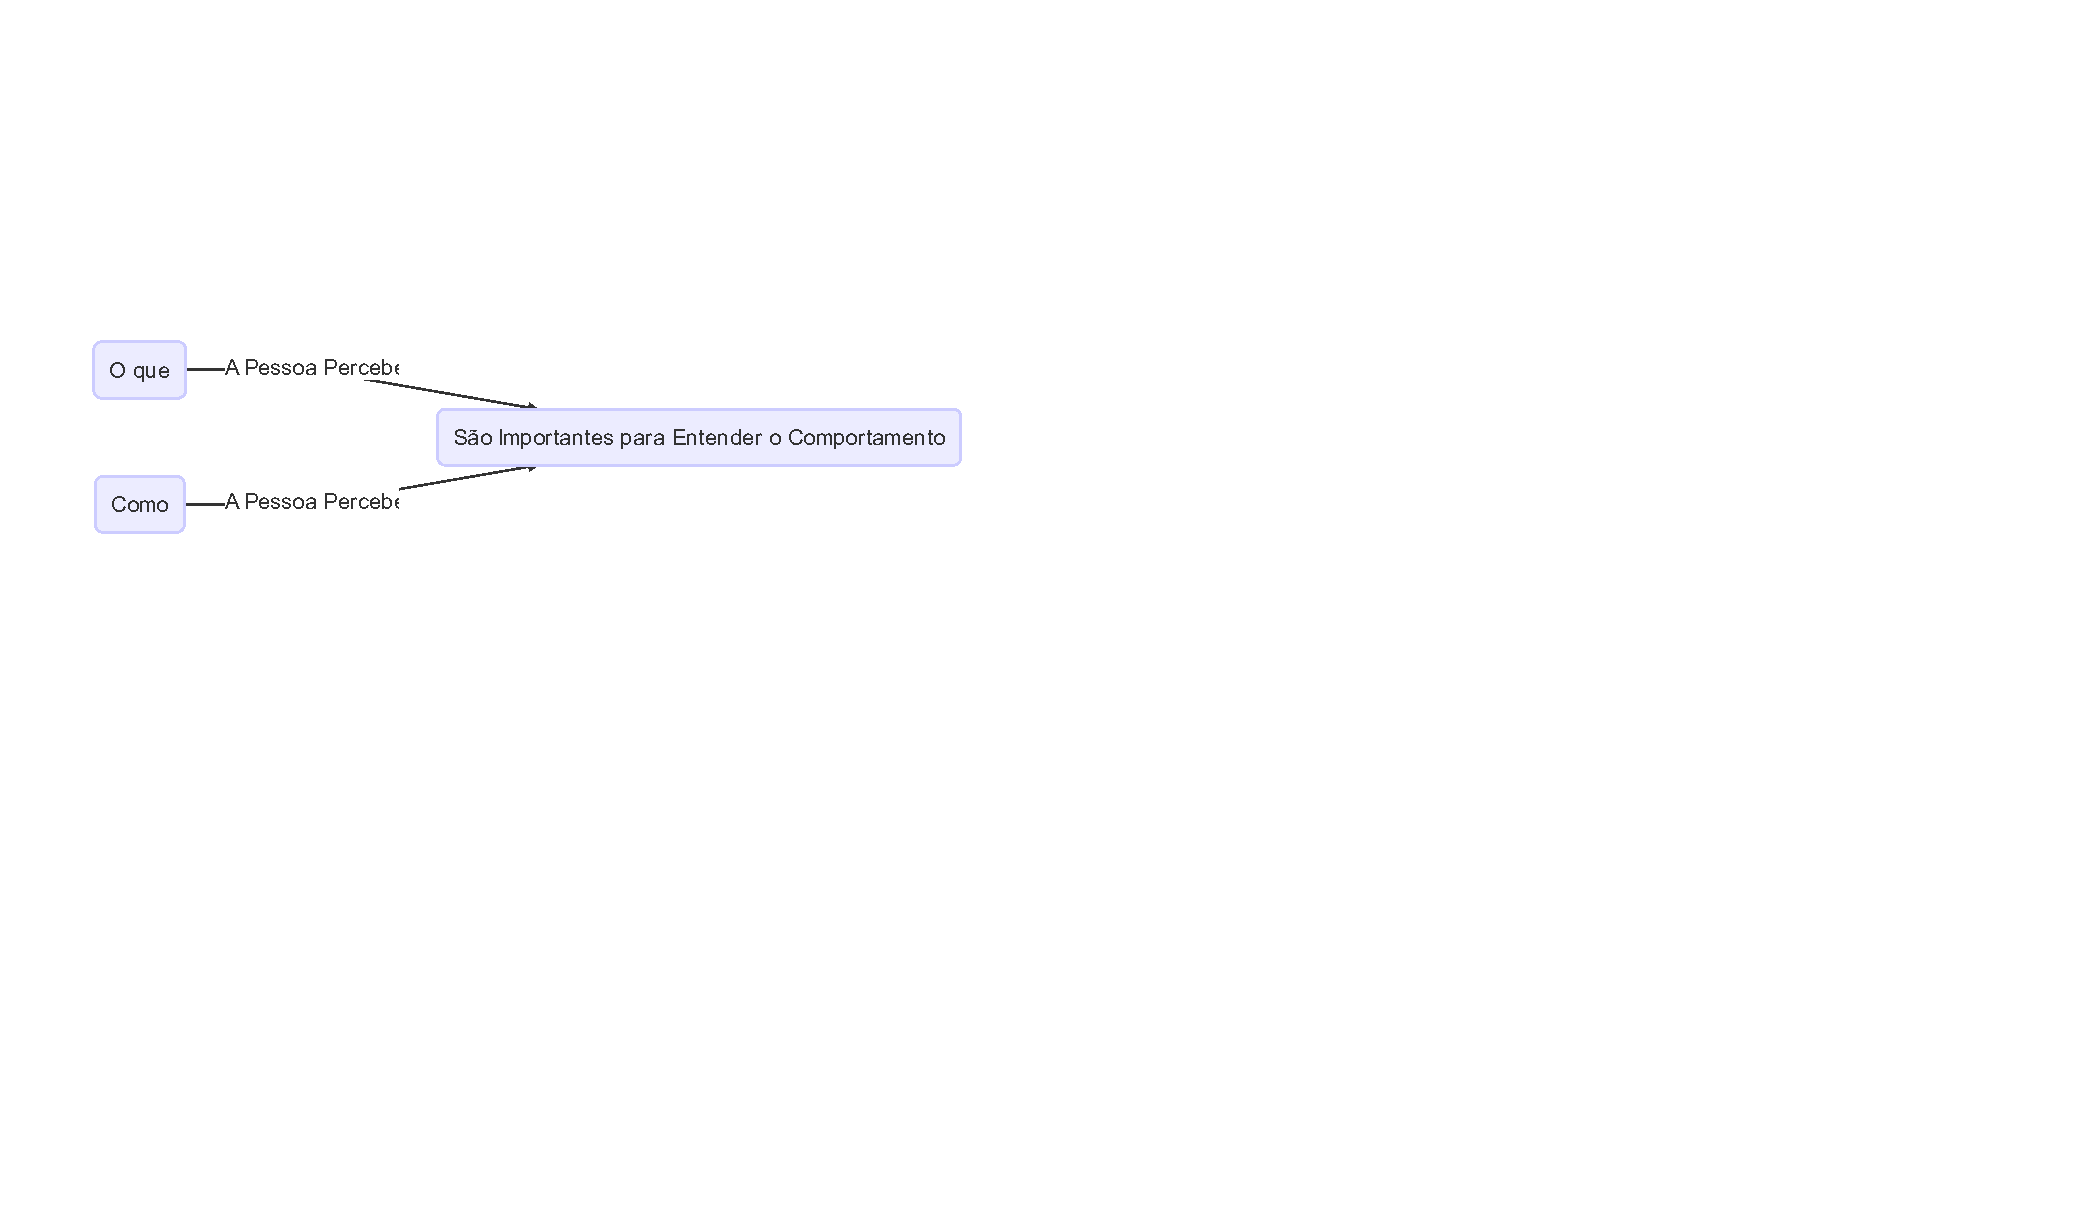
\includegraphics[width=1\linewidth]{Bookdown-Introducao-a-Psicologia_files/figure-latex/unnamed-chunk-4-1}

\hypertarget{posiuxe7uxe3o-de-behavioristas-x-gestaltistas-diante-do-objeto-da-psicologia}{%
\subsection{Posição de Behavioristas x Gestaltistas diante do Objeto da Psicologia}\label{posiuxe7uxe3o-de-behavioristas-x-gestaltistas-diante-do-objeto-da-psicologia}}

\begin{itemize}
\tightlist
\item
  Ambos definem a psicologia como a ciência que estuda o
  COMPORTAMENTO
\item
  Para os Behavioristas:

  \begin{itemize}
  \tightlist
  \item
    É mais profunda a preocupação com a \textbf{objetividade};
  \item
    O \textbf{estudo com comportamento} é feito através da \textbf{relação
    estímulo-resposta};
  \item
    Despreza os conteúdos da consciência pela
    impossibilidade de controlar cientificamente \textbf{essas
    variáveis};
  \item
    Procura isolar o \textbf{estímulo} que corresponderia à \textbf{resposta}
    desprezando conteúdos da consciência pela
    impossibilidade de controlar cientificamente \textbf{essas
    variáveis};
  \end{itemize}
\item
  Para os gestaltistas:

  \begin{itemize}
  \tightlist
  \item
    Há uma \textbf{crítica} a \textbf{abordagem behaviorista} acima;
  \item
    Acreditam que existe um \textbf{contexto mais amplo} que é importante
    no \textbf{estudo do comportamento}

    \begin{itemize}
    \tightlist
    \item
      Esse \textbf{contexto mais amplo} são as
      CONDIÇÕES que \textbf{afetam/alteram} nossa
      capacidade de PERCEBER o \textbf{estímulo};
    \end{itemize}
  \item
    Entendem que estudar o comportamento isolado de um \textbf{contexto
    mais amplo} pode prejudicar o entendimento do comportamento
    pelo psicólogo;
  \item
    O comportamento é estudado em seus aspectos mais globais levando
    em consideração as CONDIÇÕES que
    \textbf{afetam/alteram} nossa capacidade de
    PERCEBER o \textbf{estímulo}
  \end{itemize}
\end{itemize}

\hypertarget{o-que-garante-o-entendimento-do-que-eu-percebo}{%
\subsection{O que Garante o Entendimento do que Eu Percebo ?}\label{o-que-garante-o-entendimento-do-que-eu-percebo}}

\begin{itemize}
\tightlist
\item
  Quando eu vejo

  \begin{itemize}
  \tightlist
  \item
    Uma parte de um objeto
  \end{itemize}
\item
  Ocorre uma tendência à

  \begin{itemize}
  \tightlist
  \item
    restauração do \textbf{equilíbrio da forma}
  \end{itemize}
\item
  Garantindo * O entendimento do que estou percebendo
\end{itemize}

\hypertarget{o-fenuxf4meno-da-percepuxe7uxe3o}{%
\subsection{O Fenômeno da Percepção}\label{o-fenuxf4meno-da-percepuxe7uxe3o}}

\begin{itemize}
\tightlist
\item
  É norteado pela busca de

  \begin{itemize}
  \tightlist
  \item
    \textbf{fechamento} dos pontos que compõem uma figura;
  \item
    \textbf{simetria} dos pontos que compõem uma figura;
  \item
    \textbf{regularidade} dos pontos que compõem uma figura;
  \end{itemize}
\item
  \textbf{Rudolf Arnheim} afirma que o \textbf{sentido normal da visão} apreende
  um \textbf{padrão global};
\end{itemize}

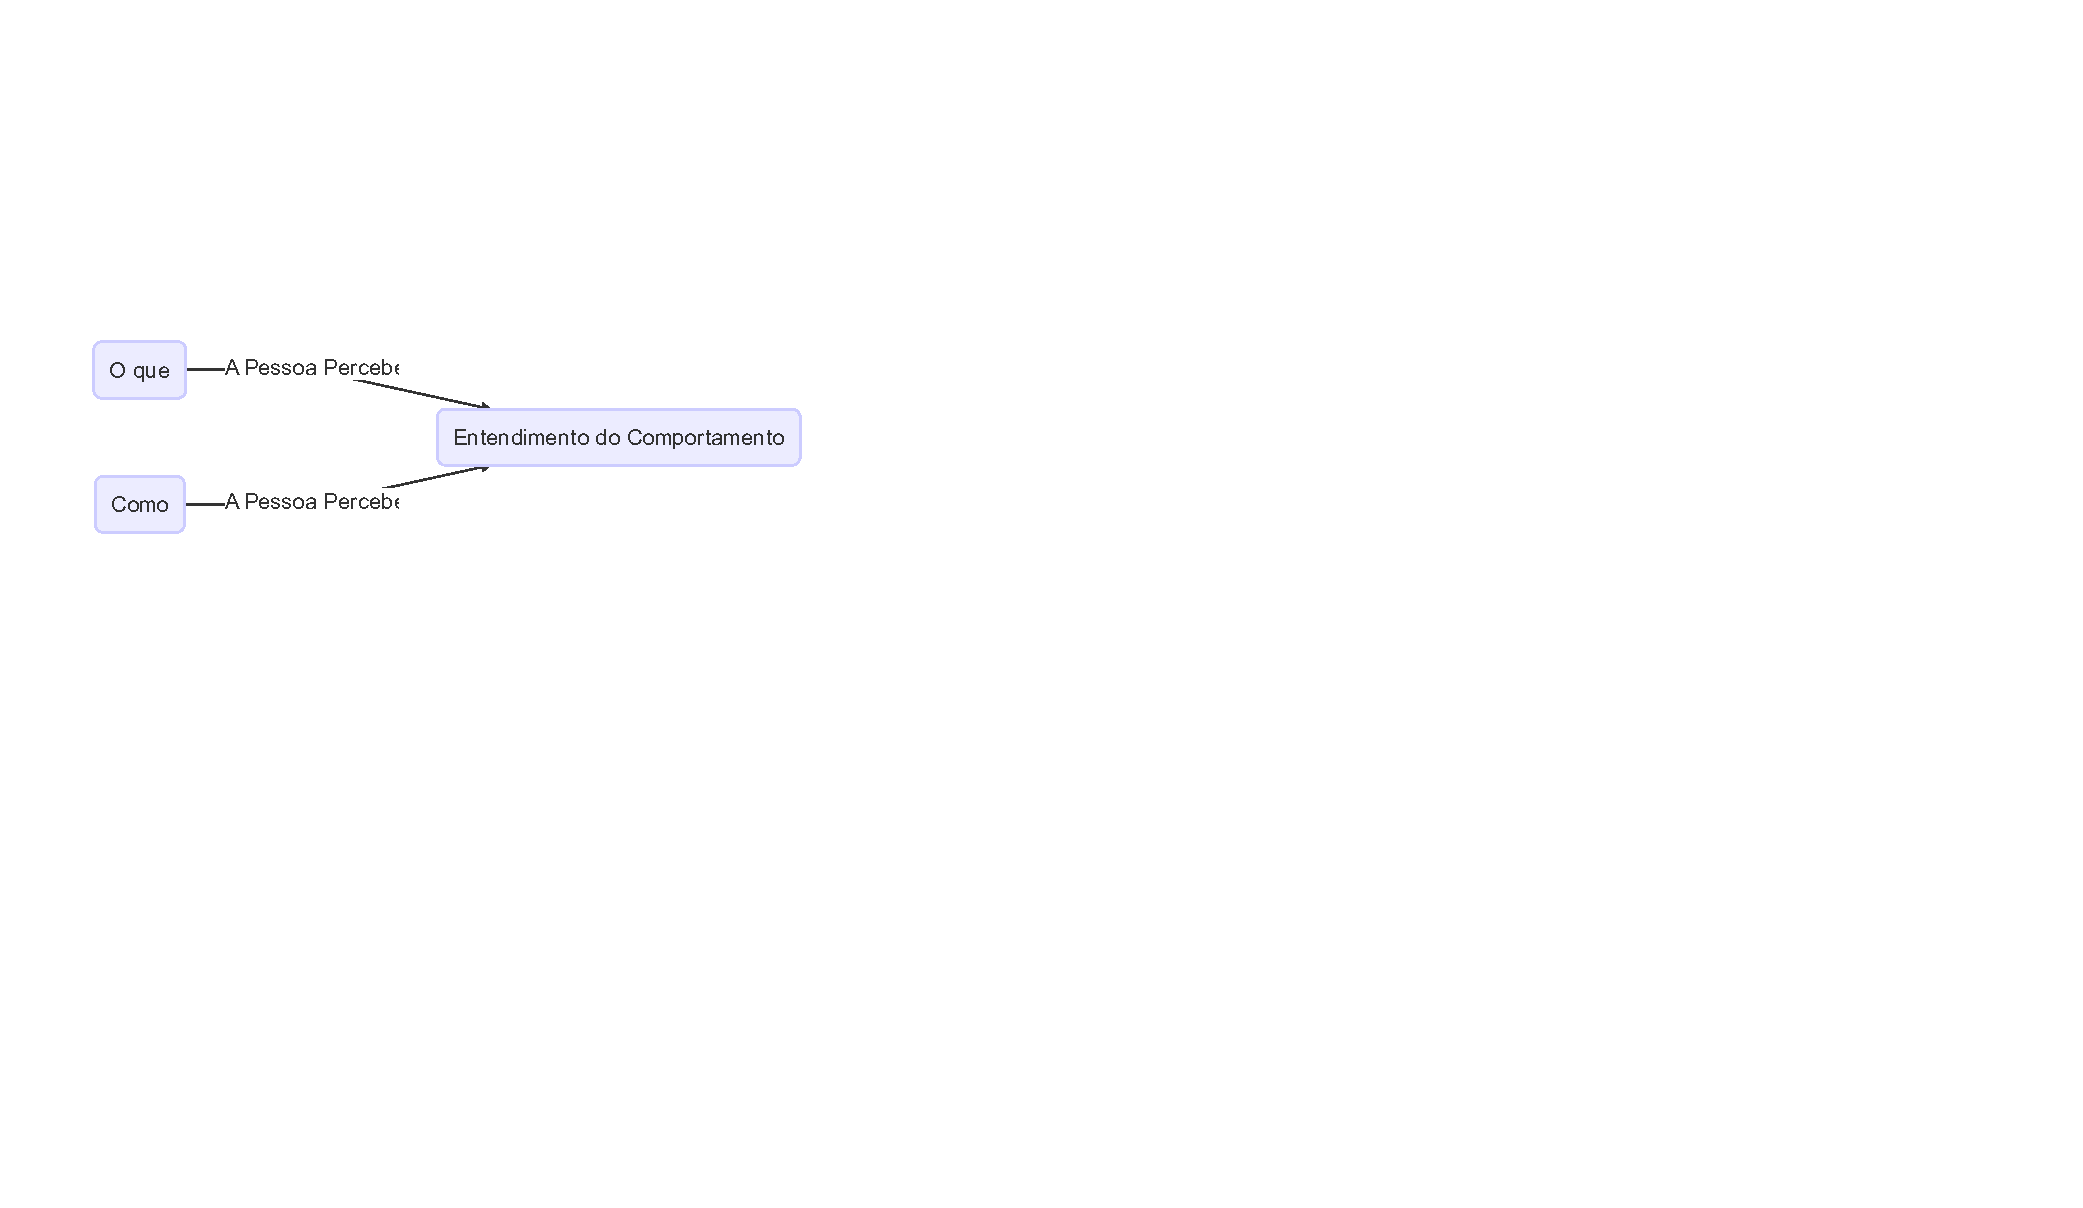
\includegraphics[width=1\linewidth]{Bookdown-Introducao-a-Psicologia_files/figure-latex/unnamed-chunk-5-1}

\begin{figure}

{\centering 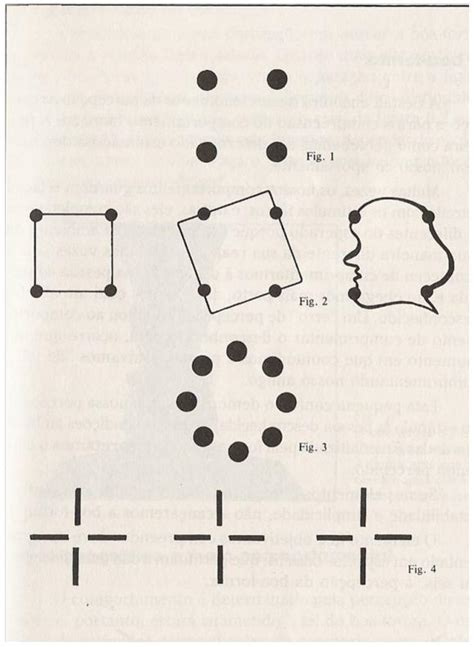
\includegraphics[width=0.6\linewidth]{figuras/gestalt-Lei-basica-da-percepcao-visual} 

}

\caption{Lei básica da percepção visual para os psicólogos da Gestalt}\label{fig:unnamed-chunk-6}
\end{figure}

\begin{itemize}
\tightlist
\item
  Observações a respeito da Figura:

  \begin{itemize}
  \tightlist
  \item
    \textbf{Figura 1}:

    \begin{itemize}
    \tightlist
    \item
      Percebemos como um \textbf{quadrado} e não como uma \textbf{figura
      inclinada} ou um \textbf{perfil} (Figura 2)
    \end{itemize}
  \item
    \textbf{Figura 3}:

    \begin{itemize}
    \tightlist
    \item
      Após acrescentarmos quatro pontos, o padrão percebido na
      Figura 1 irá mudar e perceberemos \textbf{um círculo}
    \end{itemize}
  \item
    \textbf{Figura 4}:

    \begin{itemize}
    \tightlist
    \item
      É possível ver tanto \textbf{círculos brancos} quanto \textbf{quadrados
      brancos} nos centros das cruzes;
    \end{itemize}
  \end{itemize}
\end{itemize}

\begin{quote}
Qualquer padrão de estímulo tende a ser visto de tal modo que a
\textbf{estrutura resultante} é tão \textbf{simples} quanto as \textbf{condições
dadas} permitem
\end{quote}

\hypertarget{a-boa-forma}{%
\subsection{A boa-forma}\label{a-boa-forma}}

\begin{itemize}
\tightlist
\item
  A Psicologia da Gestalt encontra as \textbf{condições} para a
  \textbf{compreensão do comportamento humano} nos \textbf{fenômenos da
  percepção}.
\item
  Em relação aos nossos comportamentos:

  \begin{itemize}
  \tightlist
  \item
    Em alguns casos, \textbf{guardam estreita relação com os estímulos
    físicos};
  \item
    Em outros casos, \textbf{são completamente diferentes do esperado}
    porque ``entendemos o ambiente'' \textbf{de maneira
    diferente da sua realidade}.
  \item
    Exemplo:

    \begin{itemize}
    \tightlist
    \item
      Cumprimentar uma pessoas e depois descobrir que
      cumprimentamos uma pessoa desconhecida (\textbf{Erro de
      Percepção});
    \end{itemize}
  \end{itemize}
\item
  Não há \textbf{boa forma} quando \textbf{nos elementos percebidos} não há:

  \begin{itemize}
  \tightlist
  \item
    Equilíbrio
  \item
    Simetria
  \item
    Estabilidade
  \item
    Simplicidade
  \end{itemize}
\item
  \textbf{O elemento que objetivamos compreender}

  \begin{itemize}
  \tightlist
  \item
    COMO DEVE SER APRESENTADO

    \begin{itemize}
    \tightlist
    \item
      Deve ser apresentado em \textbf{aspectos básicos} que \textbf{permitam
      a sua decodificação} (\textbf{percepção da boa forma})
    \end{itemize}
  \end{itemize}
\end{itemize}

\begin{figure}

{\centering 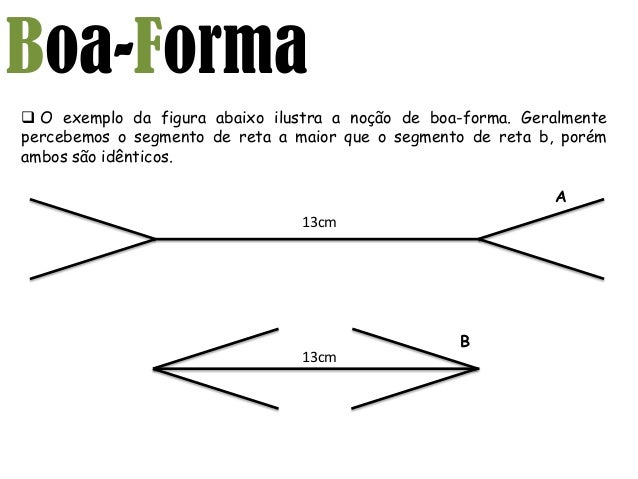
\includegraphics[width=0.7\linewidth]{figuras/gestalt-exemplo-boa-forma} 

}

\caption{Observe a RETA: Elemento que desejamos compreender}\label{fig:unnamed-chunk-7}
\end{figure}

\begin{itemize}
\item
  (\ldots)

  \begin{itemize}
  \tightlist
  \item
    COMO DEVEM SER DISTRIBUÍDOS OS ELEMENTOS QUE COMPÕEM \textbf{O QUE
    DESEJAMOS COMPREENDER} ? * Para garantir a \textbf{boa forma} devem
    ser apresentados com * Equilíbrio * Simetria * Estabilidade
    * Simplicidade
  \end{itemize}
\item
  A \textbf{tendência da nossa percepção} em buscar a \textbf{boa forma}
  permitirá a relação \textbf{figura-fundo}
\item
  Quanto mais clara (simples, estável, simétrica e equilibrada)
  estiver a \textbf{boa-forma}

  \begin{itemize}
  \tightlist
  \item
    Mais clara será a \textbf{separação} entre \textbf{figura} e \textbf{fundo};
  \end{itemize}
\item
  Quanto menos clara estiver a boa forma

  \begin{itemize}
  \tightlist
  \item
    Mais difícil será distinguir o que é figura e o que é fundo
    (Figura Ambígua);
  \end{itemize}

  EM RESUMO
\end{itemize}

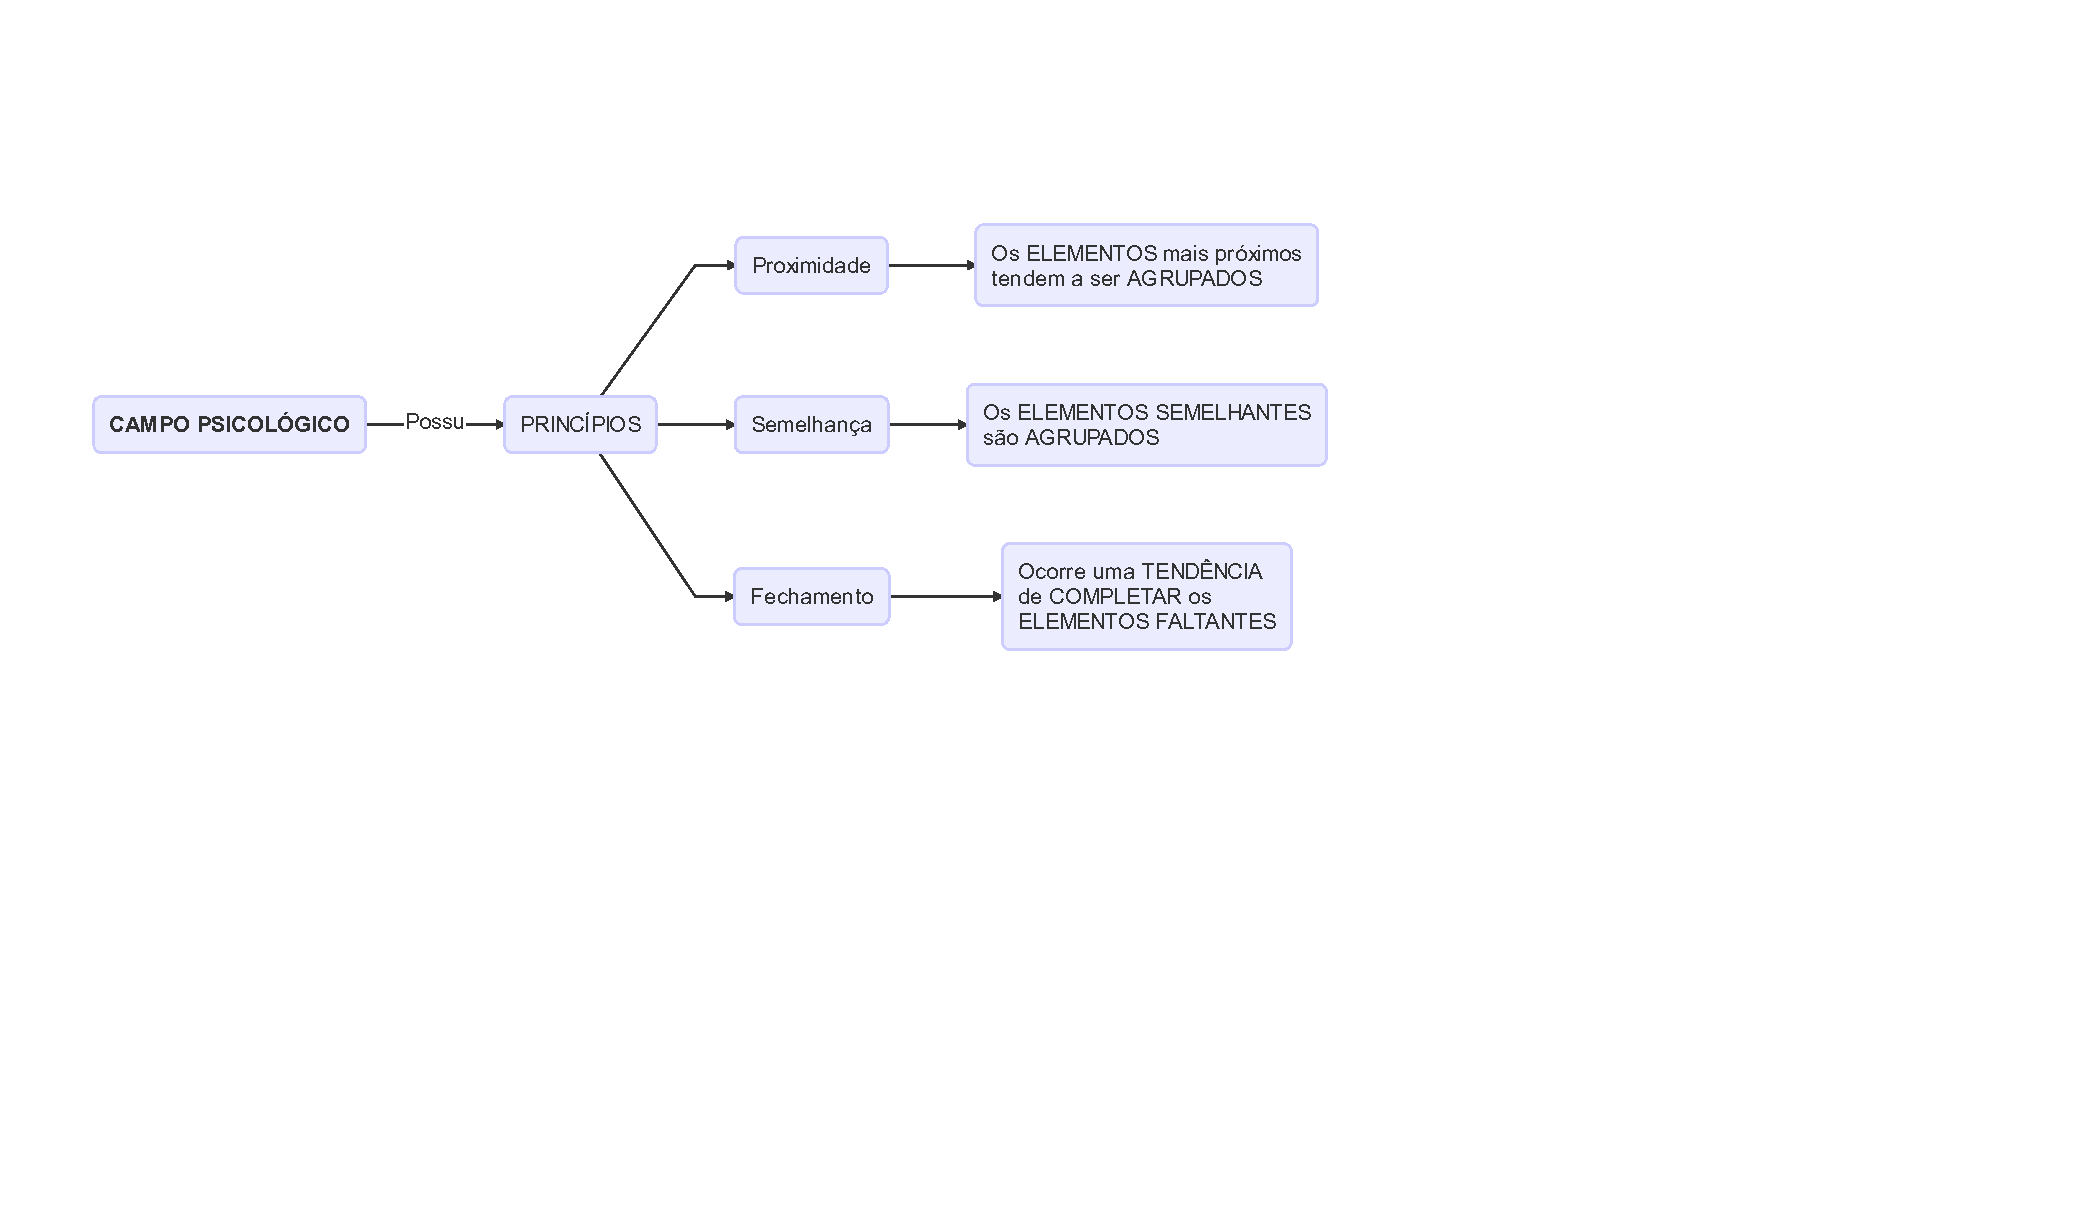
\includegraphics[width=1\linewidth]{Bookdown-Introducao-a-Psicologia_files/figure-latex/unnamed-chunk-8-1}

\hypertarget{meio-geogruxe1fico-e-meio-comportamental}{%
\subsection{Meio Geográfico e Meio Comportamental}\label{meio-geogruxe1fico-e-meio-comportamental}}

\begin{itemize}
\tightlist
\item
  O comportamento \textbf{É DETERMINADO} pela \textbf{PERCEPÇÃO DO
  ESTÍMULO};
\item
  O comportamento está/estará sujeito a \textbf{LEI DA BOA-FORMA};
\item
  O \textbf{CONJUNTO DE ESTÍMULOS} determinantes do comportamento é
  denominado \textbf{MEIO AMBIENTAL} ( ou apenas MEIO )
\item
  Existem DOIS TIPOS DE MEIOS AMBIENTAIS

  \begin{itemize}
  \tightlist
  \item
    \textbf{Meio GEOGRÁFICO}

    \begin{itemize}
    \tightlist
    \item
      É o meio enquanto tal;
    \item
      É o meio físico EM TERMOS OBJETIVOS;
    \end{itemize}
  \item
    \textbf{Meio COMPORTAMENTAL}

    \begin{itemize}
    \tightlist
    \item
      É o meio resultante de INTERAÇÃO (Indivíduo ⇔ Meio Físico)
    \item
      Implica a \textbf{INTERPRETAÇÃO} desse meio através das
      \textbf{FORÇAS} que regem a \textbf{PERCEPÇÃO};

      \begin{itemize}
      \tightlist
      \item
        Forças que regem a percepção:

        \begin{itemize}
        \tightlist
        \item
          Equilíbrio
        \item
          Simetria
        \item
          Estabilidade
        \item
          Simplicidade
        \end{itemize}
      \end{itemize}
    \end{itemize}
  \end{itemize}
\item
  Exemplo

  \begin{itemize}
  \tightlist
  \item
    Cumprimentar uma pessoa desconhecida
  \item
    Se só tivéssemos o \textbf{MEIO GEOGRÁFICO}, essa seria a nossa ÚNICA
    POSSIBILIDADE de percepção;
  \item
    A \textbf{SITUAÇÃO} levou-nos a uma \textbf{INTERPRETAÇÃO DIFERENTE DA
    REALIDADE} e ocorre a confusão com uma pessoa conhecida

    \begin{itemize}
    \tightlist
    \item
      DADOS DA SITUAÇÃO:

      \begin{itemize}
      \tightlist
      \item
        Encontro casual
      \item
        Encontro em movimento
      \item
        Impulso em manifestar uma reação ao encontro
      \end{itemize}
    \end{itemize}
  \item
    No caso desse exemplo

    \begin{itemize}
    \tightlist
    \item
      A semelhança entre as duas pessoas foi \textbf{A CAUSA DO
      ENGANO(=COMPORTAMENTO)}
    \item
      Houve uma tendência em ESTABELECER A UNIDADE DE SEMELHANÇAS
      entre as duas pessoas, MAIS QUE SUAS DIFERÊNÇAS.
    \end{itemize}
  \end{itemize}
\item
  Essa \textbf{TENDÊNCIA A ``JUNTAR'' OS ELEMENTOS} é o que a Gestalt
  denomina de \textbf{FORÇA DE CAMPO PSICOLÓGICO;}
\item
  Nessa \textbf{PARTICULAR INTERPRETAÇÃO DO MEIO} (= O MEIO AMBIENTAL)

  \begin{itemize}
  \tightlist
  \item
    O que PERCEBEMOS é ``UMA REALIDADE'':

    \begin{itemize}
    \tightlist
    \item
      Realidade \textbf{PARTICULAR}
    \item
      Realidade \textbf{OBJETIVA}
    \item
      Realidade \textbf{CRIADA POR NOSSA MENTE}
    \end{itemize}
  \end{itemize}
\end{itemize}

\hypertarget{campo-psicoluxf3gico}{%
\subsection{Campo Psicológico}\label{campo-psicoluxf3gico}}

\begin{itemize}
\tightlist
\item
  Campo psicológico é uma tendência que \textbf{garante} (1) a busca pela
  melhor forma possível \textbf{em situações que não estão muito claras}.
\end{itemize}

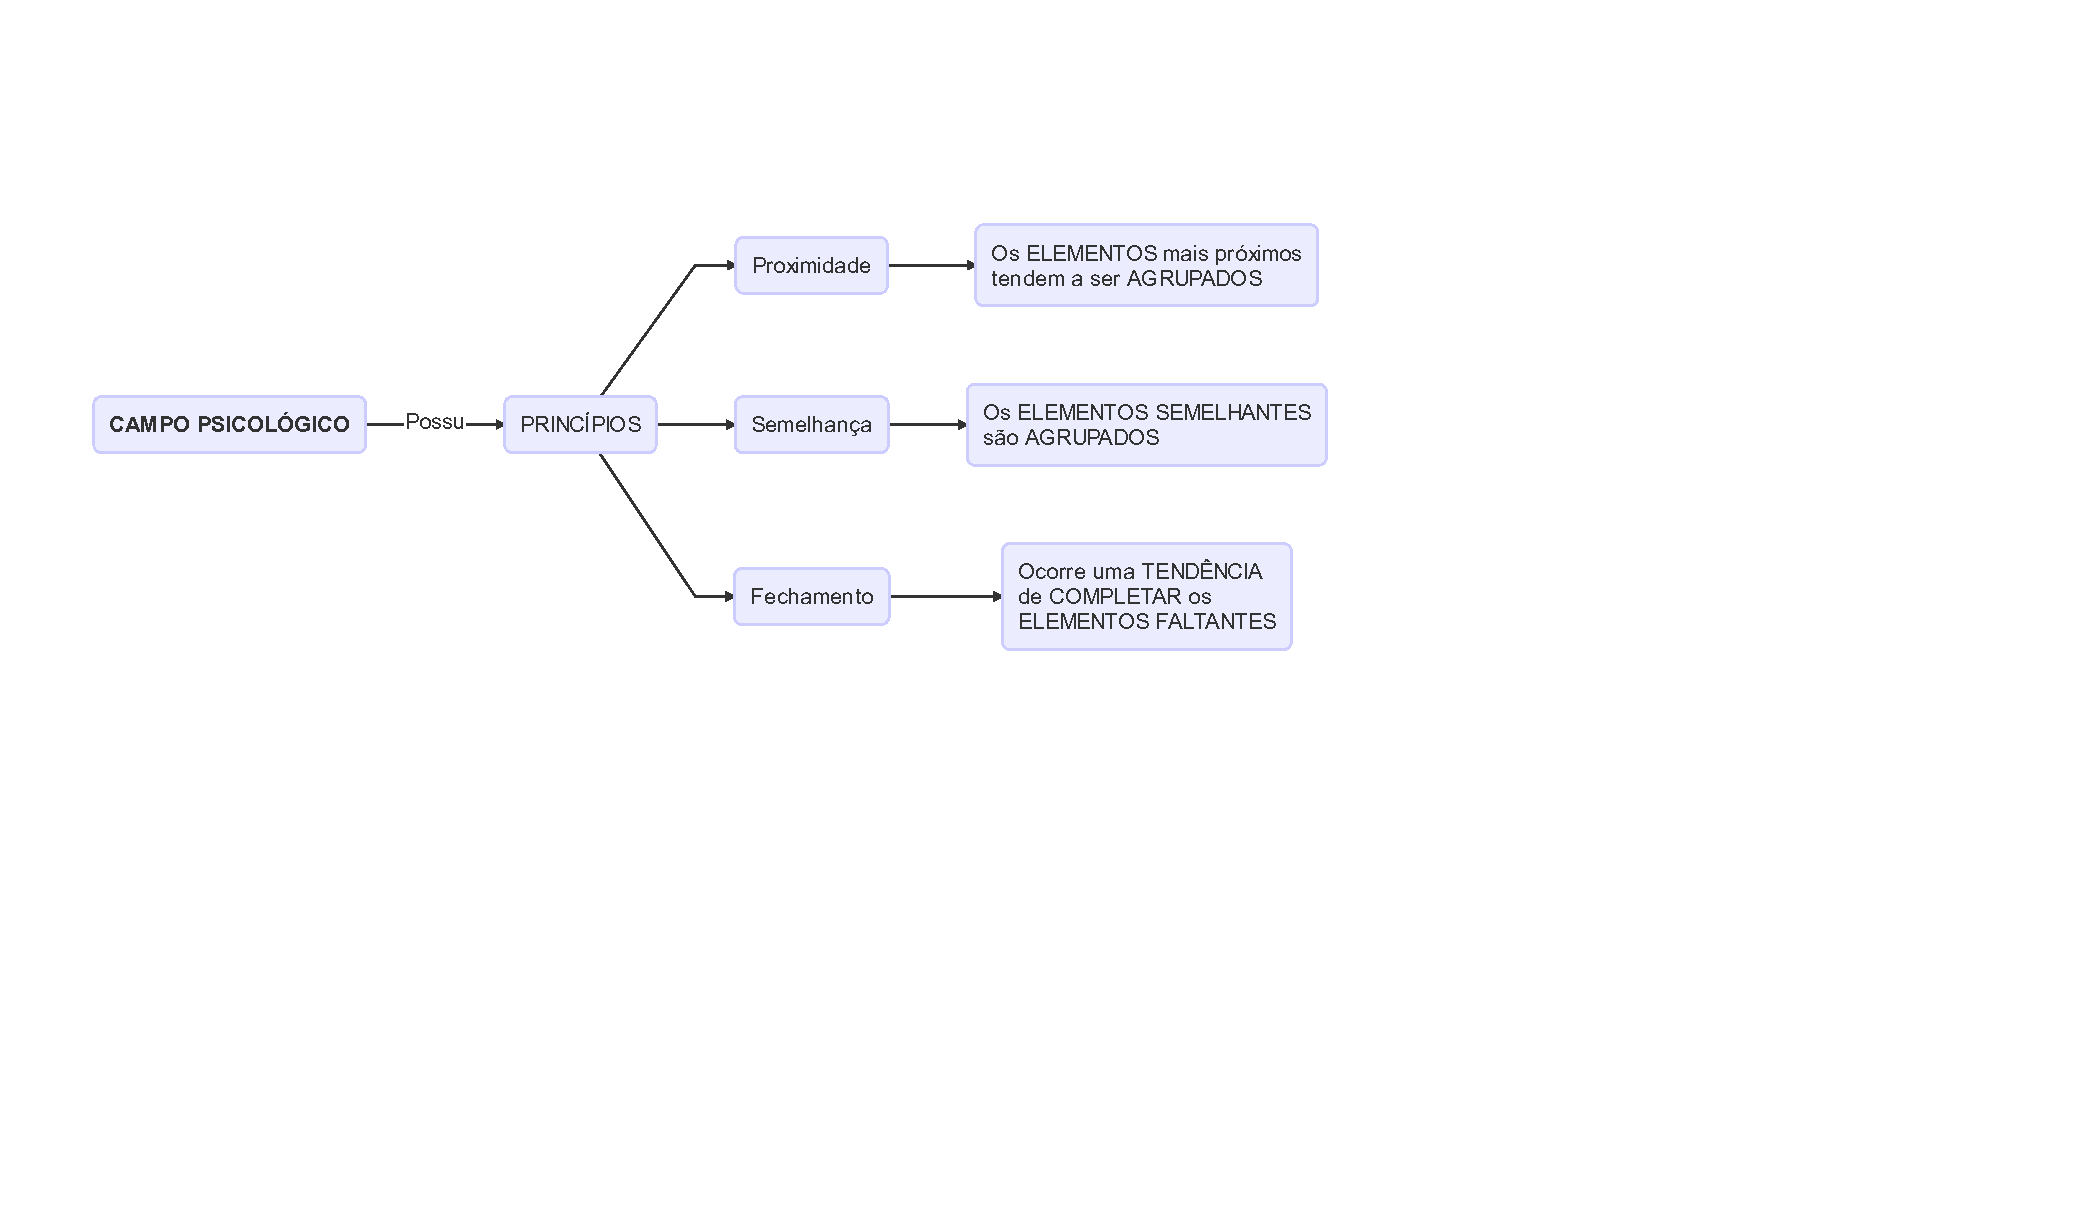
\includegraphics[width=1\linewidth]{Bookdown-Introducao-a-Psicologia_files/figure-latex/unnamed-chunk-9-1}

\hypertarget{princuxedpios-do-campo-psicoluxf3gico}{%
\subsection{Princípios do Campo Psicológico}\label{princuxedpios-do-campo-psicoluxf3gico}}

\begin{itemize}
\tightlist
\item
  O campo psicológico é um processo que ocorre de acordo com
  \textbf{PRINCÍPIOS}:
\end{itemize}

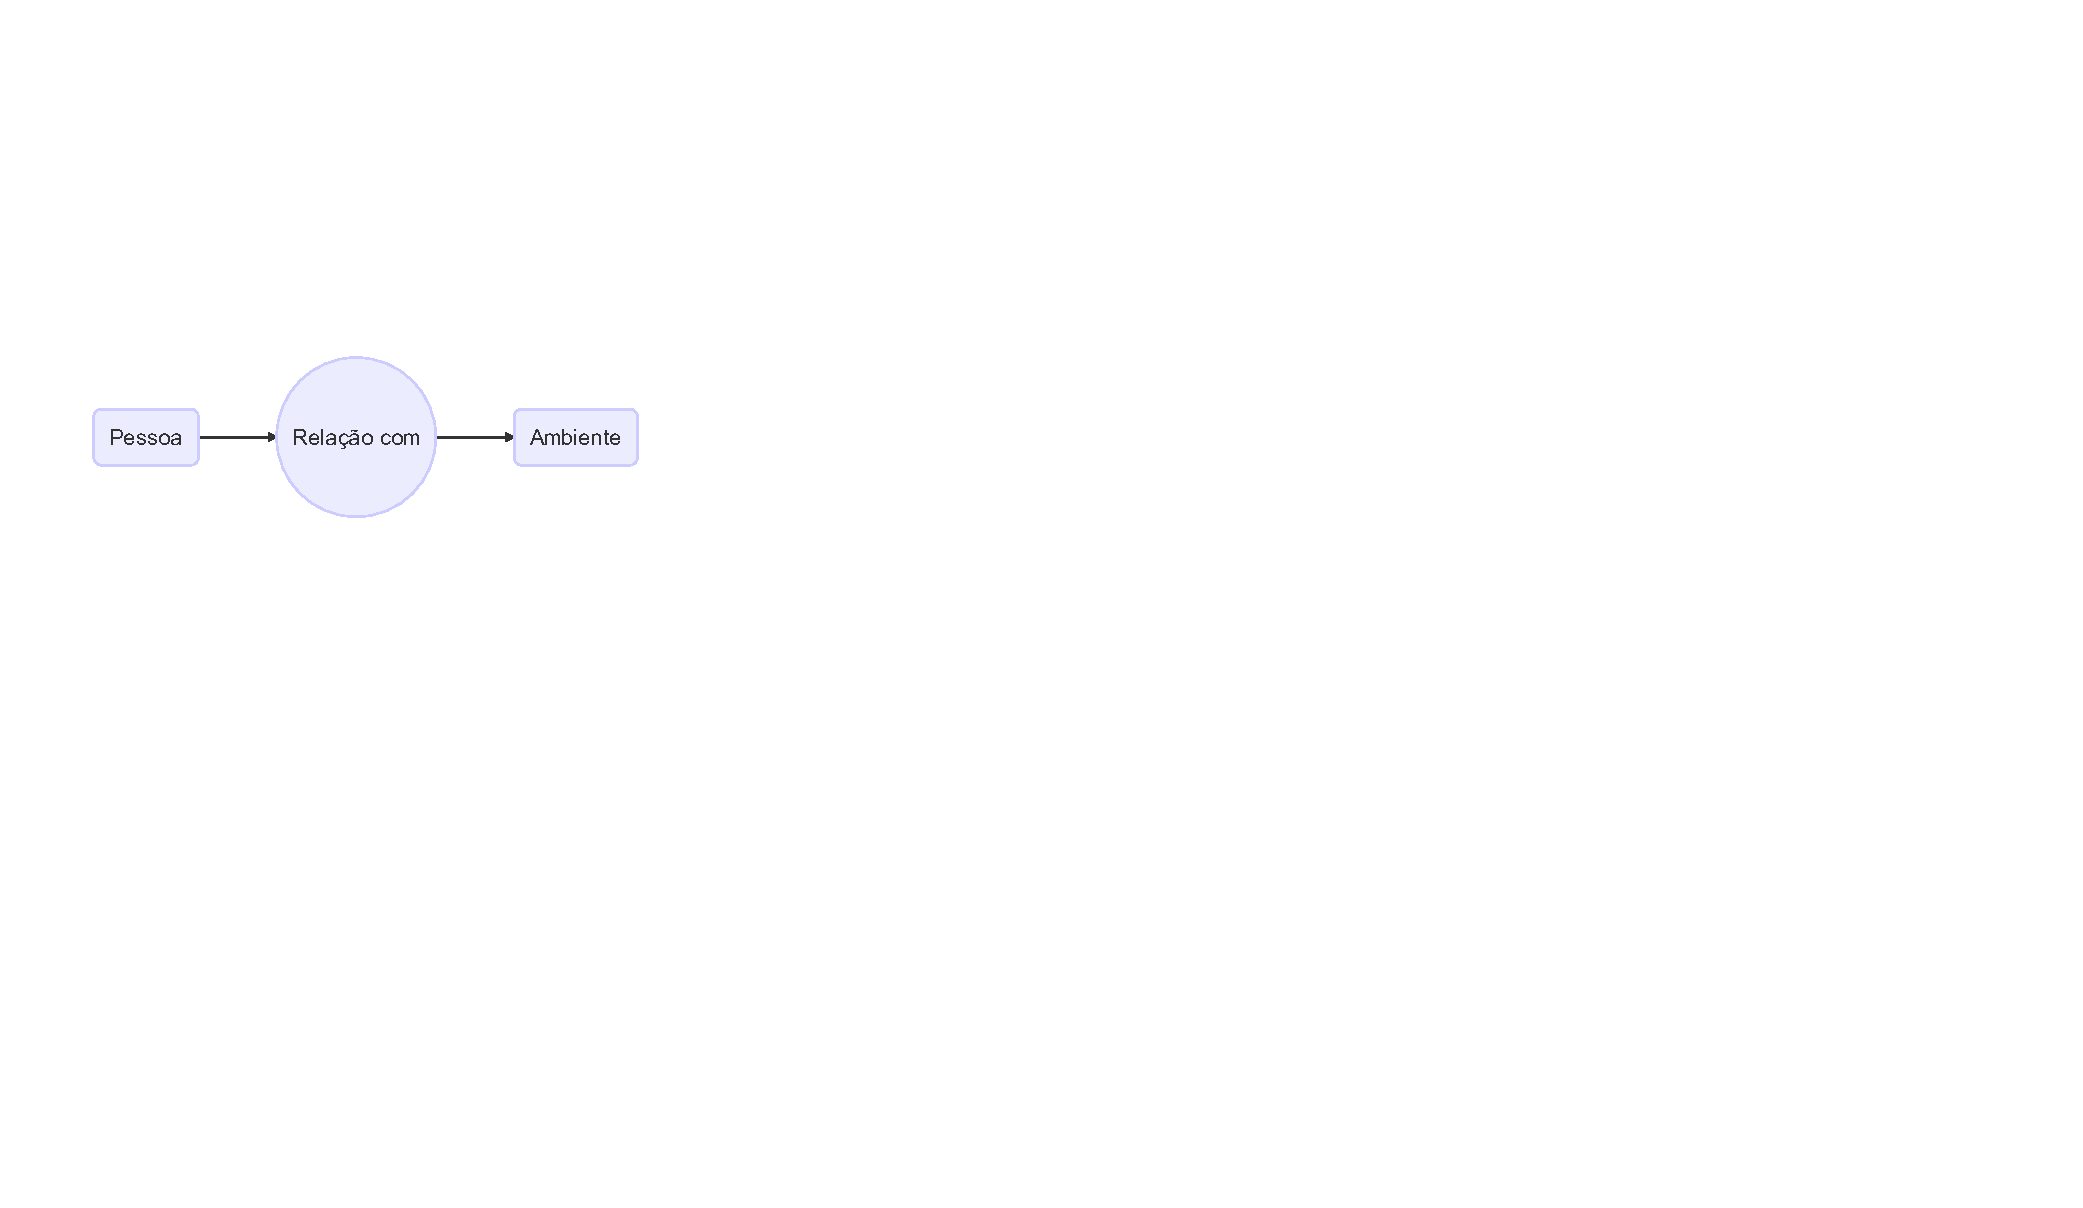
\includegraphics[width=1\linewidth]{Bookdown-Introducao-a-Psicologia_files/figure-latex/unnamed-chunk-10-1}

\hypertarget{insight}{%
\subsection{Insight}\label{insight}}

\begin{itemize}
\tightlist
\item
  Significa \textbf{COMPREENSÃO IMEDIATA};
\item
  Existe uma diferença em como duas correntes psicológicas concebem o
  *\textbf{processo de aprendizagem}:

  \begin{itemize}
  \tightlist
  \item
    \textbf{A Gestalt}

    \begin{itemize}
    \tightlist
    \item
      Acredita que a APRENDIZAGEM é uma RELAÇÃO entre o TODO e a
      PARTE;
    \end{itemize}
  \item
    \textbf{O Associativismo / Behaviorismo}

    \begin{itemize}
    \tightlist
    \item
      Acredita que a APRENDIZAGEM é uma relação de coisas MAIS
      SIMPLES para coisas MAIS COMPLEXAS;
    \end{itemize}
  \end{itemize}
\item
  Na perspectiva da Geltalt, a APRENDIZAGEM é uma relação entre o TODO
  e a PARTE

  \begin{itemize}
  \tightlist
  \item
    Exemplo: É possível uma criança de 03 anos, que não sabe ler,
    distinguir a marca de um refrigerante e nomeá-lo corretamente.

    \begin{itemize}
    \tightlist
    \item
      Ela identificou e SEPAROU a PALAVA em sua TOTALIDADE,
      distinguindo a PALAVRA(figura) e o FUNDO;
    \item
      A criança aprendeu a ler a PALAVRA não juntando as letras,
      mas DANDO SIGNIFICADO ao TODO;
    \end{itemize}
  \end{itemize}
\item
  Nem sempre \textbf{AS SITUAÇÕES VIVIDAS} se apresentam DE FORMA CLARA de
  maneira a permitir uma PERCEPÇÃO IMEDIATA.

  \begin{itemize}
  \tightlist
  \item
    Essas situações DIFICULTAM O PROCESSO DE APRENDIZADO, porque não
    permitem uma clara definição da FIGURA-FUNDO, impedindo a
    relação PARTE/TODO
  \end{itemize}
\end{itemize}

\hypertarget{explicauxe7uxe3o-do-fenuxf4meno-de-insight}{%
\subsection{Explicação do Fenômeno de INSIGHT}\label{explicauxe7uxe3o-do-fenuxf4meno-de-insight}}

\begin{itemize}
\tightlist
\item
  Às vezes, estamos olhando para um \textbf{FIGURA} que \textbf{não tem sentido
  para nós}
\item
  De repente, sem que tenhamos feito nenhum esforço especial, \textbf{A
  RELAÇÃO FIGURA-FUNDOSE ESTABELECE}.
\end{itemize}

\hypertarget{teoria-de-campo-de-kurt-lewin}{%
\subsection{\texorpdfstring{Teoria de Campo de \textbf{Kurt Lewin}}{Teoria de Campo de Kurt Lewin}}\label{teoria-de-campo-de-kurt-lewin}}

\begin{figure}

{\centering 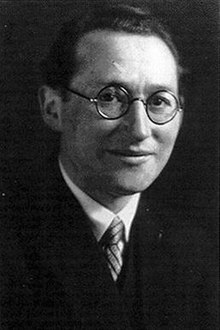
\includegraphics[width=0.4\linewidth]{figuras/KurtLewin} 

}

\caption{Kurt Lewin (1890-1947)}\label{fig:unnamed-chunk-11}
\end{figure}

\hypertarget{kurt-lewin-1890-1947}{%
\subsection{Kurt Lewin (1890-1947)}\label{kurt-lewin-1890-1947}}

\begin{itemize}
\tightlist
\item
  Foi um psicólogo germano-estadunidense pioneiro da Psicologia
  Aplicada, Social e Organizacional nos Estados
  Unidos*.
\item
  Trabalhou 10 anos com os pioneiros da Gestalt: Max Wertheimer,
  Wolfgang Kohler e Kurt Koffka
\item
  Não era um Gestaltista, apesar dessa colaboração, já que ele seguiu
  um caminho teórico diferente desses pioneiros
\item
  Da colaboração com os pioneiros da Gestalt nasceu a \textbf{Teoria de
  Campo}
\item
  Lewin partiu da \textbf{teoria da Gestalt} para construir novos
  conhecimentos para a psicologia.

  \begin{itemize}
  \tightlist
  \item
    Ele abandonou a preocupação \textbf{psicofisiológica}
  \item
    Ele buscou na \textbf{Física} a base metodológica de sua psicologia.
  \end{itemize}
\end{itemize}

\hypertarget{o-conceito-de-espauxe7o-vital-e-de-campo-psicoluxf3gico-de-lewin}{%
\subsection{\texorpdfstring{O Conceito de \textbf{Espaço Vital} e de \textbf{Campo Psicológico} de Lewin}{O Conceito de Espaço Vital e de Campo Psicológico de Lewin}}\label{o-conceito-de-espauxe7o-vital-e-de-campo-psicoluxf3gico-de-lewin}}

CAMPO VITAL

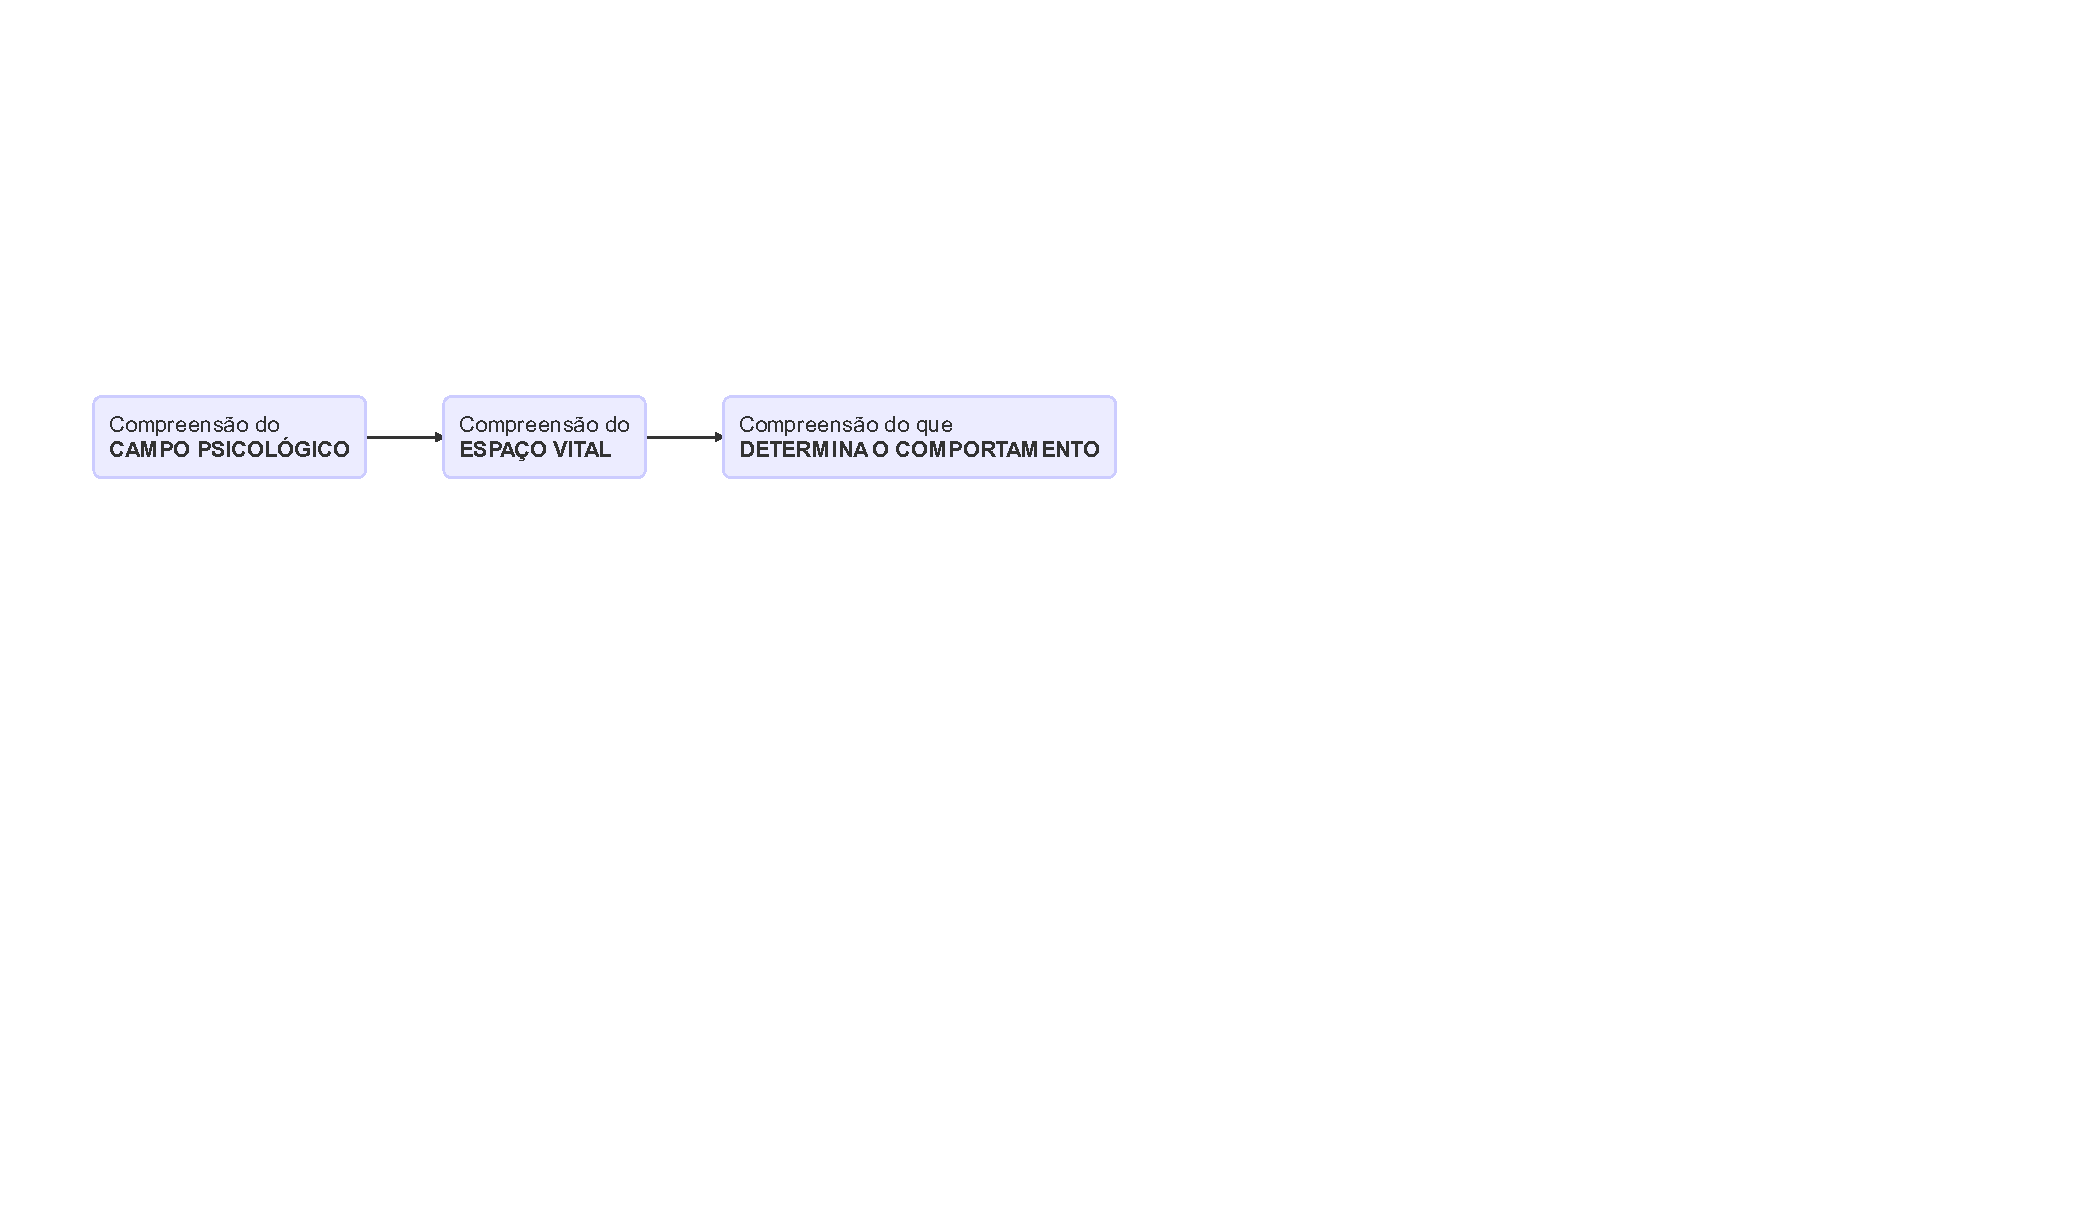
\includegraphics[width=1\linewidth]{Bookdown-Introducao-a-Psicologia_files/figure-latex/unnamed-chunk-12-1}

\begin{itemize}
\tightlist
\item
  A \textbf{DEFINIÇÃO} de \textbf{ESPAÇO VITAL}: ``A \textbf{totalidade dos fatos} que
  DETERMINAM O COMPORTAMENTO do indivíduo, num certo momento''.
\item
  Outro conceito definido por Lewin foi o de \textbf{campo psicológico}: ``É
  o espaço vital considerado dinamicamente'' que deve ser considerado
  (1)tal como ele se apresenta para o indivíduo,
  (2)em um determinado momento.

  \begin{itemize}
  \tightlist
  \item
    Leva-se em conta:

    \begin{itemize}
    \tightlist
    \item
      O indivíduo
    \item
      O meio
    \item
      A \textbf{totalidade dos fatos} coexistentes e
      mutuamente interdependentes
    \end{itemize}
  \end{itemize}
\item
  O CAMPO PSICOLÓGICO \textbf{NÃO É} uma \textbf{realidade física}.
\item
  O CAMPO PSICOLÓGICO \textbf{É} uma \textbf{realidade fenomênica}.
\item
  Para Lewin, \textbf{NÃO SÃO APENAS} fatos físicos que produzem
  efetos sobre o \textbf{comportamento}
\item
  O CAMPO PSICOLÓGICO deve ser representado:

  \begin{itemize}
  \tightlist
  \item
    \textbf{(1) tal como ele existe para o indivíduo},
  \item
    \textbf{(2) num determinado momento}.
  \item
    Ele não existe de forma isolada e estática ( ``\ldots{} e não como ele
    é em si.'').
  \end{itemize}
\item
  São \textbf{ESSENCIAIS} para CONSTRUÇÃO DO CAMPO PSICOLÓGICO:

  \begin{itemize}
  \tightlist
  \item
    Os objetivos CONSCIENTES;
  \item
    Os objetivos INCONSCIENTES;
  \item
    Os sonhos;
  \item
    Os medos;
  \item
    As amizades;
  \item
    O AMBIENTE FÍSICO;
  \end{itemize}
\end{itemize}

\hypertarget{a-realidade-fenomuxeanica-em-kurt-lewin}{%
\subsection{A REALIDADE FENOMÊNICA EM KURT LEWIN}\label{a-realidade-fenomuxeanica-em-kurt-lewin}}

O que é essa realidade fenomênica ?

\begin{enumerate}
\def\labelenumi{\arabic{enumi}.}
\tightlist
\item
  \textbf{A MANEIRA PARTICULAR COMO UM INDIVÍDUO INTERPRETA DETERMINADA
  SITUAÇÃO ➥ MEIO COMPORTAMENTAL da GESTALT}

  \begin{itemize}
  \tightlist
  \item
    \textbf{Obs}: ``A maneira particular como um indivíduo \textbf{INTERPRETA}''
    significa a maneira como cada indivíduo \textbf{PERCEBE} enquanto
    fenômeno psicofisiológico
  \end{itemize}
\item
  As \textbf{CARACTERÍSTICAS DE PERSONALIDADE} do indivíduo;
\item
  Os \textbf{COMPONENTES EMOCIONAIS} ligados à situação \textbf{de vida} e
  \textbf{vivida} própria do indivíduo;
\item
  Os \textbf{COMPONENTES EMOCIONAIS} ligados \textbf{ao grupo} ao qual o
  indivíduo pertence;
\item
  As \textbf{SITUAÇÕES PASSADAS} que estejam ligadas ao acontecimento
\end{enumerate}

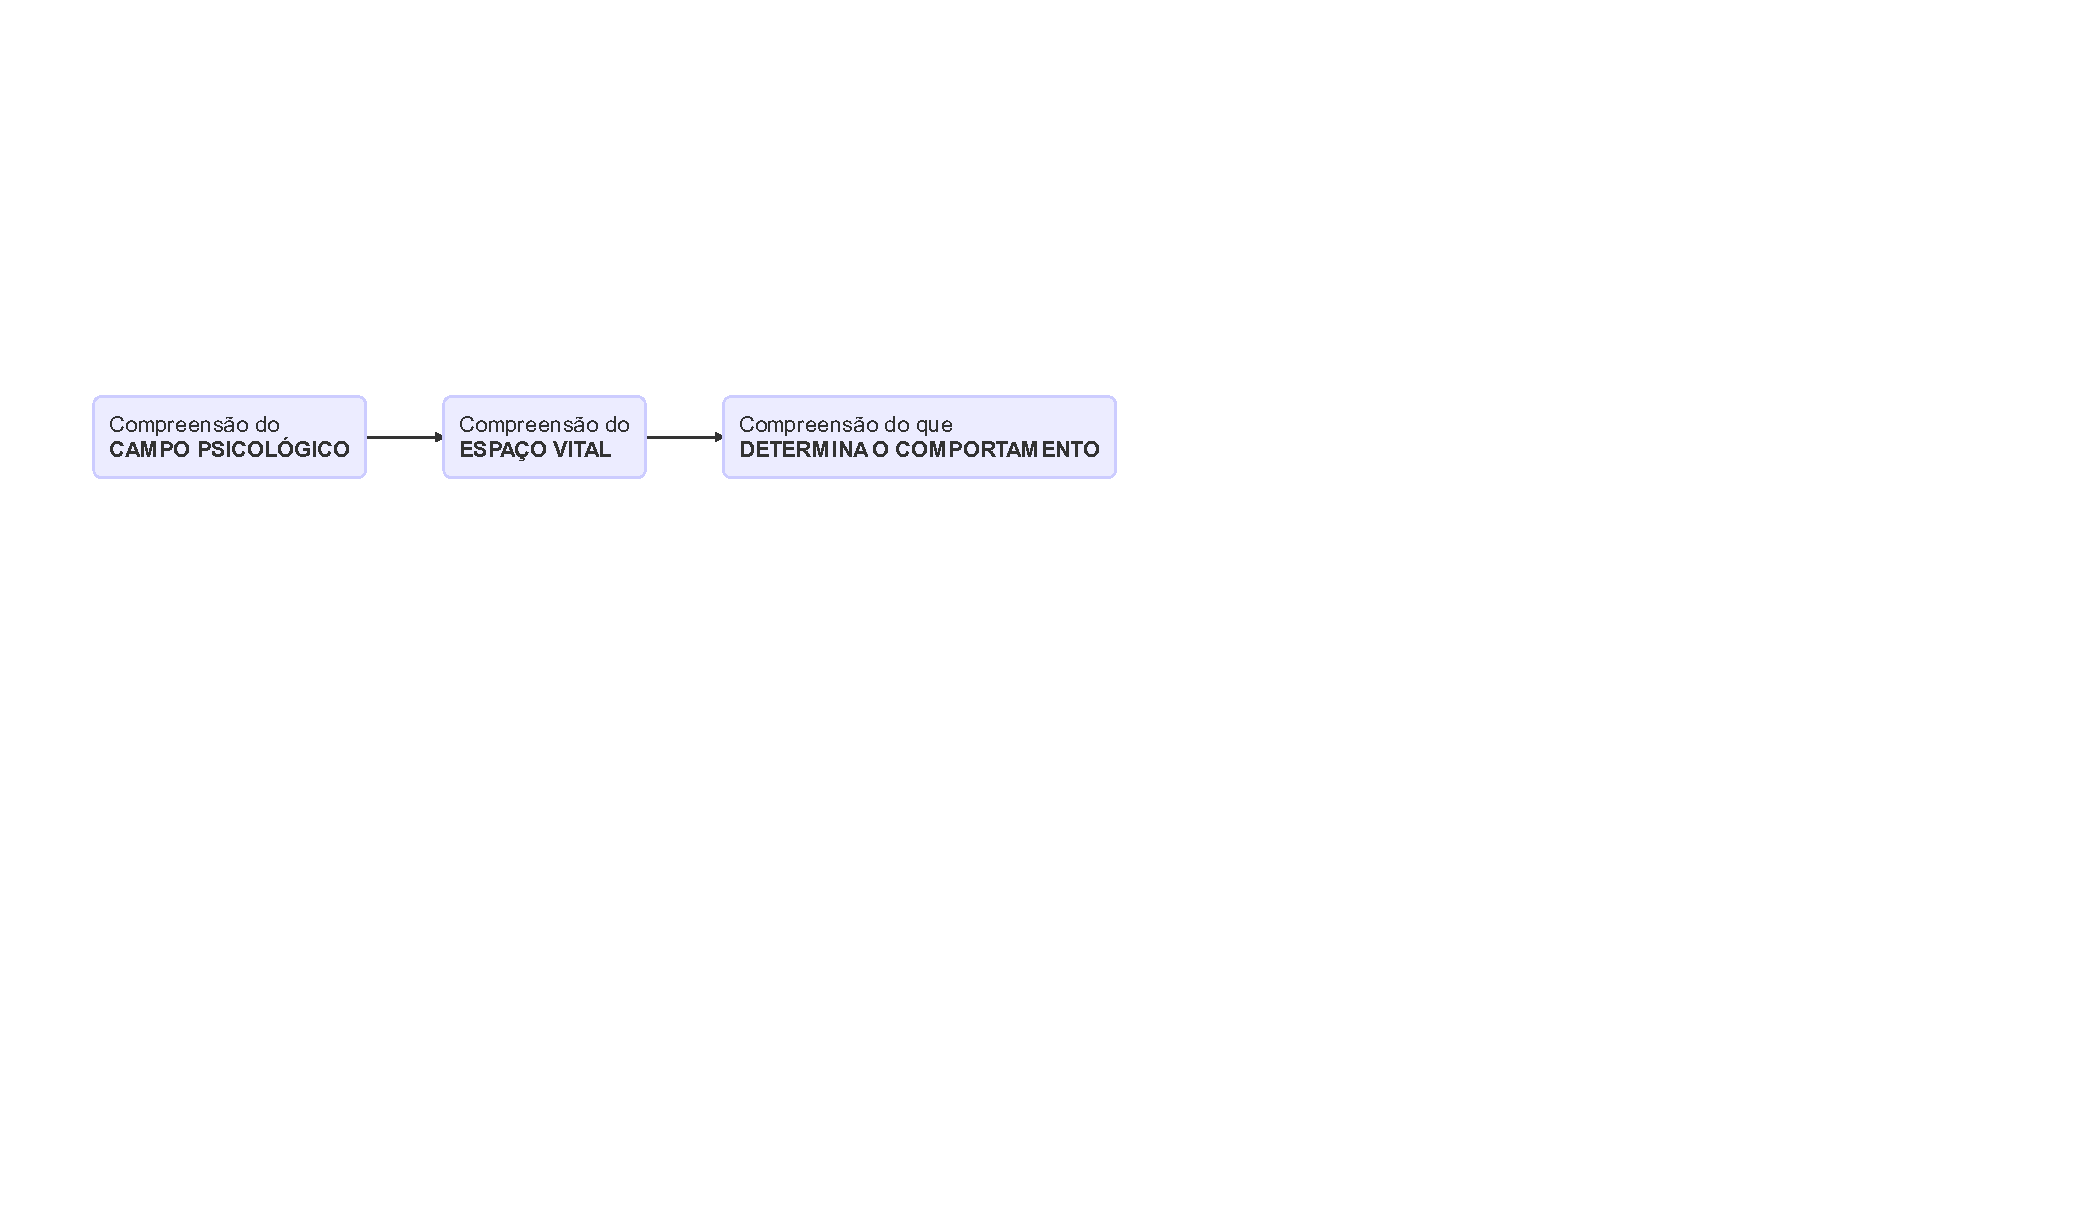
\includegraphics[width=1\linewidth]{Bookdown-Introducao-a-Psicologia_files/figure-latex/unnamed-chunk-13-1}

\hypertarget{exemplo-campo-psicoluxf3gico-e-espauxe7o-vital}{%
\subsection{EXEMPLO: Campo Psicológico e Espaço Vital}\label{exemplo-campo-psicoluxf3gico-e-espauxe7o-vital}}

\begin{enumerate}
\def\labelenumi{\arabic{enumi}.}
\tightlist
\item
  \textbf{RELATO}:
\end{enumerate}

\begin{quote}
Um rapaz, ao chegar a sua casa, surpreende os pais num final de
conversa e escuta o seguinte: ``Ele chegou, é melhor não falarmos disso
agora''. \textbf{Ele entende que} OS PAIS CONVERSAVAM SOBRE UM \textbf{ASSUNTO
SÉRIO}, de que \textbf{ele não deveria tomar conhecimento}. \textbf{RESOLVE não
fazer nenhum comentário sobre o assunto}. Dias depois, chegando
novamente em casa, encontra seus pais na sala com dois homens em
ternos escuros. Imediatamente, associa esses homens ao final da
conversa escutada e entende que eles, de alguma forma, estariam
relacionados às preocupações dos pais.
\end{quote}

\begin{enumerate}
\def\labelenumi{\arabic{enumi}.}
\setcounter{enumi}{1}
\tightlist
\item
  \textbf{COMPORTAMENTO DETERMINADO PELO CAMPO PCISOLÓGICO}:
\end{enumerate}

\begin{itemize}
\tightlist
\item
  ``\textbf{RESOLVE} não fazer comentários sobre o assunto'';
\item
  Ele procurou ``\textbf{fingir que não havia escutado}'';
\end{itemize}

\begin{enumerate}
\def\labelenumi{\arabic{enumi}.}
\setcounter{enumi}{2}
\tightlist
\item
  \textbf{CONSIDERAÇÕES:}
\end{enumerate}

\begin{itemize}
\tightlist
\item
  Nessa estória, o \textbf{CAMPO PSICOLÓGICO} é representado pelas
  \textbf{``linhas de força''} que (1/2)atraem a percepção e
  (2/2)lhe dão significado;
\item
  O rapaz (indivíduo) interpretou a situação pelo seu \textbf{ASPECTO
  FENOMÊNICO} e não pelo que ocorria de fato;
\item
  A INTERPRETAÇÃO ganhou CONSISTÊNCIA com a visita de duas pessoas que
  ele não conhecia (TOTALIDADE DOS FATOS). Isso foi possível porque o
  rapaz havia MEMORIZADO A SITUAÇÃO ANTERIOR e a ela ASSOCIADO A
  SITUAÇÃO SEGUINTE (a nova situações ganhou significado quando ligada
  a situação anterior);
\item
  O ESPAÇO VITAL é a SITUAÇÃO MAIS IMEDIATA ( A que DETERMINOU O
  COMPORTAMENTO );
\item
  O entendimento do \textbf{ESPAÇO VITAL} \textbf{depende diretamente} do
  \textbf{CAMPO PSICOLÓGICO}.
\end{itemize}

A compreensão do que Determina o Comportamento, segundo Kurt
Lewin

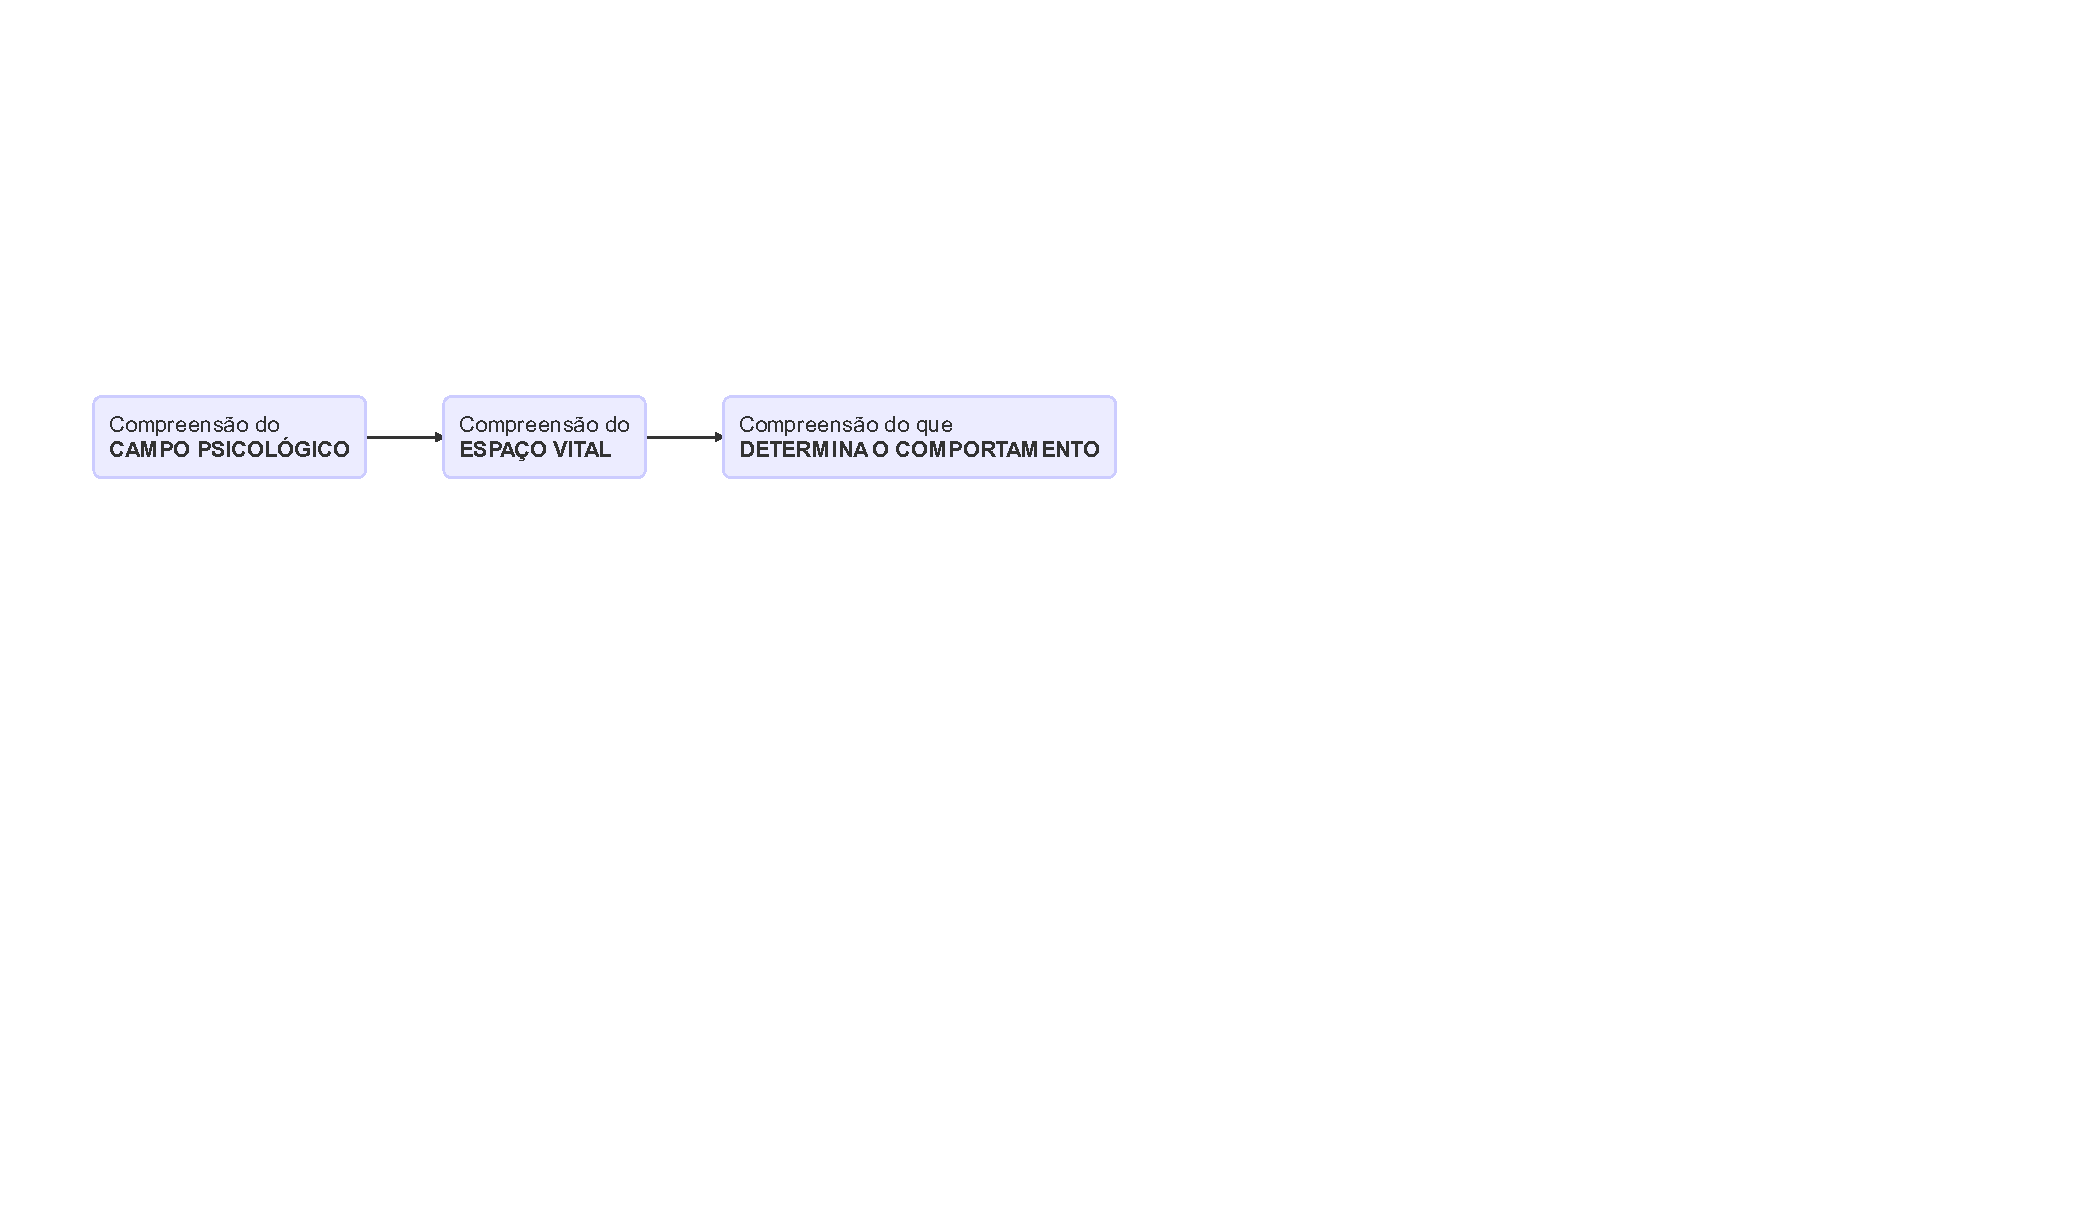
\includegraphics[width=1\linewidth]{Bookdown-Introducao-a-Psicologia_files/figure-latex/unnamed-chunk-14-1}

\hypertarget{a-compreensuxe3o-do-conceito-de-grupo}{%
\subsection{A Compreensão do CONCEITO DE GRUPO}\label{a-compreensuxe3o-do-conceito-de-grupo}}

\begin{itemize}
\tightlist
\item
  Praticamente todos os momentos de nossas vidas OCORREM dentro de
  GRUPOS;
\item
  Para Lewin:

  \begin{itemize}
  \tightlist
  \item
    A \textbf{CARACTERÍSTICA} ESSENCIALMENTE DEFINIDORA DE \textbf{GRUPO} é a
    \textbf{INTERDEPENDÊNCIA} de seus membros.
  \item
    Um grupo não é a \textbf{SOMA DE CARACTERÍSTICAS} de seus membros;
  \item
    Um grupo é \textbf{ALGO NOVO}, resultante dos \textbf{PROCESSOS QUE
    OCORREM} DENTRO DO GRUPO
  \item
    A MUNDANÇA DE UM MEMBRO PODE ALTERAR COMPLETAMENTE A DINÂMICA DO
    GRUPO;
  \end{itemize}
\item
  Os estudos de Lewin:

  \begin{itemize}
  \tightlist
  \item
    Deram ÊNFASE aos \textbf{PEQUENOS GRUPOS};
  \item
    Sobre os GRANDES GRUPOS: Ele considerava que a Psicologia não
    tinha INSTRUMENTAL SUCICIENTE para entender o estudo das GRANDES
    MASSAS;
  \end{itemize}
\end{itemize}

\hypertarget{o-conceito-de-campo-psicoluxf3gico-e-a-psicologia-social}{%
\subsection{O conceito de CAMPO PSICOLÓGICO e a PSICOLOGIA SOCIAL}\label{o-conceito-de-campo-psicoluxf3gico-e-a-psicologia-social}}

\begin{itemize}
\tightlist
\item
  Lewin criou o conceito de CAMPO SOCIAL que é formado pelo GRUPO e
  pelo AMBIENTE;
\item
  Umas das CARACTERÍSTICAS DO GRUPO é o CLIMA SOCIAL;
\item
  Existe uma LIDERANÇA NO GRUPO

  \begin{itemize}
  \tightlist
  \item
    Tipos de LIDERANÇA:

    \begin{itemize}
    \tightlist
    \item
      Autocrática
    \item
      Democrática
    \item
      \emph{Leissez-faire}
    \end{itemize}
  \end{itemize}
\item
  Lewin pesquisou a DINÂMICA GRUPAL atrvés de um TRABALHO EXPERIMENTAL
  minucioso;
\item
  As contribuições de Kurt Lewin:

  \begin{itemize}
  \tightlist
  \item
    Estão presentes até hoje;
  \item
    Embasam:

    \begin{itemize}
    \tightlist
    \item
      OUTRAS TEORIAS que envolvem grupos;
    \item
      TÉCNICAS de trabalho com grupos
    \end{itemize}
  \end{itemize}
\end{itemize}

\hypertarget{resumo-do-capuxedtulo-5---a-psicanuxe1lise}{%
\section{Resumo do Capítulo 5 - A Psicanálise}\label{resumo-do-capuxedtulo-5---a-psicanuxe1lise}}

\begin{itemize}
\tightlist
\item
  Em breve, disponibilizaremos.
\end{itemize}

\hypertarget{resumo-do-capuxedtulo-7---a-psicologia-do-desenvolvimento}{%
\section{Resumo do Capítulo 7 - A Psicologia do Desenvolvimento}\label{resumo-do-capuxedtulo-7---a-psicologia-do-desenvolvimento}}

\begin{itemize}
\tightlist
\item
  Em breve, disponibilizaremos.
\end{itemize}

\hypertarget{livro-teorias-da-personalidade-feist-feist-roberts-2014}{%
\section{\texorpdfstring{Livro: \textbf{Teorias da Personalidade} (FEIST; FEIST; ROBERTS, 2014)}{Livro: Teorias da Personalidade (FEIST; FEIST; ROBERTS, 2014)}}\label{livro-teorias-da-personalidade-feist-feist-roberts-2014}}

\begin{figure}

{\centering 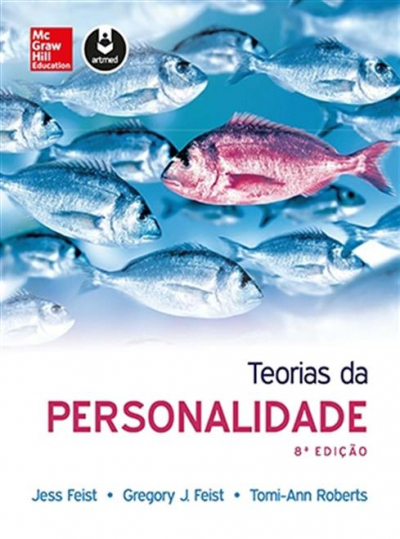
\includegraphics[width=0.8\linewidth]{figuras/Livro-Teorias-da-Personalidade} 

}

\caption{Livro Teorias da Personalidade}\label{fig:unnamed-chunk-15}
\end{figure}

\hypertarget{resumo-do-capuxedtulo-9---maslow-teoria-holuxedstico-dinuxe2mica}{%
\section{Resumo do Capítulo 9 - Maslow: Teoria-Holístico-Dinâmica}\label{resumo-do-capuxedtulo-9---maslow-teoria-holuxedstico-dinuxe2mica}}

\begin{itemize}
\tightlist
\item
  Em breve, disponibilizaremos.
\end{itemize}

\hypertarget{resumo-do-capuxedtulo-10---rogers-teoria-centrada-na-pessoa}{%
\section{Resumo do Capítulo 10 - Rogers: Teoria Centrada na Pessoa}\label{resumo-do-capuxedtulo-10---rogers-teoria-centrada-na-pessoa}}

\begin{itemize}
\tightlist
\item
  Em breve, disponibilizaremos.
\end{itemize}

\hypertarget{livro-introduuxe7uxe3o-uxe0-psicologia-feldman-2015}{%
\section{\texorpdfstring{Livro: \textbf{Introdução à Psicologia} (FELDMAN, 2015)\protect\hyperlink{feldman}{*}}{Livro: Introdução à Psicologia (FELDMAN, 2015)*}}\label{livro-introduuxe7uxe3o-uxe0-psicologia-feldman-2015}}

Figura Livro - FELDMAN, Robert S. \textbf{Introdução à Psicologia}.
10.ed. Porto Alegre: AMGH Editora, 2015

\hypertarget{capuxedtulo-1---muxf3dulo-3---livro-introduuxe7uxe3o-uxe0-psicologia}{%
\subsection{Capítulo 1 - Módulo 3 - Livro Introdução à Psicologia}\label{capuxedtulo-1---muxf3dulo-3---livro-introduuxe7uxe3o-uxe0-psicologia}}

Capítulo 1 - Módulo 3 - Livro Introdução à
Psicologia1

\begin{itemize}
\tightlist
\item
  Na pesquisa de arquivo, dados existentes são usados para testar uma
  hipótese, tais como:

  \begin{itemize}
  \tightlist
  \item
    Documentos censitários;
  \item
    Registros universitários;
  \item
    Recortes de jornal; etc.
  \end{itemize}
\item
  \textbf{Vantagens}:

  \begin{itemize}
  \tightlist
  \item
    É um meio econômico de testar hipóteses que alguém já coletou os
    dados básicos.
  \end{itemize}
\item
  \textbf{Desvantagens} do uso de dados já existentes:

  \begin{itemize}
  \tightlist
  \item
    Os dados podem não estar dispostos em uma forma que permita o
    pesquisador testar uma hipótese plenamente.
  \item
    As informações podem estar incompletas;
  \item
    As informações podem ter sido coletadas arbitrariamente;
  \item
    O que é mais comum: Os registros com as informações necessárias
    muitas vezes não existem;

    \begin{itemize}
    \tightlist
    \item
      Nesse caso, pode-se recorrer a outro método de pesquisa:
      \textbf{Observação naturalista}.
    \end{itemize}
  \end{itemize}
\end{itemize}

Capítulo 1 - Módulo 3 - Livro Introdução à
Psicologia1

\begin{itemize}
\tightlist
\item
  O observador examina \textbf{um comportamento que ocorre naturalmente} e
  que \textbf{ele não interfere na situação};

  \begin{itemize}
  \tightlist
  \item
    O pesquisados simplesmente registra o que acontece
  \item
    O pesquisador não faz modificações na situação que está sendo
    observada;

    \begin{itemize}
    \tightlist
    \item
      Exemplo:

      \begin{itemize}
      \tightlist
      \item
        O pesquisador observa e registra o \textbf{tipo de ajuda
        prestada} em uma área urbana com alto índice de
        criminalidade.
      \end{itemize}
    \end{itemize}
  \item
    Vantagem: Obtemos uma amostra do que as pessoas fazem em seu
    \emph{habitat};
  \item
    INCONVENIENTES:

    \begin{itemize}
    \tightlist
    \item
      A \textbf{impossibilidade de controlar} qualquer um dos \textbf{fatores
      de interesse};
    \item
      Poucos casos cuja previsibilidade permita observar
      dificultando a formulação de conclusões;
    \item
      É preciso esperar que as condições apropriadas (\textbf{fatores de
      interesse}) ocorram;
    \item
      Caso os participantes saibam ou percebam que estão sendo
      vigiados eles podem:

      \begin{itemize}
      \tightlist
      \item
        Alterar as suas reações;
      \item
        Produzir um comportamento que não é verdadeiramente
        representativo
      \end{itemize}
    \end{itemize}
  \end{itemize}
\end{itemize}

\begin{quote}
\begin{quote}
\begin{quote}
\begin{quote}
\begin{quote}
\begin{quote}
ACRESCENTAR LINK PARA SECAO DO RESUMO DOS LIVROS
\end{quote}
\end{quote}
\end{quote}
\end{quote}
\end{quote}
\end{quote}

Capítulo 1 - Módulo 3 - Livro Introdução à
Psicologia1

\begin{itemize}
\tightlist
\item
  É um método simples e direto de conhecer, através de uma pergunta
  direta, o que as pessoas:

  \begin{itemize}
  \tightlist
  \item
    Pensam
  \item
    Sentem
  \item
    Fazem
  \end{itemize}
\item
  Através desse método, uma \textbf{amostra} de pessoas é escolhida para
  representar um \textbf{grupo de interesse} mais amplo. (\textbf{Uma
  população}), buscando-se conhecer:

  \begin{itemize}
  \tightlist
  \item
    Sobre seu \textbf{comportamento};
  \item
    Sobre seus \textbf{pensamentos};
  \item
    Sobre suas \textbf{Atitudes};
  \end{itemize}
\item
  Os pesquisadores conseguem deduzir com notável
  precisão como um grande grupo responderia;

  \begin{itemize}
  \tightlist
  \item
    Exemplos:

    \begin{itemize}
    \tightlist
    \item
      Pesquisadores que realizam \textbf{investigação sobre
      comportamento de ajuda}

      \begin{itemize}
      \tightlist
      \item
        Podem realizar uma pesquisa pedindo às pessoas que
        completem um \textbf{questionário} no qual elas indicam \textbf{sua
        relutância em prestar auxílio a alguém};
      \end{itemize}
    \item
      Pesquisadores interessados em \textbf{aprender sobre práticas
      sexuais}
    \item
      Podem realizar \textbf{levantamento} para \textbf{verificar quais
      práticas sexuais} \textbf{comuns} e quais \textbf{não são comuns}.
    \item
      Finalidade: Mapear as mudanças de noções de moralidade
      sexual durante as últimas décadas.
    \end{itemize}
  \end{itemize}
\item
  Desvantagens e armadilhas

  \begin{itemize}
  \tightlist
  \item
    É trabalhosa a \textbf{constituição de uma amostra estatísticamente
    representativa} (\textbf{amostra aleatória}) em que cada
    participante tenha a mesma chance (probabilidade) de ser
    incluído na amostra;
  \item
    Se a amostra não for \textbf{estatísticamente representativa} da
    população de interesse, os resultados da pesquisa terão pouco
    significado;
  \item
    Entrevistados podem não querer admitir:

    \begin{itemize}
    \tightlist
    \item
      Que tem comportamentos e/ou atitudes \textbf{socialmente
      indesejáveis};
    \item
      Que tem comportamento e/ou atitudes considerados por outras
      pessoas como \textbf{anormais};
    \item
      O que fazem em sua \textbf{intimidade};
    \end{itemize}
  \item
    Entrevistados podem \textbf{nem ter a consciência de quais são suas
    verdadeiras atitudes} ou porque elas as mantêm.
  \end{itemize}
\end{itemize}

Capítulo 1 - Módulo 3 - Livro Introdução à
Psicologia1

\begin{itemize}
\tightlist
\item
  É uma investigação intensiva e em profundidade de \textbf{um único
  indivíduo} ou de \textbf{um pequeno grupo}.
\item
  Muitas vezes incluem \textbf{testagem psicológica}

  \begin{itemize}
  \tightlist
  \item
    É um procedimento em que um conjunto cuidadosamente elaborado de
    \textbf{instrumentos} é usado para \textbf{compreender algum} aspecto da
    personalidade** daquele indivíduo ou grupo**.
  \end{itemize}
\item
  Objetivos da realização de estudos de caso:

  \begin{itemize}
  \tightlist
  \item
    Aprender sobre os poucos indivíduos que estão sendo examinados;
  \item
    Usar conhecimentos adquiridos (a partir do estudo) para
    aperfeiçoar nossa compreensão das pessoas em geral.
  \end{itemize}
\item
  Comentários e curiosidades: * Sigmund Freud desenvolveu suas
  teorias por meio de \textbf{estudos de caso} de alguns de seus pacientes;
  * Estudos de casos de terroristas podem \textbf{ajudar a identificar
  indivíduos que são propensos à violência};
\item
  Desvantagens e inconvenientes:

  \begin{itemize}
  \tightlist
  \item
    Se os indivíduos examinados são excepcionais em algum aspecto,
    não é apropriado fazer generalizações para uma população mais
    ampla. \textgreater{} Observação: Mesmo em sua excepcionalidade, indivíduos
    ou pequenos grupos de indivíduos podem abrir caminho para
    \textbf{teorias} e \textbf{tratamentos} novos para \textbf{transtornos
    psicológicos}.
  \end{itemize}
\end{itemize}

Capítulo 1 - Módulo 3 - Livro Introdução à
Psicologia1

De acordo com Feldman(2015, p.~31), os pesquisadores muitas vezes
desejam determinar a relação entre duas variáveis.

\begin{itemize}
\tightlist
\item
  Variáveis são \textbf{comportamentos}, \textbf{eventos} ou
  \textbf{outras características} que podem mudar ou variar
  de alguma maneira.

  \begin{itemize}
  \tightlist
  \item
    Exemplo: Uma pesquisa para verificar se a quantidade de estudo
    faz diferença nas notas em provas, as variáveis seriam \textbf{tempo
    de estudo} e \textbf{escores} em provas.
  \end{itemize}
\end{itemize}

Na pesquisa correlacional, dois conjuntos de variáveis são examinados
para determinar se eles estão associados ou ``correlacionados''.

\begin{itemize}
\tightlist
\item
  A \textbf{força} e a \textbf{direção} da relação entre as duas variáveis são
  representadas por uma estatística matemática conhecida como
  correlação (ou, mais formalmente, como
  coeficiente de correlação), que pode variar de
  +1,0 a -1,0.
\item
  Uma \textbf{correlação positiva} indica que, à medida que uma variável
  aumenta, podemos prever que o valor da outra variável também
  aumentará.

  \begin{itemize}
  \tightlist
  \item
    Por exemplo, se previrmos que, quanto mais tempo os alunos
    passam estudando para uma prova, maiores serão suas notas e que,
    quanto menos eles estudam, menor serão suas pontuações nas
    provas, estamos esperando encontrar uma correlação positiva.
    (Valores mais altos da variável ``quantidade de tempo de estudo''
    estariam associados a valores mais altos da variável ``pontuação
    na prova'', enquanto menores valores da ``quantidade de tempo de
    estudo'' estariam associados a valores mais baixos da variável
    ``pontuação na prova''.)
  \item
    A correlação, então, seria indicada por um número positivo e,
    quanto mais forte for a associação entre estudar e pontuação nas
    provas, mais próximo de 1,0 será o número.
  \end{itemize}
\item
  Em contraste, uma \textbf{correlação negativa} demonstra que, à medida
  que o valor de uma variável aumenta, o valor de outra diminui. Por
  exemplo, podemos prever que, à medida que o número de horas passadas
  estudando aumenta, o número de horas passadas participando de festas
  diminui. Nesse caso, estamos esperando uma correlação negativa, que
  varia entre 0 e -1,0.

  \begin{itemize}
  \tightlist
  \item
    Mais estudo está associado a menor participação em festas,
    enquanto menos estudo está associado a maior participação em
    festas. Quanto mais forte for a associação entre estudar e
    participar de festas, mais próxima será a correlação de -1,0.
    Por exemplo, uma correlação de -0,85 indicaria uma associação
    negativa forte entre participar de festas e estudar.
  \end{itemize}
\item
  Evidentemente, é bem possível que exista \textbf{pouca ou nenhuma
  relação} entre duas variáveis.

  \begin{itemize}
  \tightlist
  \item
    Por exemplo, provavelmente \textbf{não esperaríamos encontrar uma
    relação} entre o \textbf{número de horas de estudo} e \textbf{altura}. A
    ausência de uma relação seria indicada por uma correlação
    próxima de 0. Por exemplo, se encontrássemos uma correlação de
    -0,02 ou 0,03, isso indicaria que existe praticamente nenhuma
    associação entre duas variáveis: saber o quanto alguém estuda
    nos diz nada sobre sua altura.
  \end{itemize}
\item
  Quando duas variáveis estão fortemente correlacionadas, somos
  tentados a presumir que uma variável causa a outra. Por exemplo, se
  descobrirmos que mais estudo está associado a notas mais altas,
  podemos supor que estudar mais causa notas mais altas. Embora esta
  não seja uma má suposição, ela continua sendo apenas uma suposição
  -- porque descobrir que suas variáveis estão correlacionadas não
  significa que exista uma relação causal entre elas.

  \begin{itemize}
  \tightlist
  \item
    A \textbf{correlação forte} sugere que saber o quanto uma pessoa
    estuda pode ajudar-nos a prever como aquela pessoa vai se sair
    em uma prova, mas isso não significa que estudar causa o
    desempenho na prova.

    \begin{itemize}
    \tightlist
    \item
      Em vez disso, por exemplo, as \textbf{pessoas que estão mais
      interessadas no assunto} poderiam estudar mais do que
      aquelas que estão menos interessadas; assim, a \textbf{quantidade
      de interesse}, e não o número de horas passadas estudando,
      preveria o desempenho em provas.
    \end{itemize}
  \item
    O simples fato de que \textbf{duas variáveis ocorrem juntas} \textbf{não
    significa que uma cause a outra}. Simplesmente fornecem uma
    medida da força da relação entre duas variáveis

    \begin{itemize}
    \tightlist
    \item
      Exemplos:

      \begin{itemize}
      \tightlist
      \item
        Suponha que você descobriu que o \textbf{número de lugares de
        prática religiosa} em uma grande amostra de cidades
        estava positivamente relacionado ao \textbf{número de pessoas
        detidas}, significando que, quanto mais lugares de
        prática religiosa, mais detenções havia em uma cidade.
        Isso significa que a presença de mais espaços de prática
        religiosa causou o maior número de detenções? Quase
        certamente não, é claro. \textbf{Nesse caso, a causa
        subjacente é o tamanho da cidade}: em cidades maiores,
        existem mais espaços de prática religiosa tanto como de
        mais detenções.
      \item
        Crianças que assistem a muitos programas de televisão
        com alto nível de agressão são propensas a demonstrar um
        grau relativamente alto de comportamento agressivo e que
        aquelas que assistem menos a programas de televisão que
        retratam agressão são inclinadas a exibir um grau
        relativamente baixo desse comportamento (ver Fig. 2).
        Contudo, \textbf{não podemos dizer que a agressão é causada
        por ver televisão}, pois \textbf{muitas outras explicações
        são possíveis}. Pessoas que já são altamente agressivas
        poderiam escolher ver programas com um alto conteúdo
        agressivo porque elas são agressivas
      \end{itemize}
    \end{itemize}
  \end{itemize}
\item
  Desvantagem da pesquisa correlacional:

  \begin{itemize}
  \tightlist
  \item
    A \textbf{impossibilidade} de a pesquisa correlacional \textbf{demonstrar
    relações de causa e efeito} é uma desvantagem crucial para seu
    uso. Contudo, existe uma técnica alternativa que
    estabelece causalidade: \textbf{o experimento}.
  \end{itemize}
\item
  EXPERIMENTO: Investigação da relação entre duas
  (ou mais) variáveis alterando--se deliberadamente uma situação e
  observando-se os efeitos dessa alteração em outros aspectos da
  situação.
\end{itemize}

\hypertarget{muxe9todo-cientuxedfico-muxe9todo-experimental}{%
\subsection{Método Científico: Método Experimental}\label{muxe9todo-cientuxedfico-muxe9todo-experimental}}

\hypertarget{pesquisa-experimental}{%
\subsection{Pesquisa Experimental}\label{pesquisa-experimental}}

Slides

\begin{itemize}
\tightlist
\item
  Os estudo experimental é o método para estabelecer explicações, de
  demonstrar a relação de causa e efeito.
\item
  \textbf{HIPÓTESE}: É uma afirmação. Os experimentos iniciam se com uma
  hipótese , acerca dos eventos, conhecidos como variáveis.
\item
  A essência de um Experimento:

  \begin{itemize}
  \tightlist
  \item
    Os pesquisadores deliberadamente manipulam a variável
    independente o evento cuja influência está sendo investigada
  \item
    Eles pedem que variáveis estranhas ou irrelevantes afetem os
    resultados do estudo
  \item
    Eles medem os efeitos da manipulação sobre a variável dependente
  \end{itemize}
\item
  Exemplo:

  \begin{itemize}
  \tightlist
  \item
    \textbf{Objetivo}: Será que o perfume desencadeia vivências
    nostálgicas e aumenta afetos positivos, autoestima e conexão
    social?
  \item
    \textbf{Hipótese}: Os participantes na condição experimental
    apresentará níveis mais elevados de afetos positivos, autoestima
    e apoio social
  \item
    \textbf{Método}: Participaram 160 pessoas. Metade para a condição
    experimental (12 perfumes) e outra metade condição controle (sem
    exposição do perfume)
  \item
    \textbf{Resultados}: Os participantes na condição experimental,
    apresentou mais afetos positivos, autoestima e apoio social,
    comparado ao grupo controle
  \end{itemize}
\end{itemize}

Capítulo 1 - Módulo 3 - Livro Introdução à
Psicologia1

\begin{itemize}
\tightlist
\item
  Em um experimento formal, o pesquisador investiga a relação entre
  duas (ou mais) variáveis \textbf{alterando deliberadamente uma variável}
  em uma \textbf{situação controlada} e \textbf{observando os efeitos daquela
  mudança} em \textbf{outros aspectos da situação}.
\item
  Em um experimento, portanto, as condições são
  \textbf{criadas} e \textbf{controladas} pelo pesquisador, que deliberadamente
  faz uma alteração nessas condições a fim de observar os efeitos
  daquela mudança.
\item
  A alteração que o pesquisador deliberadamente faz em um experimento
  é denominada manipulação experimental.
  Manipulações experimentais são usadas para detectar
  relações entre diferentes variáveis (Staub, 2011 apud
  Feldman, 2015).
\item
  A realização de um experimento envolve \textbf{várias
  etapas}, mas o processo geralmente se \textbf{inicia} com o
  \textbf{desenvolvimento de uma ou mais hipóteses} a serem testadas pelo
  experimento.

  \begin{itemize}
  \tightlist
  \item
    Por exemplo, \textbf{Latané} e \textbf{Darley}, ao testar sua \textbf{teoria}
    acerca da \textbf{difusão da responsabilidade no comportamento de
    espectadores}, elaboraram a seguinte hipótese: quanto
    maior for o número de pessoas que testemunham uma
    situação de emergência, menor será a probabilidade de que
    alguma delas ajude a vítima.
  \item
    Eles então criaram um experimento para testar
    essa hipótese.

    \begin{itemize}
    \tightlist
    \item
      O \textbf{primeiro passo} foi formular uma definição
      operacional da hipótese, conceitualizando-a de um
      modo que ela pudesse ser testada.
    \item
      Latané e Darley tiveram de levar em conta o
      princípio fundamental da pesquisa
      experimental mencionado anteriormente: os
      experimentadores \textbf{devem manipular ao menos uma variável a
      fim de observar os efeitos da manipulação em outra
      variável}, enquanto outros fatores na situação são mantidos
      constantes.
    \item
      Entretanto, a manipulação não pode ser vista
      isoladamente; para que uma relação de causa e
      efeito seja estabelecida, os efeitos da manipulação devem
      ser comparados com os efeitos de nenhuma manipulação ou de
      outro tipo de manipulação.
    \end{itemize}
  \end{itemize}
\end{itemize}

\hypertarget{grupos-experimentais-e-grupos-controle}{%
\subsection{Grupos experimentais e grupos-controle}\label{grupos-experimentais-e-grupos-controle}}

\begin{itemize}
\tightlist
\item
  A pesquisa experimental exige, portanto, que as respostas de ao
  menos dois grupos sejam comparadas.
\item
  Um grupo receberá um tratamento especial -- a
  manipulação implementada pelo experimentador -- e outro
  grupo receberá um tratamento diferente ou nenhum
  tratamento.
\item
  Qualquer grupo que recebe um tratamento é denominado grupo
  experimental
\item
  Um grupo que não recebe tratamento é denominado
  grupo-controle
\item
  Em alguns experimentos, existem vários grupos experimentais e de
  controle, cada um dos quais comparado com outro grupo.
\item
  \textbf{Empregando} \textbf{grupos experimentais} e de \textbf{controle} em um
  experimento, os pesquisadores são capazes de
  descartar a \textbf{possibilidade de que alguma outra variável
  que não a manipulação experimental tenha produzido os resultados
  observados no experimento}.
\item
  Sem um grupo-controle, não poderíamos ter certeza
  de que alguma outra variável, como, por exemplo, a temperatura no
  momento da execução do experimento, a cor de cabelo do
  experimentador ou mesmo a mera passagem do tempo, não estava
  causando as mudanças observadas.

  \begin{itemize}
  \tightlist
  \item
    Por exemplo:

    \begin{itemize}
    \tightlist
    \item
      Considere um pesquisador de medicina que acredita que
      inventou um medicamento que cura o resfriado.
    \item
      Para testar sua alegação, ele administra o remédio um dia a
      um grupo de 20 pessoas que estão resfriadas e descobre que
      10 dias depois todas elas estão curadas.
    \item
      Eureca? Mais devagar. Um observador que considere esse
      estudo falho poderia argumentar sensatamente que as pessoas
      teriam melhorado mesmo sem o medicamento.
    \item
      O que o pesquisador evidentemente precisava era de um
      grupo-controle formado por pessoas resfriadas que não
      recebem o remédio e cuja saúde também é verificada 10 dias
      depois.
    \end{itemize}
  \end{itemize}
\item
  Somente quando existe uma diferença significativa entre grupos
  experimental e de controle é que a eficácia do remédio pode ser
  avaliada. Ao usar grupos-controle, então, os
  pesquisadores podem isolar causas específicas para seus achados -- e
  extrair inferências de causa e efeito.
\item
  Voltando ao experimento de Latané e Darley:

  \begin{itemize}
  \tightlist
  \item
    Vemos que os pesquisadores recisavam traduzir sua hipótese para
    algo que pudesse ser testado.
  \item
    Para fazer isso, decidiram criar uma falsa situação de
    emergência que pareceria requerer a ajuda de um espectador.
  \item
    Como manipulação experimental, optaram por \textbf{variar o número de
    espectadores presentes}.
  \item
    Eles poderiam ter usado apenas \textbf{um grupo experimental}, por
    exemplo, de duas pessoas presentes, e \textbf{um grupo-controle} com
    apenas uma pessoa presente para fins de comparação.
  \item
    Em vez disso, optaram por um procedimento mais complexo
    envolvendo a \textbf{criação de grupos de três tamanhos} -- compostos
    por \textbf{duas}, \textbf{três} e \textbf{seis} pessoas -- que
    poderiam ser comparados um com o outro.
  \end{itemize}
\end{itemize}

\hypertarget{variuxe1veis-independentes-e-dependentes}{%
\subsection{Variáveis Independentes e Dependentes}\label{variuxe1veis-independentes-e-dependentes}}

\begin{itemize}
\tightlist
\item
  O projeto experimental de Latané e Darley agora incluía uma
  definição experimental do que é chamado de variável independente.
\item
  A variável independente é a condição que é
  manipulada por um experimentador.

  \begin{itemize}
  \tightlist
  \item
    Você pode pensar a variável independente como sendo independente
    das ações daqueles que participam de um experimento; ela é
    controlada pelo experimentador.
  \item
    No caso do experimento de Latané e Darley, a variável
    independente era o número de pessoas presentes, que foi
    manipulado pelos experimentadores.
  \end{itemize}
\item
  O próximo passo era decidir como eles determinariam o efeito que o
  número variável de espectadores tinha no comportamento das pessoas
  no experimento.
\item
  Fundamental em todo experimento é a VARIÁVEL
  DEPENDENTE, aquela que é medida e que se espera que mude em
  função das alterações provocadas pelo experimentador manipulando a
  \textbf{variável independente}.
\item
  A variável dependente é dependente das ações dos
  participantes ou sujeitos -- as pessoas que participam de um
  experimento.

  \begin{itemize}
  \tightlist
  \item
    Latané e Darley tinham várias escolhas possíveis para sua medida
    dependente.
  \item
    Uma poderia ter sido uma simples verificação (sim/não) do
    comportamento de ajuda dos participantes.
  \item
    Contudo, os investigadores também queriam uma análise mais
    precisa do comportamento de ajuda.
  \item
    Consequentemente, também mediram a quantidade de tempo que
    levava para um participante prestar ajuda. Latané e Darley agora
    tinham todos os componentes necessários de um experimento.
  \end{itemize}
\item
  A variável independente, manipulada por eles, era
  o \textbf{número de espectadores presentes} em uma situação de
  emergência.
\item
  A variável dependente era verificar se \textbf{os
  espectadores em cada um dos grupos prestavam ajuda} e a
  \textbf{quantidade de tempo} que eles levavam para isso.
\item
  Consequentemente, como todos os experimentos, esse teve tanto uma
  variável independente como uma variável dependente.
\item
  \textbf{Todos os verdadeiros experimentos em psicologia} \textbf{encaixam-se
  nesse modelo simples}.
\end{itemize}

\begin{quote}
TERMOS IMPORTANTES: \textgreater{} \textbf{Variável Independente}: Variável que \textbf{é
manipulada} por um experimentador. \textgreater{} \textbf{Variável Dependente}:
Variável que \textbf{é mensurada} e que \textbf{se espera que se modifique} como
resultado de mudanças causadas pela manipulação da variável
independente realizada pelo experimentador.
\end{quote}

\hypertarget{distribuiuxe7uxe3o-aleatuxf3ria-dos-participantes}{%
\subsection{Distribuição aleatória dos participantes}\label{distribuiuxe7uxe3o-aleatuxf3ria-dos-participantes}}

\begin{itemize}
\tightlist
\item
  Para tornar o experimento um teste válido da hipótese, Latané e
  Darley precisavam adicionar um passo final ao projeto experimental:
  designar corretamente os participantes a determinado grupo
  experimental.
\item
  O significado desse passo torna-se claro quando examinamos vários
  procedimentos alternativos. Por exemplo, os experimentadores
  poderiam ter designado somente homens para o grupo com dois
  espectadores, apenas mulheres para o grupo com três espectadores e
  ambos (homens e mulheres) para o grupo com seis espectadores.
  Contudo, caso tivessem feito isso, as eventuais diferenças que
  encontraram no comportamento de ajuda não poderiam ser atribuídas
  com certeza unicamente ao tamanho do grupo, pois elas poderiam
  igualmente ter resultado da composição do grupo. Um procedimento
  mais sensato seria assegurar que cada grupo tivesse a mesma
  composição em termos de gênero; assim, os pesquisadores teriam
  podido fazer comparações entre os grupos com mais precisão.
\item
  Os participantes em cada um dos grupos experimentais devem ser
  comparáveis, e é muito fácil criar grupos que sejam semelhantes em
  termos de gênero. No entanto, o problema torna-se um pouco mais
  traiçoeiro quando consideramos outras características dos
  participantes. Como podemos garantir que os participantes em cada
  grupo experimental serão igualmente inteligentes, extrovertidos,
  cooperativos, e assim por diante, quando a lista de características
  -- qualquer uma poderia ser importante -- é potencialmente infinita?
\item
  A solução é um procedimento simples, mas elegante, chamado de
  designação aleatória à condição.
\item
  Os participantes são designados para diferentes grupos
  experimentais, ou ``condições'', com base no acaso e somente no acaso.
  O experimentador poderia, por exemplo, fazer um sorteio com moeda
  para cada participante e designar um participante para um grupo
  quando desse ``cara'' e para outro grupo quando desse ``coroa''. A
  vantagem dessa técnica é que existe uma chance idêntica de que as
  características dos participantes se distribuirão entre os diversos
  grupos. Quando um pesquisador emprega distribuição aleatória -- o
  que na prática geralmente é realizado usando números aleatórios
  gerados por computador --, é provável que cada um dos grupos terá
  aproximadamente a mesma proporção de pessoas inteligentes,
  cooperativas, extrovertidas, do sexo masculino e feminino, e assim
  por diante.
\end{itemize}

Figura - Efeitos da substância \textbf{propanolol} (figura 3)

\begin{itemize}
\tightlist
\item
  A \textbf{Figura 3} do livro de FELDMAN apresenta outro exemplo de um
  experimento. Como todos os experimentos, esse inclui um conjunto de
  elementos-chave, que você deve lembrar ao considerar se um estudo
  científico é realmente um experimento.

  \begin{itemize}
  \tightlist
  \item
    Uma variável independente, a variável que é manipulada pelo
    experimentador.
  \item
    Uma variável dependente, a variável que é medida pelo
    experimentador e que se espera que mude como resultado da
    manipulação da variável independente.
  \item
    Um procedimento que distribui aleatoriamente os participantes em
    diferentes grupos experimentais, ou ``condições'', da variável
    dependente.
  \item
    Uma hipótese que prevê o efeito que a variável independente terá
    na variável dependente. Somente se todos esses elementos
    estiverem presentes é que um estudo científico pode ser
    considerado um experimento verdadeiro em que relações de causa e
    efeito podem ser determinadas. (Para um resumo dos diferentes
    tipos de pesquisa que discutimos, ver \textbf{Fig. 4} do livro de
    FELDMAN .)
  \end{itemize}
\end{itemize}

Figura - Estratégias de pesquisa (figura 4)

\hypertarget{outros-tuxf3picos-nuxe3o-abordados}{%
\subsection{Outros tópicos não abordados}\label{outros-tuxf3picos-nuxe3o-abordados}}

No capítulo 3 do livro de FELDMAN, ainda constam dois tópicos que não
abordei aqui por terem baixa chance de serem explorados na prova o que
não prejudica a compreenção da \textbf{Pesquisa Experimental}

\begin{itemize}
\tightlist
\item
  Latané e Darley estavam certos?
\item
  Indo além do estudo
\end{itemize}

\hypertarget{livro-introduuxe7uxe3o-uxe0-psicologia-davidoff-2001}{%
\section{\texorpdfstring{Livro: \textbf{Introdução à Psicologia} (DAVIDOFF, 2001)}{Livro: Introdução à Psicologia (DAVIDOFF, 2001)}}\label{livro-introduuxe7uxe3o-uxe0-psicologia-davidoff-2001}}

Figura - Livro Introdução à Psicologia (DAVIDOFF, 2001)

\hypertarget{capuxedtulo-xx}{%
\subsection{Capítulo XX}\label{capuxedtulo-xx}}

\begin{itemize}
\tightlist
\item
  A definir.
\end{itemize}

Referências Bibliográficas

BOCH, Ana Mercês
Bahia; FURTADO, Odair; TEIXEIRA, Maria de Lourdes Trassi. Psicologias:
Uma Introdução ao Estudo da Psicologia. 13.ed. São Paulo: Saraiva,
2001.

DAVIDOFF, Linda L. \textbf{Introdução
à Psicologia}. 3.ed. São Paulo:Pearson, 2001

FEIST, Jess; FEIST,
Gregory J.; ROBERTS, Tomi-Ann. \textbf{Teorias da Personalidade}. 8.ed. Porto
Alegre:AMGH, 2014

FELDMAN, Robert S. \textbf{Introdução à
Psicologia}. 10.ed. Porto Alegre: AMGH Editora, 2015

KURT LEWIN. In: WIKIPÉDIA: a
enciclopédia livre. Wikimedia, 2022. Disponível em:
\textless{}\url{https://en.wikipedia.org/wiki/Kurt_Lewin}\textgreater. Acesso em: 30 set.
2022.

\hypertarget{notas-de-aula}{%
\chapter{Notas de Aula}\label{notas-de-aula}}

Neste capítulo estarão contidas todas as minhas notas de aula da disciplina.

\hypertarget{nota-de-aula-01---assuntos-da-aula}{%
\section{Nota de Aula 01 - ASSUNTOS DA AULA}\label{nota-de-aula-01---assuntos-da-aula}}

\begin{longtable}[]{@{}ll@{}}
\toprule()
Data & Tópicos Abordados \\
\midrule()
\endhead
dd/mm/aaaa & - Tópico 1- Tópico 2- Tópico 3 \\
\bottomrule()
\end{longtable}

\hypertarget{seuxe7uxe3o-numerada-1}{%
\subsection{Seção Numerada 1}\label{seuxe7uxe3o-numerada-1}}

Para \citet{BOCK2001}, tornamo-nos pouco compreensíveis se não recorrermos a \ldots.

\hypertarget{seuxe7uxe3o-nuxe3o-numerada-1}{%
\subsection*{Seção não Numerada 1}\label{seuxe7uxe3o-nuxe3o-numerada-1}}
\addcontentsline{toc}{subsection}{Seção não Numerada 1}

Para \citet{BOCK2001}, tornamo-nos pouco compreensíveis se não recorrermos a \ldots.

\hypertarget{seuxe7uxe3o-nuxe3o-numerada-2}{%
\subsection*{Seção não Numerada 2}\label{seuxe7uxe3o-nuxe3o-numerada-2}}
\addcontentsline{toc}{subsection}{Seção não Numerada 2}

Para \citet{BOCK2001}, tornamo-nos pouco compreensíveis se não recorrermos a \ldots.

\hypertarget{seuxe7uxe3o-numerada-2}{%
\subsection{Seção Numerada 2}\label{seuxe7uxe3o-numerada-2}}

Para \citet{BOCK2001}, tornamo-nos pouco compreensíveis se não recorrermos a \ldots.

\hypertarget{seuxe7uxe3o-nuxe3o-numerada-1-1}{%
\subsection*{Seção não Numerada 1}\label{seuxe7uxe3o-nuxe3o-numerada-1-1}}
\addcontentsline{toc}{subsection}{Seção não Numerada 1}

Para \citet{BOCK2001}, tornamo-nos pouco compreensíveis se não recorrermos a \ldots.

Para \citet{DAVIDOFF2001}, deve-se lembrar que\ldots.

\hypertarget{seuxe7uxe3o-nuxe3o-numerada-2-1}{%
\subsection*{Seção não Numerada 2}\label{seuxe7uxe3o-nuxe3o-numerada-2-1}}
\addcontentsline{toc}{subsection}{Seção não Numerada 2}

Para \citet{BOCK2001}, tornamo-nos pouco compreensíveis se não recorrermos a \ldots.

Para \citet{DAVIDOFF2001}, deve-se lembrar que\ldots.

\hypertarget{seuxe7uxe3o-nuxe3o-numerada-2-2}{%
\subsection*{Seção não Numerada 2}\label{seuxe7uxe3o-nuxe3o-numerada-2-2}}
\addcontentsline{toc}{subsection}{Seção não Numerada 2}

Para \citet{BOCK2001}, tornamo-nos pouco compreensíveis se não recorrermos a \ldots.

Para \citet{DAVIDOFF2001}, deve-se lembrar que\ldots.

\hypertarget{notas-de-aula-02---assuntos-da-aula}{%
\section{Notas de Aula 02 - ASSUNTOS DA AULA}\label{notas-de-aula-02---assuntos-da-aula}}

\begin{longtable}[]{@{}ll@{}}
\toprule()
Data & Tópicos Abordados \\
\midrule()
\endhead
dd/mm/aaaa & - Tópico 1- Tópico 2- Tópico 3 \\
\bottomrule()
\end{longtable}

\hypertarget{seuxe7uxe3o-numerada-1-1}{%
\subsection{Seção Numerada 1}\label{seuxe7uxe3o-numerada-1-1}}

Para \citet{BOCK2001}, tornamo-nos pouco compreensíveis se não recorrermos a \ldots.

\hypertarget{seuxe7uxe3o-nuxe3o-numerada-1-2}{%
\subsection*{Seção não Numerada 1}\label{seuxe7uxe3o-nuxe3o-numerada-1-2}}
\addcontentsline{toc}{subsection}{Seção não Numerada 1}

Para \citet{BOCK2001}, tornamo-nos pouco compreensíveis se não recorrermos a \ldots.

\hypertarget{seuxe7uxe3o-nuxe3o-numerada-2-3}{%
\subsection*{Seção não Numerada 2}\label{seuxe7uxe3o-nuxe3o-numerada-2-3}}
\addcontentsline{toc}{subsection}{Seção não Numerada 2}

Para \citet{BOCK2001}, tornamo-nos pouco compreensíveis se não recorrermos a \ldots.

\hypertarget{seuxe7uxe3o-numerada-2-1}{%
\subsection{Seção Numerada 2}\label{seuxe7uxe3o-numerada-2-1}}

Para \citet{BOCK2001}, tornamo-nos pouco compreensíveis se não recorrermos a \ldots.

\hypertarget{seuxe7uxe3o-nuxe3o-numerada-1-3}{%
\subsection*{Seção não Numerada 1}\label{seuxe7uxe3o-nuxe3o-numerada-1-3}}
\addcontentsline{toc}{subsection}{Seção não Numerada 1}

Para \citet{BOCK2001}, tornamo-nos pouco compreensíveis se não recorrermos a \ldots.

Para \citet{DAVIDOFF2001}, deve-se lembrar que\ldots.

\hypertarget{seuxe7uxe3o-nuxe3o-numerada-2-4}{%
\subsection*{Seção não Numerada 2}\label{seuxe7uxe3o-nuxe3o-numerada-2-4}}
\addcontentsline{toc}{subsection}{Seção não Numerada 2}

Para \citet{BOCK2001}, tornamo-nos pouco compreensíveis se não recorrermos a \ldots.

Para \citet{DAVIDOFF2001}, deve-se lembrar que\ldots.

\hypertarget{seuxe7uxe3o-nuxe3o-numerada-2-5}{%
\subsection*{Seção não Numerada 2}\label{seuxe7uxe3o-nuxe3o-numerada-2-5}}
\addcontentsline{toc}{subsection}{Seção não Numerada 2}

Para \citet{BOCK2001}, tornamo-nos pouco compreensíveis se não recorrermos a \ldots.

Para \citet{DAVIDOFF2001}, deve-se lembrar que\ldots.

\hypertarget{nas-pruxf3ximas-aulas}{%
\section{Nas próximas aulas}\label{nas-pruxf3ximas-aulas}}

Veja, de acordo com o plano da disciplina, o que já foi estudado e o que ainda será ministrado nas próximas aulas:

Tópico 1
Tópico 2
Tórico 3

\hypertarget{notas-de-aula-de-outros-alunos}{%
\chapter{Notas de Aula de Outros Alunos}\label{notas-de-aula-de-outros-alunos}}

Neste capítulo estarão contidas todas as notas de aula da disciplina elaboradas por outros alunos que autorizaram a sua publicação e disponibilização.

\hypertarget{aula-01---assuntos-da-aula}{%
\section{Aula 01 - ASSUNTOS DA AULA}\label{aula-01---assuntos-da-aula}}

\begin{longtable}[]{@{}ll@{}}
\toprule()
Data & Tópicos Abordados \\
\midrule()
\endhead
dd/mm/aaaa & - Tópico 1- Tópico 2- Tópico 3 \\
\bottomrule()
\end{longtable}

\hypertarget{seuxe7uxe3o-numerada-1-2}{%
\subsection{Seção Numerada 1}\label{seuxe7uxe3o-numerada-1-2}}

Para \citet{BOCK2001}, tornamo-nos pouco compreensíveis se não recorrermos a \ldots.

\hypertarget{seuxe7uxe3o-nuxe3o-numerada-1-4}{%
\subsection*{Seção não Numerada 1}\label{seuxe7uxe3o-nuxe3o-numerada-1-4}}
\addcontentsline{toc}{subsection}{Seção não Numerada 1}

Para \citet{BOCK2001}, tornamo-nos pouco compreensíveis se não recorrermos a \ldots.

\hypertarget{seuxe7uxe3o-nuxe3o-numerada-2-6}{%
\subsection*{Seção não Numerada 2}\label{seuxe7uxe3o-nuxe3o-numerada-2-6}}
\addcontentsline{toc}{subsection}{Seção não Numerada 2}

Para \citet{BOCK2001}, tornamo-nos pouco compreensíveis se não recorrermos a \ldots.

\hypertarget{seuxe7uxe3o-numerada-2-2}{%
\subsection{Seção Numerada 2}\label{seuxe7uxe3o-numerada-2-2}}

Para \citet{BOCK2001}, tornamo-nos pouco compreensíveis se não recorrermos a \ldots.

\hypertarget{seuxe7uxe3o-nuxe3o-numerada-1-5}{%
\subsection*{Seção não Numerada 1}\label{seuxe7uxe3o-nuxe3o-numerada-1-5}}
\addcontentsline{toc}{subsection}{Seção não Numerada 1}

Para \citet{BOCK2001}, tornamo-nos pouco compreensíveis se não recorrermos a \ldots.

Para \citet{DAVIDOFF2001}, deve-se lembrar que\ldots.

\hypertarget{seuxe7uxe3o-nuxe3o-numerada-2-7}{%
\subsection*{Seção não Numerada 2}\label{seuxe7uxe3o-nuxe3o-numerada-2-7}}
\addcontentsline{toc}{subsection}{Seção não Numerada 2}

Para \citet{BOCK2001}, tornamo-nos pouco compreensíveis se não recorrermos a \ldots.

Para \citet{DAVIDOFF2001}, deve-se lembrar que\ldots.

\hypertarget{seuxe7uxe3o-nuxe3o-numerada-2-8}{%
\subsection*{Seção não Numerada 2}\label{seuxe7uxe3o-nuxe3o-numerada-2-8}}
\addcontentsline{toc}{subsection}{Seção não Numerada 2}

Para \citet{BOCK2001}, tornamo-nos pouco compreensíveis se não recorrermos a \ldots.

Para \citet{DAVIDOFF2001}, deve-se lembrar que\ldots.

\hypertarget{aula-02---assuntos-da-aula}{%
\section{Aula 02 - ASSUNTOS DA AULA}\label{aula-02---assuntos-da-aula}}

\begin{longtable}[]{@{}ll@{}}
\toprule()
Data & Tópicos Abordados \\
\midrule()
\endhead
dd/mm/aaaa & - Tópico 1- Tópico 2- Tópico 3 \\
\bottomrule()
\end{longtable}

\hypertarget{seuxe7uxe3o-numerada-1-3}{%
\subsection{Seção Numerada 1}\label{seuxe7uxe3o-numerada-1-3}}

Para \citet{BOCK2001}, tornamo-nos pouco compreensíveis se não recorrermos a \ldots.

\hypertarget{seuxe7uxe3o-nuxe3o-numerada-1-6}{%
\subsection*{Seção não Numerada 1}\label{seuxe7uxe3o-nuxe3o-numerada-1-6}}
\addcontentsline{toc}{subsection}{Seção não Numerada 1}

Para \citet{BOCK2001}, tornamo-nos pouco compreensíveis se não recorrermos a \ldots.

\hypertarget{seuxe7uxe3o-nuxe3o-numerada-2-9}{%
\subsection*{Seção não Numerada 2}\label{seuxe7uxe3o-nuxe3o-numerada-2-9}}
\addcontentsline{toc}{subsection}{Seção não Numerada 2}

Para \citet{BOCK2001}, tornamo-nos pouco compreensíveis se não recorrermos a \ldots.

\hypertarget{seuxe7uxe3o-numerada-2-3}{%
\subsection{Seção Numerada 2}\label{seuxe7uxe3o-numerada-2-3}}

Para \citet{BOCK2001}, tornamo-nos pouco compreensíveis se não recorrermos a \ldots.

\hypertarget{seuxe7uxe3o-nuxe3o-numerada-1-7}{%
\subsection*{Seção não Numerada 1}\label{seuxe7uxe3o-nuxe3o-numerada-1-7}}
\addcontentsline{toc}{subsection}{Seção não Numerada 1}

Para \citet{BOCK2001}, tornamo-nos pouco compreensíveis se não recorrermos a \ldots.

Para \citet{DAVIDOFF2001}, deve-se lembrar que\ldots.

\hypertarget{seuxe7uxe3o-nuxe3o-numerada-2-10}{%
\subsection*{Seção não Numerada 2}\label{seuxe7uxe3o-nuxe3o-numerada-2-10}}
\addcontentsline{toc}{subsection}{Seção não Numerada 2}

Para \citet{BOCK2001}, tornamo-nos pouco compreensíveis se não recorrermos a \ldots.

Para \citet{DAVIDOFF2001}, deve-se lembrar que\ldots.

\hypertarget{seuxe7uxe3o-nuxe3o-numerada-2-11}{%
\subsection*{Seção não Numerada 2}\label{seuxe7uxe3o-nuxe3o-numerada-2-11}}
\addcontentsline{toc}{subsection}{Seção não Numerada 2}

Para \citet{BOCK2001}, tornamo-nos pouco compreensíveis se não recorrermos a \ldots.

Para \citet{DAVIDOFF2001}, deve-se lembrar que\ldots.

\hypertarget{nas-pruxf3ximas-aulas-1}{%
\section{Nas próximas aulas}\label{nas-pruxf3ximas-aulas-1}}

Veja, de acordo com o plano da disciplina, o que já foi estudado e o que ainda será ministrado nas próximas aulas:

Tópico 1
Tópico 2
Tórico 3

\hypertarget{resumos-de-outros-alunos}{%
\chapter{Resumos de Outros Alunos}\label{resumos-de-outros-alunos}}

Neste capítulo estarão contidas os resumos elaborados por colegas alunos do curso de psicologia que foram disponibililzados por eles. Os resumos receberam autorização para sua publicação e disponibilização aos demais colegas

\hypertarget{assuntos-01}{%
\section{ASSUNTOS 01}\label{assuntos-01}}

\begin{longtable}[]{@{}ll@{}}
\toprule()
Data & Tópicos Abordados \\
\midrule()
\endhead
dd/mm/aaaa & - Tópico 1- Tópico 2- Tópico 3 \\
\bottomrule()
\end{longtable}

\hypertarget{seuxe7uxe3o-numerada-1-4}{%
\subsection{Seção Numerada 1}\label{seuxe7uxe3o-numerada-1-4}}

Para \citet{BOCK2001}, tornamo-nos pouco compreensíveis se não recorrermos a \ldots.

\hypertarget{seuxe7uxe3o-nuxe3o-numerada-1-8}{%
\subsection*{Seção não Numerada 1}\label{seuxe7uxe3o-nuxe3o-numerada-1-8}}
\addcontentsline{toc}{subsection}{Seção não Numerada 1}

Para \citet{BOCK2001}, tornamo-nos pouco compreensíveis se não recorrermos a \ldots.

\hypertarget{seuxe7uxe3o-nuxe3o-numerada-2-12}{%
\subsection*{Seção não Numerada 2}\label{seuxe7uxe3o-nuxe3o-numerada-2-12}}
\addcontentsline{toc}{subsection}{Seção não Numerada 2}

Para \citet{BOCK2001}, tornamo-nos pouco compreensíveis se não recorrermos a \ldots.

\hypertarget{seuxe7uxe3o-numerada-2-4}{%
\subsection{Seção Numerada 2}\label{seuxe7uxe3o-numerada-2-4}}

Para \citet{BOCK2001}, tornamo-nos pouco compreensíveis se não recorrermos a \ldots.

\hypertarget{seuxe7uxe3o-nuxe3o-numerada-1-9}{%
\subsection*{Seção não Numerada 1}\label{seuxe7uxe3o-nuxe3o-numerada-1-9}}
\addcontentsline{toc}{subsection}{Seção não Numerada 1}

Para \citet{BOCK2001}, tornamo-nos pouco compreensíveis se não recorrermos a \ldots.

Para \citet{DAVIDOFF2001}, deve-se lembrar que\ldots.

\hypertarget{seuxe7uxe3o-nuxe3o-numerada-2-13}{%
\subsection*{Seção não Numerada 2}\label{seuxe7uxe3o-nuxe3o-numerada-2-13}}
\addcontentsline{toc}{subsection}{Seção não Numerada 2}

Para \citet{BOCK2001}, tornamo-nos pouco compreensíveis se não recorrermos a \ldots.

Para \citet{DAVIDOFF2001}, deve-se lembrar que\ldots.

\hypertarget{seuxe7uxe3o-nuxe3o-numerada-2-14}{%
\subsection*{Seção não Numerada 2}\label{seuxe7uxe3o-nuxe3o-numerada-2-14}}
\addcontentsline{toc}{subsection}{Seção não Numerada 2}

Para \citet{BOCK2001}, tornamo-nos pouco compreensíveis se não recorrermos a \ldots.

Para \citet{DAVIDOFF2001}, deve-se lembrar que\ldots.

\hypertarget{assunto-02}{%
\section{ASSUNTO 02}\label{assunto-02}}

\begin{longtable}[]{@{}ll@{}}
\toprule()
Data & Tópicos Abordados \\
\midrule()
\endhead
dd/mm/aaaa & - Tópico 1- Tópico 2- Tópico 3 \\
\bottomrule()
\end{longtable}

\hypertarget{seuxe7uxe3o-numerada-1-5}{%
\subsection{Seção Numerada 1}\label{seuxe7uxe3o-numerada-1-5}}

Para \citet{BOCK2001}, tornamo-nos pouco compreensíveis se não recorrermos a \ldots.

\hypertarget{seuxe7uxe3o-nuxe3o-numerada-1-10}{%
\subsection*{Seção não Numerada 1}\label{seuxe7uxe3o-nuxe3o-numerada-1-10}}
\addcontentsline{toc}{subsection}{Seção não Numerada 1}

Para \citet{BOCK2001}, tornamo-nos pouco compreensíveis se não recorrermos a \ldots.

\hypertarget{seuxe7uxe3o-nuxe3o-numerada-2-15}{%
\subsection*{Seção não Numerada 2}\label{seuxe7uxe3o-nuxe3o-numerada-2-15}}
\addcontentsline{toc}{subsection}{Seção não Numerada 2}

Para \citet{BOCK2001}, tornamo-nos pouco compreensíveis se não recorrermos a \ldots.

\hypertarget{seuxe7uxe3o-numerada-2-5}{%
\subsection{Seção Numerada 2}\label{seuxe7uxe3o-numerada-2-5}}

Para \citet{BOCK2001}, tornamo-nos pouco compreensíveis se não recorrermos a \ldots.

\hypertarget{seuxe7uxe3o-nuxe3o-numerada-1-11}{%
\subsection*{Seção não Numerada 1}\label{seuxe7uxe3o-nuxe3o-numerada-1-11}}
\addcontentsline{toc}{subsection}{Seção não Numerada 1}

Para \citet{BOCK2001}, tornamo-nos pouco compreensíveis se não recorrermos a \ldots.

Para \citet{DAVIDOFF2001}, deve-se lembrar que\ldots.

\hypertarget{seuxe7uxe3o-nuxe3o-numerada-2-16}{%
\subsection*{Seção não Numerada 2}\label{seuxe7uxe3o-nuxe3o-numerada-2-16}}
\addcontentsline{toc}{subsection}{Seção não Numerada 2}

Para \citet{BOCK2001}, tornamo-nos pouco compreensíveis se não recorrermos a \ldots.

Para \citet{DAVIDOFF2001}, deve-se lembrar que\ldots.

\hypertarget{seuxe7uxe3o-nuxe3o-numerada-2-17}{%
\subsection*{Seção não Numerada 2}\label{seuxe7uxe3o-nuxe3o-numerada-2-17}}
\addcontentsline{toc}{subsection}{Seção não Numerada 2}

Para \citet{BOCK2001}, tornamo-nos pouco compreensíveis se não recorrermos a \ldots.

Para \citet{DAVIDOFF2001}, deve-se lembrar que\ldots.

\hypertarget{nas-pruxf3ximas-aulas-2}{%
\section{Nas próximas aulas}\label{nas-pruxf3ximas-aulas-2}}

Veja, de acordo com o plano da disciplina, o que já foi estudado e o que ainda será ministrado nas próximas aulas:

Tópico 1
Tópico 2
Tórico 3

\hypertarget{resumos-de-artigos-monografias-dissertauxe7uxf5es-e-teses}{%
\chapter{Resumos de Artigos, Monografias, Dissertações e Teses}\label{resumos-de-artigos-monografias-dissertauxe7uxf5es-e-teses}}

Neste capítulo estarão contidos meus resumos sobre Artigos, Monografias, Dissertações e Teses.

\hypertarget{aula-01---assuntos-da-aula-1}{%
\section{Aula 01 - ASSUNTOS DA AULA}\label{aula-01---assuntos-da-aula-1}}

\begin{longtable}[]{@{}ll@{}}
\toprule()
Data & Tópicos Abordados \\
\midrule()
\endhead
dd/mm/aaaa & - Tópico 1- Tópico 2- Tópico 3 \\
\bottomrule()
\end{longtable}

\hypertarget{seuxe7uxe3o-numerada-1-6}{%
\subsection{Seção Numerada 1}\label{seuxe7uxe3o-numerada-1-6}}

Para \citet{BOCK2001}, tornamo-nos pouco compreensíveis se não recorrermos a \ldots.

\hypertarget{seuxe7uxe3o-nuxe3o-numerada-1-12}{%
\subsection*{Seção não Numerada 1}\label{seuxe7uxe3o-nuxe3o-numerada-1-12}}
\addcontentsline{toc}{subsection}{Seção não Numerada 1}

Para \citet{BOCK2001}, tornamo-nos pouco compreensíveis se não recorrermos a \ldots.

\hypertarget{seuxe7uxe3o-nuxe3o-numerada-2-18}{%
\subsection*{Seção não Numerada 2}\label{seuxe7uxe3o-nuxe3o-numerada-2-18}}
\addcontentsline{toc}{subsection}{Seção não Numerada 2}

Para \citet{BOCK2001}, tornamo-nos pouco compreensíveis se não recorrermos a \ldots.

\hypertarget{seuxe7uxe3o-numerada-2-6}{%
\subsection{Seção Numerada 2}\label{seuxe7uxe3o-numerada-2-6}}

Para \citet{BOCK2001}, tornamo-nos pouco compreensíveis se não recorrermos a \ldots.

\hypertarget{seuxe7uxe3o-nuxe3o-numerada-1-13}{%
\subsection*{Seção não Numerada 1}\label{seuxe7uxe3o-nuxe3o-numerada-1-13}}
\addcontentsline{toc}{subsection}{Seção não Numerada 1}

Para \citet{BOCK2001}, tornamo-nos pouco compreensíveis se não recorrermos a \ldots.

Para \citet{DAVIDOFF2001}, deve-se lembrar que\ldots.

\hypertarget{seuxe7uxe3o-nuxe3o-numerada-2-19}{%
\subsection*{Seção não Numerada 2}\label{seuxe7uxe3o-nuxe3o-numerada-2-19}}
\addcontentsline{toc}{subsection}{Seção não Numerada 2}

Para \citet{BOCK2001}, tornamo-nos pouco compreensíveis se não recorrermos a \ldots.

Para \citet{DAVIDOFF2001}, deve-se lembrar que\ldots.

\hypertarget{seuxe7uxe3o-nuxe3o-numerada-2-20}{%
\subsection*{Seção não Numerada 2}\label{seuxe7uxe3o-nuxe3o-numerada-2-20}}
\addcontentsline{toc}{subsection}{Seção não Numerada 2}

Para \citet{BOCK2001}, tornamo-nos pouco compreensíveis se não recorrermos a \ldots.

Para \citet{DAVIDOFF2001}, deve-se lembrar que\ldots.

\hypertarget{aula-02---assuntos-da-aula-1}{%
\section{Aula 02 - ASSUNTOS DA AULA}\label{aula-02---assuntos-da-aula-1}}

\begin{itemize}
\tightlist
\item
  Data: dd/mm/aaaa
\end{itemize}

\hypertarget{seuxe7uxe3o-numerada-1-7}{%
\subsection{Seção Numerada 1}\label{seuxe7uxe3o-numerada-1-7}}

Para \citet{BOCK2001}, tornamo-nos pouco compreensíveis se não recorrermos a \ldots.

\hypertarget{seuxe7uxe3o-nuxe3o-numerada-1-14}{%
\subsection*{Seção não Numerada 1}\label{seuxe7uxe3o-nuxe3o-numerada-1-14}}
\addcontentsline{toc}{subsection}{Seção não Numerada 1}

Para \citet{BOCK2001}, tornamo-nos pouco compreensíveis se não recorrermos a \ldots.

\hypertarget{seuxe7uxe3o-nuxe3o-numerada-2-21}{%
\subsection*{Seção não Numerada 2}\label{seuxe7uxe3o-nuxe3o-numerada-2-21}}
\addcontentsline{toc}{subsection}{Seção não Numerada 2}

Para \citet{BOCK2001}, tornamo-nos pouco compreensíveis se não recorrermos a \ldots.

\hypertarget{seuxe7uxe3o-numerada-2-7}{%
\subsection{Seção Numerada 2}\label{seuxe7uxe3o-numerada-2-7}}

Para \citet{BOCK2001}, tornamo-nos pouco compreensíveis se não recorrermos a \ldots.

\hypertarget{seuxe7uxe3o-nuxe3o-numerada-1-15}{%
\subsection*{Seção não Numerada 1}\label{seuxe7uxe3o-nuxe3o-numerada-1-15}}
\addcontentsline{toc}{subsection}{Seção não Numerada 1}

Para \citet{BOCK2001}, tornamo-nos pouco compreensíveis se não recorrermos a \ldots.

Para \citet{DAVIDOFF2001}, deve-se lembrar que\ldots.

\hypertarget{seuxe7uxe3o-nuxe3o-numerada-2-22}{%
\subsection*{Seção não Numerada 2}\label{seuxe7uxe3o-nuxe3o-numerada-2-22}}
\addcontentsline{toc}{subsection}{Seção não Numerada 2}

Para \citet{BOCK2001}, tornamo-nos pouco compreensíveis se não recorrermos a \ldots.

Para \citet{DAVIDOFF2001}, deve-se lembrar que\ldots.

\hypertarget{seuxe7uxe3o-nuxe3o-numerada-2-23}{%
\subsection*{Seção não Numerada 2}\label{seuxe7uxe3o-nuxe3o-numerada-2-23}}
\addcontentsline{toc}{subsection}{Seção não Numerada 2}

Para \citet{BOCK2001}, tornamo-nos pouco compreensíveis se não recorrermos a \ldots.

Para \citet{DAVIDOFF2001}, deve-se lembrar que\ldots.

\hypertarget{nas-pruxf3ximas-aulas-3}{%
\section{Nas próximas aulas}\label{nas-pruxf3ximas-aulas-3}}

Veja, de acordo com o plano da disciplina, o que já foi estudado e o que ainda será ministrado nas próximas aulas:

Tópico 1
Tópico 2
Tórico 3

\hypertarget{exercuxedcios}{%
\chapter{Exercícios}\label{exercuxedcios}}

Neste capítulo estarão contidas todas as minhas notas de aula da disciplina.

\hypertarget{aula-01---assuntos-da-aula-2}{%
\section{Aula 01 - ASSUNTOS DA AULA}\label{aula-01---assuntos-da-aula-2}}

\begin{longtable}[]{@{}ll@{}}
\toprule()
Data & Tópicos Abordados \\
\midrule()
\endhead
dd/mm/aaaa & - Tópico 1- Tópico 2- Tópico 3 \\
\bottomrule()
\end{longtable}

\hypertarget{seuxe7uxe3o-numerada-1-8}{%
\subsection{Seção Numerada 1}\label{seuxe7uxe3o-numerada-1-8}}

Para \citet{BOCK2001}, tornamo-nos pouco compreensíveis se não recorrermos a \ldots.

\hypertarget{seuxe7uxe3o-nuxe3o-numerada-1-16}{%
\subsection*{Seção não Numerada 1}\label{seuxe7uxe3o-nuxe3o-numerada-1-16}}
\addcontentsline{toc}{subsection}{Seção não Numerada 1}

Para \citet{BOCK2001}, tornamo-nos pouco compreensíveis se não recorrermos a \ldots.

\hypertarget{seuxe7uxe3o-nuxe3o-numerada-2-24}{%
\subsection*{Seção não Numerada 2}\label{seuxe7uxe3o-nuxe3o-numerada-2-24}}
\addcontentsline{toc}{subsection}{Seção não Numerada 2}

Para \citet{BOCK2001}, tornamo-nos pouco compreensíveis se não recorrermos a \ldots.

\hypertarget{seuxe7uxe3o-numerada-2-8}{%
\subsection{Seção Numerada 2}\label{seuxe7uxe3o-numerada-2-8}}

Para \citet{BOCK2001}, tornamo-nos pouco compreensíveis se não recorrermos a \ldots.

\hypertarget{seuxe7uxe3o-nuxe3o-numerada-1-17}{%
\subsection*{Seção não Numerada 1}\label{seuxe7uxe3o-nuxe3o-numerada-1-17}}
\addcontentsline{toc}{subsection}{Seção não Numerada 1}

Para \citet{BOCK2001}, tornamo-nos pouco compreensíveis se não recorrermos a \ldots.

Para \citet{DAVIDOFF2001}, deve-se lembrar que\ldots.

\hypertarget{seuxe7uxe3o-nuxe3o-numerada-2-25}{%
\subsection*{Seção não Numerada 2}\label{seuxe7uxe3o-nuxe3o-numerada-2-25}}
\addcontentsline{toc}{subsection}{Seção não Numerada 2}

Para \citet{BOCK2001}, tornamo-nos pouco compreensíveis se não recorrermos a \ldots.

Para \citet{DAVIDOFF2001}, deve-se lembrar que\ldots.

\hypertarget{seuxe7uxe3o-nuxe3o-numerada-2-26}{%
\subsection*{Seção não Numerada 2}\label{seuxe7uxe3o-nuxe3o-numerada-2-26}}
\addcontentsline{toc}{subsection}{Seção não Numerada 2}

Para \citet{BOCK2001}, tornamo-nos pouco compreensíveis se não recorrermos a \ldots.

Para \citet{DAVIDOFF2001}, deve-se lembrar que\ldots.

\hypertarget{aula-02---assuntos-da-aula-2}{%
\section{Aula 02 - ASSUNTOS DA AULA}\label{aula-02---assuntos-da-aula-2}}

\begin{itemize}
\tightlist
\item
  Data: dd/mm/aaaa
\end{itemize}

\hypertarget{seuxe7uxe3o-numerada-1-9}{%
\subsection{Seção Numerada 1}\label{seuxe7uxe3o-numerada-1-9}}

Para \citet{BOCK2001}, tornamo-nos pouco compreensíveis se não recorrermos a \ldots.

\hypertarget{seuxe7uxe3o-nuxe3o-numerada-1-18}{%
\subsection*{Seção não Numerada 1}\label{seuxe7uxe3o-nuxe3o-numerada-1-18}}
\addcontentsline{toc}{subsection}{Seção não Numerada 1}

Para \citet{BOCK2001}, tornamo-nos pouco compreensíveis se não recorrermos a \ldots.

\hypertarget{seuxe7uxe3o-nuxe3o-numerada-2-27}{%
\subsection*{Seção não Numerada 2}\label{seuxe7uxe3o-nuxe3o-numerada-2-27}}
\addcontentsline{toc}{subsection}{Seção não Numerada 2}

Para \citet{BOCK2001}, tornamo-nos pouco compreensíveis se não recorrermos a \ldots.

\hypertarget{seuxe7uxe3o-numerada-2-9}{%
\subsection{Seção Numerada 2}\label{seuxe7uxe3o-numerada-2-9}}

Para \citet{BOCK2001}, tornamo-nos pouco compreensíveis se não recorrermos a \ldots.

\hypertarget{seuxe7uxe3o-nuxe3o-numerada-1-19}{%
\subsection*{Seção não Numerada 1}\label{seuxe7uxe3o-nuxe3o-numerada-1-19}}
\addcontentsline{toc}{subsection}{Seção não Numerada 1}

Para \citet{BOCK2001}, tornamo-nos pouco compreensíveis se não recorrermos a \ldots.

Para \citet{DAVIDOFF2001}, deve-se lembrar que\ldots.

\hypertarget{seuxe7uxe3o-nuxe3o-numerada-2-28}{%
\subsection*{Seção não Numerada 2}\label{seuxe7uxe3o-nuxe3o-numerada-2-28}}
\addcontentsline{toc}{subsection}{Seção não Numerada 2}

Para \citet{BOCK2001}, tornamo-nos pouco compreensíveis se não recorrermos a \ldots.

Para \citet{DAVIDOFF2001}, deve-se lembrar que\ldots.

\hypertarget{seuxe7uxe3o-nuxe3o-numerada-2-29}{%
\subsection*{Seção não Numerada 2}\label{seuxe7uxe3o-nuxe3o-numerada-2-29}}
\addcontentsline{toc}{subsection}{Seção não Numerada 2}

Para \citet{BOCK2001}, tornamo-nos pouco compreensíveis se não recorrermos a \ldots.

Para \citet{DAVIDOFF2001}, deve-se lembrar que\ldots.

\hypertarget{nas-pruxf3ximas-aulas-4}{%
\section{Nas próximas aulas}\label{nas-pruxf3ximas-aulas-4}}

Veja, de acordo com o plano da disciplina, o que já foi estudado e o que ainda será ministrado nas próximas aulas:

Tópico 1
Tópico 2
Tórico 3

\hypertarget{questionuxe1rios-para-as-provas}{%
\chapter{Questionários para as Provas}\label{questionuxe1rios-para-as-provas}}

Neste capítulo estarão contidas todos os questionários elaborados para as provas da disciplina.

\hypertarget{aula-01---assuntos-da-aula-3}{%
\section{Aula 01 - ASSUNTOS DA AULA}\label{aula-01---assuntos-da-aula-3}}

\begin{longtable}[]{@{}ll@{}}
\toprule()
Data & Tópicos Abordados \\
\midrule()
\endhead
dd/mm/aaaa & - Tópico 1- Tópico 2- Tópico 3 \\
\bottomrule()
\end{longtable}

\hypertarget{seuxe7uxe3o-numerada-1-10}{%
\subsection{Seção Numerada 1}\label{seuxe7uxe3o-numerada-1-10}}

Para \citet{BOCK2001}, tornamo-nos pouco compreensíveis se não recorrermos a \ldots.

\hypertarget{seuxe7uxe3o-nuxe3o-numerada-1-20}{%
\subsection*{Seção não Numerada 1}\label{seuxe7uxe3o-nuxe3o-numerada-1-20}}
\addcontentsline{toc}{subsection}{Seção não Numerada 1}

Para \citet{BOCK2001}, tornamo-nos pouco compreensíveis se não recorrermos a \ldots.

\hypertarget{seuxe7uxe3o-nuxe3o-numerada-2-30}{%
\subsection*{Seção não Numerada 2}\label{seuxe7uxe3o-nuxe3o-numerada-2-30}}
\addcontentsline{toc}{subsection}{Seção não Numerada 2}

Para \citet{BOCK2001}, tornamo-nos pouco compreensíveis se não recorrermos a \ldots.

\hypertarget{seuxe7uxe3o-numerada-2-10}{%
\subsection{Seção Numerada 2}\label{seuxe7uxe3o-numerada-2-10}}

Para \citet{BOCK2001}, tornamo-nos pouco compreensíveis se não recorrermos a \ldots.

\hypertarget{seuxe7uxe3o-nuxe3o-numerada-1-21}{%
\subsection*{Seção não Numerada 1}\label{seuxe7uxe3o-nuxe3o-numerada-1-21}}
\addcontentsline{toc}{subsection}{Seção não Numerada 1}

Para \citet{BOCK2001}, tornamo-nos pouco compreensíveis se não recorrermos a \ldots.

Para \citet{DAVIDOFF2001}, deve-se lembrar que\ldots.

\hypertarget{seuxe7uxe3o-nuxe3o-numerada-2-31}{%
\subsection*{Seção não Numerada 2}\label{seuxe7uxe3o-nuxe3o-numerada-2-31}}
\addcontentsline{toc}{subsection}{Seção não Numerada 2}

Para \citet{BOCK2001}, tornamo-nos pouco compreensíveis se não recorrermos a \ldots.

Para \citet{DAVIDOFF2001}, deve-se lembrar que\ldots.

\hypertarget{seuxe7uxe3o-nuxe3o-numerada-2-32}{%
\subsection*{Seção não Numerada 2}\label{seuxe7uxe3o-nuxe3o-numerada-2-32}}
\addcontentsline{toc}{subsection}{Seção não Numerada 2}

Para \citet{BOCK2001}, tornamo-nos pouco compreensíveis se não recorrermos a \ldots.

Para \citet{DAVIDOFF2001}, deve-se lembrar que\ldots.

\hypertarget{aula-02---assuntos-da-aula-3}{%
\section{Aula 02 - ASSUNTOS DA AULA}\label{aula-02---assuntos-da-aula-3}}

\begin{itemize}
\tightlist
\item
  Data: dd/mm/aaaa
\end{itemize}

\hypertarget{seuxe7uxe3o-numerada-1-11}{%
\subsection{Seção Numerada 1}\label{seuxe7uxe3o-numerada-1-11}}

Para \citet{BOCK2001}, tornamo-nos pouco compreensíveis se não recorrermos a \ldots.

\hypertarget{seuxe7uxe3o-nuxe3o-numerada-1-22}{%
\subsection*{Seção não Numerada 1}\label{seuxe7uxe3o-nuxe3o-numerada-1-22}}
\addcontentsline{toc}{subsection}{Seção não Numerada 1}

Para \citet{BOCK2001}, tornamo-nos pouco compreensíveis se não recorrermos a \ldots.

\hypertarget{seuxe7uxe3o-nuxe3o-numerada-2-33}{%
\subsection*{Seção não Numerada 2}\label{seuxe7uxe3o-nuxe3o-numerada-2-33}}
\addcontentsline{toc}{subsection}{Seção não Numerada 2}

Para \citet{BOCK2001}, tornamo-nos pouco compreensíveis se não recorrermos a \ldots.

\hypertarget{seuxe7uxe3o-numerada-2-11}{%
\subsection{Seção Numerada 2}\label{seuxe7uxe3o-numerada-2-11}}

Para \citet{BOCK2001}, tornamo-nos pouco compreensíveis se não recorrermos a \ldots.

\hypertarget{seuxe7uxe3o-nuxe3o-numerada-1-23}{%
\subsection*{Seção não Numerada 1}\label{seuxe7uxe3o-nuxe3o-numerada-1-23}}
\addcontentsline{toc}{subsection}{Seção não Numerada 1}

Para \citet{BOCK2001}, tornamo-nos pouco compreensíveis se não recorrermos a \ldots.

Para \citet{DAVIDOFF2001}, deve-se lembrar que\ldots.

\hypertarget{seuxe7uxe3o-nuxe3o-numerada-2-34}{%
\subsection*{Seção não Numerada 2}\label{seuxe7uxe3o-nuxe3o-numerada-2-34}}
\addcontentsline{toc}{subsection}{Seção não Numerada 2}

Para \citet{BOCK2001}, tornamo-nos pouco compreensíveis se não recorrermos a \ldots.

Para \citet{DAVIDOFF2001}, deve-se lembrar que\ldots.

\hypertarget{seuxe7uxe3o-nuxe3o-numerada-2-35}{%
\subsection*{Seção não Numerada 2}\label{seuxe7uxe3o-nuxe3o-numerada-2-35}}
\addcontentsline{toc}{subsection}{Seção não Numerada 2}

Para \citet{BOCK2001}, tornamo-nos pouco compreensíveis se não recorrermos a \ldots.

Para \citet{DAVIDOFF2001}, deve-se lembrar que\ldots.

\hypertarget{nas-pruxf3ximas-aulas-5}{%
\section{Nas próximas aulas}\label{nas-pruxf3ximas-aulas-5}}

Veja, de acordo com o plano da disciplina, o que já foi estudado e o que ainda será ministrado nas próximas aulas:

Tópico 1
Tópico 2
Tórico 3

\hypertarget{formuluxe1rios-coletas-de-dados-e-planilhas}{%
\chapter{Formulários, Coletas de Dados e Planilhas}\label{formuluxe1rios-coletas-de-dados-e-planilhas}}

Neste capítulo estarão relacionados todos os Formulários, Coletas de Dados e Planilhas elaborados durante a disciplina.

\hypertarget{formuluxe1rios}{%
\section{Formulários}\label{formuluxe1rios}}

\begin{longtable}[]{@{}ll@{}}
\toprule()
Data & Tópicos Abordados \\
\midrule()
\endhead
dd/mm/aaaa & - Tópico 1- Tópico 2- Tópico 3 \\
\bottomrule()
\end{longtable}

\hypertarget{seuxe7uxe3o-numerada-1-12}{%
\subsection{Seção Numerada 1}\label{seuxe7uxe3o-numerada-1-12}}

Para \citet{BOCK2001}, tornamo-nos pouco compreensíveis se não recorrermos a \ldots.

\hypertarget{seuxe7uxe3o-nuxe3o-numerada-1-24}{%
\subsection*{Seção não Numerada 1}\label{seuxe7uxe3o-nuxe3o-numerada-1-24}}
\addcontentsline{toc}{subsection}{Seção não Numerada 1}

Para \citet{BOCK2001}, tornamo-nos pouco compreensíveis se não recorrermos a \ldots.

\hypertarget{seuxe7uxe3o-nuxe3o-numerada-2-36}{%
\subsection*{Seção não Numerada 2}\label{seuxe7uxe3o-nuxe3o-numerada-2-36}}
\addcontentsline{toc}{subsection}{Seção não Numerada 2}

Para \citet{BOCK2001}, tornamo-nos pouco compreensíveis se não recorrermos a \ldots.

\hypertarget{seuxe7uxe3o-numerada-2-12}{%
\subsection{Seção Numerada 2}\label{seuxe7uxe3o-numerada-2-12}}

Para \citet{BOCK2001}, tornamo-nos pouco compreensíveis se não recorrermos a \ldots.

\hypertarget{seuxe7uxe3o-nuxe3o-numerada-1-25}{%
\subsection*{Seção não Numerada 1}\label{seuxe7uxe3o-nuxe3o-numerada-1-25}}
\addcontentsline{toc}{subsection}{Seção não Numerada 1}

Para \citet{BOCK2001}, tornamo-nos pouco compreensíveis se não recorrermos a \ldots.

Para \citet{DAVIDOFF2001}, deve-se lembrar que\ldots.

\hypertarget{seuxe7uxe3o-nuxe3o-numerada-2-37}{%
\subsection*{Seção não Numerada 2}\label{seuxe7uxe3o-nuxe3o-numerada-2-37}}
\addcontentsline{toc}{subsection}{Seção não Numerada 2}

Para \citet{BOCK2001}, tornamo-nos pouco compreensíveis se não recorrermos a \ldots.

Para \citet{DAVIDOFF2001}, deve-se lembrar que\ldots.

\hypertarget{seuxe7uxe3o-nuxe3o-numerada-2-38}{%
\subsection*{Seção não Numerada 2}\label{seuxe7uxe3o-nuxe3o-numerada-2-38}}
\addcontentsline{toc}{subsection}{Seção não Numerada 2}

Para \citet{BOCK2001}, tornamo-nos pouco compreensíveis se não recorrermos a \ldots.

Para \citet{DAVIDOFF2001}, deve-se lembrar que\ldots.

\hypertarget{coletas-de-dados}{%
\section{Coletas de Dados}\label{coletas-de-dados}}

\begin{longtable}[]{@{}ll@{}}
\toprule()
Data & Tópicos Abordados \\
\midrule()
\endhead
dd/mm/aaaa & - Tópico 1- Tópico 2- Tópico 3 \\
\bottomrule()
\end{longtable}

\hypertarget{seuxe7uxe3o-numerada-1-13}{%
\subsection{Seção Numerada 1}\label{seuxe7uxe3o-numerada-1-13}}

Para \citet{BOCK2001}, tornamo-nos pouco compreensíveis se não recorrermos a \ldots.

\hypertarget{seuxe7uxe3o-nuxe3o-numerada-1-26}{%
\subsection*{Seção não Numerada 1}\label{seuxe7uxe3o-nuxe3o-numerada-1-26}}
\addcontentsline{toc}{subsection}{Seção não Numerada 1}

Para \citet{BOCK2001}, tornamo-nos pouco compreensíveis se não recorrermos a \ldots.

\hypertarget{seuxe7uxe3o-nuxe3o-numerada-2-39}{%
\subsection*{Seção não Numerada 2}\label{seuxe7uxe3o-nuxe3o-numerada-2-39}}
\addcontentsline{toc}{subsection}{Seção não Numerada 2}

Para \citet{BOCK2001}, tornamo-nos pouco compreensíveis se não recorrermos a \ldots.

\hypertarget{seuxe7uxe3o-numerada-2-13}{%
\subsection{Seção Numerada 2}\label{seuxe7uxe3o-numerada-2-13}}

Para \citet{BOCK2001}, tornamo-nos pouco compreensíveis se não recorrermos a \ldots.

\hypertarget{seuxe7uxe3o-nuxe3o-numerada-1-27}{%
\subsection*{Seção não Numerada 1}\label{seuxe7uxe3o-nuxe3o-numerada-1-27}}
\addcontentsline{toc}{subsection}{Seção não Numerada 1}

Para \citet{BOCK2001}, tornamo-nos pouco compreensíveis se não recorrermos a \ldots.

Para \citet{DAVIDOFF2001}, deve-se lembrar que\ldots.

\hypertarget{seuxe7uxe3o-nuxe3o-numerada-2-40}{%
\subsection*{Seção não Numerada 2}\label{seuxe7uxe3o-nuxe3o-numerada-2-40}}
\addcontentsline{toc}{subsection}{Seção não Numerada 2}

Para \citet{BOCK2001}, tornamo-nos pouco compreensíveis se não recorrermos a \ldots.

Para \citet{DAVIDOFF2001}, deve-se lembrar que\ldots.

\hypertarget{seuxe7uxe3o-nuxe3o-numerada-2-41}{%
\subsection*{Seção não Numerada 2}\label{seuxe7uxe3o-nuxe3o-numerada-2-41}}
\addcontentsline{toc}{subsection}{Seção não Numerada 2}

Para \citet{BOCK2001}, tornamo-nos pouco compreensíveis se não recorrermos a \ldots.

Para \citet{DAVIDOFF2001}, deve-se lembrar que\ldots.

\hypertarget{planilhas}{%
\section{Planilhas}\label{planilhas}}

\begin{longtable}[]{@{}ll@{}}
\toprule()
Data & Tópicos Abordados \\
\midrule()
\endhead
dd/mm/aaaa & - Tópico 1- Tópico 2- Tópico 3 \\
\bottomrule()
\end{longtable}

\hypertarget{seuxe7uxe3o-numerada-1-14}{%
\subsection{Seção Numerada 1}\label{seuxe7uxe3o-numerada-1-14}}

Para \citet{BOCK2001}, tornamo-nos pouco compreensíveis se não recorrermos a \ldots.

\hypertarget{seuxe7uxe3o-nuxe3o-numerada-1-28}{%
\subsection*{Seção não Numerada 1}\label{seuxe7uxe3o-nuxe3o-numerada-1-28}}
\addcontentsline{toc}{subsection}{Seção não Numerada 1}

Para \citet{BOCK2001}, tornamo-nos pouco compreensíveis se não recorrermos a \ldots.

\hypertarget{seuxe7uxe3o-nuxe3o-numerada-2-42}{%
\subsection*{Seção não Numerada 2}\label{seuxe7uxe3o-nuxe3o-numerada-2-42}}
\addcontentsline{toc}{subsection}{Seção não Numerada 2}

Para \citet{BOCK2001}, tornamo-nos pouco compreensíveis se não recorrermos a \ldots.

\hypertarget{seuxe7uxe3o-numerada-2-14}{%
\subsection{Seção Numerada 2}\label{seuxe7uxe3o-numerada-2-14}}

Para \citet{BOCK2001}, tornamo-nos pouco compreensíveis se não recorrermos a \ldots.

\hypertarget{seuxe7uxe3o-nuxe3o-numerada-1-29}{%
\subsection*{Seção não Numerada 1}\label{seuxe7uxe3o-nuxe3o-numerada-1-29}}
\addcontentsline{toc}{subsection}{Seção não Numerada 1}

Para \citet{BOCK2001}, tornamo-nos pouco compreensíveis se não recorrermos a \ldots.

Para \citet{DAVIDOFF2001}, deve-se lembrar que\ldots.

\hypertarget{seuxe7uxe3o-nuxe3o-numerada-2-43}{%
\subsection*{Seção não Numerada 2}\label{seuxe7uxe3o-nuxe3o-numerada-2-43}}
\addcontentsline{toc}{subsection}{Seção não Numerada 2}

Para \citet{BOCK2001}, tornamo-nos pouco compreensíveis se não recorrermos a \ldots.

Para \citet{DAVIDOFF2001}, deve-se lembrar que\ldots.

\hypertarget{seuxe7uxe3o-nuxe3o-numerada-2-44}{%
\subsection*{Seção não Numerada 2}\label{seuxe7uxe3o-nuxe3o-numerada-2-44}}
\addcontentsline{toc}{subsection}{Seção não Numerada 2}

Para \citet{BOCK2001}, tornamo-nos pouco compreensíveis se não recorrermos a \ldots.

Para \citet{DAVIDOFF2001}, deve-se lembrar que\ldots.

\hypertarget{filmes-e-documentuxe1rios}{%
\chapter{Filmes e Documentários}\label{filmes-e-documentuxe1rios}}

Neste capítulo estarão relacionados os filmes e documentários que abordam temas estudados na disciplina.

\hypertarget{filmes}{%
\section{Filmes}\label{filmes}}

\begin{longtable}[]{@{}ll@{}}
\toprule()
Data & Tópicos Abordados \\
\midrule()
\endhead
dd/mm/aaaa & - Tópico 1- Tópico 2- Tópico 3 \\
\bottomrule()
\end{longtable}

\hypertarget{documentuxe1rios}{%
\section{Documentários}\label{documentuxe1rios}}

\begin{longtable}[]{@{}ll@{}}
\toprule()
Data & Tópicos Abordados \\
\midrule()
\endhead
dd/mm/aaaa & - Tópico 1- Tópico 2- Tópico 3 \\
\bottomrule()
\end{longtable}

\hypertarget{jogos-kahoots}{%
\chapter{Jogos Kahoots}\label{jogos-kahoots}}

Neste capítulo estarão relacionados os jogos criados que possuem relação com temas estudados na disciplina.

\begin{longtable}[]{@{}lll@{}}
\toprule()
Data & Descrição & Link para o Kahoot \\
\midrule()
\endhead
dd/mm/aaaa & - Tópico 1- Tópico 2- Tópico 3 & Clique aqui \\
dd/mm/aaaa & - Tópico 1- Tópico 2- Tópico 3 & Clique aqui \\
\bottomrule()
\end{longtable}

\hypertarget{outros-materiais}{%
\chapter{Outros Materiais}\label{outros-materiais}}

Neste capítulo estarão relacionados outros materiais que possuem relação com temas estudados na disciplina.

\begin{longtable}[]{@{}ll@{}}
\toprule()
Data & Descrição \\
\midrule()
\endhead
dd/mm/aaaa & - Tópico 1- Tópico 2- Tópico 3 \\
dd/mm/aaaa & - Tópico 1- Tópico 2- Tópico 3 \\
\bottomrule()
\end{longtable}

\hypertarget{tuxf3pico-1}{%
\section{Tópico 1}\label{tuxf3pico-1}}

Lorem ipsum Lorem ipsum Lorem ipsum Lorem ipsum Lorem ipsum Lorem ipsum Lorem ipsum Lorem ipsum Lorem ipsum Lorem ipsum Lorem ipsum Lorem ipsum Lorem ipsum Lorem ipsum Lorem ipsum Lorem ipsum Lorem ipsum Lorem ipsum Lorem ipsum Lorem ipsum

\hypertarget{tuxf3pico-2}{%
\section{Tópico 2}\label{tuxf3pico-2}}

Lorem ipsum Lorem ipsum Lorem ipsum Lorem ipsum Lorem ipsum Lorem ipsum Lorem ipsum Lorem ipsum Lorem ipsum Lorem ipsum Lorem ipsum Lorem ipsum Lorem ipsum Lorem ipsum Lorem ipsum Lorem ipsum Lorem ipsum Lorem ipsum Lorem ipsum Lorem ipsum

\hypertarget{tuxf3pico-3}{%
\section{Tópico 3}\label{tuxf3pico-3}}

Lorem ipsum Lorem ipsum Lorem ipsum Lorem ipsum Lorem ipsum Lorem ipsum Lorem ipsum Lorem ipsum Lorem ipsum Lorem ipsum Lorem ipsum Lorem ipsum Lorem ipsum Lorem ipsum Lorem ipsum Lorem ipsum Lorem ipsum Lorem ipsum Lorem ipsum Lorem ipsum

\hypertarget{pergunta-feitas-frequentemente-faq-uxe0-professora}{%
\chapter{Pergunta Feitas Frequentemente (FAQ) à Professora}\label{pergunta-feitas-frequentemente-faq-uxe0-professora}}

\hypertarget{pergunta-1-feita-professora}{%
\subsection{Pergunta 1 feita professora}\label{pergunta-1-feita-professora}}

\begin{itemize}
\tightlist
\item
  \textbf{Resposta}: Resposta da professora
\end{itemize}

\hypertarget{pergunta-2-feita-professora}{%
\subsection{Pergunta 2 feita professora}\label{pergunta-2-feita-professora}}

\begin{itemize}
\tightlist
\item
  \textbf{Resposta}: Resposta da professora
\end{itemize}

\begin{itemize}
\tightlist
\item
\end{itemize}

\hypertarget{apresentauxe7uxe3o-da-disciplina-1}{%
\chapter{Apresentação da Disciplina}\label{apresentauxe7uxe3o-da-disciplina-1}}

INTRODUÇÃO À PSICOLOGIA

\begin{figure}

{\centering 
\includegraphics[width=0.5\linewidth]{figuras/LIVRO-GENERICO} 

}

\caption{-}\label{fig:unnamed-chunk-16}
\end{figure}

\begin{itemize}
\tightlist
\item
  Neste material, estão contidos:

  \begin{itemize}
  \tightlist
  \item
    Minhas notas de aula;
  \item
    Notas de Aula de outros colegas disponibilizados para a turma
  \item
    Resumos de capítulos de livros;
  \item
    Resumos de apresentações(slides) da disciplina;
  \item
    Resumos de outros colegas de sala disponibilizados para a turma;
  \item
    Minhas apresentações(slides);

    \begin{itemize}
    \tightlist
    \item
      Audience Q\&A (Permite que o público das apresentação envie perguntas para o apresntador)
    \item
      Live Polls (Permite que o público das apresntações realize votações sobre os temas apresentados)
    \item
      Quiz (Permite que o público das apresentações participe de competições integrando-se e assimilando melhor os temas apresentados)
    \end{itemize}
  \item
    Exercício elaborados pelos professores, respondidos ou não em sala;
  \item
    Questionários elaborados por mim antes das provas;
  \item
    Formulários de pesquisa (Google Forms) elaborados por mim para atendimento de necessidades dos dos meus colegas de sala, dos professores ou da disciplina;
  \item
    Coletas de dados realizadas para atendimento de necessidades dos dos meus colegas de sala, dos professores ou da disciplina;
  \item
    Planilhas elaboradas por mim elaboradas por mim para atendimento de necessidades dos dos meus colegas de sala, dos professores ou da disciplina;
  \item
    Filmes recomendados;
  \item
    Documentários recomendados;
  \item
    Jogos de aprendizado criados (Kahoots / Site principal: kahoot.com / Login do jogador: kahoot.it)
  \item
    Outros materiais elaborados e disponibilizados pelos professores e por mim.
  \end{itemize}
\end{itemize}

\hypertarget{professora-1}{%
\section{Professor(a)}\label{professora-1}}

\begin{itemize}
\tightlist
\item
  \textbf{Profª. Meª.} Maria Gabriela Costa Ribeiro
\end{itemize}

\hypertarget{objetivos-da-disciplina-1}{%
\section{Objetivos da Disciplina}\label{objetivos-da-disciplina-1}}

Possibilitar aos discentes do curso de Psicologia a compreensão sobre os principais temas no campo psicológico. Especificamente, objetiva entender os seguintes conceitos: a) ciência psicológica; b) áreas de atuação; c) as principais abordagens históricas; e, por último, d) novos campos de atuação, a exemplo da neurociência, psicologia positiva e os principais transtornos psicológicos.

\hypertarget{ementa-1}{%
\section{Ementa}\label{ementa-1}}

Conceito de Psicologia, objeto e método. A Psicologia como ciência. O processo de construção do conhecimento psicológico. A Psicologia e o senso comum. A Psicologia e a sociedade. Campos de aplicação da Psicologia. Principais atividades do psicólogo e seus temas principais. Principais abordagens da Psicologia contemporânea. Novos campos de trabalho. Os grandes temas da Psicologia

\hypertarget{conteuxfado-programuxe1tico-1}{%
\section{Conteúdo Programático}\label{conteuxfado-programuxe1tico-1}}

4.1 Introdução à Psicologia: principais conceitos e aspectos gerais
4.1.1 Origem, conceitos, objetivos e objeto de estudo
4.1.2 Diferença de ciência e senso comum
4.1.3 Psicologia como ciência e suas abordagens teóricas
4.1.4 Personalidade
4.2 Áreas de atuação do psicólogo
4.2.1 Educacional
4.2.2 Clínica
4.2.3 Organizacional e do Trabalho\\
4.2.4 Avaliação Psicológica
4.2.5 Saúde e Hospitalar
4.2.6 Psicologia Social
4.3 Psicologia contemporânea: outros campos de trabalho
4.3.1 Transtornos Mentais
4.3.2 Psicologia Positiva, Ambiental, Esporte e Jurídica

\hypertarget{metodologia-diduxe1tica-1}{%
\section{Metodologia Didática}\label{metodologia-diduxe1tica-1}}

A disciplina será desenvolvida por meio da ação conjunta professor e aluno, exigindo, para tanto, participação ativa nas aulas. Os procedimentos de ensino e aprendizagem adotados serão aulas expositivas e discussão de temas propostos, leitura e apresentação de textos, estudo individual ou em grupo, seminários e realização de práticas interdisciplinares.

\hypertarget{recursos-diduxe1ticos-1}{%
\section{Recursos didáticos}\label{recursos-diduxe1ticos-1}}

Textos impressos, lousa, lápis, datashow e exercícios.

\hypertarget{avaliauxe7uxe3o-1}{%
\section{Avaliação}\label{avaliauxe7uxe3o-1}}

\begin{longtable}[]{@{}
  >{\raggedright\arraybackslash}p{(\columnwidth - 4\tabcolsep) * \real{0.3333}}
  >{\raggedright\arraybackslash}p{(\columnwidth - 4\tabcolsep) * \real{0.3333}}
  >{\raggedright\arraybackslash}p{(\columnwidth - 4\tabcolsep) * \real{0.3333}}@{}}
\toprule()
\begin{minipage}[b]{\linewidth}\raggedright
Avaliação
\end{minipage} & \begin{minipage}[b]{\linewidth}\raggedright
Data
\end{minipage} & \begin{minipage}[b]{\linewidth}\raggedright
Descrição
\end{minipage} \\
\midrule()
\endhead
1º Avaliação & 14/09/2022 & Uma avaliação valendo 10,0 pontos. Serão 7 questões objetivas (alternativas de a-e) e três questões discursivas (abertas). \\
2º Avaliação & \textbf{Data TAE:} 27 de outubro de 2022\textbf{Data Jornal:} 09 de novembro & - A Psicologia é uma disciplina científica que possibilita a sua aplicação teórica e prática na explicação da realidade, a partir de diferentes notícias (e.g.~televisão, redes sociais, jornais) de modo que, a compreensão em torno da área se torna fundamental para entender a relação do indivíduo, grupos e sociedade. No entanto, uma das dificuldades da ciência é transformar a linguagem e o conteúdo acadêmico acessível para o entendimento da população em geral. Desse modo, a atividade dessa unidade consiste no desenvolvimento desta habilidade: como explicar a psicologia para a população de forma acessível sem perder o conteúdo acadêmico? Para atingir esse objetivo, deverão elaborar um ou mais textos na estrutura de um jornal sobre o assunto discutidos na unidade 2. - A nota total atribuída ao jornal valerá 8,0 (oito) pontos e deverá adotar a seguinte estrutura:a) pontuar em forma de texto de 5 (cinco) a 10 (dez) pontos sobre o conteúdo da aula (2,5 pontos);b) Escrever e destacar sobre qual assunto foi mais interessante (2,5 pontos);c) Listar um ou dois assuntos que o discente considerou como uma curiosidade e que o docente não apresentou em sala. Neste ponto, deve apresentar alguma informação que esteja relacionado ao assunto e que avalia como pertinente. Assim, deve criar uma caixa intitulada: ``Quero saber mais'' (3,0 pontos) + Trabalho Acadêmico Efetivo (TAE) \\
3º Avaliação & 07/12/2022 & Simulado Integrado (7,0 pontos) + Avaliação qualitativa (3,0 pontos) - frequência (0 - 1 ponto), participação nas aulas (0 - 1 ponto) e cumprimento nos prazos (1,0 ponto). \\
\bottomrule()
\end{longtable}

\hypertarget{trabalho-acaduxeamico-efetivo-tae-da-disciplina-1}{%
\section{Trabalho Acadêmico Efetivo (TAE) da disciplina}\label{trabalho-acaduxeamico-efetivo-tae-da-disciplina-1}}

\begin{longtable}[]{@{}
  >{\raggedright\arraybackslash}p{(\columnwidth - 4\tabcolsep) * \real{0.3333}}
  >{\raggedright\arraybackslash}p{(\columnwidth - 4\tabcolsep) * \real{0.3333}}
  >{\raggedright\arraybackslash}p{(\columnwidth - 4\tabcolsep) * \real{0.3333}}@{}}
\toprule()
\begin{minipage}[b]{\linewidth}\raggedright
TAE
\end{minipage} & \begin{minipage}[b]{\linewidth}\raggedright
Data
\end{minipage} & \begin{minipage}[b]{\linewidth}\raggedright
Descrição
\end{minipage} \\
\midrule()
\endhead
Único & 27/12/2022 & Criação do podcast. O discente deverá selecionar uma notícia apresentada na mídia e relacionar qual área ou como o psicólogo poderia auxiliar no assunto em questão. O TAE será com o grupo de jornal. Usar o aplicativo ANCHOR. - Até 2,0 pontos\textbf{Data TAE:} 27 de outubro de 2022\textbf{Data Jornal:} 09 de novembro \\
\bottomrule()
\end{longtable}

\hypertarget{referuxeancias-bibliogruxe1ficas-1}{%
\section{Referências Bibliográficas}\label{referuxeancias-bibliogruxe1ficas-1}}

\hypertarget{bibliografia-buxe1sica-1}{%
\subsection{Bibliografia Básica}\label{bibliografia-buxe1sica-1}}

DAVIDOFF, Linda L. Introdução à Psicologia. São Paulo: Makron Books, 2001.

SPINK, M. J. P. Psicologia social e saúde: práticas, saberes e sentidos. Petrópolis:Vozes, 2013.

MAISTO, Albert A.; MORRIS, Charles G. Introdução a Psicologia. 6 ed.~São Paulo, Prentice Hall, 2004. {[}Livro Eletrônico{]}

\hypertarget{bibliografia-complementar-1}{%
\subsection{Bibliografia Complementar}\label{bibliografia-complementar-1}}

BRIGAGÃO, J., NASCIMENTO, V. L. V., \& SPINK, P. K. (2011). As interfaces entre psicologia e políticas públicas e a configuração de novos espaços de atuação. Sorocaba, (páginas, 199-215).

CASTRO, E. K., \& BORNHOLDT, E. (2004). Psicologia da saúde x psicologia hospitalar: definições e possibilidades de inserção profissional. Psicologia Ciência e Profissão (páginas, 48-57).

COELHO, Wilson Ferreira. Psicologia do Desenvolvimento. São Paulo: Editora Pearson, 2014. {[}Livro Eletrônico{]}

CÓRIA-SABINI, Maria Aparecida. Psicologia do Desenvolvimento. 2 ed.~São Paulo: Editora Ática, 2010. {[}Livro Eletrônico{]}

DIAS, A. C. G., PATIAS, N. D., \& ABAID, J. L. W. ( 2014). Psicologia escolar e possibilidades na atuação do psicólogo: algumas reflexões. Revista Psicologia Escolar e Educacional (páginas 105-111).

FEIST, J., FEIST, G., \& ROBERTS, T. A. (2015). Teorias da Personalidade.

FELDMAN, Robert S. Introdução à Psicologia. Porto Alegre: Editora AMGH,2015.

ILETTI, Nelson; ROSSATO, Solange Marques; ROSSATO, Geovanio. Psicologia do Desenvolvimento. São Paulo, Contexto, 2014. {[}Livro Eletrônico{]}

LIMA, C. F., \& PIMENTEL, C. E. (2017). Livro: Revisitando a Psicologia Social. MISKOLCI, Richard. Teoria Queer: um aprendizado pelas diferenças. 2 ed.~Belo Horizonte: Autêntica, 2015. {[}Livro Eletrônico{]}

PADILHA, S., NORONHA, A. P. P., \& ZANCHET, C. F. (2007). Instrumentos de avaliação psicológica: uso e parecer de psicólogos. Avaliação psicológica (páginas, 69-79).

SCHULTZ, D. \& SCHULTZ, S. E. (2019). História da Psicologia moderna.

ZANELLI, J. C., BASTOS, A. V. B., \& RODRIGUES, A. C. A. ( 2014). Psicologia, Organizações e Trabalho no Brasil. (Orgs).

\hypertarget{controle-de-versuxe3o-1}{%
\section{Controle de Versão}\label{controle-de-versuxe3o-1}}

\begin{longtable}[]{@{}
  >{\raggedright\arraybackslash}p{(\columnwidth - 6\tabcolsep) * \real{0.2500}}
  >{\raggedright\arraybackslash}p{(\columnwidth - 6\tabcolsep) * \real{0.2500}}
  >{\raggedright\arraybackslash}p{(\columnwidth - 6\tabcolsep) * \real{0.2500}}
  >{\raggedright\arraybackslash}p{(\columnwidth - 6\tabcolsep) * \real{0.2500}}@{}}
\toprule()
\begin{minipage}[b]{\linewidth}\raggedright
Versão
\end{minipage} & \begin{minipage}[b]{\linewidth}\raggedright
Data / Hora
\end{minipage} & \begin{minipage}[b]{\linewidth}\raggedright
Colaborador
\end{minipage} & \begin{minipage}[b]{\linewidth}\raggedright
Descrição da Contribuição
\end{minipage} \\
\midrule()
\endhead
0.1 & 16/10/2022 17h52 & \href{https://wa.me/5583988853815}{Daniel Claudino} & Versão inicial do documento \\
\bottomrule()
\end{longtable}

\hypertarget{observauxe7uxe3o-importante-1}{%
\section{Observação Importante}\label{observauxe7uxe3o-importante-1}}

\textbf{NOTA}: Este material tem como finalidade auxiliar a fixação de assuntos estudados em sala de aula de acordo com o \textbf{plano de ensino desta disciplina}.

Ele \textbf{não deve ser} utilizado como \textbf{único material de estudo para a prova}, então:

\begin{enumerate}
\def\labelenumi{\arabic{enumi}.}
\tightlist
\item
  Consulte os \textbf{slides da professora} na plataforma FTM;\\
\item
  Faça \textbf{notas de aula} do que for tratado em sala de aula;\\
\item
  Consulte nossas \textbf{notas de aula};
\end{enumerate}

\begin{quote}
\textbf{Dúvidas}: Devem ser encaminhadas no grupo de whatsapp da disciplina.
\end{quote}

\hypertarget{resumo-das-apresentauxe7uxf5es-slides-1}{%
\chapter{Resumo das Apresentações (Slides)}\label{resumo-das-apresentauxe7uxf5es-slides-1}}

Neste capítulo estarão contidos meus resumos dos slides dos professores.

\hypertarget{apresentauxe7uxe3o-nuxba-01-1}{%
\section{Apresentação nº 01}\label{apresentauxe7uxe3o-nuxba-01-1}}

\begin{longtable}[]{@{}ll@{}}
\toprule()
Data & Tópicos Abordados \\
\midrule()
\endhead
dd/mm/aaaa & -Slide ``Introdução à Psicologia'' \\
\bottomrule()
\end{longtable}

\hypertarget{definiuxe7uxe3o-de-psicologia-1}{%
\subsection{Definição de Psicologia}\label{definiuxe7uxe3o-de-psicologia-1}}

\begin{itemize}
\tightlist
\item
  A palavra psicologia, deriva se da junção de dois termos gregos \emph{psiché} e \emph{logos} estudo da mente ou da alma''.
\item
  É a ciência que se concentra no comportamento e nos processos mentais
\end{itemize}

\hypertarget{definiuxe7uxe3o-de-construto-1}{%
\subsection{Definição de Construto}\label{definiuxe7uxe3o-de-construto-1}}

\begin{itemize}
\tightlist
\item
  Segundo Cronbach e Meehl(1955) e Primi(2018), um construto é:

  \begin{itemize}
  \tightlist
  \item
    Um atributo das pessoas;
  \item
    Não observável diretamente;
  \item
    Que se postula existir ;
  \item
    Que se assume estar refletido nos \textbf{comportamentos observados} \textbf{na testagem};
  \end{itemize}
\item
  Assim, é um \textbf{conceito teórico} sobre um \textbf{atributo latente} que \textbf{explica os comportamentos} na \textbf{testagem}.
\end{itemize}

\hypertarget{focalizando-o-geral-1}{%
\subsection{Focalizando o geral}\label{focalizando-o-geral-1}}

\begin{itemize}
\tightlist
\item
  Como cientistas

  \begin{itemize}
  \tightlist
  \item
    Os psicólogos estão rotineiramente tentando descobrir os princípios universais a partir de observações específicas que despertam a sua curiosidade;
  \end{itemize}
\end{itemize}

\hypertarget{a-psicologia-hoje-1}{%
\subsection{A Psicologia hoje}\label{a-psicologia-hoje-1}}

\begin{itemize}
\tightlist
\item
  Por sua definição, entende se a psicologia como uma disciplina única;
\item
  Cada uma das subáreas em que se divide a Psicologia tem \textbf{características} e \textbf{exigências} \textbf{próprias} e \textbf{exclusivas}.
\end{itemize}

\begin{longtable}[]{@{}
  >{\raggedright\arraybackslash}p{(\columnwidth - 2\tabcolsep) * \real{0.3478}}
  >{\raggedright\arraybackslash}p{(\columnwidth - 2\tabcolsep) * \real{0.6522}}@{}}
\toprule()
\begin{minipage}[b]{\linewidth}\raggedright
Subárea
\end{minipage} & \begin{minipage}[b]{\linewidth}\raggedright
Descrição
\end{minipage} \\
\midrule()
\endhead
Genética comportamental & A genética comportamental estuda a herança de traços relacionados ao comportamento. \\
Neurociência comportamental & A neurociência comportamental examina as bases biológicas do comportamento. \\
Psicologia clínica & A psicologia clínica trata do estudo, do diagnóstico e do tratamento de transtornos psicológicos. \\
Neuropsicologia clínica & A neuropsicologia clínica une as áreas da biopsicologia e da psicologia clínica, focando a relação entre fatores biológicos e transtornos psicológicos. \\
Psicologia cognitiva & A psicologia cognitiva centra-se no estudo dos processos mentais superiores. \\
Psicólogo de aconselhamento & O aconselhamento psicológico aborda principalmente problemas educacionais, sociais e de adaptação profissional. \\
Psicologia transcultural & A psicologia intercultural investiga as semelhanças e diferenças no funcionamento psicológico nas várias culturas e nos grupos étnicos. \\
Psicologia do desenvolvimento & A psicologia do desenvolvimento examina como as pessoas crescem e mudam a partir do momento da concepção até a morte. \\
Psicologia educacional & A psicologia educacional ocupa-se do ensino e dos processos aprendizagem, tais como a relação entre motivação e desempenho na escola. \\
Psicologia ambiental & A psicologia ambiental considera a relação entre as pessoas e o ambiente físico. \\
Psicologia evolucionista & A psicologia evolucionista considera como o comportamento é influenciado pela herança genética de nossos antepassados. \\
Psicologia experimental & A psicologia experimental estuda os processos de sentir, perceber, aprender e pensar sobre o mundo. \\
Psicologia forense & A psicologia forense aborda questões legais, tais como determinar a precisão das memórias de testemunhas. \\
Psicologia da saúde & A psicologia da saúde explora a relação entre fatores psicológicos e enfermidades físicas, ou doenças. \\
Psicologia industrial/organizacional & A psicologia industrial/organizacional preocupa-se com a psicologia do local de trabalho. \\
Psicologia da personalidade & A psicologia da personalidade analisa a consistência no comportamento das pessoas ao longo do tempo e as características que diferenciam uma pessoa da outra. \\
Psicologia das mulheres & A psicologia das mulheres aborda questões como a discriminação contra mulheres e as causas da violência contra mulheres. \\
Psicologia escolar & A psicologia escolar é dedicada ao aconselhamento de crianças que têm problemas acadêmicos ou emocionais nas escolas primárias e secundárias. \\
Psicologia social & A psicologia social é o estudo de como os pensamentos, os sentimentos e as ações das pessoas são afetadas pelos outros. \\
Psicologia do esporte & A psicologia do esporte aplica a psicologia à atividade e ao exercício esportivo. \\
\bottomrule()
\end{longtable}

\begin{quote}
****QUESTÃO DE PROVA****: Cite 03 subáreas da psicologia e sua atuação
\end{quote}

\begin{longtable}[]{@{}
  >{\centering\arraybackslash}p{(\columnwidth - 2\tabcolsep) * \real{0.5000}}
  >{\centering\arraybackslash}p{(\columnwidth - 2\tabcolsep) * \real{0.5000}}@{}}
\toprule()
\endhead
Figura - Número de psicólogos no Brasil & Figura - Número de Psicólogos na PB \\
\bottomrule()
\end{longtable}

\hypertarget{psiquiatria-psicanuxe1lise-e-psicologia-1}{%
\subsection{Psiquiatria, Psicanálise e Psicologia}\label{psiquiatria-psicanuxe1lise-e-psicologia-1}}

\begin{quote}
****QUESTÃO DE PROVA****: Psicologia, Psicanálise e Psiquiatria: O que eles apresentam
de semelhança entre si? Quais são suas diferenças?
\end{quote}

\begin{itemize}
\tightlist
\item
  \textbf{Psiquiatria}

  \begin{itemize}
  \tightlist
  \item
    É uma \textbf{especialização da Medicina}
  \item
    É voltada ao \textbf{tratamento do transtorno mental}.
  \end{itemize}
\item
  \textbf{Psicanálise}

  \begin{itemize}
  \tightlist
  \item
    Um ****método de investigação****;
  \item
    Consiste essencialmente em \textbf{evidenciar o significado inconsciente} das \textbf{palavras}, das \textbf{ações} de uma pessoa
  \end{itemize}
\item
  \textbf{Psicologia}

  \begin{itemize}
  \tightlist
  \item
    É a \textbf{ciência} que estuda o \textbf{comportamento} e os \textbf{processos mentais}.
  \end{itemize}
\end{itemize}

\hypertarget{perspectivas-histuxf3ricas-1}{%
\subsection{Perspectivas Históricas}\label{perspectivas-histuxf3ricas-1}}

\hypertarget{aristuxf3teles-328-a.c.-1}{%
\subsubsection{Aristóteles (328 a.C.)}\label{aristuxf3teles-328-a.c.-1}}

\begin{itemize}
\tightlist
\item
  ``Pai da Psicologia'' séculos antes os primeiros filósofos lidavam com questões relacionadas o comportamento humano
\end{itemize}

\hypertarget{gustav-fechner-1}{%
\subsubsection{Gustav Fechner}\label{gustav-fechner-1}}

\begin{longtable}[]{@{}
  >{\centering\arraybackslash}p{(\columnwidth - 2\tabcolsep) * \real{0.5385}}
  >{\raggedright\arraybackslash}p{(\columnwidth - 2\tabcolsep) * \real{0.4615}}@{}}
\toprule()
\endhead
& - Relação entre estímulo físico e sensação ( Lei de Weber-Fechner em 1860). - Principal trabalho: Elementos da psicofísica (1860) - Procedimentos experimentais e matemáticos. - Questões: Quanto deve brilhar uma estrela para ser vista? Quão alto deve ser um ruído para ser ouvido? Quão forte deve ser um toque para ser sentido? \\
\bottomrule()
\end{longtable}

\hypertarget{william-james-1}{%
\subsubsection{William James}\label{william-james-1}}

\begin{longtable}[]{@{}
  >{\centering\arraybackslash}p{(\columnwidth - 2\tabcolsep) * \real{0.5385}}
  >{\raggedright\arraybackslash}p{(\columnwidth - 2\tabcolsep) * \real{0.4615}}@{}}
\toprule()
\endhead
& - Formação em fisiologista;- Laboratório para demonstração dos fatores fisiológicos que influenciam a psicologia;- Crítica a psicologia Wundtiana - Consciência: Seu funcionamento e como a utilizar para adaptação ao meio - Funcionalismo: Em vez de tratar a \textbf{estrutura da mente}, o \textbf{funcionalismo concentrou} se \textbf{no que a mente faz} e em \textbf{como o comportamento funciona}. \\
\bottomrule()
\end{longtable}

\hypertarget{wilhelm-wundt-1}{%
\subsubsection{Wilhelm Wundt}\label{wilhelm-wundt-1}}

\begin{longtable}[]{@{}
  >{\centering\arraybackslash}p{(\columnwidth - 2\tabcolsep) * \real{0.5385}}
  >{\raggedright\arraybackslash}p{(\columnwidth - 2\tabcolsep) * \real{0.4615}}@{}}
\toprule()
\endhead
& - \textbf{O primeiro a separar a Psicologa} como parte da Filosofia- Origem da Psicologia - 1º Laboratório de pesquisa em Psicologia 1879 na Alemanha- Os processos elementares da consciência humana- \textbf{Estruturalismo}: Revelação dos ****componentes fundamentais**** da \textbf{percepção}, da \textbf{consciência}, do \textbf{pensamento}, das \textbf{emoções} e de \textbf{outros tipos de }estados** e \textbf{atividades} mentais\textbf{- }Introspecção\textbf{: Procedimento usado para estudar da mente, no qual se pede aos sujeitos que descrevam detalhadamente o que eles estão sentindo quando são expostos a um estímulo. É uma }autoanálise** da mente para \textbf{inspecionar} e \textbf{relatar} \textbf{pensamentos} e \textbf{sentimentos} pessoais. (SCHULTZ \& SCHULTZ,2015) \\
\bottomrule()
\end{longtable}

\textbf{Referências}

SHULTZ, Duane P.; SHULTZ, Sydney Ellen \textbf{História da psicologia moderna} 2014. 10. ed.~São Paulo: Cengage Learning.

\hypertarget{psicologia-do-suxe9culo-xx-1}{%
\subsection{Psicologia do Século XX}\label{psicologia-do-suxe9culo-xx-1}}

\hypertarget{princuxedpios-guia-da-pesquisa-1}{%
\subsection{Princípios-guia da Pesquisa}\label{princuxedpios-guia-da-pesquisa-1}}

Segundo Skinner (1953) apud Davidoff (2001), são apontados seis princípios sobre o que significa \textbf{ciência}:

\begin{itemize}
\tightlist
\item
  \textbf{Precisão}:

  \begin{itemize}
  \tightlist
  \item
    Os psicólogos precisam ser precisos (definir \textbf{especificamente o que procuram faze}r).
  \end{itemize}
\item
  \textbf{Objetividade}

  \begin{itemize}
  \tightlist
  \item
    Tomar medidas que impeçam a influência do \textbf{ponto de vista particular} nos estudos.
  \end{itemize}
\item
  \textbf{Empirismo}

  \begin{itemize}
  \tightlist
  \item
    \textbf{Forma de conhecimento} através da \textbf{observação} \textbf{direta} e \textbf{indireta}.
  \item
    O empirismo consiste em \textbf{uma teoria epistemológica} que indica que \textbf{todo o }conhecimento** é um \textbf{fruto da experiência}**, e por isso, uma consequência dos sentidos. A experiência estabelece o valor, a origem e os limites do conhecimento.
  \end{itemize}
\item
  \textbf{Determinismo}

  \begin{itemize}
  \tightlist
  \item
    Refere-se à crença de que todos os ****eventos** tem \textbf{causas} naturais** (fatores internos e externos).
  \end{itemize}
\item
  \textbf{Parcimônia}

  \begin{itemize}
  \tightlist
  \item
    Um padrão sobre as explicações dos fenômenos, em que a \textbf{preferência se volta para }explicações simples**** que se ajustem aos fatos observados.
  \item
    Não ter pressa em manifestar conclusões que devem ser emitidas com precaução, cuidado e atenção.
  \item
    A palavra também significa ``aquilo que é essencial ou suficiente para suprir determinada necessidade''
  \end{itemize}
\item
  \textbf{Ceticismo}

  \begin{itemize}
  \tightlist
  \item
    Idealmente, os psicólogos são críticos em relação ao seu trabalho e ao de outros pesquisadores.
  \end{itemize}
\end{itemize}

\hypertarget{questuxf5es-que-os-psicuxf3logos-levantam-1}{%
\subsubsection{Questões que os psicólogos levantam}\label{questuxf5es-que-os-psicuxf3logos-levantam-1}}

\begin{Shaded}
\begin{Highlighting}[]
\NormalTok{flowchart LR}
\NormalTok{A(Questões empíricas) {-}{-}\textgreater{} B(Observação)}
\NormalTok{C(Definições operacionais) {-}{-}\textgreater{} D(Definir os termos da pesquisa)}
\NormalTok{E(Seleção de participantes) {-}{-}\textgreater{} F(Utilização de amostras)}
\NormalTok{G(Questões de pesquisa) {-}{-}\textgreater{} H(Especificação)}
\end{Highlighting}
\end{Shaded}

\hypertarget{apresentauxe7uxe3o-nuxba-02-1}{%
\section{Apresentação nº 02}\label{apresentauxe7uxe3o-nuxba-02-1}}

\begin{longtable}[]{@{}ll@{}}
\toprule()
Data & Tópicos Abordados \\
\midrule()
\endhead
dd/mm/aaaa & -Slide ``Metas de Pesquisa em Psicologia'' \\
\bottomrule()
\end{longtable}

\hypertarget{etapas-de-uma-pesquisa-1}{%
\subsection{Etapas de uma pesquisa}\label{etapas-de-uma-pesquisa-1}}

Figura - O Método Científico

\begin{itemize}
\tightlist
\item
  As visões do senso comum são frequentemente contraditórias;
\item
  Uma das \textbf{PRIMEIRAS MISSÕES} para o campo da psicologia é \textbf{desenvolver suposições sobre o comportamento} e determinar \textbf{quais dessas suposições são }precisas****;
\item
  Todos os cientistas, incluindo os psicólogos, enfrentam o desafio de ****propor questões apropriadas**** e ****respondê-las**** adequadamente utilizando o ****método científico****;
\item
  O ****método científico****, para os psicólogos:

  \begin{itemize}
  \tightlist
  \item
    Abrange o processo de (1) identificar, (2) formular e (3) responder questões para chegar a uma compreensão sobre o mundo;
  \item
    É uma abordagem usada para ****adquirir**** sistematicamente \textbf{conhecimento} e \textbf{compreensão} sobre:

    \begin{itemize}
    \tightlist
    \item
      o comportamento;
    \item
      outros fenômenos de interesse;
    \end{itemize}
  \item
    Consiste em ****QUATRO PASSOS**** principais:

    \begin{itemize}
    \tightlist
    \item
      \textbf{PASSO 1} - Identificar ****questões de interesse**** (O QUE ?);

      \begin{itemize}
      \tightlist
      \item
        Provinientes de \textbf{comportamento} ou \textbf{fenômeno} que requer explicação;
      \item
        Provinientes de \textbf{descobertas científicas anteriores};
      \item
        Provinientes de curiosidade, criatividade, insight, etc.
      \end{itemize}
    \item
      \textbf{PASSO 2} - Formular uma ****explicação**** (POR QUE ?);

      \begin{itemize}
      \tightlist
      \item
        Especificar uma teoria (Necessária no desenvolvimento de uma hipótese)
      \item
        Desenvolver uma hipótese;\\
      \end{itemize}
    \item
      \textbf{PASSO 3} - Realizar pesquisa destinada a ****apoiar**** ou ****refutar**** a explicação \textbf{utilizando um }método**** (COMO ?);

      \begin{itemize}
      \tightlist
      \item
        Formular uma \textbf{definição operacional} da hipótese;

        \begin{itemize}
        \tightlist
        \item
          A \textbf{definição operacional} é o como (passo a passo) o pesquisador vai colocar em prática o teste da hipótese)
        \end{itemize}
      \item
        Escolher um método de pesquisa;
      \item
        Coletar dados;
      \item
        Analisar dados;
      \end{itemize}
    \item
      \textbf{PASSO 4} - ****Comunicar**** descobertas;
    \end{itemize}
  \end{itemize}
\end{itemize}

Figura - Slide 2 - Página 4

\hypertarget{muxe9todo-cientuxedfico-1}{%
\subsection{Método Científico}\label{muxe9todo-cientuxedfico-1}}

\begin{itemize}
\tightlist
\item
  \textbf{Método Não Experimental ( Pesquisa Descritiva )}

  \begin{itemize}
  \tightlist
  \item
    Pesquisa de Arquivo
  \item
    Observações Diretas

    \begin{itemize}
    \tightlist
    \item
      Observações de Laboratório
    \item
      Observações de Campo
    \end{itemize}
  \item
    Pesquisa de Levantamento - Instrumentos de avaliação

    \begin{itemize}
    \tightlist
    \item
      Questionários
    \item
      Entrevistas
    \item
      Testes psicológicos
    \end{itemize}
  \item
    Estudos de Caso
  \item
    Pesquisa Correlacional
  \end{itemize}
\item
  \textbf{Exemplos:}

  \begin{itemize}
  \tightlist
  \item
    \textbf{Objetivo}: Será que desempenho profissional se relaciona com esperança, otimismo e criatividade?
  \item
    \textbf{Hipótese} :O desempenho profissional correlaciona positivamente com esperança, otimismo e criatividade
  \item
    \textbf{Resultados}: A autoavaliação do \textbf{desempenho profissional} se correlacionou positivamente com afetos \textbf{esperança}, \textbf{otimismo} e \textbf{criatividade}.
  \end{itemize}
\item
  \textbf{Método Experimental}

  \begin{itemize}
  \tightlist
  \item
    Pesquisa Experimental ( Estudo experimental )
  \end{itemize}
\end{itemize}

\hypertarget{muxe9todo-cientuxedfico-muxe9todo-nuxe3o-experimental-pesquisa-descritiva-1}{%
\subsection{Método Científico: Método Não Experimental ( Pesquisa Descritiva )}\label{muxe9todo-cientuxedfico-muxe9todo-nuxe3o-experimental-pesquisa-descritiva-1}}

Segundo Feldman (2015), é destinada a investigar sistematicamente ****uma pessoa****, ****um grupo**** ou ****padrões de comportamento****.

\hypertarget{i-pesquisa-de-arquivo-1}{%
\subsubsection{I ) PESQUISA DE ARQUIVO}\label{i-pesquisa-de-arquivo-1}}

Slide 2 - Aula 17.08.2022

Não foi detalhado no slide. A professora fez explicações que estão contidas no item abaixo do livro de Introdução a Psicologia de Feldman (2015)\textsuperscript{1}

\begin{quote}
\begin{quote}
\begin{quote}
\begin{quote}
\begin{quote}
\begin{quote}
ACRESCENTAR LINK PARA SECAO DO RESUMO DOS LIVROS
\end{quote}
\end{quote}
\end{quote}
\end{quote}
\end{quote}
\end{quote}

\hypertarget{ii-observauxe7uxe3o-direta-observauxe7uxe3o-naturalista-1}{%
\subsubsection{II ) OBSERVAÇÃO DIRETA ( Observação Naturalista )}\label{ii-observauxe7uxe3o-direta-observauxe7uxe3o-naturalista-1}}

Slide 2 - Aula 17.08.2022

\begin{itemize}
\tightlist
\item
  LABORATÓRIO

  \begin{itemize}
  \tightlist
  \item
    Para observação direta, é a criação em laboratório de um ambiente padrão que estimule o comportamento de interesse e permita a coleta de informações aprimoradas.
  \item
    \textbf{Limitações} da Pesquisa de Laboratório

    \begin{itemize}
    \tightlist
    \item
      Artificialidade;
    \item
      Aplicação das descobertas de laboratório à vida real.
    \end{itemize}
  \end{itemize}
\item
  CAMPO

  \begin{itemize}
  \tightlist
  \item
    Observação naturalista, que implica a observação do comportamento diretamente no seu ambiente natural, sendo mais realista.
  \end{itemize}
\end{itemize}

\begin{quote}
\begin{quote}
\begin{quote}
\begin{quote}
\begin{quote}
\begin{quote}
ACRESCENTAR LINK PARA SECAO DO RESUMO DOS LIVROS
\end{quote}
\end{quote}
\end{quote}
\end{quote}
\end{quote}
\end{quote}

\hypertarget{iii-pesquisa-de-levantamento-1}{%
\subsubsection{III ) PESQUISA DE LEVANTAMENTO}\label{iii-pesquisa-de-levantamento-1}}

Slide 2 - Aula 17.08.2022

\begin{itemize}
\tightlist
\item
  QUESTIONÁRIOS

  \begin{itemize}
  \tightlist
  \item
    Perguntas diretas na coleta de informações sobre o pensamento e o comportamento de um número suficiente de indivíduos.
  \end{itemize}
\item
  ENTREVISTAS

  \begin{itemize}
  \tightlist
  \item
    Similar aos questionários. Os autorrelatos são obtidos diretamente (presencial).
  \item
    Elas se dividem em:

    \begin{itemize}
    \tightlist
    \item
      Estruturadas;
    \item
      Abertas; e
    \item
      Semi-estruturadas.
    \end{itemize}
  \end{itemize}
\item
  TESTES PSICOLÓGICOS

  \begin{itemize}
  \tightlist
  \item
    São projetados para medir conceitos que não podem ser observados diretamente: inteligência, melancolia, traços de personalidade, crenças, sentimentos, etc.
  \end{itemize}
\end{itemize}

\begin{longtable}[]{@{}
  >{\centering\arraybackslash}p{(\columnwidth - 2\tabcolsep) * \real{0.5000}}
  >{\centering\arraybackslash}p{(\columnwidth - 2\tabcolsep) * \real{0.5000}}@{}}
\toprule()
\begin{minipage}[b]{\linewidth}\centering
\end{minipage} & \begin{minipage}[b]{\linewidth}\centering
\end{minipage} \\
\midrule()
\endhead
\textbf{ExemploQuestionário} & \textbf{ExemploEntrevista} \\
\bottomrule()
\end{longtable}

\begin{longtable}[]{@{}
  >{\centering\arraybackslash}p{(\columnwidth - 4\tabcolsep) * \real{0.3333}}
  >{\centering\arraybackslash}p{(\columnwidth - 4\tabcolsep) * \real{0.3333}}
  >{\centering\arraybackslash}p{(\columnwidth - 4\tabcolsep) * \real{0.3333}}@{}}
\toprule()
\begin{minipage}[b]{\linewidth}\centering
\end{minipage} & \begin{minipage}[b]{\linewidth}\centering
\end{minipage} & \begin{minipage}[b]{\linewidth}\centering
\end{minipage} \\
\midrule()
\endhead
\textbf{ExemploTeste NEO PI-R} & \textbf{ExemploTeste de Torrence} & \textbf{ExemploTeste de Autoestima de Rosenberg} \\
Modelo que seja capaz de identificar as dimensões básicas da personalidade, que possa ser compreendido e reconhecido nas diferentes culturas e nacionalidades & Tem por objetivo avaliar algumas dimensões relacionadas ao processo e a personalidade criativa, por meio da produção criativa expressa em forma de desenho & Desenvolvida pelo sociólogo Dr.~Morris Rosenberg, a escala de Rosenberg é uma medida de autoestima amplamente utilizada em pesquisas de ciências sociais. Ele usa uma escala de 0 a 30, em que uma pontuação inferior a 15 pode indicar baixa autoestima problemática. A escala consiste em dez afirmações que você poderia aplicar a você e que deve avaliar o quanto concorda com cada uma. Os itens devem ser respondidos rapidamente, sem pensar demais, sua primeira inclinação é o que você deve anotar. \\
\bottomrule()
\end{longtable}

\hypertarget{iv-estudo-de-caso-1}{%
\subsubsection{IV ) ESTUDO DE CASO}\label{iv-estudo-de-caso-1}}

Slide 2 - Aula 17.08.2022

\begin{itemize}
\tightlist
\item
  Baseiam se na coleta de informações detalhadas sobre um mesmo indivíduo ou grupo, durante um longo período
\end{itemize}

\begin{longtable}[]{@{}
  >{\centering\arraybackslash}p{(\columnwidth - 2\tabcolsep) * \real{0.5000}}
  >{\centering\arraybackslash}p{(\columnwidth - 2\tabcolsep) * \real{0.5000}}@{}}
\toprule()
\begin{minipage}[b]{\linewidth}\centering
\end{minipage} & \begin{minipage}[b]{\linewidth}\centering
\end{minipage} \\
\midrule()
\endhead
\textbf{Estudo de CasoIndividual} & \textbf{Estudo de Casode um Pequeno Grupo} \\
\bottomrule()
\end{longtable}

\begin{quote}
\begin{quote}
\begin{quote}
\begin{quote}
\begin{quote}
\begin{quote}
ACRESCENTAR LINK PARA SECAO DO RESUMO DOS LIVROS
\end{quote}
\end{quote}
\end{quote}
\end{quote}
\end{quote}
\end{quote}

\hypertarget{v-pesquisa-correlacional-1}{%
\subsubsection{V ) PESQUISA CORRELACIONAL}\label{v-pesquisa-correlacional-1}}

Slide 2 - Aula 17.08.2022

\begin{quote}
****ATENÇÃO PARA PROVA:**** \textbf{CORRELAÇÕES NÃO SIGNIFICAM CAUSA !!!}
\end{quote}

\begin{itemize}
\tightlist
\item
  A ****premissa básica**** é de que \textbf{duas variáveis} estão relacionadas.
\item
  Variam em:

  \begin{itemize}
  \tightlist
  \item
    Intensidade (fraco, moderado ou forte)
  \item
    Direção (positivo ou negativo)
  \end{itemize}
\item
  \textbf{VARIÁVEL}: É aquilo que varia. É fenômeno que assume mais de um valor.
\end{itemize}

Exemplo

\begin{itemize}
\tightlist
\item
  \textbf{Objetivo}: Será que \textbf{desempenho profissional} se relaciona com \textbf{esperança}, \textbf{otimismo} e \textbf{criatividade} ?
\item
  \textbf{Hipótese}: O desempenho profissional correlaciona positivamente com esperança, otimismo e criatividade
\item
  \textbf{Resultados}: A autoavaliação do desempenho profissional se correlacionou positivamente com afetos esperança, otimismo e criatividade
\end{itemize}

Figura - Exemplo de pesquisa correlacional

\begin{quote}
\begin{quote}
\begin{quote}
\begin{quote}
\begin{quote}
\begin{quote}
ACRESCENTAR LINK PARA SECAO DO RESUMO DOS LIVROS
\end{quote}
\end{quote}
\end{quote}
\end{quote}
\end{quote}
\end{quote}

\hypertarget{apresentauxe7uxe3o-nuxba-03-1}{%
\section{Apresentação nº 03}\label{apresentauxe7uxe3o-nuxba-03-1}}

\begin{longtable}[]{@{}ll@{}}
\toprule()
Data & Tópicos Abordados \\
\midrule()
\endhead
dd/mm/aaaa & -Slide ``Psicanálise x Behaviorismo'' \\
\bottomrule()
\end{longtable}

\begin{itemize}
\tightlist
\item
  Embora os slides estejam disponíveis, ainda não tivemos tempo para elaborar o resumo deles. Vou disponibilizar em breve.
\end{itemize}

\hypertarget{apresentauxe7uxe3o-nuxba-04-1}{%
\section{Apresentação nº 04}\label{apresentauxe7uxe3o-nuxba-04-1}}

\begin{longtable}[]{@{}ll@{}}
\toprule()
Data & Tópicos Abordados \\
\midrule()
\endhead
dd/mm/aaaa & -Slide ``Gestalt x Cognição'' \\
\bottomrule()
\end{longtable}

\begin{itemize}
\tightlist
\item
  Embora os slides estejam disponíveis, ainda não tivemos tempo para elaborar o resumo deles. Vou disponibilizar em breve.
\end{itemize}

\hypertarget{apresentauxe7uxe3o-nuxba-05-1}{%
\section{Apresentação nº 05}\label{apresentauxe7uxe3o-nuxba-05-1}}

\begin{longtable}[]{@{}ll@{}}
\toprule()
Data & Tópicos Abordados \\
\midrule()
\endhead
dd/mm/aaaa & -Slide ``Abordagem Humanista'' \\
\bottomrule()
\end{longtable}

\begin{itemize}
\tightlist
\item
  Embora os slides estejam disponíveis, ainda não tivemos tempo para elaborar o resumo deles. Vou disponibilizar em breve.
\end{itemize}

Referências

FELDMAN, Robert S. Pesquisa em Psicologia. \emph{In:} Feldman, Robert S. \textbf{Introdução à Psicologia}. 10. ed.~Porto Alegre: AMGH Editora, 2015, p.~26-39

RIBEIRO, Maria Gabriela Costa. \textbf{Slide Introdução à Psicologia}. Introdução à Psicologia. Notas de aula, Faculdade Três Marias, Paraíba 2022.

RIBEIRO, Maria Gabriela Costa. \textbf{Slide Metas de Pesquisa em Psicologia}. Introdução à Psicologia. Notas de aula, Faculdade Três Marias, Paraíba 2022.

RIBEIRO, Maria Gabriela Costa Ribeiro. \textbf{Slide Psicanálise x Behaviorismo}. Introdução à Psicologia, Faculdade Três Marias, Paraíba 2022

RIBEIRO, Maria Gabriela Costa Ribeiro. \textbf{Slide Gestalt x Cognição}. Introdução à Psicologia, Faculdade Três Marias, Paraíba 2022

RIBEIRO, Maria Gabriela Costa Ribeiro. \textbf{Slide Abordagem Humanista}. Introdução à Psicologia, Faculdade Três Marias, Paraíba 2022

SHULTZ, Duane P.; SHULTZ, Sydney Ellen História da psicologia moderna 2014. 10. ed.~São Paulo: Cengage Learning.

\hypertarget{resumo-de-capuxedtulos-de-livros-1}{%
\chapter{Resumo de Capítulos de Livros}\label{resumo-de-capuxedtulos-de-livros-1}}

Neste capítulo estarão contidos meus resumos de capítulos de livros.

\hypertarget{livro-psicologias-uma-introduuxe7uxe3o-ao-estudo-da-psicologia-boch-furtado-teixeira-2001-1}{%
\section{\texorpdfstring{Livro: \textbf{Psicologias Uma Introdução ao Estudo da Psicologia} (BOCH; FURTADO; TEIXEIRA, 2001)}{Livro: Psicologias Uma Introdução ao Estudo da Psicologia (BOCH; FURTADO; TEIXEIRA, 2001)}}\label{livro-psicologias-uma-introduuxe7uxe3o-ao-estudo-da-psicologia-boch-furtado-teixeira-2001-1}}

\begin{figure}

{\centering 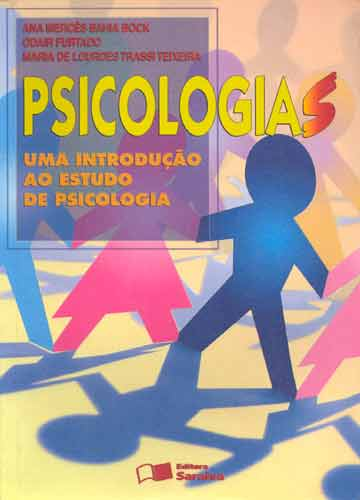
\includegraphics[width=0.5\linewidth]{figuras/LIVRO-PSICOLOGIAS-BOCH} 

}

\caption{Livro Psicologias: Uma Introdução ao Estudo da Psicologia. 13.ed. São Paulo: Saraiva, 2001}\label{fig:unnamed-chunk-17}
\end{figure}

\hypertarget{resumo-do-capuxedtulo-3---o-behaviorismo-1}{%
\subsection{Resumo do Capítulo 3 - O Behaviorismo}\label{resumo-do-capuxedtulo-3---o-behaviorismo-1}}

\begin{itemize}
\tightlist
\item
  Em breve, disponibilizaremos.
\end{itemize}

\hypertarget{resumo-do-capuxedtulo-4---a-gestalt-1}{%
\subsection{Resumo do Capítulo 4 - A Gestalt}\label{resumo-do-capuxedtulo-4---a-gestalt-1}}

\hypertarget{a-psicologia-da-forma-introduuxe7uxe3o-uxe0-psicologia-da-gestalt-1}{%
\subsection{A Psicologia da Forma: Introdução à Psicologia da Gestalt}\label{a-psicologia-da-forma-introduuxe7uxe3o-uxe0-psicologia-da-gestalt-1}}

\begin{itemize}
\tightlist
\item
  Para Bock (2001, p.~59) a Psicologia da Gestalt é uma das tendências teóricas mais \textbf{coerentes} e \textbf{coesas} da história da psicologia.
\item
  O termo Gestalt é de origem alemã e tem significado aproximado ao de \textbf{forma} ou \textbf{configuração}, porém \textbf{NÃO É UTILIZADO} por não corresponder exatamente as seu real significado em psicologia.
\item
  No final do século XIII, estudiosos procuravam compreender o \textbf{fenômeno psicológico} em seus aspectos naturais.

  \begin{itemize}
  \tightlist
  \item
    Principalmente no sentido da \textbf{mensurabilidade} ( A Psicofísica em voga ).
  \end{itemize}
\end{itemize}

\hypertarget{predecessores-da-psiologia-da-gestalt-1}{%
\subsection{Predecessores da Psiologia da Gestalt}\label{predecessores-da-psiologia-da-gestalt-1}}

\begin{itemize}
\tightlist
\item
  Estudiosos considerados os mais diretos predecessores/antecessores da Psisocologia Gestalt:

  \begin{itemize}
  \tightlist
  \item
    Ernst Mash (1838-1916), físico;
  \item
    Christian von Ehrenfels (1859-1932), fisólofo e psicólogo
  \end{itemize}
\item
  Estudos desenvolvidos:

  \begin{itemize}
  \tightlist
  \item
    Estudos psicofísicos sobre as \textbf{sensações} de \textbf{espaço-forma} e \textbf{tempo-forma}

    \begin{itemize}
    \tightlist
    \item
      Dado Psicológico: Sensações
    \item
      Dados Físico: espaço-forma e tempo-forma
    \end{itemize}
  \end{itemize}
\end{itemize}

\hypertarget{fundadores-da-psiologia-da-gestalt-1}{%
\subsection{Fundadores da Psiologia da Gestalt}\label{fundadores-da-psiologia-da-gestalt-1}}

\begin{itemize}
\tightlist
\item
  Os fundadores da Psicologia da Gestalt construíram a \textbf{base de uma teoria psicológica}.
\end{itemize}

\begin{figure}

{\centering 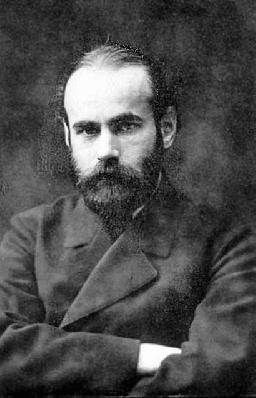
\includegraphics[width=0.3\linewidth]{figuras/MaxWertheimer} 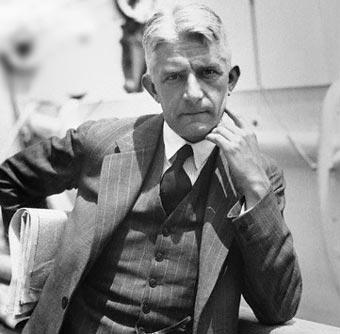
\includegraphics[width=0.3\linewidth]{figuras/WolfgangKohler} 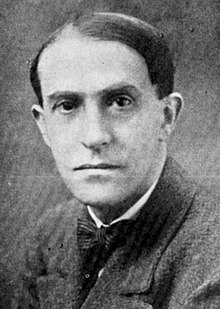
\includegraphics[width=0.3\linewidth]{figuras/KurtKoffka} 

}

\caption{Fundadores da Gestalt: Max Wertheimer | Wolfgang Kohler | Kurt Koffka}\label{fig:unnamed-chunk-18}
\end{figure}

\textbf{Obs}: Clique em :speaker: para ouvir a pronúncia dos nomes dos cientístas acima.

\begin{itemize}
\tightlist
\item
  Estudos iniciais

  \begin{itemize}
  \tightlist
  \item
    Estudos da percepção e sensação do movimento;
  \item
    Preocupação: Compreender \textbf{quais processos psicológicos} estavam envolvidos na \textbf{ilusão de ótica} quando o estímulo é percebido como uma \textbf{forma} diferente da que o sujeito tem na realidade.

    \begin{itemize}
    \tightlist
    \item
      Exemplo: Cinema; fotogramas estáticos; imagem formada na retina que demora um pouco para ser apagada; ilusão de óptica do movimento (sensação).
    \end{itemize}
  \end{itemize}
\end{itemize}

\hypertarget{a-percepuxe7uxe3o-1}{%
\subsection{A percepção}\label{a-percepuxe7uxe3o-1}}

\begin{itemize}
\tightlist
\item
  É \textbf{ponto de partida} e \textbf{tema central} da Psicologia da Gestalt;
\item
  Teoria Behaviorista

  \begin{itemize}
  \tightlist
  \item
    \textbf{Princípio Implícito}: Há uma relação de \textbf{causa} e \textbf{efeito} entre o \textbf{estímulo} e a \textbf{resposta}
  \end{itemize}
\item
  Para Gestaltistas há um questionamento desse \textbf{princípio implícito da teoria behaviorista}

  \begin{itemize}
  \tightlist
  \item
    Entre o \textbf{estímulo} e a \textbf{resposta} encontra-se o processo de percepção
  \item
    O QUE o indivíduo percebe e COMO o indivíduo percebe são importantes para entender o COMPORTAMENTO
  \end{itemize}
\end{itemize}

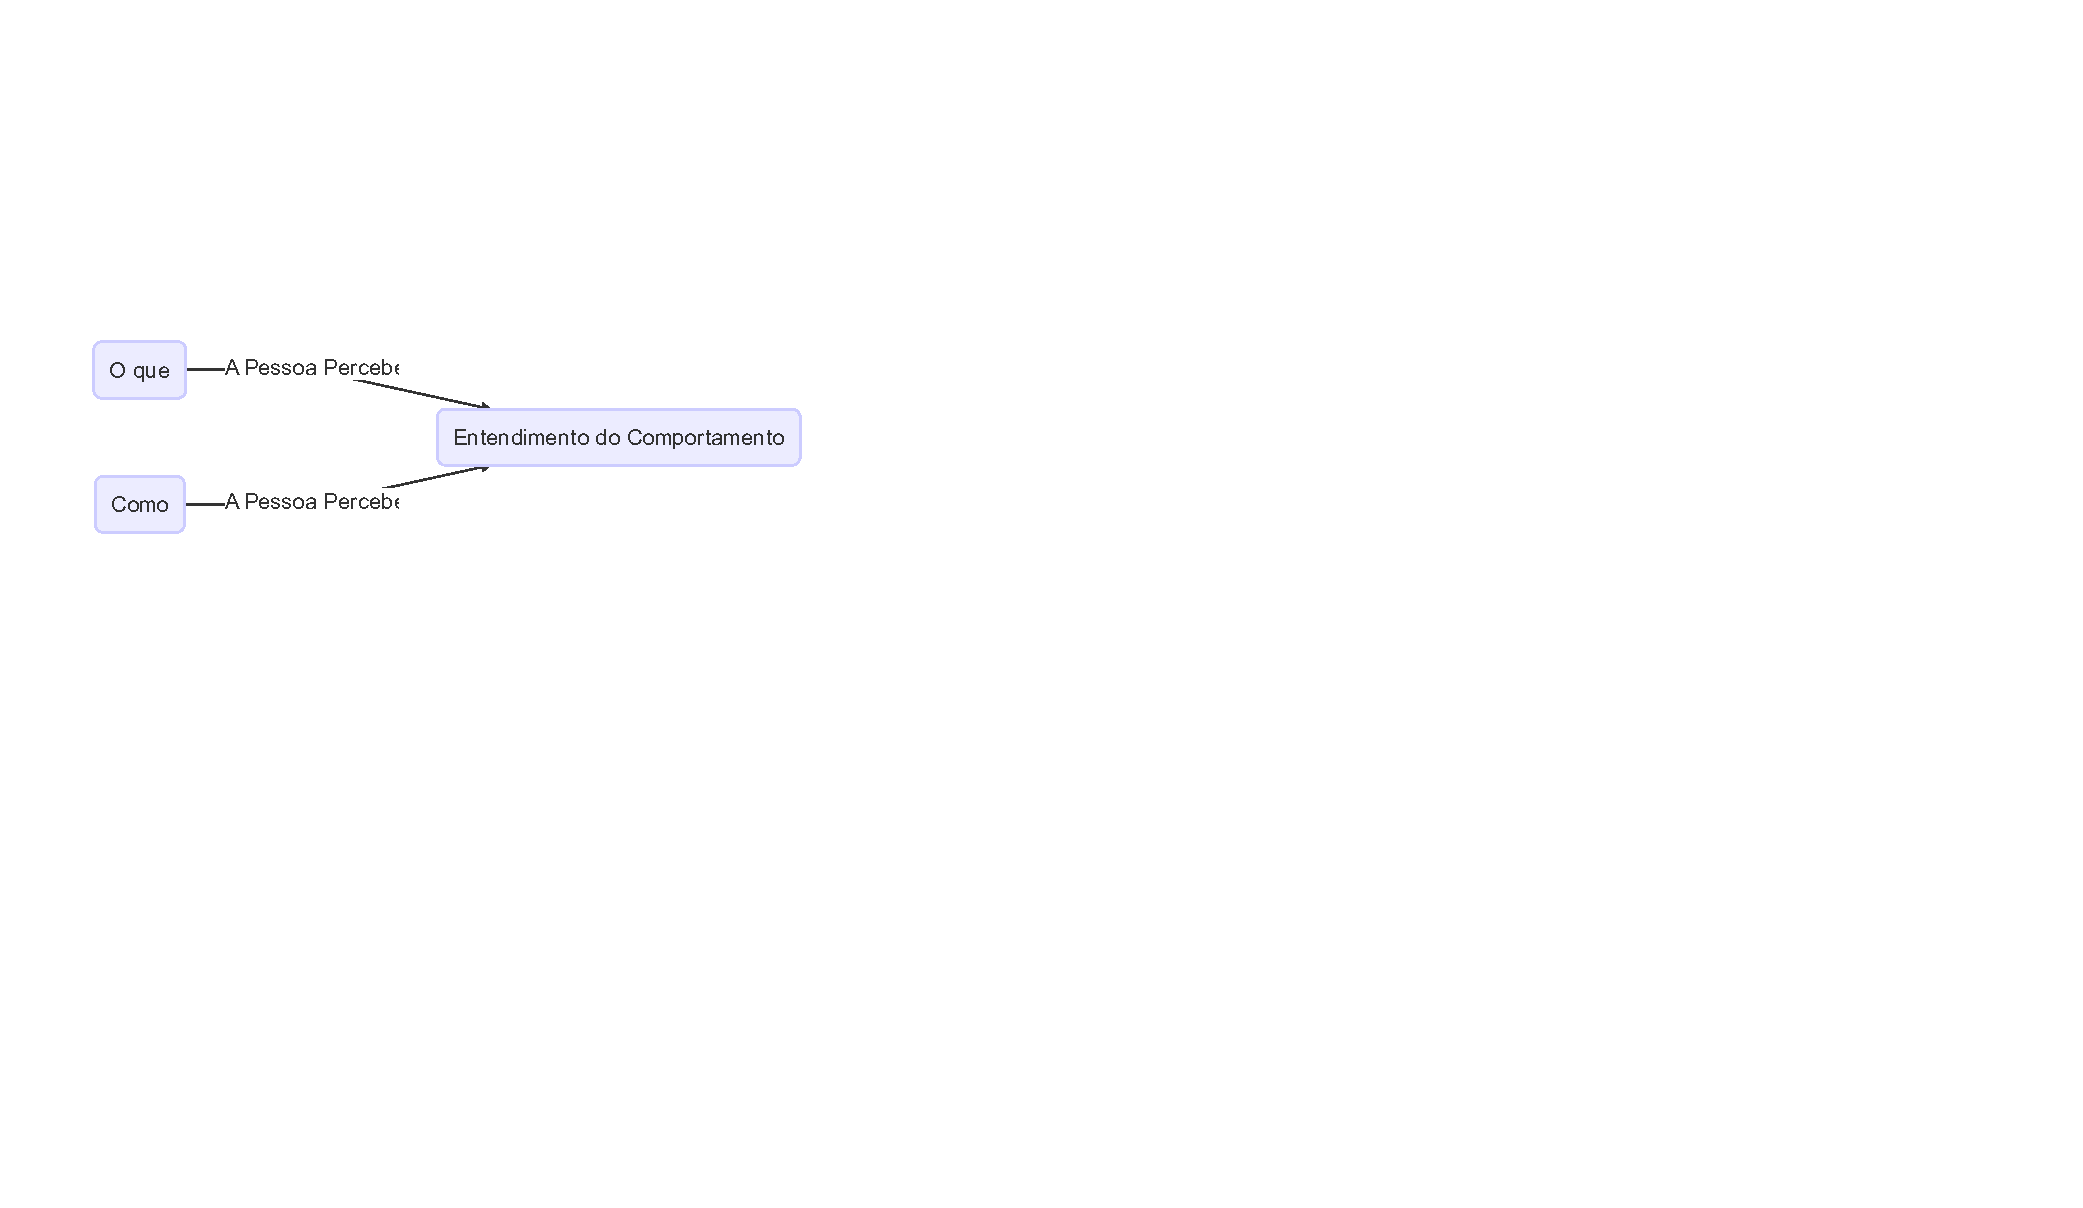
\includegraphics[width=1\linewidth]{Bookdown-Introducao-a-Psicologia_files/figure-latex/Entendimento do Comportamento 2-1}

\hypertarget{posiuxe7uxe3o-de-behavioristas-x-gestaltistas-diante-do-objeto-da-psicologia-1}{%
\subsection{Posição de Behavioristas x Gestaltistas diante do Objeto da Psicologia}\label{posiuxe7uxe3o-de-behavioristas-x-gestaltistas-diante-do-objeto-da-psicologia-1}}

\begin{itemize}
\tightlist
\item
  Ambos definem a psicologia como a ciência que estuda o COMPORTAMENTO
\item
  Para os Behavioristas:

  \begin{itemize}
  \tightlist
  \item
    É mais profunda a preocupação com a \textbf{objetividade};
  \item
    O \textbf{estudo com comportamento} é feito através da \textbf{relação estímulo-resposta};
  \item
    Despreza os conteúdos da consciência pela impossibilidade de controlar cientificamente \textbf{essas variáveis};
  \item
    Procura isolar o \textbf{estímulo} que corresponderia à \textbf{resposta} desprezando conteúdos da consciência pela impossibilidade de controlar cientificamente \textbf{essas variáveis};
  \end{itemize}
\item
  Para os gestaltistas:

  \begin{itemize}
  \tightlist
  \item
    Há uma \textbf{crítica} a \textbf{abordagem behaviorista} acima;
  \item
    Acreditam que existe um \textbf{contexto mais amplo} que é importante no \textbf{estudo do comportamento}

    \begin{itemize}
    \tightlist
    \item
      Esse \textbf{contexto mais amplo} são as CONDIÇÕES que \textbf{afetam/alteram} nossa capacidade de PERCEBER o \textbf{estímulo};
    \end{itemize}
  \item
    Entendem que estudar o comportamento isolado de um \textbf{contexto mais amplo} pode prejudicar o entendimento do comportamento pelo psicólogo;
  \item
    O comportamento é estudado em seus aspectos mais globais levando em consideração as CONDIÇÕES que \textbf{afetam/alteram} nossa capacidade de PERCEBER o \textbf{estímulo}
  \end{itemize}
\end{itemize}

\hypertarget{o-que-garante-o-entendimento-do-que-eu-percebo-1}{%
\subsection{O que Garante o Entendimento do que Eu Percebo ?}\label{o-que-garante-o-entendimento-do-que-eu-percebo-1}}

\begin{itemize}
\tightlist
\item
  Quando eu vejo

  \begin{itemize}
  \tightlist
  \item
    Uma parte de um objeto
  \end{itemize}
\item
  Ocorre uma tendência à

  \begin{itemize}
  \tightlist
  \item
    restauração do \textbf{equilíbrio da forma}
  \end{itemize}
\item
  Garantindo
  * O entendimento do que estou percebendo
\end{itemize}

\hypertarget{o-fenuxf4meno-da-percepuxe7uxe3o-1}{%
\subsection{O Fenômeno da Percepção}\label{o-fenuxf4meno-da-percepuxe7uxe3o-1}}

\begin{itemize}
\tightlist
\item
  É norteado pela busca de

  \begin{itemize}
  \tightlist
  \item
    \textbf{fechamento} dos pontos que compõem uma figura;
  \item
    \textbf{simetria} dos pontos que compõem uma figura;
  \item
    \textbf{regularidade} dos pontos que compõem uma figura;
  \end{itemize}
\item
  \textbf{Rudolf Arnheim} afirma que o \textbf{sentido normal da visão} apreende um \textbf{padrão global};
\end{itemize}

gestalt-Lei-basica-da-percepcao-visual.jpg

\begin{figure}

{\centering 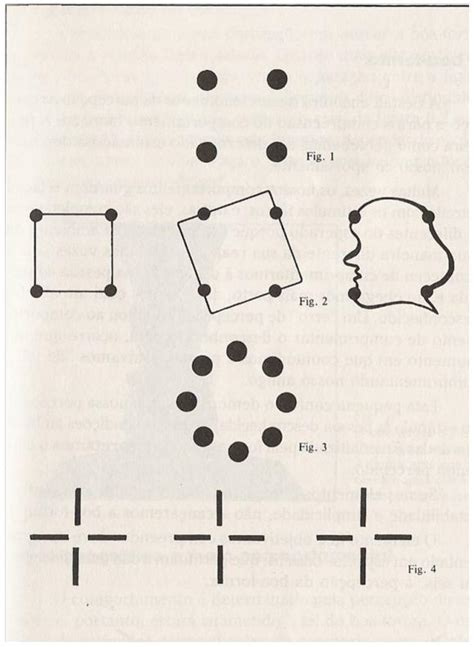
\includegraphics[width=0.6\linewidth]{figuras/gestalt-Lei-basica-da-percepcao-visual} 

}

\caption{Lei básica da percepção visual para os psicólogos da Gestalt}\label{fig:unnamed-chunk-19}
\end{figure}

\begin{itemize}
\tightlist
\item
  Observações a respeito da Figura:

  \begin{itemize}
  \tightlist
  \item
    \textbf{Figura 1}:

    \begin{itemize}
    \tightlist
    \item
      Percebemos como um \textbf{quadrado} e não como uma \textbf{figura inclinada} ou um \textbf{perfil} (Figura 2)
    \end{itemize}
  \item
    \textbf{Figura 3}:

    \begin{itemize}
    \tightlist
    \item
      Após acrescentarmos quatro pontos, o padrão percebido na Figura 1 irá mudar e perceberemos \textbf{um círculo}
    \end{itemize}
  \item
    \textbf{Figura 4}:

    \begin{itemize}
    \tightlist
    \item
      É possível ver tanto \textbf{círculos brancos} quanto \textbf{quadrados brancos} nos centros das cruzes;
    \end{itemize}
  \end{itemize}
\end{itemize}

\begin{quote}
Qualquer padrão de estímulo tende a ser visto de tal modo que a \textbf{estrutura resultante} é tão \textbf{simples} quanto as \textbf{condições dadas} permitem
\end{quote}

\hypertarget{a-boa-forma-1}{%
\subsection{A boa-forma}\label{a-boa-forma-1}}

\begin{itemize}
\tightlist
\item
  A Psicologia da Gestalt encontra as \textbf{condições} para a \textbf{compreensão do comportamento humano} nos \textbf{fenômenos da percepção}.
\item
  Em relação aos nossos comportamentos:

  \begin{itemize}
  \tightlist
  \item
    Em alguns casos, \textbf{guardam estreita relação com os estímulos físicos};
  \item
    Em outros casos, \textbf{são completamente diferentes do esperado} porque ``entendemos o ambiente'' \textbf{de maneira diferente da sua realidade}.
  \item
    Exemplo:

    \begin{itemize}
    \tightlist
    \item
      Cumprimentar uma pessoas e depois descobrir que cumprimentamos uma pessoa desconhecida (\textbf{Erro de Percepção});
    \end{itemize}
  \end{itemize}
\item
  Não há \textbf{boa forma} quando \textbf{nos elementos percebidos} não há:

  \begin{itemize}
  \tightlist
  \item
    Equilíbrio
  \item
    Simetria
  \item
    Estabilidade
  \item
    Simplicidade
  \end{itemize}
\item
  \textbf{O elemento que objetivamos compreender}

  \begin{itemize}
  \tightlist
  \item
    COMO DEVE SER APRESENTADO

    \begin{itemize}
    \tightlist
    \item
      Deve ser apresentado em \textbf{aspectos básicos} que \textbf{permitam a sua decodificação} (\textbf{percepção da boa forma})
    \end{itemize}
  \end{itemize}
\end{itemize}

\begin{figure}

{\centering 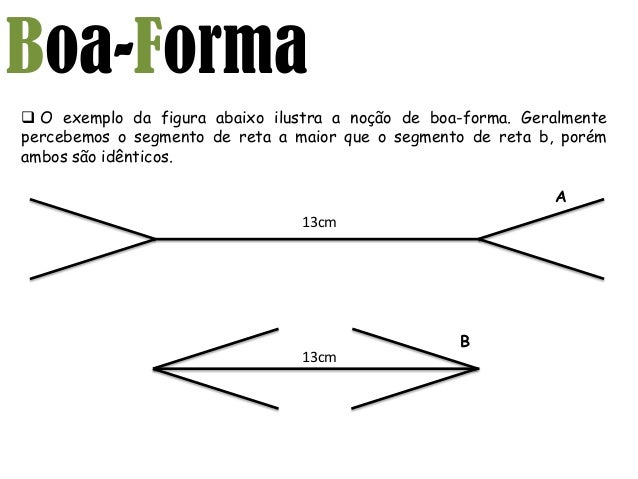
\includegraphics[width=0.7\linewidth]{figuras/gestalt-exemplo-boa-forma} 

}

\caption{Observe a RETA: Elemento que desejamos compreender}\label{fig:unnamed-chunk-20}
\end{figure}

\begin{itemize}
\tightlist
\item
  (\ldots)

  \begin{itemize}
  \tightlist
  \item
    COMO DEVEM SER DISTRIBUÍDOS OS ELEMENTOS QUE O COMPÕEM
    * Para garantir a \textbf{boa forma} devem ser apresentados com
    * Equilíbrio
    * Simetria
    * Estabilidade
    * Simplicidade
  \end{itemize}
\item
  A \textbf{tendência da nossa percepção} em buscar a \textbf{boa forma} permitirá a relação \textbf{figura-fundo}
\item
  Quanto mais clara (simples, estável, simétrica e equilibrada) estiver a \textbf{boa-forma}

  \begin{itemize}
  \tightlist
  \item
    Mais clara será a \textbf{separação} entre \textbf{figura} e \textbf{fundo};
  \end{itemize}
\item
  Quanto menos clara estiver a boa forma

  \begin{itemize}
  \tightlist
  \item
    Mais difícil será distinguir o que é figura e o que é fundo (Figura Ambígua);
  \end{itemize}
\end{itemize}

\hypertarget{meio-geogruxe1fico-e-meio-comportamental-1}{%
\subsection{Meio Geográfico e Meio Comportamental}\label{meio-geogruxe1fico-e-meio-comportamental-1}}

\begin{itemize}
\tightlist
\item
  O comportamento \textbf{É DETERMINADO} pela \textbf{PERCEPÇÃO DO ESTÍMULO};
\item
  O comportamento está/estará sujeito a \textbf{LEI DA BOA-FORMA};
\item
  O \textbf{CONJUNTO DE ESTÍMULOS} determinantes do comportamento é denominado \textbf{MEIO AMBIENTAL} ( ou apenas MEIO )
\item
  Existem DOIS TIPOS DE MEIOS AMBIENTAIS

  \begin{itemize}
  \tightlist
  \item
    \textbf{Meio GEOGRÁFICO}

    \begin{itemize}
    \tightlist
    \item
      É o meio enquanto tal;
    \item
      É o meio físico EM TERMOS OBJETIVOS;
    \end{itemize}
  \item
    \textbf{Meio COMPORTAMENTAL}

    \begin{itemize}
    \tightlist
    \item
      É o meio resultante de INTERAÇÃO (Indivíduo ⇔ Meio Físico)
    \item
      Implica a \textbf{INTERPRETAÇÃO} desse meio através das \textbf{FORÇAS} que regem a \textbf{PERCEPÇÃO};

      \begin{itemize}
      \tightlist
      \item
        Forças que regem a percepção:

        \begin{itemize}
        \tightlist
        \item
          Equilíbrio
        \item
          Simetria
        \item
          Estabilidade
        \item
          Simplicidade
        \end{itemize}
      \end{itemize}
    \end{itemize}
  \end{itemize}
\item
  Exemplo

  \begin{itemize}
  \tightlist
  \item
    Cumprimentar uma pessoa desconhecida
  \item
    Se só tivéssemos o \textbf{MEIO GEOGRÁFICO}, essa seria a nossa ÚNICA POSSIBILIDADE de percepção;
  \item
    A \textbf{SITUAÇÃO} levou-nos a uma \textbf{INTERPRETAÇÃO DIFERENTE DA REALIDADE} e ocorre a confusão com uma pessoa conhecida

    \begin{itemize}
    \tightlist
    \item
      DADOS DA SITUAÇÃO:

      \begin{itemize}
      \tightlist
      \item
        Encontro casual
      \item
        Encontro em movimento
      \item
        Impulso em manifestar uma reação ao encontro
      \end{itemize}
    \end{itemize}
  \item
    No caso desse exemplo

    \begin{itemize}
    \tightlist
    \item
      A semelhança entre as duas pessoas foi \textbf{A CAUSA DO ENGANO(=COMPORTAMENTO)}
    \item
      Houve uma tendência em ESTABELECER A UNIDADE DE SEMELHANÇAS entre as duas pessoas, MAIS QUE SUAS DIFERÊNÇAS.
    \end{itemize}
  \end{itemize}
\item
  Essa \textbf{TENDÊNCIA A ``JUNTAR'' OS ELEMENTOS} é o que a Gestalt denomina de \textbf{FORÇA DE CAMPO PSICOLÓGICO;}
\item
  Nessa \textbf{PARTICULAR INTERPRETAÇÃO DO MEIO} (= O MEIO AMBIENTAL)

  \begin{itemize}
  \tightlist
  \item
    O que PERCEBEMOS é ``UMA REALIDADE'':

    \begin{itemize}
    \tightlist
    \item
      Realidade \textbf{PARTICULAR}
    \item
      Realidade \textbf{OBJETIVA}
    \item
      Realidade \textbf{CRIADA POR NOSSA MENTE}
    \end{itemize}
  \end{itemize}
\end{itemize}

\hypertarget{campo-psicoluxf3gico-1}{%
\subsection{Campo Psicológico}\label{campo-psicoluxf3gico-1}}

\begin{itemize}
\tightlist
\item
  Campo psicológico é uma tendência que \textbf{garante} (1) a busca pela melhor forma possível \textbf{em situações que não estão muito claras}.
\end{itemize}

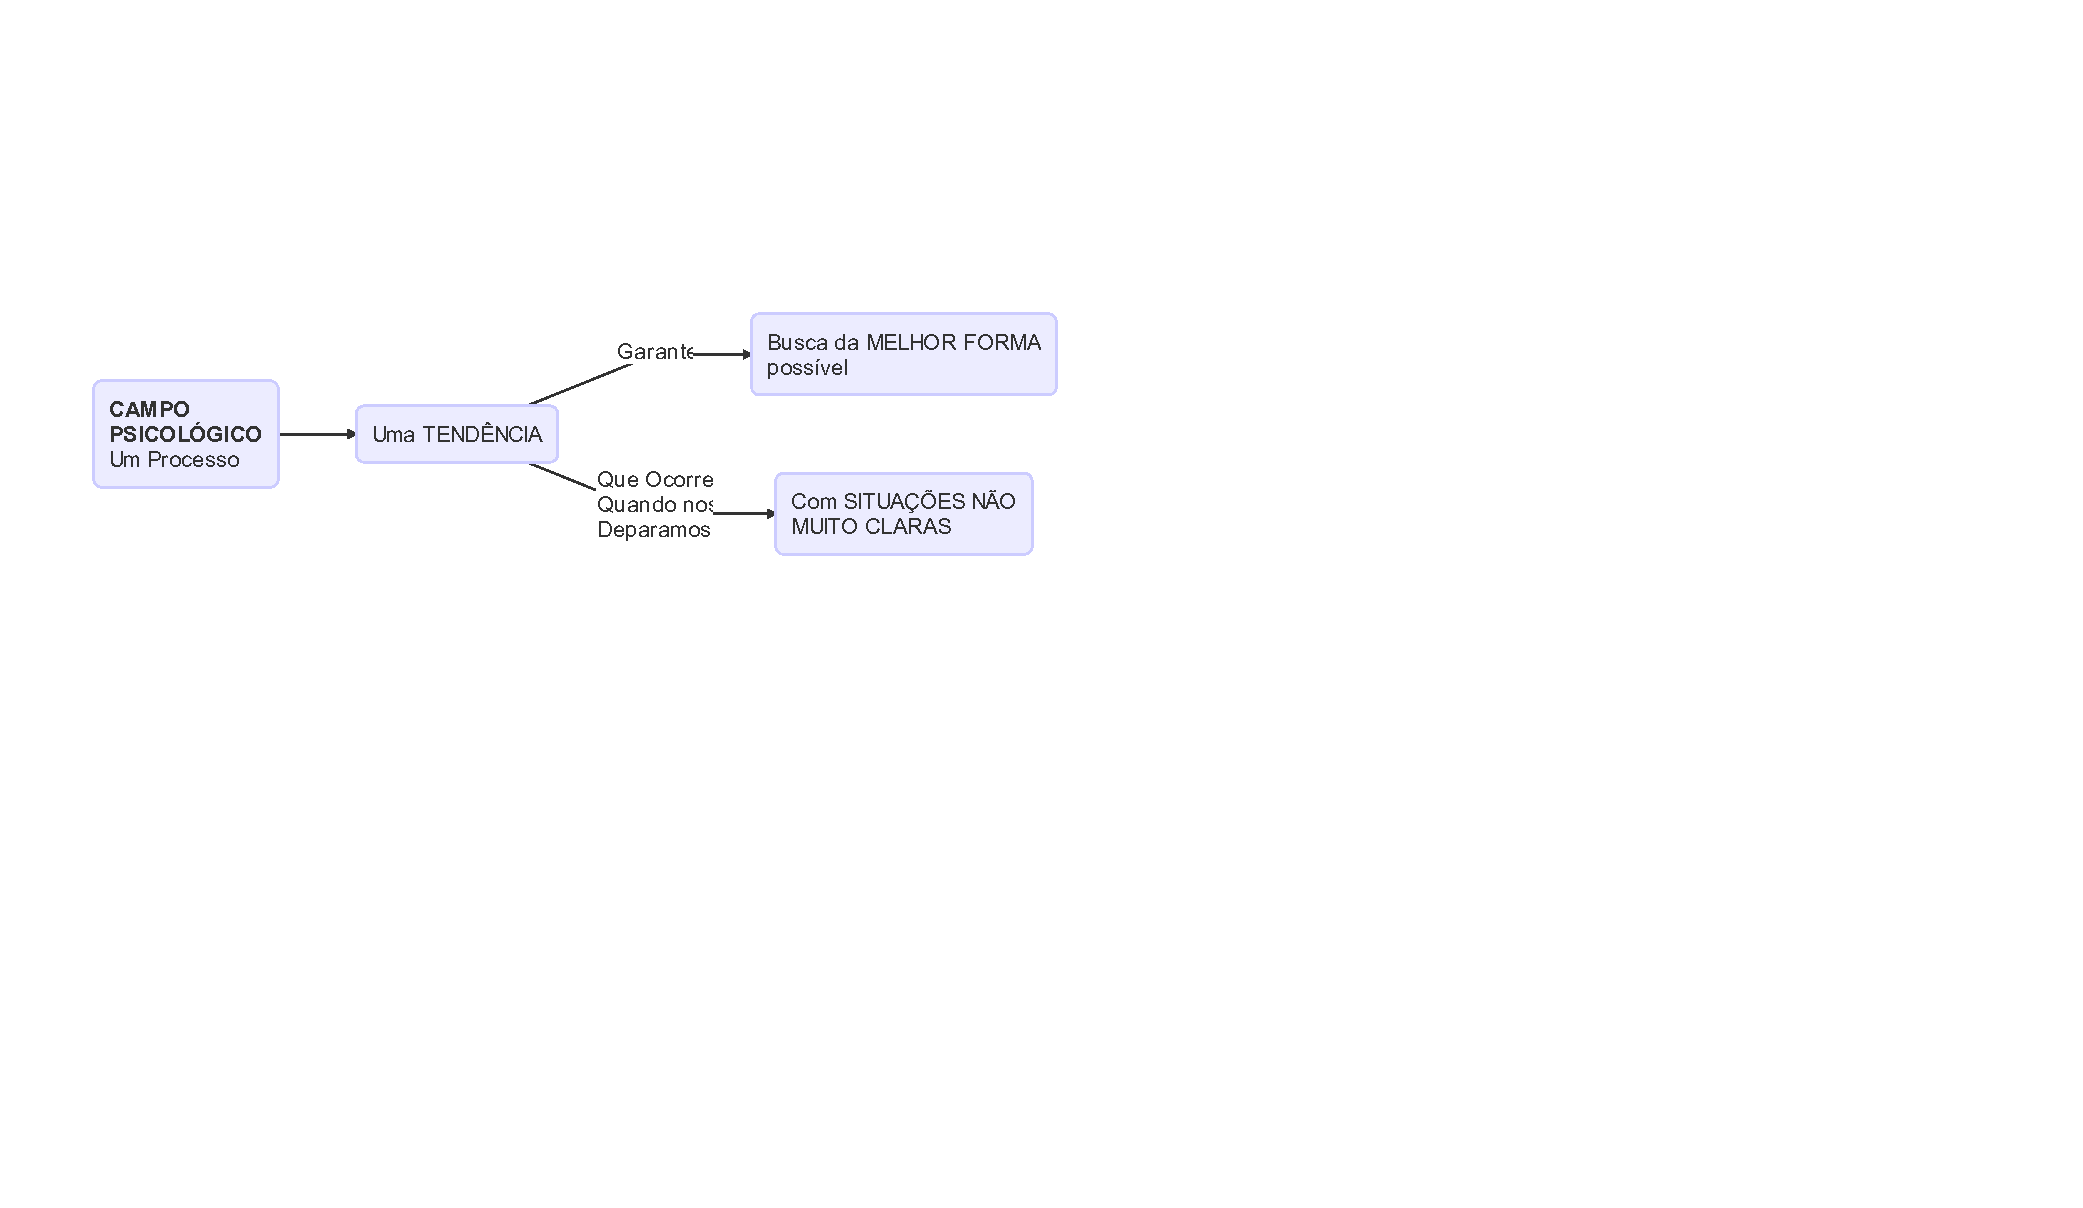
\includegraphics[width=1\linewidth]{Bookdown-Introducao-a-Psicologia_files/figure-latex/Campo Psicologico-1}

\hypertarget{princuxedpios-do-campo-psicoluxf3gico-1}{%
\subsection{Princípios do Campo Psicológico}\label{princuxedpios-do-campo-psicoluxf3gico-1}}

\begin{itemize}
\tightlist
\item
  O campo psicológico é um processo que ocorre de acordo com \textbf{PRINCÍPIOS}:
\end{itemize}

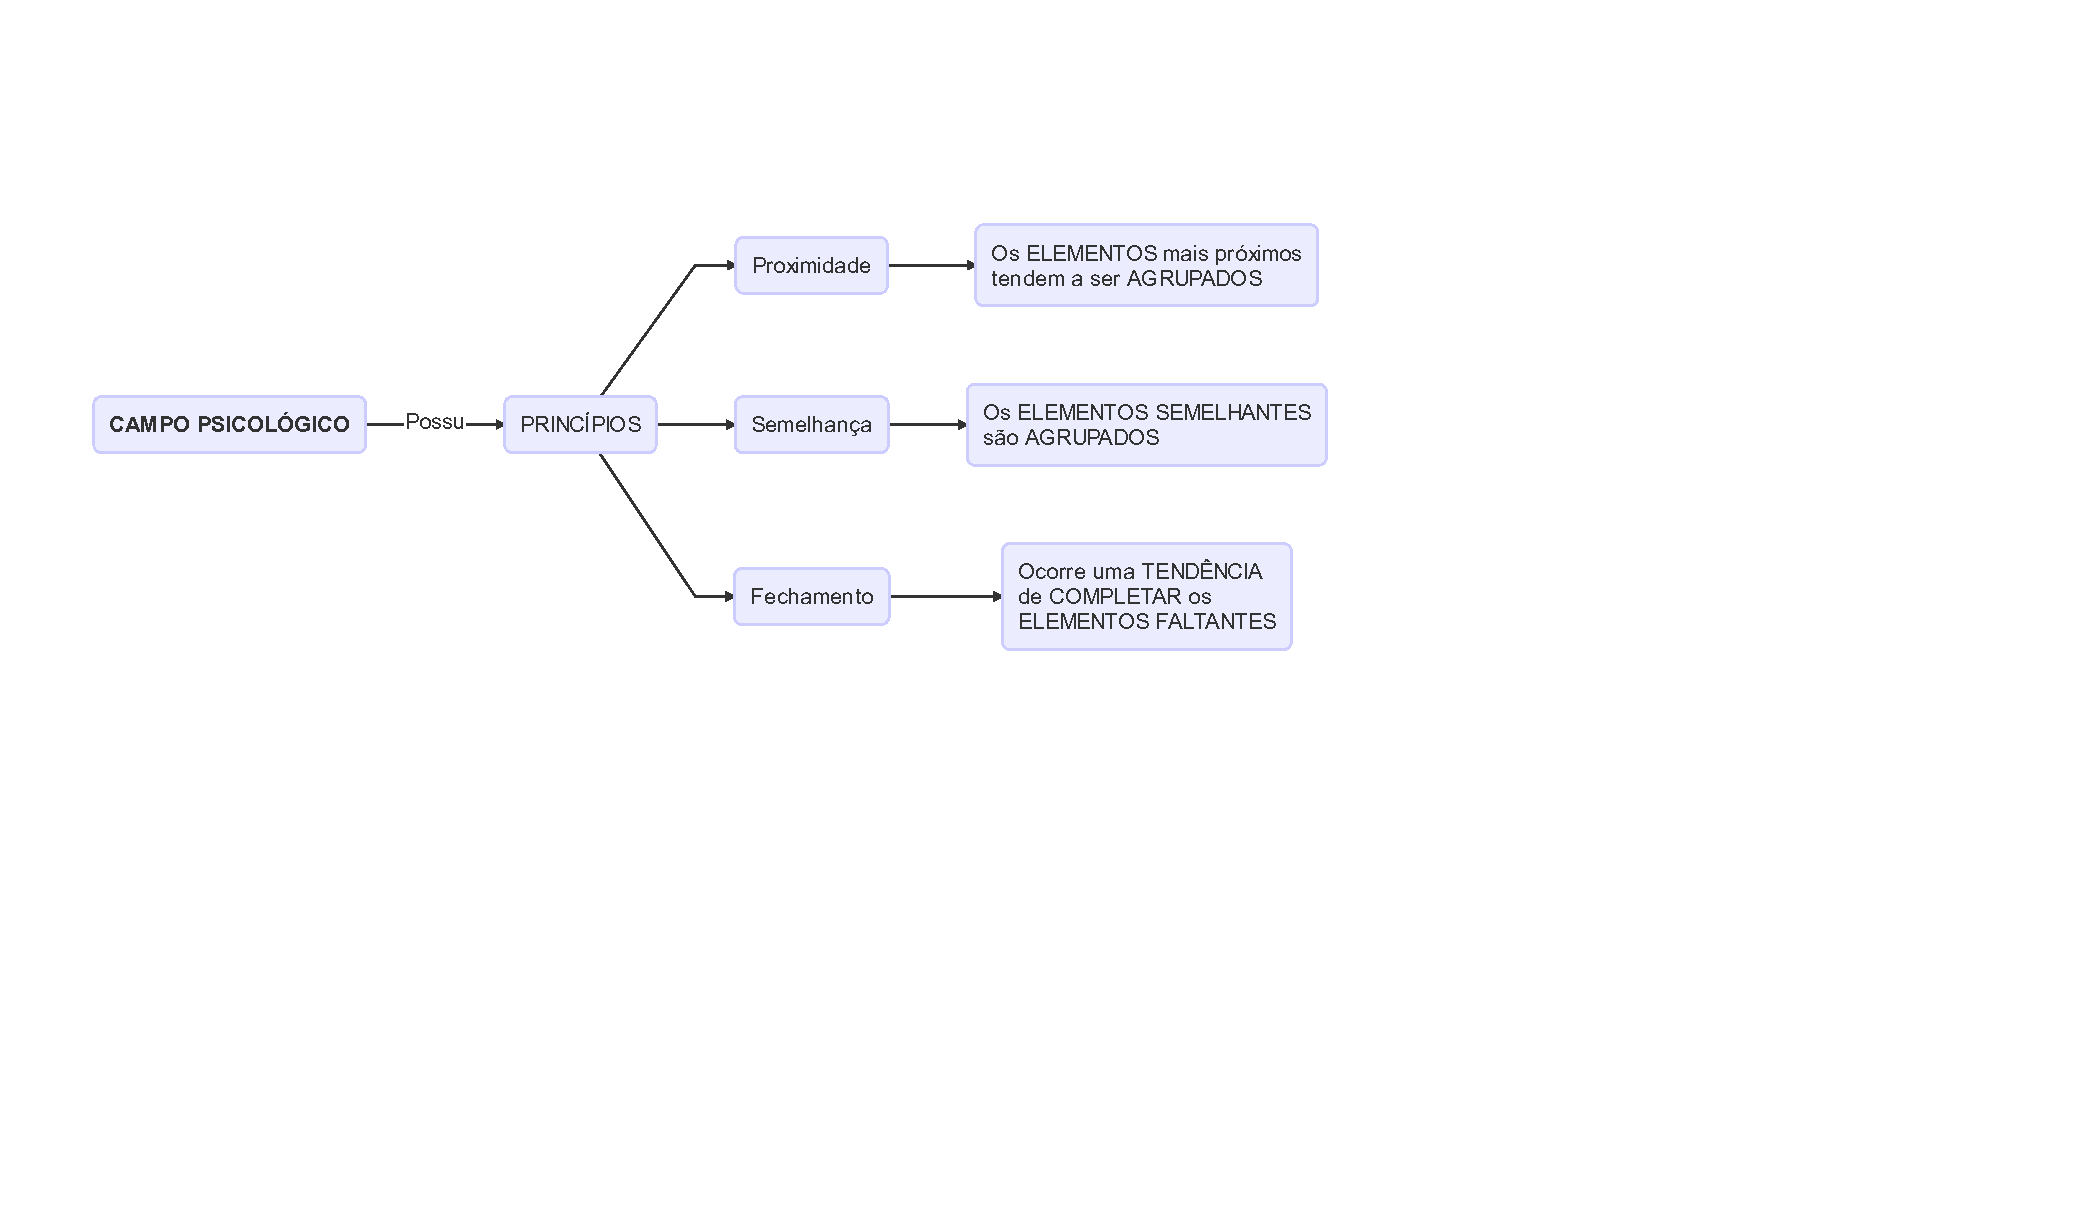
\includegraphics[width=1\linewidth]{Bookdown-Introducao-a-Psicologia_files/figure-latex/Principios do Campo Psicologico-1}

\hypertarget{insight-1}{%
\subsection{Insight}\label{insight-1}}

\begin{itemize}
\tightlist
\item
  Significa \textbf{COMPREENSÃO IMEDIATA};
\item
  Existe uma diferença em como duas correntes psicológicas concebem o *\textbf{processo de aprendizagem}:

  \begin{itemize}
  \tightlist
  \item
    \textbf{A Gestalt}

    \begin{itemize}
    \tightlist
    \item
      Acredita que a APRENDIZAGEM é uma RELAÇÃO entre o TODO e a PARTE;
    \end{itemize}
  \item
    \textbf{O Associativismo / Behaviorismo}

    \begin{itemize}
    \tightlist
    \item
      Acredita que a APRENDIZAGEM é uma relação de coisas MAIS SIMPLES para coisas MAIS COMPLEXAS;
    \end{itemize}
  \end{itemize}
\item
  Na perspectiva da Geltalt, a APRENDIZAGEM é uma relação entre o TODO e a PARTE

  \begin{itemize}
  \tightlist
  \item
    Exemplo: É possível uma criança de 03 anos, que não sabe ler, distinguir a marca de um refrigerante e nomeá-lo corretamente.

    \begin{itemize}
    \tightlist
    \item
      Ela identificou e SEPAROU a PALAVA em sua TOTALIDADE, distinguindo a PALAVRA(figura) e o FUNDO;
    \item
      A criança aprendeu a ler a PALAVRA não juntando as letras, mas DANDO SIGNIFICADO ao TODO;
    \end{itemize}
  \end{itemize}
\item
  Nem sempre \textbf{AS SITUAÇÕES VIVIDAS} se apresentam DE FORMA CLARA de maneira a permitir uma PERCEPÇÃO IMEDIATA.

  \begin{itemize}
  \tightlist
  \item
    Essas situações DIFICULTAM O PROCESSO DE APRENDIZADO, porque não permitem uma clara definição da FIGURA-FUNDO, impedindo a relação PARTE/TODO
  \end{itemize}
\end{itemize}

\hypertarget{explicauxe7uxe3o-do-fenuxf4meno-de-insight-1}{%
\subsection{Explicação do Fenômeno de INSIGHT}\label{explicauxe7uxe3o-do-fenuxf4meno-de-insight-1}}

\begin{itemize}
\tightlist
\item
  Às vezes, estamos olhando para um \textbf{FIGURA} que \textbf{não tem sentido para nós}
\item
  De repente, sem que tenhamos feito nenhum esforço especial, \textbf{A RELAÇÃO FIGURA-FUNDOSE ESTABELECE}.
\end{itemize}

\hypertarget{teoria-de-campo-de-kurt-lewin-1}{%
\subsection{\texorpdfstring{Teoria de Campo de \textbf{Kurt Lewin}}{Teoria de Campo de Kurt Lewin}}\label{teoria-de-campo-de-kurt-lewin-1}}

\begin{figure}

{\centering 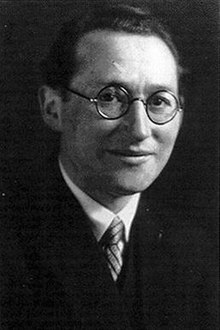
\includegraphics[width=0.4\linewidth]{figuras/KurtLewin} 

}

\caption{Kurt Lewin (1890-1947)}\label{fig:unnamed-chunk-21}
\end{figure}

\hypertarget{kurt-lewin-1890-1947-1}{%
\subsection{Kurt Lewin (1890-1947)}\label{kurt-lewin-1890-1947-1}}

\begin{itemize}
\tightlist
\item
  Foi um psicólogo germano-estadunidense pioneiro da Psicologia Aplicada, Social e Organizacional nos Estados Unidos*.
\item
  Trabalhou 10 anos com os pioneiros da Gestalt: Max Wertheimer, Wolfgang Kohler e Kurt Koffka
\item
  Não era um Gestaltista, apesar dessa colaboração, já que ele seguiu um caminho teórico diferente desses pioneiros
\item
  Da colaboração com os pioneiros da Gestalt nasceu a \textbf{Teoria de Campo}
\item
  Lewin partiu da \textbf{teoria da Gestalt} para construir novos conhecimentos para a psicologia.

  \begin{itemize}
  \tightlist
  \item
    Ele abandonou a preocupação \textbf{psicofisiológica}
  \item
    Ele buscou na \textbf{Física} a base metodológica de sua psicologia.
  \end{itemize}
\end{itemize}

\hypertarget{o-conceito-de-espauxe7o-vital-e-de-campo-psicoluxf3gico-de-lewin-1}{%
\subsection{\texorpdfstring{O Conceito de \textbf{Espaço Vital} e de \textbf{Campo Psicológico} de Lewin}{O Conceito de Espaço Vital e de Campo Psicológico de Lewin}}\label{o-conceito-de-espauxe7o-vital-e-de-campo-psicoluxf3gico-de-lewin-1}}

CAMPO VITAL

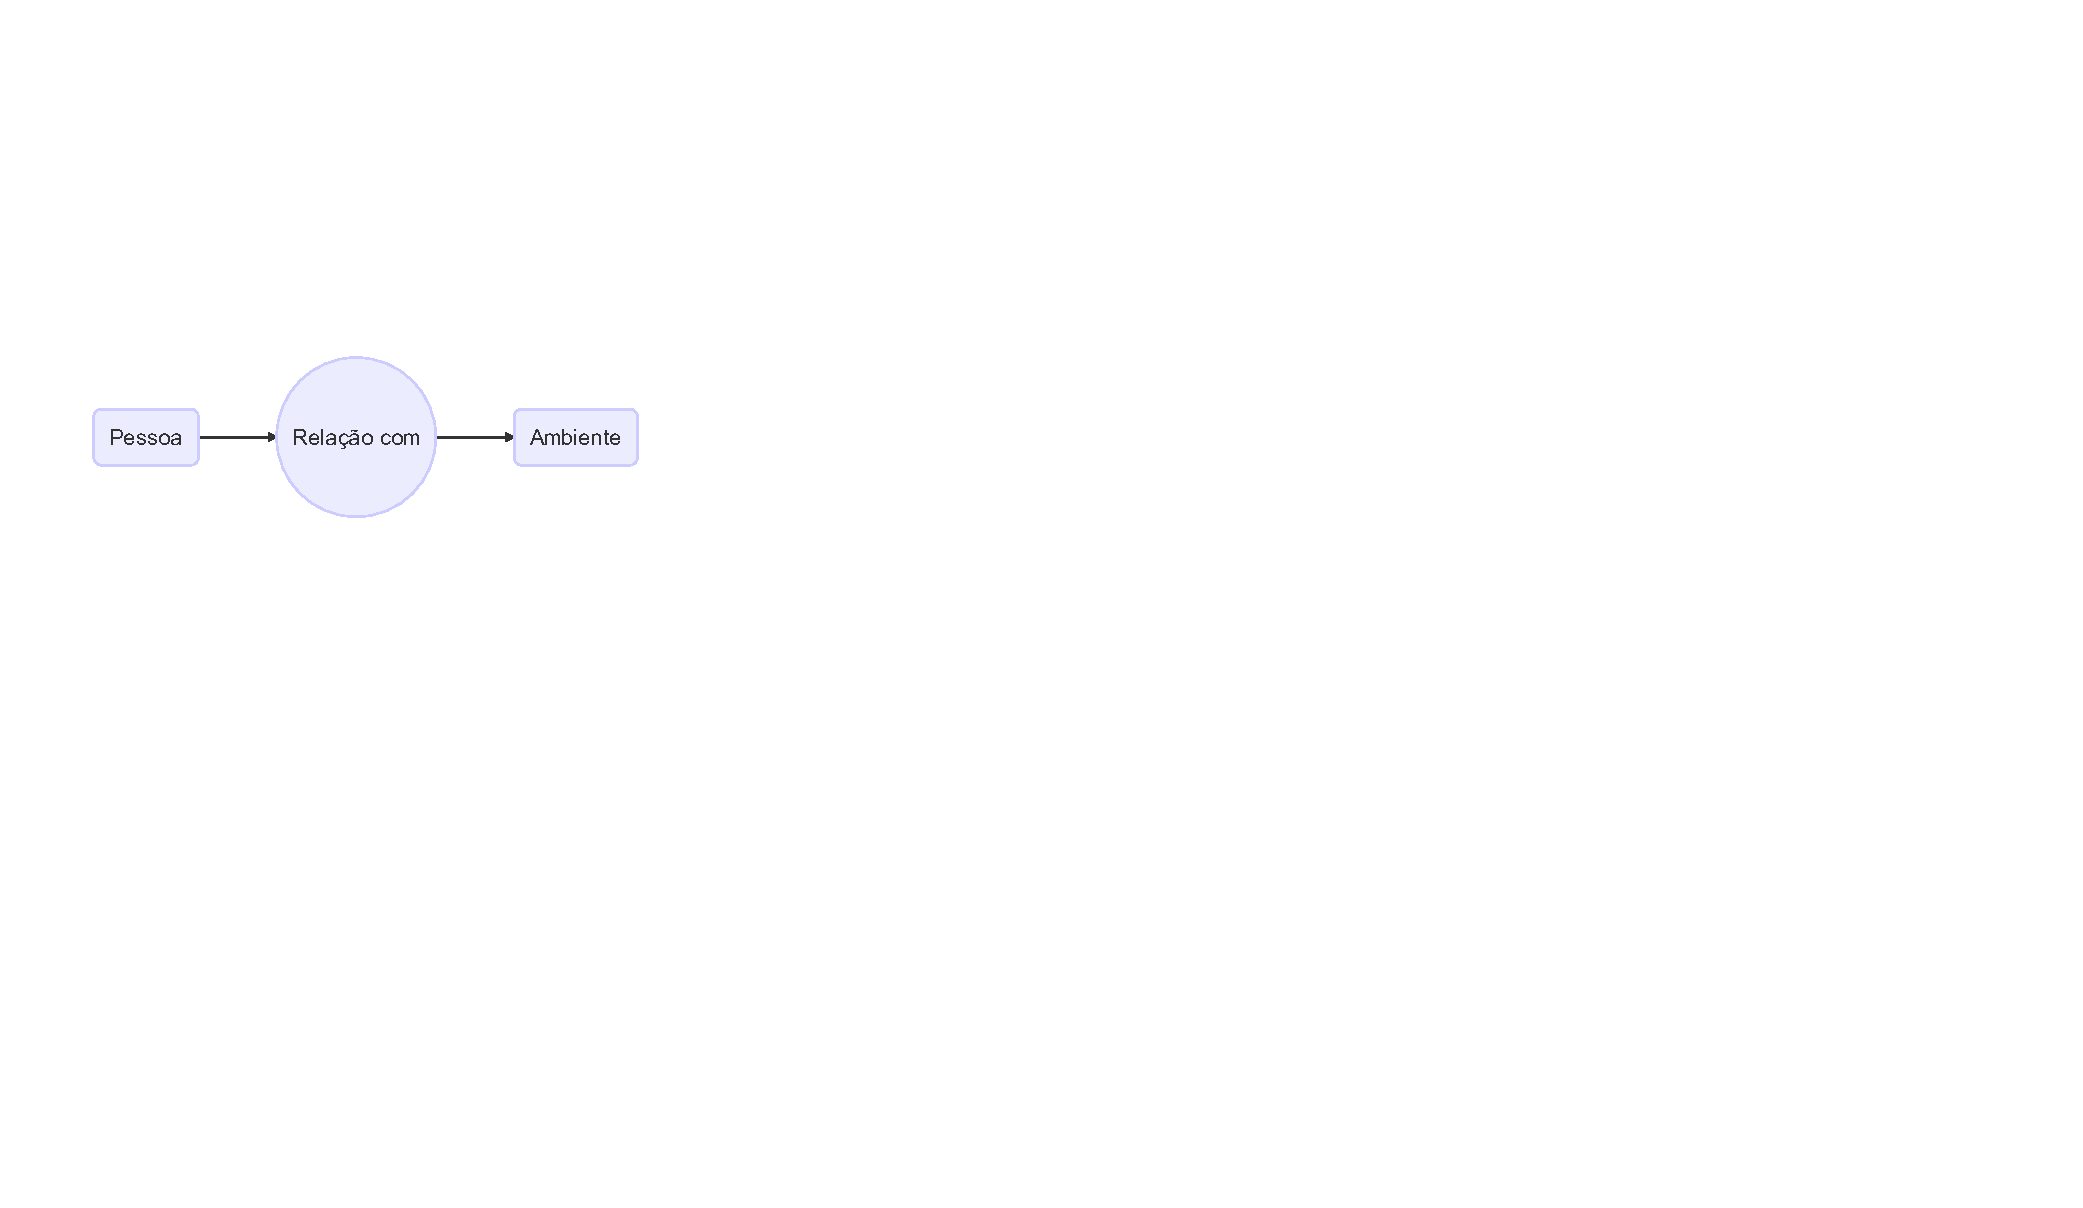
\includegraphics[width=1\linewidth]{Bookdown-Introducao-a-Psicologia_files/figure-latex/Campo Vital-1}

\begin{itemize}
\tightlist
\item
  A \textbf{DEFINIÇÃO} de \textbf{ESPAÇO VITAL}: ``A \textbf{totalidade dos fatos} que DETERMINAM O COMPORTAMENTO do indivíduo, num certo momento''.
\item
  Outro conceito definido por Lewin foi o de \textbf{campo psicológico}: ``É o espaço vital considerado dinamicamente'' que deve ser considerado (1)tal como ele se apresenta para o indivíduo, (2)em um determinado momento.

  \begin{itemize}
  \tightlist
  \item
    Leva-se em conta:

    \begin{itemize}
    \tightlist
    \item
      O indivíduo
    \item
      O meio
    \item
      A \textbf{totalidade dos fatos} coexistentes e mutuamente interdependentes
    \end{itemize}
  \end{itemize}
\item
  O CAMPO PSICOLÓGICO \textbf{NÃO É} uma \textbf{realidade física}.
\item
  O CAMPO PSICOLÓGICO \textbf{É} uma \textbf{realidade fenomênica}.
\item
  Para Lewin, \textbf{NÃO SÃO APENAS} fatos físicos que produzem efetos sobre o \textbf{comportamento}
\item
  O CAMPO PSICOLÓGICO deve ser representado:

  \begin{itemize}
  \tightlist
  \item
    \textbf{(1) tal como ele existe para o indivíduo},
  \item
    \textbf{(2) num determinado momento}.
  \item
    Ele não existe de forma isolada e estática ( ``\ldots{} e não como ele é em si.'').
  \end{itemize}
\item
  São \textbf{ESSENCIAIS} para CONSTRUÇÃO DO CAMPO PSICOLÓGICO:

  \begin{itemize}
  \tightlist
  \item
    Os objetivos CONSCIENTES;
  \item
    Os objetivos INCONSCIENTES;
  \item
    Os sonhos;
  \item
    Os medos;
  \item
    As amizades;
  \item
    O AMBIENTE FÍSICO;
  \end{itemize}
\end{itemize}

\hypertarget{a-realidade-fenomuxeanica-em-kurt-lewin-1}{%
\subsection{A REALIDADE FENOMÊNICA EM KURT LEWIN}\label{a-realidade-fenomuxeanica-em-kurt-lewin-1}}

O que é essa realidade fenomênica ?

\begin{enumerate}
\def\labelenumi{\arabic{enumi}.}
\tightlist
\item
  \textbf{A MANEIRA PARTICULAR COMO UM INDIVÍDUO INTERPRETA DETERMINADA SITUAÇÃO ➥ MEIO COMPORTAMENTAL da GESTALT}

  \begin{itemize}
  \tightlist
  \item
    \textbf{Obs}: ``A maneira particular como um indivíduo \textbf{INTERPRETA}'' significa a maneira como cada indivíduo \textbf{PERCEBE} enquanto fenômeno psicofisiológico
  \end{itemize}
\item
  As \textbf{CARACTERÍSTICAS DE PERSONALIDADE} do indivíduo;
\item
  Os \textbf{COMPONENTES EMOCIONAIS} ligados à situação \textbf{de vida} e \textbf{vivida} própria do indivíduo;
\item
  Os \textbf{COMPONENTES EMOCIONAIS} ligados \textbf{ao grupo} ao qual o indivíduo pertence;
\item
  As \textbf{SITUAÇÕES PASSADAS} que estejam ligadas ao acontecimento
\end{enumerate}

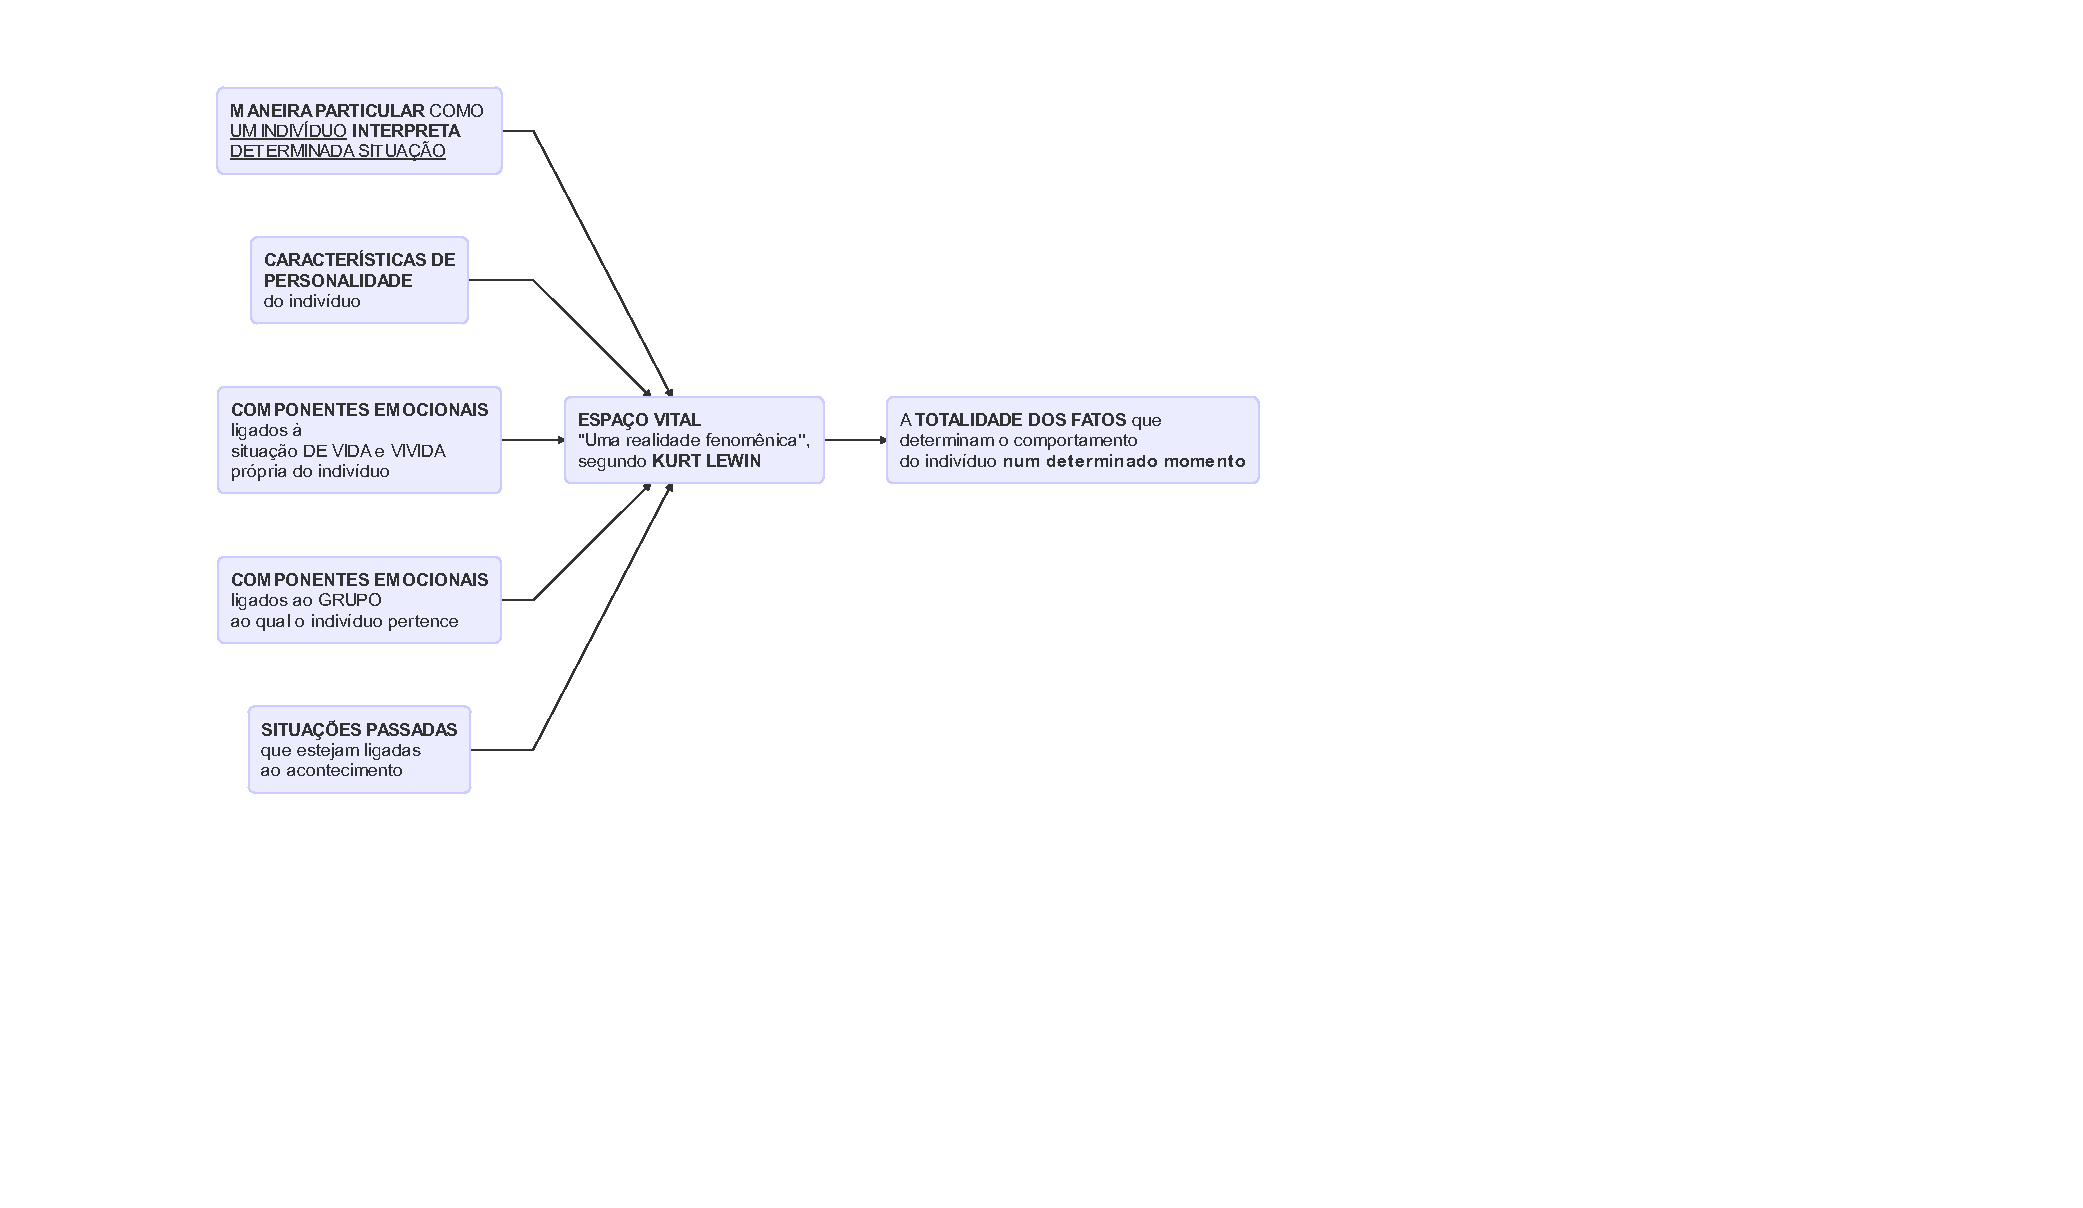
\includegraphics[width=1\linewidth]{Bookdown-Introducao-a-Psicologia_files/figure-latex/Realidade Fenomenica de Kurt Lewin-1}

\hypertarget{exemplo-campo-psicoluxf3gico-e-espauxe7o-vital-1}{%
\subsection{EXEMPLO: Campo Psicológico e Espaço Vital}\label{exemplo-campo-psicoluxf3gico-e-espauxe7o-vital-1}}

\begin{enumerate}
\def\labelenumi{\arabic{enumi}.}
\tightlist
\item
  \textbf{RELATO}:
\end{enumerate}

\begin{quote}
Um rapaz, ao chegar a sua casa, surpreende os pais num final de conversa e escuta o seguinte: ``Ele chegou, é melhor não falarmos disso agora''. \textbf{Ele entende que} OS PAIS CONVERSAVAM SOBRE UM \textbf{ASSUNTO SÉRIO}, de que \textbf{ele não deveria tomar conhecimento}. \textbf{RESOLVE não fazer nenhum comentário sobre o assunto}. Dias depois, chegando novamente em casa, encontra seus pais na sala com dois homens em ternos escuros. Imediatamente, associa esses homens ao final da conversa escutada e entende que eles, de alguma forma, estariam relacionados às preocupações dos pais.
\end{quote}

\begin{enumerate}
\def\labelenumi{\arabic{enumi}.}
\setcounter{enumi}{1}
\tightlist
\item
  \textbf{COMPORTAMENTO DETERMINADO PELO CAMPO PCISOLÓGICO}:
\end{enumerate}

\begin{itemize}
\tightlist
\item
  ``\textbf{RESOLVE} não fazer comentários sobre o assunto'';
\item
  Ele procurou ``\textbf{fingir que não havia escutado}'';
\end{itemize}

\begin{enumerate}
\def\labelenumi{\arabic{enumi}.}
\setcounter{enumi}{2}
\tightlist
\item
  \textbf{CONSIDERAÇÕES:}
\end{enumerate}

\begin{itemize}
\tightlist
\item
  Nessa estória, o \textbf{CAMPO PSICOLÓGICO} é representado pelas \textbf{``linhas de força''} que \textbf{(1/2)atraem a percepção} e \textbf{(2/2)lhe dão significado};
\item
  O rapaz (indivíduo) interpretou a situação pelo seu \textbf{ASPECTO FENOMÊNICO} e não pelo que ocorria de fato;
\item
  A INTERPRETAÇÃO ganhou CONSISTÊNCIA com a visita de duas pessoas que ele não conhecia (TOTALIDADE DOS FATOS). Isso foi possível porque o rapaz havia MEMORIZADO A SITUAÇÃO ANTERIOR e a ela ASSOCIADO A SITUAÇÃO SEGUINTE (a nova situações ganhou significado quando ligada a situação anterior);
\item
  O ESPAÇO VITAL é a SITUAÇÃO MAIS IMEDIATA ( A que DETERMINOU O COMPORTAMENTO );
\item
  O entendimento do \textbf{ESPAÇO VITAL} \textbf{depende diretamente} do \textbf{CAMPO PSICOLÓGICO}.
\end{itemize}

A compreensão do que Determina o Comportamento, segundo Kurt Lewin

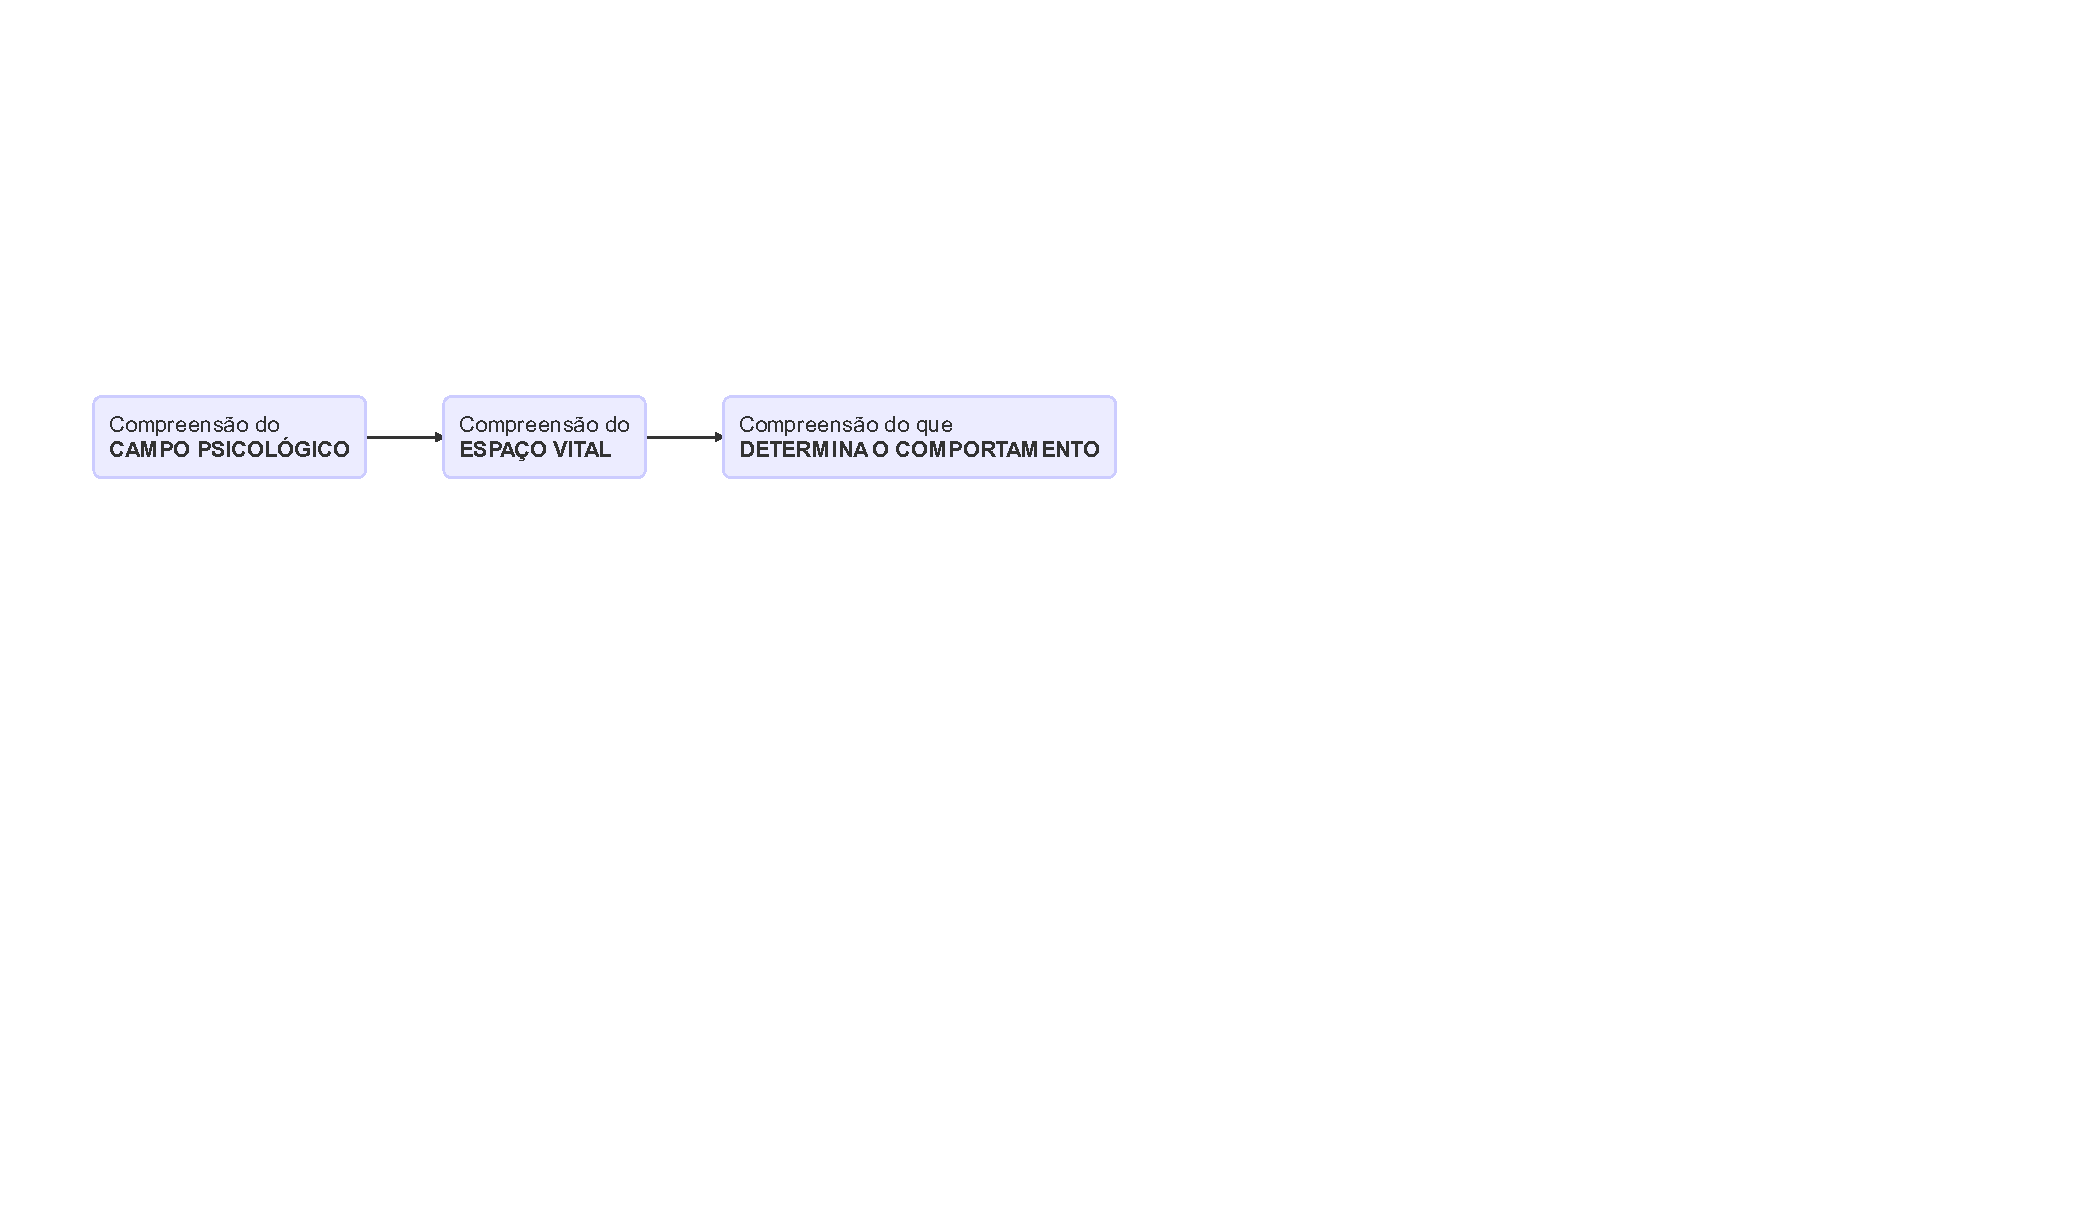
\includegraphics[width=1\linewidth]{Bookdown-Introducao-a-Psicologia_files/figure-latex/Compreensao do Campo Psicologico-1}

\hypertarget{a-compreensuxe3o-do-conceito-de-grupo-1}{%
\subsection{A Compreensão do CONCEITO DE GRUPO}\label{a-compreensuxe3o-do-conceito-de-grupo-1}}

\begin{itemize}
\tightlist
\item
  Praticamente todos os momentos de nossas vidas OCORREM dentro de GRUPOS;
\item
  Para Lewin:

  \begin{itemize}
  \tightlist
  \item
    A \textbf{CARACTERÍSTICA} ESSENCIALMENTE DEFINIDORA DE \textbf{GRUPO } é a \textbf{INTERDEPENDÊNCIA} de seus membros.
  \item
    Um grupo não é a \textbf{SOMA DE CARACTERÍSTICAS} de seus membros;
  \item
    Um grupo é \textbf{ALGO NOVO}, resultante dos \textbf{PROCESSOS QUE OCORREM} DENTRO DO GRUPO
  \item
    A MUNDANÇA DE UM MEMBRO PODE ALTERAR COMPLETAMENTE A DINÂMICA DO GRUPO;
  \end{itemize}
\item
  Os estudos de Lewin:

  \begin{itemize}
  \tightlist
  \item
    Deram ÊNFASE aos \textbf{PEQUENOS GRUPOS};
  \item
    Sobre os GRANDES GRUPOS: Ele considerava que a Psicologia não tinha INSTRUMENTAL SUCICIENTE para entender o estudo das GRANDES MASSAS;
  \end{itemize}
\end{itemize}

\hypertarget{o-conceito-de-campo-psicoluxf3gico-e-a-psicologia-social-1}{%
\subsection{O conceito de CAMPO PSICOLÓGICO e a PSICOLOGIA SOCIAL}\label{o-conceito-de-campo-psicoluxf3gico-e-a-psicologia-social-1}}

\begin{itemize}
\tightlist
\item
  Lewin criou o conceito de CAMPO SOCIAL que é formado pelo GRUPO e pelo AMBIENTE;
\item
  Umas das CARACTERÍSTICAS DO GRUPO é o CLIMA SOCIAL;
\item
  Existe uma LIDERANÇA NO GRUPO

  \begin{itemize}
  \tightlist
  \item
    Tipos de LIDERANÇA:

    \begin{itemize}
    \tightlist
    \item
      Autocrática
    \item
      Democrática
    \item
      \emph{Leissez-faire}
    \end{itemize}
  \end{itemize}
\item
  Lewin pesquisou a DINÂMICA GRUPAL atrvés de um TRABALHO EXPERIMENTAL minucioso;
\item
  As contribuições de Kurt Lewin:

  \begin{itemize}
  \tightlist
  \item
    Estão presentes até hoje;
  \item
    Embasam:

    \begin{itemize}
    \tightlist
    \item
      OUTRAS TEORIAS que envolvem grupos;
    \item
      TÉCNICAS de trabalho com grupos
    \end{itemize}
  \end{itemize}
\end{itemize}

\hypertarget{resumo-do-capuxedtulo-5---a-psicanuxe1lise-1}{%
\section{Resumo do Capítulo 5 - A Psicanálise}\label{resumo-do-capuxedtulo-5---a-psicanuxe1lise-1}}

\begin{itemize}
\tightlist
\item
  Em breve, disponibilizaremos.
\end{itemize}

\hypertarget{resumo-do-capuxedtulo-7---a-psicologia-do-desenvolvimento-1}{%
\section{Resumo do Capítulo 7 - A Psicologia do Desenvolvimento}\label{resumo-do-capuxedtulo-7---a-psicologia-do-desenvolvimento-1}}

\begin{itemize}
\tightlist
\item
  Em breve, disponibilizaremos.
\end{itemize}

\hypertarget{livro-teorias-da-personalidade-feist-feist-roberts-2014-1}{%
\section{\texorpdfstring{Livro: \textbf{Teorias da Personalidade} (FEIST; FEIST; ROBERTS, 2014)}{Livro: Teorias da Personalidade (FEIST; FEIST; ROBERTS, 2014)}}\label{livro-teorias-da-personalidade-feist-feist-roberts-2014-1}}

\begin{figure}

{\centering 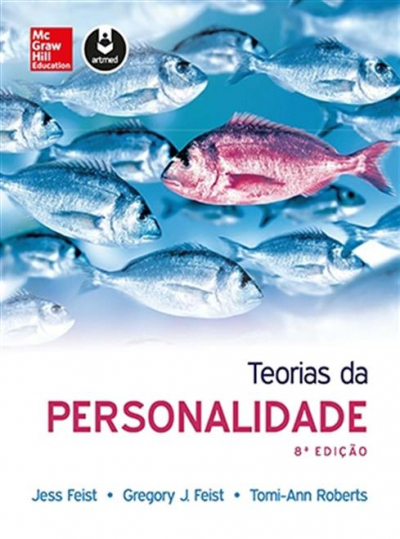
\includegraphics[width=0.8\linewidth]{figuras/Livro-Teorias-da-Personalidade} 

}

\caption{Livro Teorias da Personalidade}\label{fig:unnamed-chunk-22}
\end{figure}

\hypertarget{resumo-do-capuxedtulo-9---maslow-teoria-holuxedstico-dinuxe2mica-1}{%
\section{Resumo do Capítulo 9 - Maslow: Teoria-Holístico-Dinâmica}\label{resumo-do-capuxedtulo-9---maslow-teoria-holuxedstico-dinuxe2mica-1}}

\begin{itemize}
\tightlist
\item
  Em breve, disponibilizaremos.
\end{itemize}

\hypertarget{resumo-do-capuxedtulo-10---rogers-teoria-centrada-na-pessoa-1}{%
\section{Resumo do Capítulo 10 - Rogers: Teoria Centrada na Pessoa}\label{resumo-do-capuxedtulo-10---rogers-teoria-centrada-na-pessoa-1}}

\begin{itemize}
\tightlist
\item
  Em breve, disponibilizaremos.
\end{itemize}

\hypertarget{livro-introduuxe7uxe3o-uxe0-psicologia-feldman-2015-1}{%
\section{\texorpdfstring{Livro: \textbf{Introdução à Psicologia} (FELDMAN, 2015)\protect\hyperlink{feldman}{*}}{Livro: Introdução à Psicologia (FELDMAN, 2015)*}}\label{livro-introduuxe7uxe3o-uxe0-psicologia-feldman-2015-1}}

Figura Livro - FELDMAN, Robert S. \textbf{Introdução à Psicologia}. 10.ed. Porto Alegre: AMGH Editora, 2015

\hypertarget{capuxedtulo-1---muxf3dulo-3---livro-introduuxe7uxe3o-uxe0-psicologia-1}{%
\subsection{Capítulo 1 - Módulo 3 - Livro Introdução à Psicologia}\label{capuxedtulo-1---muxf3dulo-3---livro-introduuxe7uxe3o-uxe0-psicologia-1}}

Capítulo 1 - Módulo 3 - Livro Introdução à Psicologia1

\begin{itemize}
\tightlist
\item
  Na pesquisa de arquivo, dados existentes são usados para testar uma hipótese, tais como:

  \begin{itemize}
  \tightlist
  \item
    Documentos censitários;
  \item
    Registros universitários;
  \item
    Recortes de jornal; etc.
  \end{itemize}
\item
  \textbf{Vantagens}:

  \begin{itemize}
  \tightlist
  \item
    É um meio econômico de testar hipóteses que alguém já coletou os dados básicos.
  \end{itemize}
\item
  \textbf{Desvantagens} do uso de dados já existentes:

  \begin{itemize}
  \tightlist
  \item
    Os dados podem não estar dispostos em uma forma que permita o pesquisador testar uma hipótese plenamente.
  \item
    As informações podem estar incompletas;
  \item
    As informações podem ter sido coletadas arbitrariamente;
  \item
    O que é mais comum: Os registros com as informações necessárias muitas vezes não existem;

    \begin{itemize}
    \tightlist
    \item
      Nesse caso, pode-se recorrer a outro método de pesquisa: \textbf{Observação naturalista}.
    \end{itemize}
  \end{itemize}
\end{itemize}

Capítulo 1 - Módulo 3 - Livro Introdução à Psicologia1

\begin{itemize}
\tightlist
\item
  O observador examina \textbf{um comportamento que ocorre naturalmente} e que \textbf{ele não interfere na situação};

  \begin{itemize}
  \tightlist
  \item
    O pesquisados simplesmente registra o que acontece
  \item
    O pesquisador não faz modificações na situação que está sendo observada;

    \begin{itemize}
    \tightlist
    \item
      Exemplo:

      \begin{itemize}
      \tightlist
      \item
        O pesquisador observa e registra o \textbf{tipo de ajuda prestada} em uma área urbana com alto índice de criminalidade.
      \end{itemize}
    \end{itemize}
  \item
    Vantagem: Obtemos uma amostra do que as pessoas fazem em seu \emph{habitat};
  \item
    INCONVENIENTES:

    \begin{itemize}
    \tightlist
    \item
      A \textbf{impossibilidade de controlar} qualquer um dos \textbf{fatores de interesse};
    \item
      Poucos casos cuja previsibilidade permita observar dificultando a formulação de conclusões;
    \item
      É preciso esperar que as condições apropriadas (\textbf{fatores de interesse}) ocorram;
    \item
      Caso os participantes saibam ou percebam que estão sendo vigiados eles podem:

      \begin{itemize}
      \tightlist
      \item
        Alterar as suas reações;
      \item
        Produzir um comportamento que não é verdadeiramente representativo
      \end{itemize}
    \end{itemize}
  \end{itemize}
\end{itemize}

\begin{quote}
\begin{quote}
\begin{quote}
\begin{quote}
\begin{quote}
\begin{quote}
ACRESCENTAR LINK PARA SECAO DO RESUMO DOS LIVROS
\end{quote}
\end{quote}
\end{quote}
\end{quote}
\end{quote}
\end{quote}

Capítulo 1 - Módulo 3 - Livro Introdução à Psicologia1

\begin{itemize}
\tightlist
\item
  É um método simples e direto de conhecer, através de uma pergunta direta, o que as pessoas:

  \begin{itemize}
  \tightlist
  \item
    Pensam
  \item
    Sentem
  \item
    Fazem
  \end{itemize}
\item
  Através desse método, uma \textbf{amostra} de pessoas é escolhida para representar um \textbf{grupo de interesse} mais amplo. (\textbf{Uma população}), buscando-se conhecer:

  \begin{itemize}
  \tightlist
  \item
    Sobre seu \textbf{comportamento};
  \item
    Sobre seus \textbf{pensamentos};
  \item
    Sobre suas \textbf{Atitudes};
  \end{itemize}
\item
  Os pesquisadores conseguem deduzir com notável precisão como um grande grupo responderia;

  \begin{itemize}
  \tightlist
  \item
    Exemplos:

    \begin{itemize}
    \tightlist
    \item
      Pesquisadores que realizam \textbf{investigação sobre comportamento de ajuda}

      \begin{itemize}
      \tightlist
      \item
        Podem realizar uma pesquisa pedindo às pessoas que completem um \textbf{questionário} no qual elas indicam \textbf{sua relutância em prestar auxílio a alguém};
      \end{itemize}
    \item
      Pesquisadores interessados em \textbf{aprender sobre práticas sexuais}
    \item
      Podem realizar \textbf{levantamento} para \textbf{verificar quais práticas sexuais} \textbf{comuns} e quais \textbf{não são comuns}.
    \item
      Finalidade: Mapear as mudanças de noções de moralidade sexual durante as últimas décadas.
    \end{itemize}
  \end{itemize}
\item
  Desvantagens e armadilhas

  \begin{itemize}
  \tightlist
  \item
    É trabalhosa a \textbf{constituição de uma amostra estatísticamente representativa} (\textbf{amostra aleatória}) em que cada participante tenha a mesma chance (probabilidade) de ser incluído na amostra;
  \item
    Se a amostra não for \textbf{estatísticamente representativa} da população de interesse, os resultados da pesquisa terão pouco significado;
  \item
    Entrevistados podem não querer admitir:

    \begin{itemize}
    \tightlist
    \item
      Que tem comportamentos e/ou atitudes \textbf{socialmente indesejáveis};
    \item
      Que tem comportamento e/ou atitudes considerados por outras pessoas como \textbf{anormais};
    \item
      O que fazem em sua \textbf{intimidade};
    \end{itemize}
  \item
    Entrevistados podem \textbf{nem ter a consciência de quais são suas verdadeiras atitudes} ou porque elas as mantêm.
  \end{itemize}
\end{itemize}

Capítulo 1 - Módulo 3 - Livro Introdução à Psicologia1

\begin{itemize}
\tightlist
\item
  É uma investigação intensiva e em profundidade de \textbf{um único indivíduo} ou de \textbf{um pequeno grupo}.
\item
  Muitas vezes incluem \textbf{testagem psicológica}

  \begin{itemize}
  \tightlist
  \item
    É um procedimento em que um conjunto cuidadosamente elaborado de \textbf{instrumentos} é usado para \textbf{compreender algum }aspecto da personalidade** daquele indivíduo ou grupo**.
  \end{itemize}
\item
  Objetivos da realização de estudos de caso:

  \begin{itemize}
  \tightlist
  \item
    Aprender sobre os poucos indivíduos que estão sendo examinados;
  \item
    Usar conhecimentos adquiridos (a partir do estudo) para aperfeiçoar nossa compreensão das pessoas em geral.
  \end{itemize}
\item
  Comentários e curiosidades:
  * Sigmund Freud desenvolveu suas teorias por meio de \textbf{estudos de caso} de alguns de seus pacientes;
  * Estudos de casos de terroristas podem \textbf{ajudar a identificar indivíduos que são propensos à violência};
\item
  Desvantagens e inconvenientes:

  \begin{itemize}
  \tightlist
  \item
    Se os indivíduos examinados são excepcionais em algum aspecto, não é apropriado fazer generalizações para uma população mais ampla.
    \textgreater{} Observação: Mesmo em sua excepcionalidade, indivíduos ou pequenos grupos de indivíduos podem abrir caminho para \textbf{teorias} e \textbf{tratamentos} novos para \textbf{transtornos psicológicos}.
  \end{itemize}
\end{itemize}

Capítulo 1 - Módulo 3 - Livro Introdução à Psicologia1

De acordo com Feldman(2015, p.~31), os pesquisadores muitas vezes desejam determinar a relação entre duas variáveis.

\begin{itemize}
\tightlist
\item
  Variáveis são \textbf{comportamentos}, \textbf{eventos} ou \textbf{outras características} que podem mudar ou variar de alguma maneira.

  \begin{itemize}
  \tightlist
  \item
    Exemplo: Uma pesquisa para verificar se a quantidade de estudo faz diferença nas notas em provas, as
    variáveis seriam \textbf{tempo de estudo} e \textbf{escores} em provas.
  \end{itemize}
\end{itemize}

Na pesquisa correlacional, dois conjuntos de variáveis são examinados para determinar se eles estão associados ou ``correlacionados''.

\begin{itemize}
\tightlist
\item
  A \textbf{força} e a \textbf{direção} da relação entre as duas variáveis são representadas por uma estatística matemática conhecida como correlação (ou, mais formalmente, como coeficiente de correlação), que pode variar de +1,0 a -1,0.
\item
  Uma \textbf{correlação positiva} indica que, à medida que uma variável aumenta, podemos prever que o valor da outra variável também aumentará.

  \begin{itemize}
  \tightlist
  \item
    Por exemplo, se previrmos que, quanto mais tempo os alunos passam estudando para uma prova, maiores serão suas notas e que, quanto menos eles estudam, menor serão suas pontuações nas provas, estamos esperando encontrar uma correlação positiva. (Valores mais altos da variável ``quantidade de tempo de estudo'' estariam associados a valores mais altos da variável ``pontuação na prova'', enquanto menores valores da ``quantidade de tempo de estudo'' estariam associados a valores mais baixos da variável ``pontuação na prova''.)
  \item
    A correlação, então, seria indicada por um número positivo e, quanto mais forte for a associação entre estudar e pontuação nas provas, mais próximo de 1,0 será o número.
  \end{itemize}
\item
  Em contraste, uma \textbf{correlação negativa} demonstra que, à medida que o valor de uma variável aumenta, o valor de outra diminui. Por exemplo, podemos prever que, à medida que o número de horas passadas estudando aumenta, o número de horas passadas participando de festas diminui. Nesse caso, estamos esperando uma correlação negativa, que varia entre 0 e -1,0.

  \begin{itemize}
  \tightlist
  \item
    Mais estudo está associado a menor participação em festas, enquanto menos estudo está associado a maior participação em festas. Quanto mais forte for a associação entre estudar e participar de festas, mais próxima será a correlação de -1,0. Por exemplo, uma correlação de -0,85 indicaria uma associação negativa forte entre participar de festas e estudar.
  \end{itemize}
\item
  Evidentemente, é bem possível que exista \textbf{pouca ou nenhuma relação} entre duas variáveis.

  \begin{itemize}
  \tightlist
  \item
    Por exemplo, provavelmente \textbf{não esperaríamos encontrar uma relação} entre o \textbf{número de horas de estudo} e \textbf{altura}. A ausência de uma relação seria indicada por uma correlação próxima de 0. Por exemplo, se encontrássemos uma correlação de -0,02 ou 0,03, isso indicaria que existe praticamente nenhuma associação entre duas variáveis: saber o quanto alguém estuda nos diz nada sobre sua altura.
  \end{itemize}
\item
  Quando duas variáveis estão fortemente correlacionadas, somos tentados a presumir que uma variável causa a outra. Por exemplo, se descobrirmos que mais estudo está associado a notas mais altas, podemos supor que estudar mais causa notas mais altas. Embora esta não seja uma má suposição, ela continua sendo apenas uma suposição -- porque descobrir que suas variáveis estão correlacionadas não significa que exista uma relação causal entre elas.

  \begin{itemize}
  \tightlist
  \item
    A \textbf{correlação forte} sugere que saber o quanto uma pessoa estuda pode ajudar-nos a prever como aquela
    pessoa vai se sair em uma prova, mas isso não significa que estudar causa o desempenho na prova.

    \begin{itemize}
    \tightlist
    \item
      Em vez disso, por exemplo, as \textbf{pessoas que estão mais interessadas no assunto} poderiam estudar mais do que aquelas que estão menos interessadas; assim, a \textbf{quantidade de interesse}, e não o número de horas passadas estudando, preveria o desempenho em provas.
    \end{itemize}
  \item
    O simples fato de que \textbf{duas variáveis ocorrem juntas} \textbf{não significa que uma cause a outra}. Simplesmente fornecem uma medida da força da relação entre duas variáveis

    \begin{itemize}
    \tightlist
    \item
      Exemplos:

      \begin{itemize}
      \tightlist
      \item
        Suponha que você descobriu que o \textbf{número de lugares de prática religiosa} em uma grande amostra de cidades estava positivamente relacionado ao \textbf{número de pessoas detidas}, significando que, quanto mais lugares de prática religiosa, mais detenções havia em uma cidade. Isso significa que a presença de mais espaços de prática religiosa causou o maior número de detenções? Quase certamente não, é claro. \textbf{Nesse caso, a causa subjacente é o tamanho da cidade}: em cidades maiores, existem mais espaços de prática religiosa tanto como de mais detenções.
      \item
        Crianças que assistem a muitos programas de televisão com alto nível de agressão são propensas a demonstrar um grau relativamente alto de comportamento agressivo e que aquelas que assistem menos a programas de televisão que retratam agressão são inclinadas a exibir um grau relativamente baixo desse comportamento (ver Fig. 2). Contudo, \textbf{não podemos dizer que a agressão é causada por ver televisão}, pois \textbf{muitas outras explicações são possíveis}. Pessoas que já são altamente agressivas poderiam escolher ver programas com um alto conteúdo agressivo porque elas são agressivas
      \end{itemize}
    \end{itemize}
  \end{itemize}
\item
  Desvantagem da pesquisa correlacional:

  \begin{itemize}
  \tightlist
  \item
    A \textbf{impossibilidade} de a pesquisa correlacional \textbf{demonstrar relações de causa e efeito} é uma desvantagem crucial para seu uso. Contudo, existe uma técnica alternativa que estabelece causalidade: \textbf{o experimento}.
  \end{itemize}
\item
  EXPERIMENTO: Investigação da relação entre duas (ou mais) variáveis alterando--se deliberadamente uma situação e observando-se os efeitos dessa alteração em outros aspectos da situação.
\end{itemize}

\hypertarget{muxe9todo-cientuxedfico-muxe9todo-experimental-1}{%
\subsection{Método Científico: Método Experimental}\label{muxe9todo-cientuxedfico-muxe9todo-experimental-1}}

\hypertarget{pesquisa-experimental-1}{%
\subsection{Pesquisa Experimental}\label{pesquisa-experimental-1}}

Slides

\begin{itemize}
\tightlist
\item
  Os estudo experimental é o método para estabelecer explicações, de demonstrar a relação de causa e efeito.
\item
  \textbf{HIPÓTESE}: É uma afirmação. Os experimentos iniciam se com uma hipótese , acerca dos eventos, conhecidos como variáveis.
\item
  A essência de um Experimento:

  \begin{itemize}
  \tightlist
  \item
    Os pesquisadores deliberadamente manipulam a variável independente o evento cuja influência está sendo investigada
  \item
    Eles pedem que variáveis estranhas ou irrelevantes afetem os resultados do estudo
  \item
    Eles medem os efeitos da manipulação sobre a variável dependente
  \end{itemize}
\item
  Exemplo:

  \begin{itemize}
  \tightlist
  \item
    \textbf{Objetivo}: Será que o perfume desencadeia vivências nostálgicas e aumenta afetos positivos, autoestima e conexão social?
  \item
    \textbf{Hipótese}: Os participantes na condição experimental apresentará níveis mais elevados de afetos positivos, autoestima e apoio social
  \item
    \textbf{Método}: Participaram 160 pessoas. Metade para a condição experimental (12 perfumes) e outra metade condição controle (sem exposição do perfume)
  \item
    \textbf{Resultados}: Os participantes na condição experimental, apresentou mais
    afetos positivos, autoestima e apoio social, comparado ao grupo controle
  \end{itemize}
\end{itemize}

Capítulo 1 - Módulo 3 - Livro Introdução à Psicologia1

\begin{itemize}
\tightlist
\item
  Em um experimento formal, o pesquisador investiga a relação entre duas (ou mais) variáveis \textbf{alterando deliberadamente uma variável} em uma \textbf{situação controlada} e \textbf{observando os efeitos daquela mudança} em \textbf{outros aspectos da situação}.
\item
  Em um experimento, portanto, as condições são \textbf{criadas} e \textbf{controladas} pelo pesquisador, que deliberadamente faz uma alteração nessas condições a fim de observar os efeitos daquela mudança.
\item
  A alteração que o pesquisador deliberadamente faz em um experimento é denominada manipulação experimental. Manipulações experimentais são usadas para detectar relações entre diferentes variáveis (Staub, 2011 apud Feldman, 2015).
\item
  A realização de um experimento envolve \textbf{várias etapas}, mas o processo geralmente se \textbf{inicia} com o \textbf{desenvolvimento de uma ou mais hipóteses} a serem testadas pelo experimento.

  \begin{itemize}
  \tightlist
  \item
    Por exemplo, \textbf{Latané} e \textbf{Darley}, ao testar sua \textbf{teoria} acerca da \textbf{difusão da responsabilidade no comportamento de espectadores}, elaboraram a seguinte hipótese: quanto maior for o número de pessoas que testemunham uma situação de emergência, menor será a probabilidade de que alguma delas ajude a vítima.
  \item
    Eles então criaram um experimento para testar essa hipótese.

    \begin{itemize}
    \tightlist
    \item
      O \textbf{primeiro passo} foi formular uma definição operacional da hipótese, conceitualizando-a de um modo que ela pudesse ser testada.
    \item
      Latané e Darley tiveram de levar em conta o princípio fundamental da pesquisa experimental mencionado anteriormente: os experimentadores \textbf{devem manipular ao menos uma variável a fim de observar os efeitos da manipulação em outra variável}, enquanto outros fatores na situação são mantidos constantes.
    \item
      Entretanto, a manipulação não pode ser vista isoladamente; para que uma relação de causa e efeito seja estabelecida, os efeitos da manipulação devem ser comparados com os efeitos de nenhuma manipulação ou de outro tipo de manipulação.
    \end{itemize}
  \end{itemize}
\end{itemize}

\hypertarget{grupos-experimentais-e-grupos-controle-1}{%
\subsection{Grupos experimentais e grupos-controle}\label{grupos-experimentais-e-grupos-controle-1}}

\begin{itemize}
\tightlist
\item
  A pesquisa experimental exige, portanto, que as respostas de ao menos dois grupos sejam comparadas.
\item
  Um grupo receberá um tratamento especial -- a manipulação implementada pelo experimentador -- e outro grupo receberá um tratamento diferente ou nenhum tratamento.
\item
  Qualquer grupo que recebe um tratamento é denominado grupo experimental
\item
  Um grupo que não recebe tratamento é denominado grupo-controle
\item
  Em alguns experimentos, existem vários grupos experimentais e de controle, cada um dos quais comparado com outro grupo.
\item
  \textbf{Empregando} \textbf{grupos experimentais} e de \textbf{controle} em um experimento, os pesquisadores são capazes de descartar a \textbf{possibilidade de que alguma outra variável que não a manipulação experimental tenha produzido os resultados observados no experimento}.
\item
  Sem um grupo-controle, não poderíamos ter certeza de que alguma outra variável, como, por exemplo, a temperatura no momento da execução do experimento, a cor de cabelo do experimentador ou mesmo a mera passagem do tempo, não estava causando as mudanças observadas.

  \begin{itemize}
  \tightlist
  \item
    Por exemplo:

    \begin{itemize}
    \tightlist
    \item
      Considere um pesquisador de medicina que acredita que inventou um medicamento que cura o resfriado.
    \item
      Para testar sua alegação, ele administra o remédio um dia a um grupo de 20 pessoas que estão resfriadas e descobre que 10 dias depois todas elas estão curadas.
    \item
      Eureca? Mais devagar. Um observador que considere esse estudo falho poderia argumentar sensatamente que as pessoas teriam melhorado mesmo sem o medicamento.
    \item
      O que o pesquisador evidentemente precisava era de um grupo-controle formado por pessoas resfriadas que não recebem o remédio e cuja saúde também é verificada 10 dias depois.
    \end{itemize}
  \end{itemize}
\item
  Somente quando existe uma diferença significativa entre grupos experimental e de controle é que a eficácia do remédio pode ser avaliada. Ao usar grupos-controle, então, os pesquisadores podem isolar causas específicas para seus achados -- e extrair inferências de causa e efeito.
\item
  Voltando ao experimento de Latané e Darley:

  \begin{itemize}
  \tightlist
  \item
    Vemos que os pesquisadores recisavam traduzir sua hipótese para algo que pudesse ser testado.
  \item
    Para fazer isso, decidiram criar uma falsa situação de emergência que pareceria requerer a ajuda de um espectador.
  \item
    Como manipulação experimental, optaram por \textbf{variar o número de espectadores presentes}.
  \item
    Eles poderiam ter usado apenas \textbf{um grupo experimental}, por exemplo, de duas pessoas presentes, e \textbf{um grupo-controle} com apenas uma pessoa presente para fins de comparação.
  \item
    Em vez disso, optaram por um procedimento mais complexo envolvendo a \textbf{criação de grupos de três tamanhos} -- compostos por \textbf{duas}, \textbf{três} e \textbf{seis} pessoas -- que poderiam ser comparados um com o outro.
  \end{itemize}
\end{itemize}

\hypertarget{variuxe1veis-independentes-e-dependentes-1}{%
\subsection{Variáveis Independentes e Dependentes}\label{variuxe1veis-independentes-e-dependentes-1}}

\begin{itemize}
\tightlist
\item
  O projeto experimental de Latané e Darley agora incluía uma definição experimental do que é chamado de variável independente.
\item
  A variável independente é a condição que é manipulada por um experimentador.

  \begin{itemize}
  \tightlist
  \item
    Você pode pensar a variável independente como sendo independente das ações daqueles que participam de um experimento; ela é controlada pelo experimentador.
  \item
    No caso do experimento de Latané e Darley, a variável independente era o número de pessoas presentes, que foi manipulado pelos experimentadores.
  \end{itemize}
\item
  O próximo passo era decidir como eles determinariam o efeito que o número variável de espectadores tinha no comportamento das pessoas no experimento.
\item
  Fundamental em todo experimento é a VARIÁVEL DEPENDENTE, aquela que é medida e que se espera que mude em função das alterações provocadas pelo experimentador manipulando a \textbf{variável independente}.
\item
  A variável dependente é dependente das ações dos participantes ou sujeitos -- as pessoas que participam de um experimento.

  \begin{itemize}
  \tightlist
  \item
    Latané e Darley tinham várias escolhas possíveis para sua medida dependente.
  \item
    Uma poderia ter sido uma simples verificação (sim/não) do comportamento de ajuda dos participantes.
  \item
    Contudo, os investigadores também queriam uma análise mais precisa do comportamento de ajuda.
  \item
    Consequentemente, também mediram a quantidade de tempo que levava para um participante prestar ajuda. Latané e Darley agora tinham todos os componentes necessários de um experimento.
  \end{itemize}
\item
  A variável independente, manipulada por eles, era o \textbf{número de espectadores presentes} em uma situação de emergência.
\item
  A variável dependente era verificar se \textbf{os espectadores em cada um dos grupos prestavam ajuda} e a \textbf{quantidade de tempo} que eles levavam para isso.
\item
  Consequentemente, como todos os experimentos, esse teve tanto uma variável independente
  como uma variável dependente.
\item
  \textbf{Todos os verdadeiros experimentos em psicologia} \textbf{encaixam-se nesse modelo simples}.
\end{itemize}

\begin{quote}
TERMOS IMPORTANTES:
\textgreater{} \textbf{Variável Independente}: Variável que \textbf{é manipulada} por um experimentador.
\textgreater{} \textbf{Variável Dependente}: Variável que \textbf{é mensurada }e que \textbf{se espera que se modifique} como resultado de mudanças causadas pela manipulação da variável independente realizada pelo experimentador.
\end{quote}

\hypertarget{distribuiuxe7uxe3o-aleatuxf3ria-dos-participantes-1}{%
\subsection{Distribuição aleatória dos participantes}\label{distribuiuxe7uxe3o-aleatuxf3ria-dos-participantes-1}}

\begin{itemize}
\tightlist
\item
  Para tornar o experimento um teste válido da hipótese, Latané e Darley precisavam adicionar um passo final ao projeto experimental: designar corretamente os participantes a determinado grupo experimental.
\item
  O significado desse passo torna-se claro quando examinamos vários procedimentos alternativos. Por exemplo, os experimentadores poderiam ter designado somente homens para o grupo com dois espectadores, apenas mulheres para o grupo com três espectadores e ambos (homens e mulheres) para o grupo com seis espectadores. Contudo, caso tivessem feito isso, as eventuais diferenças que encontraram no comportamento de ajuda não poderiam ser atribuídas com certeza unicamente ao tamanho do grupo, pois elas poderiam igualmente ter resultado da composição do grupo. Um procedimento mais sensato seria assegurar que cada grupo tivesse a mesma composição em termos de gênero; assim, os pesquisadores teriam podido fazer comparações entre os grupos com mais precisão.
\item
  Os participantes em cada um dos grupos experimentais devem ser comparáveis, e é muito fácil criar grupos que sejam semelhantes em termos de gênero. No entanto, o problema torna-se um pouco mais traiçoeiro quando consideramos outras características dos participantes. Como podemos garantir que os participantes em cada grupo experimental serão igualmente inteligentes, extrovertidos, cooperativos, e assim por diante, quando a lista de características -- qualquer uma poderia ser importante -- é potencialmente infinita?
\item
  A solução é um procedimento simples, mas elegante, chamado de designação aleatória à condição.
\item
  Os participantes são designados para diferentes grupos experimentais, ou ``condições'', com base no acaso e somente no acaso. O experimentador poderia, por exemplo, fazer um sorteio com moeda para cada participante e designar um participante para um grupo quando desse ``cara'' e para outro grupo quando desse ``coroa''. A vantagem dessa técnica é que existe uma chance idêntica de que as características dos participantes se distribuirão entre os diversos grupos. Quando um pesquisador emprega distribuição aleatória -- o que na prática geralmente é realizado usando números aleatórios gerados por computador --, é provável que cada um dos grupos terá aproximadamente a mesma proporção de pessoas inteligentes, cooperativas, extrovertidas, do sexo masculino e feminino, e assim por diante.
\end{itemize}

Figura - Efeitos da substância \textbf{propanolol} (figura 3)

\begin{itemize}
\tightlist
\item
  A \textbf{Figura 3} do livro de FELDMAN apresenta outro exemplo de um experimento. Como todos os experimentos, esse inclui um conjunto de elementos-chave, que você deve lembrar ao considerar se um estudo científico é realmente um experimento.

  \begin{itemize}
  \tightlist
  \item
    Uma variável independente, a variável que é manipulada pelo experimentador.
  \item
    Uma variável dependente, a variável que é medida pelo experimentador e que se espera que mude como resultado da manipulação da variável independente.
  \item
    Um procedimento que distribui aleatoriamente os participantes em diferentes grupos experimentais, ou ``condições'', da variável dependente.
  \item
    Uma hipótese que prevê o efeito que a variável independente terá na variável dependente. Somente se todos esses elementos estiverem presentes é que um estudo científico pode ser considerado um experimento verdadeiro em que relações de causa e efeito podem ser determinadas. (Para um resumo dos diferentes tipos de pesquisa que discutimos, ver \textbf{Fig. 4} do livro de FELDMAN .)
  \end{itemize}
\end{itemize}

Figura - Estratégias de pesquisa (figura 4)

\hypertarget{outros-tuxf3picos-nuxe3o-abordados-1}{%
\subsection{Outros tópicos não abordados}\label{outros-tuxf3picos-nuxe3o-abordados-1}}

No capítulo 3 do livro de FELDMAN, ainda constam dois tópicos que não abordei aqui por terem baixa chance de serem explorados na prova o que não prejudica a compreenção da \textbf{Pesquisa Experimental}

\begin{itemize}
\tightlist
\item
  Latané e Darley estavam certos?
\item
  Indo além do estudo
\end{itemize}

\hypertarget{livro-introduuxe7uxe3o-uxe0-psicologia-davidoff-2001-1}{%
\section{\texorpdfstring{Livro: \textbf{Introdução à Psicologia} (DAVIDOFF, 2001)}{Livro: Introdução à Psicologia (DAVIDOFF, 2001)}}\label{livro-introduuxe7uxe3o-uxe0-psicologia-davidoff-2001-1}}

Figura - Livro Introdução à Psicologia (DAVIDOFF, 2001)

\hypertarget{capuxedtulo-xx-1}{%
\subsection{Capítulo XX}\label{capuxedtulo-xx-1}}

\begin{itemize}
\tightlist
\item
  A definir.
\end{itemize}

Referências Bibliográficas

BOCH, Ana Mercês Bahia; FURTADO, Odair; TEIXEIRA, Maria de Lourdes Trassi. Psicologias: Uma Introdução ao Estudo da Psicologia. 13.ed. São Paulo: Saraiva, 2001.

DAVIDOFF, Linda L. \textbf{Introdução à Psicologia}. 3.ed. São Paulo:Pearson, 2001

FEIST, Jess; FEIST, Gregory J.; ROBERTS, Tomi-Ann. \textbf{Teorias da Personalidade}. 8.ed. Porto Alegre:AMGH, 2014

FELDMAN, Robert S. \textbf{Introdução à Psicologia}. 10.ed. Porto Alegre: AMGH Editora, 2015

KURT LEWIN. In: WIKIPÉDIA: a enciclopédia livre. Wikimedia, 2022. Disponível em: \textless{}\url{https://en.wikipedia.org/wiki/Kurt_Lewin}\textgreater. Acesso em: 30 set. 2022.

\hypertarget{notas-de-aula-1}{%
\chapter{Notas de Aula}\label{notas-de-aula-1}}

Neste capítulo estarão contidas todas as minhas notas de aula da disciplina.

\hypertarget{nota-de-aula-01---assuntos-da-aula-1}{%
\section{Nota de Aula 01 - ASSUNTOS DA AULA}\label{nota-de-aula-01---assuntos-da-aula-1}}

\begin{longtable}[]{@{}ll@{}}
\toprule()
Data & Tópicos Abordados \\
\midrule()
\endhead
dd/mm/aaaa & - Tópico 1- Tópico 2- Tópico 3 \\
\bottomrule()
\end{longtable}

\hypertarget{seuxe7uxe3o-numerada-1-15}{%
\subsection{Seção Numerada 1}\label{seuxe7uxe3o-numerada-1-15}}

Para \citet{BOCK2001}, tornamo-nos pouco compreensíveis se não recorrermos a \ldots.

\hypertarget{seuxe7uxe3o-nuxe3o-numerada-1-30}{%
\subsection*{Seção não Numerada 1}\label{seuxe7uxe3o-nuxe3o-numerada-1-30}}
\addcontentsline{toc}{subsection}{Seção não Numerada 1}

Para \citet{BOCK2001}, tornamo-nos pouco compreensíveis se não recorrermos a \ldots.

\hypertarget{seuxe7uxe3o-nuxe3o-numerada-2-45}{%
\subsection*{Seção não Numerada 2}\label{seuxe7uxe3o-nuxe3o-numerada-2-45}}
\addcontentsline{toc}{subsection}{Seção não Numerada 2}

Para \citet{BOCK2001}, tornamo-nos pouco compreensíveis se não recorrermos a \ldots.

\hypertarget{seuxe7uxe3o-numerada-2-15}{%
\subsection{Seção Numerada 2}\label{seuxe7uxe3o-numerada-2-15}}

Para \citet{BOCK2001}, tornamo-nos pouco compreensíveis se não recorrermos a \ldots.

\hypertarget{seuxe7uxe3o-nuxe3o-numerada-1-31}{%
\subsection*{Seção não Numerada 1}\label{seuxe7uxe3o-nuxe3o-numerada-1-31}}
\addcontentsline{toc}{subsection}{Seção não Numerada 1}

Para \citet{BOCK2001}, tornamo-nos pouco compreensíveis se não recorrermos a \ldots.

Para \citet{DAVIDOFF2001}, deve-se lembrar que\ldots.

\hypertarget{seuxe7uxe3o-nuxe3o-numerada-2-46}{%
\subsection*{Seção não Numerada 2}\label{seuxe7uxe3o-nuxe3o-numerada-2-46}}
\addcontentsline{toc}{subsection}{Seção não Numerada 2}

Para \citet{BOCK2001}, tornamo-nos pouco compreensíveis se não recorrermos a \ldots.

Para \citet{DAVIDOFF2001}, deve-se lembrar que\ldots.

\hypertarget{seuxe7uxe3o-nuxe3o-numerada-2-47}{%
\subsection*{Seção não Numerada 2}\label{seuxe7uxe3o-nuxe3o-numerada-2-47}}
\addcontentsline{toc}{subsection}{Seção não Numerada 2}

Para \citet{BOCK2001}, tornamo-nos pouco compreensíveis se não recorrermos a \ldots.

Para \citet{DAVIDOFF2001}, deve-se lembrar que\ldots.

\hypertarget{notas-de-aula-02---assuntos-da-aula-1}{%
\section{Notas de Aula 02 - ASSUNTOS DA AULA}\label{notas-de-aula-02---assuntos-da-aula-1}}

\begin{longtable}[]{@{}ll@{}}
\toprule()
Data & Tópicos Abordados \\
\midrule()
\endhead
dd/mm/aaaa & - Tópico 1- Tópico 2- Tópico 3 \\
\bottomrule()
\end{longtable}

\hypertarget{seuxe7uxe3o-numerada-1-16}{%
\subsection{Seção Numerada 1}\label{seuxe7uxe3o-numerada-1-16}}

Para \citet{BOCK2001}, tornamo-nos pouco compreensíveis se não recorrermos a \ldots.

\hypertarget{seuxe7uxe3o-nuxe3o-numerada-1-32}{%
\subsection*{Seção não Numerada 1}\label{seuxe7uxe3o-nuxe3o-numerada-1-32}}
\addcontentsline{toc}{subsection}{Seção não Numerada 1}

Para \citet{BOCK2001}, tornamo-nos pouco compreensíveis se não recorrermos a \ldots.

\hypertarget{seuxe7uxe3o-nuxe3o-numerada-2-48}{%
\subsection*{Seção não Numerada 2}\label{seuxe7uxe3o-nuxe3o-numerada-2-48}}
\addcontentsline{toc}{subsection}{Seção não Numerada 2}

Para \citet{BOCK2001}, tornamo-nos pouco compreensíveis se não recorrermos a \ldots.

\hypertarget{seuxe7uxe3o-numerada-2-16}{%
\subsection{Seção Numerada 2}\label{seuxe7uxe3o-numerada-2-16}}

Para \citet{BOCK2001}, tornamo-nos pouco compreensíveis se não recorrermos a \ldots.

\hypertarget{seuxe7uxe3o-nuxe3o-numerada-1-33}{%
\subsection*{Seção não Numerada 1}\label{seuxe7uxe3o-nuxe3o-numerada-1-33}}
\addcontentsline{toc}{subsection}{Seção não Numerada 1}

Para \citet{BOCK2001}, tornamo-nos pouco compreensíveis se não recorrermos a \ldots.

Para \citet{DAVIDOFF2001}, deve-se lembrar que\ldots.

\hypertarget{seuxe7uxe3o-nuxe3o-numerada-2-49}{%
\subsection*{Seção não Numerada 2}\label{seuxe7uxe3o-nuxe3o-numerada-2-49}}
\addcontentsline{toc}{subsection}{Seção não Numerada 2}

Para \citet{BOCK2001}, tornamo-nos pouco compreensíveis se não recorrermos a \ldots.

Para \citet{DAVIDOFF2001}, deve-se lembrar que\ldots.

\hypertarget{seuxe7uxe3o-nuxe3o-numerada-2-50}{%
\subsection*{Seção não Numerada 2}\label{seuxe7uxe3o-nuxe3o-numerada-2-50}}
\addcontentsline{toc}{subsection}{Seção não Numerada 2}

Para \citet{BOCK2001}, tornamo-nos pouco compreensíveis se não recorrermos a \ldots.

Para \citet{DAVIDOFF2001}, deve-se lembrar que\ldots.

\hypertarget{nas-pruxf3ximas-aulas-6}{%
\section{Nas próximas aulas}\label{nas-pruxf3ximas-aulas-6}}

Veja, de acordo com o plano da disciplina, o que já foi estudado e o que ainda será ministrado nas próximas aulas:

Tópico 1
Tópico 2
Tórico 3

\hypertarget{notas-de-aula-de-outros-alunos-1}{%
\chapter{Notas de Aula de Outros Alunos}\label{notas-de-aula-de-outros-alunos-1}}

Neste capítulo estarão contidas todas as notas de aula da disciplina elaboradas por outros alunos que autorizaram a sua publicação e disponibilização.

\hypertarget{aula-01---assuntos-da-aula-4}{%
\section{Aula 01 - ASSUNTOS DA AULA}\label{aula-01---assuntos-da-aula-4}}

\begin{longtable}[]{@{}ll@{}}
\toprule()
Data & Tópicos Abordados \\
\midrule()
\endhead
dd/mm/aaaa & - Tópico 1- Tópico 2- Tópico 3 \\
\bottomrule()
\end{longtable}

\hypertarget{seuxe7uxe3o-numerada-1-17}{%
\subsection{Seção Numerada 1}\label{seuxe7uxe3o-numerada-1-17}}

Para \citet{BOCK2001}, tornamo-nos pouco compreensíveis se não recorrermos a \ldots.

\hypertarget{seuxe7uxe3o-nuxe3o-numerada-1-34}{%
\subsection*{Seção não Numerada 1}\label{seuxe7uxe3o-nuxe3o-numerada-1-34}}
\addcontentsline{toc}{subsection}{Seção não Numerada 1}

Para \citet{BOCK2001}, tornamo-nos pouco compreensíveis se não recorrermos a \ldots.

\hypertarget{seuxe7uxe3o-nuxe3o-numerada-2-51}{%
\subsection*{Seção não Numerada 2}\label{seuxe7uxe3o-nuxe3o-numerada-2-51}}
\addcontentsline{toc}{subsection}{Seção não Numerada 2}

Para \citet{BOCK2001}, tornamo-nos pouco compreensíveis se não recorrermos a \ldots.

\hypertarget{seuxe7uxe3o-numerada-2-17}{%
\subsection{Seção Numerada 2}\label{seuxe7uxe3o-numerada-2-17}}

Para \citet{BOCK2001}, tornamo-nos pouco compreensíveis se não recorrermos a \ldots.

\hypertarget{seuxe7uxe3o-nuxe3o-numerada-1-35}{%
\subsection*{Seção não Numerada 1}\label{seuxe7uxe3o-nuxe3o-numerada-1-35}}
\addcontentsline{toc}{subsection}{Seção não Numerada 1}

Para \citet{BOCK2001}, tornamo-nos pouco compreensíveis se não recorrermos a \ldots.

Para \citet{DAVIDOFF2001}, deve-se lembrar que\ldots.

\hypertarget{seuxe7uxe3o-nuxe3o-numerada-2-52}{%
\subsection*{Seção não Numerada 2}\label{seuxe7uxe3o-nuxe3o-numerada-2-52}}
\addcontentsline{toc}{subsection}{Seção não Numerada 2}

Para \citet{BOCK2001}, tornamo-nos pouco compreensíveis se não recorrermos a \ldots.

Para \citet{DAVIDOFF2001}, deve-se lembrar que\ldots.

\hypertarget{seuxe7uxe3o-nuxe3o-numerada-2-53}{%
\subsection*{Seção não Numerada 2}\label{seuxe7uxe3o-nuxe3o-numerada-2-53}}
\addcontentsline{toc}{subsection}{Seção não Numerada 2}

Para \citet{BOCK2001}, tornamo-nos pouco compreensíveis se não recorrermos a \ldots.

Para \citet{DAVIDOFF2001}, deve-se lembrar que\ldots.

\hypertarget{aula-02---assuntos-da-aula-4}{%
\section{Aula 02 - ASSUNTOS DA AULA}\label{aula-02---assuntos-da-aula-4}}

\begin{longtable}[]{@{}ll@{}}
\toprule()
Data & Tópicos Abordados \\
\midrule()
\endhead
dd/mm/aaaa & - Tópico 1- Tópico 2- Tópico 3 \\
\bottomrule()
\end{longtable}

\hypertarget{seuxe7uxe3o-numerada-1-18}{%
\subsection{Seção Numerada 1}\label{seuxe7uxe3o-numerada-1-18}}

Para \citet{BOCK2001}, tornamo-nos pouco compreensíveis se não recorrermos a \ldots.

\hypertarget{seuxe7uxe3o-nuxe3o-numerada-1-36}{%
\subsection*{Seção não Numerada 1}\label{seuxe7uxe3o-nuxe3o-numerada-1-36}}
\addcontentsline{toc}{subsection}{Seção não Numerada 1}

Para \citet{BOCK2001}, tornamo-nos pouco compreensíveis se não recorrermos a \ldots.

\hypertarget{seuxe7uxe3o-nuxe3o-numerada-2-54}{%
\subsection*{Seção não Numerada 2}\label{seuxe7uxe3o-nuxe3o-numerada-2-54}}
\addcontentsline{toc}{subsection}{Seção não Numerada 2}

Para \citet{BOCK2001}, tornamo-nos pouco compreensíveis se não recorrermos a \ldots.

\hypertarget{seuxe7uxe3o-numerada-2-18}{%
\subsection{Seção Numerada 2}\label{seuxe7uxe3o-numerada-2-18}}

Para \citet{BOCK2001}, tornamo-nos pouco compreensíveis se não recorrermos a \ldots.

\hypertarget{seuxe7uxe3o-nuxe3o-numerada-1-37}{%
\subsection*{Seção não Numerada 1}\label{seuxe7uxe3o-nuxe3o-numerada-1-37}}
\addcontentsline{toc}{subsection}{Seção não Numerada 1}

Para \citet{BOCK2001}, tornamo-nos pouco compreensíveis se não recorrermos a \ldots.

Para \citet{DAVIDOFF2001}, deve-se lembrar que\ldots.

\hypertarget{seuxe7uxe3o-nuxe3o-numerada-2-55}{%
\subsection*{Seção não Numerada 2}\label{seuxe7uxe3o-nuxe3o-numerada-2-55}}
\addcontentsline{toc}{subsection}{Seção não Numerada 2}

Para \citet{BOCK2001}, tornamo-nos pouco compreensíveis se não recorrermos a \ldots.

Para \citet{DAVIDOFF2001}, deve-se lembrar que\ldots.

\hypertarget{seuxe7uxe3o-nuxe3o-numerada-2-56}{%
\subsection*{Seção não Numerada 2}\label{seuxe7uxe3o-nuxe3o-numerada-2-56}}
\addcontentsline{toc}{subsection}{Seção não Numerada 2}

Para \citet{BOCK2001}, tornamo-nos pouco compreensíveis se não recorrermos a \ldots.

Para \citet{DAVIDOFF2001}, deve-se lembrar que\ldots.

\hypertarget{nas-pruxf3ximas-aulas-7}{%
\section{Nas próximas aulas}\label{nas-pruxf3ximas-aulas-7}}

Veja, de acordo com o plano da disciplina, o que já foi estudado e o que ainda será ministrado nas próximas aulas:

Tópico 1
Tópico 2
Tórico 3

\hypertarget{resumos-de-outros-alunos-1}{%
\chapter{Resumos de Outros Alunos}\label{resumos-de-outros-alunos-1}}

Neste capítulo estarão contidas os resumos elaborados por colegas alunos do curso de psicologia que foram disponibililzados por eles. Os resumos receberam autorização para sua publicação e disponibilização aos demais colegas

\hypertarget{assuntos-01-1}{%
\section{ASSUNTOS 01}\label{assuntos-01-1}}

\begin{longtable}[]{@{}ll@{}}
\toprule()
Data & Tópicos Abordados \\
\midrule()
\endhead
dd/mm/aaaa & - Tópico 1- Tópico 2- Tópico 3 \\
\bottomrule()
\end{longtable}

\hypertarget{seuxe7uxe3o-numerada-1-19}{%
\subsection{Seção Numerada 1}\label{seuxe7uxe3o-numerada-1-19}}

Para \citet{BOCK2001}, tornamo-nos pouco compreensíveis se não recorrermos a \ldots.

\hypertarget{seuxe7uxe3o-nuxe3o-numerada-1-38}{%
\subsection*{Seção não Numerada 1}\label{seuxe7uxe3o-nuxe3o-numerada-1-38}}
\addcontentsline{toc}{subsection}{Seção não Numerada 1}

Para \citet{BOCK2001}, tornamo-nos pouco compreensíveis se não recorrermos a \ldots.

\hypertarget{seuxe7uxe3o-nuxe3o-numerada-2-57}{%
\subsection*{Seção não Numerada 2}\label{seuxe7uxe3o-nuxe3o-numerada-2-57}}
\addcontentsline{toc}{subsection}{Seção não Numerada 2}

Para \citet{BOCK2001}, tornamo-nos pouco compreensíveis se não recorrermos a \ldots.

\hypertarget{seuxe7uxe3o-numerada-2-19}{%
\subsection{Seção Numerada 2}\label{seuxe7uxe3o-numerada-2-19}}

Para \citet{BOCK2001}, tornamo-nos pouco compreensíveis se não recorrermos a \ldots.

\hypertarget{seuxe7uxe3o-nuxe3o-numerada-1-39}{%
\subsection*{Seção não Numerada 1}\label{seuxe7uxe3o-nuxe3o-numerada-1-39}}
\addcontentsline{toc}{subsection}{Seção não Numerada 1}

Para \citet{BOCK2001}, tornamo-nos pouco compreensíveis se não recorrermos a \ldots.

Para \citet{DAVIDOFF2001}, deve-se lembrar que\ldots.

\hypertarget{seuxe7uxe3o-nuxe3o-numerada-2-58}{%
\subsection*{Seção não Numerada 2}\label{seuxe7uxe3o-nuxe3o-numerada-2-58}}
\addcontentsline{toc}{subsection}{Seção não Numerada 2}

Para \citet{BOCK2001}, tornamo-nos pouco compreensíveis se não recorrermos a \ldots.

Para \citet{DAVIDOFF2001}, deve-se lembrar que\ldots.

\hypertarget{seuxe7uxe3o-nuxe3o-numerada-2-59}{%
\subsection*{Seção não Numerada 2}\label{seuxe7uxe3o-nuxe3o-numerada-2-59}}
\addcontentsline{toc}{subsection}{Seção não Numerada 2}

Para \citet{BOCK2001}, tornamo-nos pouco compreensíveis se não recorrermos a \ldots.

Para \citet{DAVIDOFF2001}, deve-se lembrar que\ldots.

\hypertarget{assunto-02-1}{%
\section{ASSUNTO 02}\label{assunto-02-1}}

\begin{longtable}[]{@{}ll@{}}
\toprule()
Data & Tópicos Abordados \\
\midrule()
\endhead
dd/mm/aaaa & - Tópico 1- Tópico 2- Tópico 3 \\
\bottomrule()
\end{longtable}

\hypertarget{seuxe7uxe3o-numerada-1-20}{%
\subsection{Seção Numerada 1}\label{seuxe7uxe3o-numerada-1-20}}

Para \citet{BOCK2001}, tornamo-nos pouco compreensíveis se não recorrermos a \ldots.

\hypertarget{seuxe7uxe3o-nuxe3o-numerada-1-40}{%
\subsection*{Seção não Numerada 1}\label{seuxe7uxe3o-nuxe3o-numerada-1-40}}
\addcontentsline{toc}{subsection}{Seção não Numerada 1}

Para \citet{BOCK2001}, tornamo-nos pouco compreensíveis se não recorrermos a \ldots.

\hypertarget{seuxe7uxe3o-nuxe3o-numerada-2-60}{%
\subsection*{Seção não Numerada 2}\label{seuxe7uxe3o-nuxe3o-numerada-2-60}}
\addcontentsline{toc}{subsection}{Seção não Numerada 2}

Para \citet{BOCK2001}, tornamo-nos pouco compreensíveis se não recorrermos a \ldots.

\hypertarget{seuxe7uxe3o-numerada-2-20}{%
\subsection{Seção Numerada 2}\label{seuxe7uxe3o-numerada-2-20}}

Para \citet{BOCK2001}, tornamo-nos pouco compreensíveis se não recorrermos a \ldots.

\hypertarget{seuxe7uxe3o-nuxe3o-numerada-1-41}{%
\subsection*{Seção não Numerada 1}\label{seuxe7uxe3o-nuxe3o-numerada-1-41}}
\addcontentsline{toc}{subsection}{Seção não Numerada 1}

Para \citet{BOCK2001}, tornamo-nos pouco compreensíveis se não recorrermos a \ldots.

Para \citet{DAVIDOFF2001}, deve-se lembrar que\ldots.

\hypertarget{seuxe7uxe3o-nuxe3o-numerada-2-61}{%
\subsection*{Seção não Numerada 2}\label{seuxe7uxe3o-nuxe3o-numerada-2-61}}
\addcontentsline{toc}{subsection}{Seção não Numerada 2}

Para \citet{BOCK2001}, tornamo-nos pouco compreensíveis se não recorrermos a \ldots.

Para \citet{DAVIDOFF2001}, deve-se lembrar que\ldots.

\hypertarget{seuxe7uxe3o-nuxe3o-numerada-2-62}{%
\subsection*{Seção não Numerada 2}\label{seuxe7uxe3o-nuxe3o-numerada-2-62}}
\addcontentsline{toc}{subsection}{Seção não Numerada 2}

Para \citet{BOCK2001}, tornamo-nos pouco compreensíveis se não recorrermos a \ldots.

Para \citet{DAVIDOFF2001}, deve-se lembrar que\ldots.

\hypertarget{nas-pruxf3ximas-aulas-8}{%
\section{Nas próximas aulas}\label{nas-pruxf3ximas-aulas-8}}

Veja, de acordo com o plano da disciplina, o que já foi estudado e o que ainda será ministrado nas próximas aulas:

Tópico 1
Tópico 2
Tórico 3

\hypertarget{resumos-de-artigos-monografias-dissertauxe7uxf5es-e-teses-1}{%
\chapter{Resumos de Artigos, Monografias, Dissertações e Teses}\label{resumos-de-artigos-monografias-dissertauxe7uxf5es-e-teses-1}}

Neste capítulo estarão contidos meus resumos sobre Artigos, Monografias, Dissertações e Teses.

\hypertarget{aula-01---assuntos-da-aula-5}{%
\section{Aula 01 - ASSUNTOS DA AULA}\label{aula-01---assuntos-da-aula-5}}

\begin{longtable}[]{@{}ll@{}}
\toprule()
Data & Tópicos Abordados \\
\midrule()
\endhead
dd/mm/aaaa & - Tópico 1- Tópico 2- Tópico 3 \\
\bottomrule()
\end{longtable}

\hypertarget{seuxe7uxe3o-numerada-1-21}{%
\subsection{Seção Numerada 1}\label{seuxe7uxe3o-numerada-1-21}}

Para \citet{BOCK2001}, tornamo-nos pouco compreensíveis se não recorrermos a \ldots.

\hypertarget{seuxe7uxe3o-nuxe3o-numerada-1-42}{%
\subsection*{Seção não Numerada 1}\label{seuxe7uxe3o-nuxe3o-numerada-1-42}}
\addcontentsline{toc}{subsection}{Seção não Numerada 1}

Para \citet{BOCK2001}, tornamo-nos pouco compreensíveis se não recorrermos a \ldots.

\hypertarget{seuxe7uxe3o-nuxe3o-numerada-2-63}{%
\subsection*{Seção não Numerada 2}\label{seuxe7uxe3o-nuxe3o-numerada-2-63}}
\addcontentsline{toc}{subsection}{Seção não Numerada 2}

Para \citet{BOCK2001}, tornamo-nos pouco compreensíveis se não recorrermos a \ldots.

\hypertarget{seuxe7uxe3o-numerada-2-21}{%
\subsection{Seção Numerada 2}\label{seuxe7uxe3o-numerada-2-21}}

Para \citet{BOCK2001}, tornamo-nos pouco compreensíveis se não recorrermos a \ldots.

\hypertarget{seuxe7uxe3o-nuxe3o-numerada-1-43}{%
\subsection*{Seção não Numerada 1}\label{seuxe7uxe3o-nuxe3o-numerada-1-43}}
\addcontentsline{toc}{subsection}{Seção não Numerada 1}

Para \citet{BOCK2001}, tornamo-nos pouco compreensíveis se não recorrermos a \ldots.

Para \citet{DAVIDOFF2001}, deve-se lembrar que\ldots.

\hypertarget{seuxe7uxe3o-nuxe3o-numerada-2-64}{%
\subsection*{Seção não Numerada 2}\label{seuxe7uxe3o-nuxe3o-numerada-2-64}}
\addcontentsline{toc}{subsection}{Seção não Numerada 2}

Para \citet{BOCK2001}, tornamo-nos pouco compreensíveis se não recorrermos a \ldots.

Para \citet{DAVIDOFF2001}, deve-se lembrar que\ldots.

\hypertarget{seuxe7uxe3o-nuxe3o-numerada-2-65}{%
\subsection*{Seção não Numerada 2}\label{seuxe7uxe3o-nuxe3o-numerada-2-65}}
\addcontentsline{toc}{subsection}{Seção não Numerada 2}

Para \citet{BOCK2001}, tornamo-nos pouco compreensíveis se não recorrermos a \ldots.

Para \citet{DAVIDOFF2001}, deve-se lembrar que\ldots.

\hypertarget{aula-02---assuntos-da-aula-5}{%
\section{Aula 02 - ASSUNTOS DA AULA}\label{aula-02---assuntos-da-aula-5}}

\begin{itemize}
\tightlist
\item
  Data: dd/mm/aaaa
\end{itemize}

\hypertarget{seuxe7uxe3o-numerada-1-22}{%
\subsection{Seção Numerada 1}\label{seuxe7uxe3o-numerada-1-22}}

Para \citet{BOCK2001}, tornamo-nos pouco compreensíveis se não recorrermos a \ldots.

\hypertarget{seuxe7uxe3o-nuxe3o-numerada-1-44}{%
\subsection*{Seção não Numerada 1}\label{seuxe7uxe3o-nuxe3o-numerada-1-44}}
\addcontentsline{toc}{subsection}{Seção não Numerada 1}

Para \citet{BOCK2001}, tornamo-nos pouco compreensíveis se não recorrermos a \ldots.

\hypertarget{seuxe7uxe3o-nuxe3o-numerada-2-66}{%
\subsection*{Seção não Numerada 2}\label{seuxe7uxe3o-nuxe3o-numerada-2-66}}
\addcontentsline{toc}{subsection}{Seção não Numerada 2}

Para \citet{BOCK2001}, tornamo-nos pouco compreensíveis se não recorrermos a \ldots.

\hypertarget{seuxe7uxe3o-numerada-2-22}{%
\subsection{Seção Numerada 2}\label{seuxe7uxe3o-numerada-2-22}}

Para \citet{BOCK2001}, tornamo-nos pouco compreensíveis se não recorrermos a \ldots.

\hypertarget{seuxe7uxe3o-nuxe3o-numerada-1-45}{%
\subsection*{Seção não Numerada 1}\label{seuxe7uxe3o-nuxe3o-numerada-1-45}}
\addcontentsline{toc}{subsection}{Seção não Numerada 1}

Para \citet{BOCK2001}, tornamo-nos pouco compreensíveis se não recorrermos a \ldots.

Para \citet{DAVIDOFF2001}, deve-se lembrar que\ldots.

\hypertarget{seuxe7uxe3o-nuxe3o-numerada-2-67}{%
\subsection*{Seção não Numerada 2}\label{seuxe7uxe3o-nuxe3o-numerada-2-67}}
\addcontentsline{toc}{subsection}{Seção não Numerada 2}

Para \citet{BOCK2001}, tornamo-nos pouco compreensíveis se não recorrermos a \ldots.

Para \citet{DAVIDOFF2001}, deve-se lembrar que\ldots.

\hypertarget{seuxe7uxe3o-nuxe3o-numerada-2-68}{%
\subsection*{Seção não Numerada 2}\label{seuxe7uxe3o-nuxe3o-numerada-2-68}}
\addcontentsline{toc}{subsection}{Seção não Numerada 2}

Para \citet{BOCK2001}, tornamo-nos pouco compreensíveis se não recorrermos a \ldots.

Para \citet{DAVIDOFF2001}, deve-se lembrar que\ldots.

\hypertarget{nas-pruxf3ximas-aulas-9}{%
\section{Nas próximas aulas}\label{nas-pruxf3ximas-aulas-9}}

Veja, de acordo com o plano da disciplina, o que já foi estudado e o que ainda será ministrado nas próximas aulas:

Tópico 1
Tópico 2
Tórico 3

\hypertarget{exercuxedcios-1}{%
\chapter{Exercícios}\label{exercuxedcios-1}}

Neste capítulo estarão contidas todas as minhas notas de aula da disciplina.

\hypertarget{aula-01---assuntos-da-aula-6}{%
\section{Aula 01 - ASSUNTOS DA AULA}\label{aula-01---assuntos-da-aula-6}}

\begin{longtable}[]{@{}ll@{}}
\toprule()
Data & Tópicos Abordados \\
\midrule()
\endhead
dd/mm/aaaa & - Tópico 1- Tópico 2- Tópico 3 \\
\bottomrule()
\end{longtable}

\hypertarget{seuxe7uxe3o-numerada-1-23}{%
\subsection{Seção Numerada 1}\label{seuxe7uxe3o-numerada-1-23}}

Para \citet{BOCK2001}, tornamo-nos pouco compreensíveis se não recorrermos a \ldots.

\hypertarget{seuxe7uxe3o-nuxe3o-numerada-1-46}{%
\subsection*{Seção não Numerada 1}\label{seuxe7uxe3o-nuxe3o-numerada-1-46}}
\addcontentsline{toc}{subsection}{Seção não Numerada 1}

Para \citet{BOCK2001}, tornamo-nos pouco compreensíveis se não recorrermos a \ldots.

\hypertarget{seuxe7uxe3o-nuxe3o-numerada-2-69}{%
\subsection*{Seção não Numerada 2}\label{seuxe7uxe3o-nuxe3o-numerada-2-69}}
\addcontentsline{toc}{subsection}{Seção não Numerada 2}

Para \citet{BOCK2001}, tornamo-nos pouco compreensíveis se não recorrermos a \ldots.

\hypertarget{seuxe7uxe3o-numerada-2-23}{%
\subsection{Seção Numerada 2}\label{seuxe7uxe3o-numerada-2-23}}

Para \citet{BOCK2001}, tornamo-nos pouco compreensíveis se não recorrermos a \ldots.

\hypertarget{seuxe7uxe3o-nuxe3o-numerada-1-47}{%
\subsection*{Seção não Numerada 1}\label{seuxe7uxe3o-nuxe3o-numerada-1-47}}
\addcontentsline{toc}{subsection}{Seção não Numerada 1}

Para \citet{BOCK2001}, tornamo-nos pouco compreensíveis se não recorrermos a \ldots.

Para \citet{DAVIDOFF2001}, deve-se lembrar que\ldots.

\hypertarget{seuxe7uxe3o-nuxe3o-numerada-2-70}{%
\subsection*{Seção não Numerada 2}\label{seuxe7uxe3o-nuxe3o-numerada-2-70}}
\addcontentsline{toc}{subsection}{Seção não Numerada 2}

Para \citet{BOCK2001}, tornamo-nos pouco compreensíveis se não recorrermos a \ldots.

Para \citet{DAVIDOFF2001}, deve-se lembrar que\ldots.

\hypertarget{seuxe7uxe3o-nuxe3o-numerada-2-71}{%
\subsection*{Seção não Numerada 2}\label{seuxe7uxe3o-nuxe3o-numerada-2-71}}
\addcontentsline{toc}{subsection}{Seção não Numerada 2}

Para \citet{BOCK2001}, tornamo-nos pouco compreensíveis se não recorrermos a \ldots.

Para \citet{DAVIDOFF2001}, deve-se lembrar que\ldots.

\hypertarget{aula-02---assuntos-da-aula-6}{%
\section{Aula 02 - ASSUNTOS DA AULA}\label{aula-02---assuntos-da-aula-6}}

\begin{itemize}
\tightlist
\item
  Data: dd/mm/aaaa
\end{itemize}

\hypertarget{seuxe7uxe3o-numerada-1-24}{%
\subsection{Seção Numerada 1}\label{seuxe7uxe3o-numerada-1-24}}

Para \citet{BOCK2001}, tornamo-nos pouco compreensíveis se não recorrermos a \ldots.

\hypertarget{seuxe7uxe3o-nuxe3o-numerada-1-48}{%
\subsection*{Seção não Numerada 1}\label{seuxe7uxe3o-nuxe3o-numerada-1-48}}
\addcontentsline{toc}{subsection}{Seção não Numerada 1}

Para \citet{BOCK2001}, tornamo-nos pouco compreensíveis se não recorrermos a \ldots.

\hypertarget{seuxe7uxe3o-nuxe3o-numerada-2-72}{%
\subsection*{Seção não Numerada 2}\label{seuxe7uxe3o-nuxe3o-numerada-2-72}}
\addcontentsline{toc}{subsection}{Seção não Numerada 2}

Para \citet{BOCK2001}, tornamo-nos pouco compreensíveis se não recorrermos a \ldots.

\hypertarget{seuxe7uxe3o-numerada-2-24}{%
\subsection{Seção Numerada 2}\label{seuxe7uxe3o-numerada-2-24}}

Para \citet{BOCK2001}, tornamo-nos pouco compreensíveis se não recorrermos a \ldots.

\hypertarget{seuxe7uxe3o-nuxe3o-numerada-1-49}{%
\subsection*{Seção não Numerada 1}\label{seuxe7uxe3o-nuxe3o-numerada-1-49}}
\addcontentsline{toc}{subsection}{Seção não Numerada 1}

Para \citet{BOCK2001}, tornamo-nos pouco compreensíveis se não recorrermos a \ldots.

Para \citet{DAVIDOFF2001}, deve-se lembrar que\ldots.

\hypertarget{seuxe7uxe3o-nuxe3o-numerada-2-73}{%
\subsection*{Seção não Numerada 2}\label{seuxe7uxe3o-nuxe3o-numerada-2-73}}
\addcontentsline{toc}{subsection}{Seção não Numerada 2}

Para \citet{BOCK2001}, tornamo-nos pouco compreensíveis se não recorrermos a \ldots.

Para \citet{DAVIDOFF2001}, deve-se lembrar que\ldots.

\hypertarget{seuxe7uxe3o-nuxe3o-numerada-2-74}{%
\subsection*{Seção não Numerada 2}\label{seuxe7uxe3o-nuxe3o-numerada-2-74}}
\addcontentsline{toc}{subsection}{Seção não Numerada 2}

Para \citet{BOCK2001}, tornamo-nos pouco compreensíveis se não recorrermos a \ldots.

Para \citet{DAVIDOFF2001}, deve-se lembrar que\ldots.

\hypertarget{nas-pruxf3ximas-aulas-10}{%
\section{Nas próximas aulas}\label{nas-pruxf3ximas-aulas-10}}

Veja, de acordo com o plano da disciplina, o que já foi estudado e o que ainda será ministrado nas próximas aulas:

Tópico 1
Tópico 2
Tórico 3

\hypertarget{questionuxe1rios-para-as-provas-1}{%
\chapter{Questionários para as Provas}\label{questionuxe1rios-para-as-provas-1}}

Neste capítulo estarão contidas todos os questionários elaborados para as provas da disciplina.

\hypertarget{aula-01---assuntos-da-aula-7}{%
\section{Aula 01 - ASSUNTOS DA AULA}\label{aula-01---assuntos-da-aula-7}}

\begin{longtable}[]{@{}ll@{}}
\toprule()
Data & Tópicos Abordados \\
\midrule()
\endhead
dd/mm/aaaa & - Tópico 1- Tópico 2- Tópico 3 \\
\bottomrule()
\end{longtable}

\hypertarget{seuxe7uxe3o-numerada-1-25}{%
\subsection{Seção Numerada 1}\label{seuxe7uxe3o-numerada-1-25}}

Para \citet{BOCK2001}, tornamo-nos pouco compreensíveis se não recorrermos a \ldots.

\hypertarget{seuxe7uxe3o-nuxe3o-numerada-1-50}{%
\subsection*{Seção não Numerada 1}\label{seuxe7uxe3o-nuxe3o-numerada-1-50}}
\addcontentsline{toc}{subsection}{Seção não Numerada 1}

Para \citet{BOCK2001}, tornamo-nos pouco compreensíveis se não recorrermos a \ldots.

\hypertarget{seuxe7uxe3o-nuxe3o-numerada-2-75}{%
\subsection*{Seção não Numerada 2}\label{seuxe7uxe3o-nuxe3o-numerada-2-75}}
\addcontentsline{toc}{subsection}{Seção não Numerada 2}

Para \citet{BOCK2001}, tornamo-nos pouco compreensíveis se não recorrermos a \ldots.

\hypertarget{seuxe7uxe3o-numerada-2-25}{%
\subsection{Seção Numerada 2}\label{seuxe7uxe3o-numerada-2-25}}

Para \citet{BOCK2001}, tornamo-nos pouco compreensíveis se não recorrermos a \ldots.

\hypertarget{seuxe7uxe3o-nuxe3o-numerada-1-51}{%
\subsection*{Seção não Numerada 1}\label{seuxe7uxe3o-nuxe3o-numerada-1-51}}
\addcontentsline{toc}{subsection}{Seção não Numerada 1}

Para \citet{BOCK2001}, tornamo-nos pouco compreensíveis se não recorrermos a \ldots.

Para \citet{DAVIDOFF2001}, deve-se lembrar que\ldots.

\hypertarget{seuxe7uxe3o-nuxe3o-numerada-2-76}{%
\subsection*{Seção não Numerada 2}\label{seuxe7uxe3o-nuxe3o-numerada-2-76}}
\addcontentsline{toc}{subsection}{Seção não Numerada 2}

Para \citet{BOCK2001}, tornamo-nos pouco compreensíveis se não recorrermos a \ldots.

Para \citet{DAVIDOFF2001}, deve-se lembrar que\ldots.

\hypertarget{seuxe7uxe3o-nuxe3o-numerada-2-77}{%
\subsection*{Seção não Numerada 2}\label{seuxe7uxe3o-nuxe3o-numerada-2-77}}
\addcontentsline{toc}{subsection}{Seção não Numerada 2}

Para \citet{BOCK2001}, tornamo-nos pouco compreensíveis se não recorrermos a \ldots.

Para \citet{DAVIDOFF2001}, deve-se lembrar que\ldots.

\hypertarget{aula-02---assuntos-da-aula-7}{%
\section{Aula 02 - ASSUNTOS DA AULA}\label{aula-02---assuntos-da-aula-7}}

\begin{itemize}
\tightlist
\item
  Data: dd/mm/aaaa
\end{itemize}

\hypertarget{seuxe7uxe3o-numerada-1-26}{%
\subsection{Seção Numerada 1}\label{seuxe7uxe3o-numerada-1-26}}

Para \citet{BOCK2001}, tornamo-nos pouco compreensíveis se não recorrermos a \ldots.

\hypertarget{seuxe7uxe3o-nuxe3o-numerada-1-52}{%
\subsection*{Seção não Numerada 1}\label{seuxe7uxe3o-nuxe3o-numerada-1-52}}
\addcontentsline{toc}{subsection}{Seção não Numerada 1}

Para \citet{BOCK2001}, tornamo-nos pouco compreensíveis se não recorrermos a \ldots.

\hypertarget{seuxe7uxe3o-nuxe3o-numerada-2-78}{%
\subsection*{Seção não Numerada 2}\label{seuxe7uxe3o-nuxe3o-numerada-2-78}}
\addcontentsline{toc}{subsection}{Seção não Numerada 2}

Para \citet{BOCK2001}, tornamo-nos pouco compreensíveis se não recorrermos a \ldots.

\hypertarget{seuxe7uxe3o-numerada-2-26}{%
\subsection{Seção Numerada 2}\label{seuxe7uxe3o-numerada-2-26}}

Para \citet{BOCK2001}, tornamo-nos pouco compreensíveis se não recorrermos a \ldots.

\hypertarget{seuxe7uxe3o-nuxe3o-numerada-1-53}{%
\subsection*{Seção não Numerada 1}\label{seuxe7uxe3o-nuxe3o-numerada-1-53}}
\addcontentsline{toc}{subsection}{Seção não Numerada 1}

Para \citet{BOCK2001}, tornamo-nos pouco compreensíveis se não recorrermos a \ldots.

Para \citet{DAVIDOFF2001}, deve-se lembrar que\ldots.

\hypertarget{seuxe7uxe3o-nuxe3o-numerada-2-79}{%
\subsection*{Seção não Numerada 2}\label{seuxe7uxe3o-nuxe3o-numerada-2-79}}
\addcontentsline{toc}{subsection}{Seção não Numerada 2}

Para \citet{BOCK2001}, tornamo-nos pouco compreensíveis se não recorrermos a \ldots.

Para \citet{DAVIDOFF2001}, deve-se lembrar que\ldots.

\hypertarget{seuxe7uxe3o-nuxe3o-numerada-2-80}{%
\subsection*{Seção não Numerada 2}\label{seuxe7uxe3o-nuxe3o-numerada-2-80}}
\addcontentsline{toc}{subsection}{Seção não Numerada 2}

Para \citet{BOCK2001}, tornamo-nos pouco compreensíveis se não recorrermos a \ldots.

Para \citet{DAVIDOFF2001}, deve-se lembrar que\ldots.

\hypertarget{nas-pruxf3ximas-aulas-11}{%
\section{Nas próximas aulas}\label{nas-pruxf3ximas-aulas-11}}

Veja, de acordo com o plano da disciplina, o que já foi estudado e o que ainda será ministrado nas próximas aulas:

Tópico 1
Tópico 2
Tórico 3

\hypertarget{formuluxe1rios-coletas-de-dados-e-planilhas-1}{%
\chapter{Formulários, Coletas de Dados e Planilhas}\label{formuluxe1rios-coletas-de-dados-e-planilhas-1}}

Neste capítulo estarão relacionados todos os Formulários, Coletas de Dados e Planilhas elaborados durante a disciplina.

\hypertarget{formuluxe1rios-1}{%
\section{Formulários}\label{formuluxe1rios-1}}

\begin{longtable}[]{@{}ll@{}}
\toprule()
Data & Tópicos Abordados \\
\midrule()
\endhead
dd/mm/aaaa & - Tópico 1- Tópico 2- Tópico 3 \\
\bottomrule()
\end{longtable}

\hypertarget{seuxe7uxe3o-numerada-1-27}{%
\subsection{Seção Numerada 1}\label{seuxe7uxe3o-numerada-1-27}}

Para \citet{BOCK2001}, tornamo-nos pouco compreensíveis se não recorrermos a \ldots.

\hypertarget{seuxe7uxe3o-nuxe3o-numerada-1-54}{%
\subsection*{Seção não Numerada 1}\label{seuxe7uxe3o-nuxe3o-numerada-1-54}}
\addcontentsline{toc}{subsection}{Seção não Numerada 1}

Para \citet{BOCK2001}, tornamo-nos pouco compreensíveis se não recorrermos a \ldots.

\hypertarget{seuxe7uxe3o-nuxe3o-numerada-2-81}{%
\subsection*{Seção não Numerada 2}\label{seuxe7uxe3o-nuxe3o-numerada-2-81}}
\addcontentsline{toc}{subsection}{Seção não Numerada 2}

Para \citet{BOCK2001}, tornamo-nos pouco compreensíveis se não recorrermos a \ldots.

\hypertarget{seuxe7uxe3o-numerada-2-27}{%
\subsection{Seção Numerada 2}\label{seuxe7uxe3o-numerada-2-27}}

Para \citet{BOCK2001}, tornamo-nos pouco compreensíveis se não recorrermos a \ldots.

\hypertarget{seuxe7uxe3o-nuxe3o-numerada-1-55}{%
\subsection*{Seção não Numerada 1}\label{seuxe7uxe3o-nuxe3o-numerada-1-55}}
\addcontentsline{toc}{subsection}{Seção não Numerada 1}

Para \citet{BOCK2001}, tornamo-nos pouco compreensíveis se não recorrermos a \ldots.

Para \citet{DAVIDOFF2001}, deve-se lembrar que\ldots.

\hypertarget{seuxe7uxe3o-nuxe3o-numerada-2-82}{%
\subsection*{Seção não Numerada 2}\label{seuxe7uxe3o-nuxe3o-numerada-2-82}}
\addcontentsline{toc}{subsection}{Seção não Numerada 2}

Para \citet{BOCK2001}, tornamo-nos pouco compreensíveis se não recorrermos a \ldots.

Para \citet{DAVIDOFF2001}, deve-se lembrar que\ldots.

\hypertarget{seuxe7uxe3o-nuxe3o-numerada-2-83}{%
\subsection*{Seção não Numerada 2}\label{seuxe7uxe3o-nuxe3o-numerada-2-83}}
\addcontentsline{toc}{subsection}{Seção não Numerada 2}

Para \citet{BOCK2001}, tornamo-nos pouco compreensíveis se não recorrermos a \ldots.

Para \citet{DAVIDOFF2001}, deve-se lembrar que\ldots.

\hypertarget{coletas-de-dados-1}{%
\section{Coletas de Dados}\label{coletas-de-dados-1}}

\begin{longtable}[]{@{}ll@{}}
\toprule()
Data & Tópicos Abordados \\
\midrule()
\endhead
dd/mm/aaaa & - Tópico 1- Tópico 2- Tópico 3 \\
\bottomrule()
\end{longtable}

\hypertarget{seuxe7uxe3o-numerada-1-28}{%
\subsection{Seção Numerada 1}\label{seuxe7uxe3o-numerada-1-28}}

Para \citet{BOCK2001}, tornamo-nos pouco compreensíveis se não recorrermos a \ldots.

\hypertarget{seuxe7uxe3o-nuxe3o-numerada-1-56}{%
\subsection*{Seção não Numerada 1}\label{seuxe7uxe3o-nuxe3o-numerada-1-56}}
\addcontentsline{toc}{subsection}{Seção não Numerada 1}

Para \citet{BOCK2001}, tornamo-nos pouco compreensíveis se não recorrermos a \ldots.

\hypertarget{seuxe7uxe3o-nuxe3o-numerada-2-84}{%
\subsection*{Seção não Numerada 2}\label{seuxe7uxe3o-nuxe3o-numerada-2-84}}
\addcontentsline{toc}{subsection}{Seção não Numerada 2}

Para \citet{BOCK2001}, tornamo-nos pouco compreensíveis se não recorrermos a \ldots.

\hypertarget{seuxe7uxe3o-numerada-2-28}{%
\subsection{Seção Numerada 2}\label{seuxe7uxe3o-numerada-2-28}}

Para \citet{BOCK2001}, tornamo-nos pouco compreensíveis se não recorrermos a \ldots.

\hypertarget{seuxe7uxe3o-nuxe3o-numerada-1-57}{%
\subsection*{Seção não Numerada 1}\label{seuxe7uxe3o-nuxe3o-numerada-1-57}}
\addcontentsline{toc}{subsection}{Seção não Numerada 1}

Para \citet{BOCK2001}, tornamo-nos pouco compreensíveis se não recorrermos a \ldots.

Para \citet{DAVIDOFF2001}, deve-se lembrar que\ldots.

\hypertarget{seuxe7uxe3o-nuxe3o-numerada-2-85}{%
\subsection*{Seção não Numerada 2}\label{seuxe7uxe3o-nuxe3o-numerada-2-85}}
\addcontentsline{toc}{subsection}{Seção não Numerada 2}

Para \citet{BOCK2001}, tornamo-nos pouco compreensíveis se não recorrermos a \ldots.

Para \citet{DAVIDOFF2001}, deve-se lembrar que\ldots.

\hypertarget{seuxe7uxe3o-nuxe3o-numerada-2-86}{%
\subsection*{Seção não Numerada 2}\label{seuxe7uxe3o-nuxe3o-numerada-2-86}}
\addcontentsline{toc}{subsection}{Seção não Numerada 2}

Para \citet{BOCK2001}, tornamo-nos pouco compreensíveis se não recorrermos a \ldots.

Para \citet{DAVIDOFF2001}, deve-se lembrar que\ldots.

\hypertarget{planilhas-1}{%
\section{Planilhas}\label{planilhas-1}}

\begin{longtable}[]{@{}ll@{}}
\toprule()
Data & Tópicos Abordados \\
\midrule()
\endhead
dd/mm/aaaa & - Tópico 1- Tópico 2- Tópico 3 \\
\bottomrule()
\end{longtable}

\hypertarget{seuxe7uxe3o-numerada-1-29}{%
\subsection{Seção Numerada 1}\label{seuxe7uxe3o-numerada-1-29}}

Para \citet{BOCK2001}, tornamo-nos pouco compreensíveis se não recorrermos a \ldots.

\hypertarget{seuxe7uxe3o-nuxe3o-numerada-1-58}{%
\subsection*{Seção não Numerada 1}\label{seuxe7uxe3o-nuxe3o-numerada-1-58}}
\addcontentsline{toc}{subsection}{Seção não Numerada 1}

Para \citet{BOCK2001}, tornamo-nos pouco compreensíveis se não recorrermos a \ldots.

\hypertarget{seuxe7uxe3o-nuxe3o-numerada-2-87}{%
\subsection*{Seção não Numerada 2}\label{seuxe7uxe3o-nuxe3o-numerada-2-87}}
\addcontentsline{toc}{subsection}{Seção não Numerada 2}

Para \citet{BOCK2001}, tornamo-nos pouco compreensíveis se não recorrermos a \ldots.

\hypertarget{seuxe7uxe3o-numerada-2-29}{%
\subsection{Seção Numerada 2}\label{seuxe7uxe3o-numerada-2-29}}

Para \citet{BOCK2001}, tornamo-nos pouco compreensíveis se não recorrermos a \ldots.

\hypertarget{seuxe7uxe3o-nuxe3o-numerada-1-59}{%
\subsection*{Seção não Numerada 1}\label{seuxe7uxe3o-nuxe3o-numerada-1-59}}
\addcontentsline{toc}{subsection}{Seção não Numerada 1}

Para \citet{BOCK2001}, tornamo-nos pouco compreensíveis se não recorrermos a \ldots.

Para \citet{DAVIDOFF2001}, deve-se lembrar que\ldots.

\hypertarget{seuxe7uxe3o-nuxe3o-numerada-2-88}{%
\subsection*{Seção não Numerada 2}\label{seuxe7uxe3o-nuxe3o-numerada-2-88}}
\addcontentsline{toc}{subsection}{Seção não Numerada 2}

Para \citet{BOCK2001}, tornamo-nos pouco compreensíveis se não recorrermos a \ldots.

Para \citet{DAVIDOFF2001}, deve-se lembrar que\ldots.

\hypertarget{seuxe7uxe3o-nuxe3o-numerada-2-89}{%
\subsection*{Seção não Numerada 2}\label{seuxe7uxe3o-nuxe3o-numerada-2-89}}
\addcontentsline{toc}{subsection}{Seção não Numerada 2}

Para \citet{BOCK2001}, tornamo-nos pouco compreensíveis se não recorrermos a \ldots.

Para \citet{DAVIDOFF2001}, deve-se lembrar que\ldots.

\hypertarget{filmes-e-documentuxe1rios-1}{%
\chapter{Filmes e Documentários}\label{filmes-e-documentuxe1rios-1}}

Neste capítulo estarão relacionados os filmes e documentários que abordam temas estudados na disciplina.

\hypertarget{filmes-1}{%
\section{Filmes}\label{filmes-1}}

\begin{longtable}[]{@{}ll@{}}
\toprule()
Data & Tópicos Abordados \\
\midrule()
\endhead
dd/mm/aaaa & - Tópico 1- Tópico 2- Tópico 3 \\
\bottomrule()
\end{longtable}

\hypertarget{documentuxe1rios-1}{%
\section{Documentários}\label{documentuxe1rios-1}}

\begin{longtable}[]{@{}ll@{}}
\toprule()
Data & Tópicos Abordados \\
\midrule()
\endhead
dd/mm/aaaa & - Tópico 1- Tópico 2- Tópico 3 \\
\bottomrule()
\end{longtable}

\hypertarget{jogos-kahoots-1}{%
\chapter{Jogos Kahoots}\label{jogos-kahoots-1}}

Neste capítulo estarão relacionados os jogos criados que possuem relação com temas estudados na disciplina.

\begin{longtable}[]{@{}lll@{}}
\toprule()
Data & Descrição & Link para o Kahoot \\
\midrule()
\endhead
dd/mm/aaaa & - Tópico 1- Tópico 2- Tópico 3 & Clique aqui \\
dd/mm/aaaa & - Tópico 1- Tópico 2- Tópico 3 & Clique aqui \\
\bottomrule()
\end{longtable}

\hypertarget{outros-materiais-1}{%
\chapter{Outros Materiais}\label{outros-materiais-1}}

Neste capítulo estarão relacionados outros materiais que possuem relação com temas estudados na disciplina.

\begin{longtable}[]{@{}ll@{}}
\toprule()
Data & Descrição \\
\midrule()
\endhead
dd/mm/aaaa & - Tópico 1- Tópico 2- Tópico 3 \\
dd/mm/aaaa & - Tópico 1- Tópico 2- Tópico 3 \\
\bottomrule()
\end{longtable}

\hypertarget{tuxf3pico-1-1}{%
\section{Tópico 1}\label{tuxf3pico-1-1}}

Lorem ipsum Lorem ipsum Lorem ipsum Lorem ipsum Lorem ipsum Lorem ipsum Lorem ipsum Lorem ipsum Lorem ipsum Lorem ipsum Lorem ipsum Lorem ipsum Lorem ipsum Lorem ipsum Lorem ipsum Lorem ipsum Lorem ipsum Lorem ipsum Lorem ipsum Lorem ipsum

\hypertarget{tuxf3pico-2-1}{%
\section{Tópico 2}\label{tuxf3pico-2-1}}

Lorem ipsum Lorem ipsum Lorem ipsum Lorem ipsum Lorem ipsum Lorem ipsum Lorem ipsum Lorem ipsum Lorem ipsum Lorem ipsum Lorem ipsum Lorem ipsum Lorem ipsum Lorem ipsum Lorem ipsum Lorem ipsum Lorem ipsum Lorem ipsum Lorem ipsum Lorem ipsum

\hypertarget{tuxf3pico-3-1}{%
\section{Tópico 3}\label{tuxf3pico-3-1}}

Lorem ipsum Lorem ipsum Lorem ipsum Lorem ipsum Lorem ipsum Lorem ipsum Lorem ipsum Lorem ipsum Lorem ipsum Lorem ipsum Lorem ipsum Lorem ipsum Lorem ipsum Lorem ipsum Lorem ipsum Lorem ipsum Lorem ipsum Lorem ipsum Lorem ipsum Lorem ipsum

\hypertarget{pergunta-feitas-frequentemente-faq-uxe0-professora-1}{%
\chapter{Pergunta Feitas Frequentemente (FAQ) à Professora}\label{pergunta-feitas-frequentemente-faq-uxe0-professora-1}}

\hypertarget{pergunta-1-feita-professora-1}{%
\subsection{Pergunta 1 feita professora}\label{pergunta-1-feita-professora-1}}

\begin{itemize}
\tightlist
\item
  \textbf{Resposta}: Resposta da professora
\end{itemize}

\hypertarget{pergunta-2-feita-professora-1}{%
\subsection{Pergunta 2 feita professora}\label{pergunta-2-feita-professora-1}}

\begin{itemize}
\tightlist
\item
  \textbf{Resposta}: Resposta da professora
\end{itemize}

\begin{itemize}
\tightlist
\item
\end{itemize}

  \bibliography{referencias.bib,packages.bib}

\end{document}
